\documentclass{article}

\usepackage{packages}
\usepackage{environments}
\usepackage{commands}

\title{Написание кода на C++}
\author{Дима Трушин}
\date{2024 --- 2025}

\begin{document}

\maketitle
\tableofcontents

\newpage
\ProvidesFile{Abstract.tex}[Аннотация]


\begin{abstract}
Сразу дисклеймер, я не являюсь профессиональным программистом, я -- математик, который что-то понимает в программировании и Computer Science.
Я постарался собрать в этом тексте какие-то наиболее полезные вещи, которые мне встретились за время работы над программными проектами на ПМИ ФКН.
Я так же постарался добавлять ссылки на более подробное обсуждение затронутых вопросов или полезные материалы.
\end{abstract}


\ProvidesFile{Intro.tex}[Введение]


\section{Несколько общих слов}

\paragraph{Пару слов о себе}

Как я уже заявил выше, я не программист, я -- математик.
У этого есть несколько важных импликаций, которые стоит понимать:
\begin{enumerate}
\item У меня другой взгляд на программирование.
Так как я все же рос и развивался в среде математиков и в программирование пришел сам и по своей воле, то я уже обладал достаточной профдеформацией, что скорее всего моя точка зрения будет сильно отличаться от того, что вы видите и слышите вокруг.
Это наверное самое ценное, чем я могу поделиться с вами в идейном плане, ибо новые идеи обычно брать неоткуда.
Надеюсь, что то что вижу и замечаю я окажется для вас полезным.

\item Отсутствие опыта в индустрии означает сразу две вещи:
\begin{enumerate}
\item Отсутствие опыта и знакомства со стандартными инструментами разработки.
Это моя самая слабая часть.
Но тут я все же наверстываю.

\item Отсутствие вредных привычек.
Когда вы пишите код на работе у вас обычно куча дедлайнов и самая главная цель -- получить результат в установленный срок.
При этом у вас обычно есть какая-то команда с разным бэкграундом, есть какое-то legacy и проблемы с документацией к коду.
В итоге приходится писать так как получается, лишь бы работало.
Не всегда есть время подумать над тем как лучше.
В моем случае я всегда неограничен во времени над тем, чтобы подумать как решать ту или иную проблему при написании кода.
\end{enumerate}
\end{enumerate}

\paragraph{Как ориентироваться?}

Надо понимать, что какой бы признак вы ни выделили среди людей, реально крутых людей с данным признаком будет мало.
Навык программирования (в широком смысле) не исключение.
Потому большинство того, что вы видите, слышите и читаете -- это мусор.
Со временем вы конечно разберетесь с этим вопросом, но пока нет достаточного опыта, то тут важно смотреть на ключевых игроков индустрии и понять, как на индустрию смотрят они, что они предлагают, какие проблемы видят и в целом перенимать опыт у ключевых фигур -- очень важно.
Вот для ориентира некоторый список людей, на которых я бы обратил внимание
\begin{enumerate}
\item Andrei Alexandrescu

\item Sean Parent

\item Scott Mayers
\end{enumerate}
Так же следите за разными конферейнциями по C++, из которых самая известная пожалуй cppcon.
Правда и на ней выступают убогие с мусорными докладами или что хуже с вредящими докладами.
Я бы мог добавить к списку выше еще с десяток приличных людей, чьи взгляды и мнение повлияли на меня, но я думаю, что этих я бы выделил отдельно.
Буду ли я расширять этот список или добавлю ли еще кого-то, посмотрим.

\paragraph{Про что этот текст?}

Умение проектировать программы и писать хороший код -- это умение, которому тоже надо учиться.
Написать так, чтобы просто работало -- этого мало.
Потому я хочу посвятить этот текст следующим вопросам:
\begin{enumerate}
\item Как писать хороший код.
Что значит хороший код.
Какие есть метрики или способы сравнивать подходы для написания кода.

\item Архитектура и дизайн.
Какие приемы, шаблоны и техники стоит использовать и почему, а какие лучше не вспоминать.

\item Языковые особенности.
Какие тонкости языка вам надо знать, чтобы не огрести от него.
Язык C++ очень плохой и очень тяжелый, схлопотать undefined behavior можно запросто независимо от вашего опыта, а компилятор никогда ничего вам не должен и не поможет ни в чем.
Потому важно обращать внимание на важные детали языка и быть готовыми к возможным проблемам.
\end{enumerate}

\paragraph{Чтобы почувствовать стиль изложения}

Я хочу начать с двух аксиом:
\begin{enumerate}
\item С++ -- говно.

\item Для меня это самый комфортный для использования язык.
\end{enumerate}
Надо понимать, что язык действительно очень плохой и архаичный.
С плохой экосистемой, плохими решениями на очень разных уровнях.
Стихийно развивавшийся и обросший кучей противоречивых костылей.
А самое главное -- никакой помощи со стороны компилятора.
А чем хуже язык -- тем больше вам понадобится помощь со стороны инструментов разработки.
Так же важно понимать, что чем больше в языке ограничений -- тем лучше.
Чем меньше у программиста свободы, тем сложнее написать код плохо.
В C++ к сожалению свобода программиста безгранична.
Это компилятор Rust-а умрет прежде чем пропустит вашу ошибку, потом прочитает вам лекцию почему так делать не надо, как это исправить и будет долго и упорно вести вас к верному решению.
В случае C++ мы можем лишь верить, что наше приключение не закончится так и не начавшись.


\newpage
\ProvidesFile{References.tex}[Ссылки]


\section{Полезные ссылки}

В этом разделе я собрал какие-то самые базовые ссылки на полезные материалы.
Возможно в будущем я все же дойду до ссылок на список литературы, посмотрим.
А пока перечень:
\begin{itemize}
\item Прежде всего надо не забывать про \href{https://en.cppreference.com/w/}{cppreference} и \href{https://www.cplusplus.com/}{cplusplus}.

\item Кроме этого есть \href{https://isocpp.org/faq}{FAQ} по плюсам с кучей полезной информации по разным вопросам.

\item \href{https://wiki.sei.cmu.edu/confluence/pages/viewpage.action?pageId=88046682}{Guide} от SEI CERT по написанию надежного и безопасного кода на C и C++.

\item Мой персональный \href{https://www.youtube.com/playlist?list=PL9ZoDZ0U4QLDyBOaf4biYoFd-TIly-Nhe}{плейлист} с полезными видео в основном по плюсам.
\end{itemize}


\newpage
\ProvidesFile{Ecosystem.tex}[Экосистема C++]


\section{Экосистема C++ и модель компиляции}

В начале надо сказать несколько общих слов про экосистему C++.

\subsection{Модель компиляции}

Изначально C++ был надстройкой вокруг языка Си, добавляющей в него новый функционал.
Идея была в том, что любой Си код должен компилироваться C++ компилятором.
А потому модель компиляции у C++ целиком и полностью позаимствована у Си.
Однако, надо понимать, что эти языки очень сильно отличаются друг от друга.
Кроме того, с самого начала многие аспекты C++ не были стандартизированы, язык развивался хаотично, что в итоге привело к тому, что поверх старой экосистемы Си был построен совсем новый язык, который только формально совместим с Си и уж точно не предназначен для использования вместо Си.
Что эти слова в точности значат, я постараюсь объяснить ниже в деталях.
А начать я хочу прежде всего с общей картины.
На диаграмме ниже изображена общая картинка того, как функционирует сборка приложения в языке C++ (включая информацию о доступных инструментах):
\begin{center}
\[
\xymatrix{
{}\ar@{}[dddd]_*+[F--]{\txt{\begin{minipage}{3cm}
\begin{enumerate}
\item git
\item clang-format
\item clang-tidy
\item IDE
\item linter
\item static analyzer
\end{enumerate}
\end{minipage}}}&{}&*+[F]{\txt{STL}}\ar@{-->}@/_/[d]\ar@{-->}@/_25pt/[dd]&{}&*+[F]{\txt{3d party\\Libs}}\ar@{-->}@/_20pt/[lld]\ar@{-->}@/^20pt/[d]-(0,10)&*+[F--]{\txt{Package\\Manager}}\ar@{..>}[l]+(9,0)\\
{}\ar@{..>}[r]-(10,0)&*+[F-:<3pt>]{\txt{Source\\\phantom{111} TU}}\ar[rr]_{\txt{Compiler}}
{
\save
[]*+\frm{}.[rrrdd]*+[F-,]\frm{}
\restore
}
&{}&*+[F-:<3pt>]{\txt{Binary}}\ar`r[r][rdd]_(0.2){\txt{Linker}}&{}&{}\\
{}\ar@{..>}[r]-(10,0)&*+[F-:<3pt>]{\txt{Source\\\phantom{111} TU}}\ar[rr]_{\txt{Compiler}}&{}&*+[F-:<3pt>]{\txt{Binary}}\ar`r[r][rd]&{}&{}\\
{}&{}&{}&{}&*+[F-:<3pt>]{\txt{Exe}}&{}\\
{}\ar@{}[rr]_*+[F--]{\begin{minipage}{3cm}
Система сборки:
\begin{enumerate}
\item cmake
\item qmake
\item meson
\item \ldots
\end{enumerate}
\end{minipage}}&\ar@{..>}[u]-(0,5)&{}&{}\ar@{}[rr]_*+[F--]{\begin{minipage}{2.4cm}
\begin{enumerate}
\item debugger
\item profiller
\item sanitizers
\item tests
\end{enumerate}
\end{minipage}}&{}\ar@{..>}[u]-(0,5)&{}\\
}
\]
\begin{tabular}{cc}
{
\begin{minipage}[t]{8cm}
\textbf{Круглые боксы}:
\begin{enumerate}
\item Source/TU -- исходный код/единицы трансляции

\item Binary -- бинарный код

\item Exe -- исполняемый код
\end{enumerate}
\end{minipage}
}&{
\begin{minipage}[t]{8cm}
\textbf{Прямоугольные боксы}:
\begin{enumerate}
\item STL -- стандартная библиотека

\item 3d party Libs -- сторонние библиотеки

\item Бокс с затенением представляет весь проект 
\end{enumerate}
\end{minipage}
}\\
{
\begin{minipage}[t]{8cm}
\textbf{Пунктирные боксы}:
\begin{enumerate}
\item Инструменты для исходного кода

\item Инструменты для сторонних библиотек

\item Системы сборки

\item Инструменты для анализа собранного приложения
\end{enumerate}
\end{minipage}
}&{
\begin{minipage}[t]{8cm}
\textbf{Стрелки}:
\begin{enumerate}
\item $\xymatrix@1{{}\ar@{->}[r]&{}}$ -- поток данных при сборке

\item $\xymatrix@1{{}\ar@{-->}[r]&{}}$ -- показывает точки использования

\item $\xymatrix@1{{}\ar@{..>}[r]&{}}$ -- показывает инструменты для работы на этом этапе сборки
\end{enumerate}
\end{minipage}
}
\end{tabular}
\end{center}

\subsubsection{Объяснение модели компиляции}

Давайте я опишу, что тут происходит.
Прежде всего, задача сборки любого проекта -- преобразование кода C++ в машинный код.
Сборка проекта происходит в два этапа:
\begin{enumerate}
\item Этап компиляции.
Выполняется компилятором (compiler).
Преобразует код на C++ в отдельный бинарный файл (binary).
Единица компиляции называется translation unit (TU).
Обычно это cpp файл.

\item Этап линковки.
Выполняется линковщиком (linker).
Собирает из нескольких бинарных файлов, полученных на этапе компиляции, единый бинарный файл с исполняемым кодом (Exe).
\end{enumerate}

Это две независимые стадии, которые выполняются разными программами.
Давайте я на модельном примере поясню, что это все значит, и как понимать компиляцию плюсов.
Предположим у вас есть следующие файлы:
\begin{cppcode}
// function.h

void function();

// function.cpp

#include "function.h"

void function() {
}

// main.cpp

#include "function.h"

int main() {
function();
return 0;
}
\end{cppcode}
Теперь надо провести компиляцию и линковку кода командами%
\footnote{Я использую условные команды и не использую синтаксис конкретных комиляторов и линкеров.}
\begin{enumerate}
\item compile \verb"function.cpp" to \verb"function.bin"

\item compile \verb"main.cpp" to \verb"main.bin"
\end{enumerate}
Во время первой команды, команды компиляции \verb"function.cpp", создается так называемая единица трансляции.
По-простому, выполняются команды препроцессора и вставляются все \verb"#include" копипастой.
То есть получается файл
\begin{cppcode}
// TU for function.cpp

void function();

void function() {
}
\end{cppcode}
После чего создается бинарный файл, скажем, \verb"function.bin", в который складывается информация о функциях и переменных из единицы трансляции.%
\footnote{Я не использую конкретный синтаксис ассемблера, я пишу условный машинный код.}
\begin{cppcode}
// function.bin

function:
  return;
\end{cppcode}

Теперь выполняется компиляция \verb"main.cpp".
В начале составляется единица трансляции.
\begin{cppcode}
// TU for main.cpp

void function();

int main() {
  function();
  return 0;
}
\end{cppcode}
Теперь эта единица трансляции компилируется в машинный код.
\begin{cppcode}
// main.bin

main:
  call function();
  return 0;
\end{cppcode}

Обратите внимание, что компилятору не нужно знать определение \verb"function".
Ему достаточно знать, что имя \verb"function" является именем функции и что \verb"function()" -- это вызов функции.
Об этом компилятору сообщает строчка $3$ в единице трансляции для \verb"main.cpp".
Без этой строчки \verb"function" было бы неизвестным именем и вызывало бы ошибку компиляции.
А так это функция, которую компилятор не знает, но знает все, чтобы в \verb"main.bin" поместить правила ее вызова.

Теперь у нас есть два бинарных файла
\begin{cppcode}
// function.bin

function:
  return;
  
// main.bin

main:
  call function();
  return 0;
\end{cppcode}
И нам нужно вызвать линковку командой
\begin{itemize}
\item Link \verb"function.bin" and \verb"main.bin" to \verb"main.exe"
\end{itemize}
Точкой входа в программу является функция \verb"main()".
Потому компилятор найдет ее и начнет из всех бинарников подставлять все необходимые функции.
Мы видим, что внутри \verb"main" есть вызов функции \verb"function()".
Для этого линкер должен где-то среди всех бинарников найти одну единственную функцию \verb"funcion()" и добавить ее код в \verb"main.exe".
В итоге получится следующее
\begin{cppcode}
// main.exe

main:
  call function();
  return 0;

function:
  return;
\end{cppcode}
Если линкер не находит имени \verb"function()" ни в одном бинарнике -- это ошибка линковки.
Если линкер находит две функции \verb"function" в разных бинарниках, то это тоже ошибка линковки, кроме специальных случаев.%
\footnote{К специальным случаям относятся функции помеченные словом \verb"inline" и инстанциации шаблонов, о которых я поговорю позже.}
В специальных случаях мы должны гарантировать линкеру, что все определения для \verb"function" являются одинаковыми, потому что он может выбрать любое из них взамен другого.
Соответственно, если это не так, то это undefined behavior.

Для чего сделано такое безобразие?
Расчет в такой модели сделан на следующую организацию кода.
Единицей кода является файл.
И мы специально делим проект на несколько файлов, чтобы в случае внесения изменений нам не надо было перекомпилировать все файлы целиком, а лишь перекомпилировать один-два файла, и потом перелинковать нужные бинарники.
Эта идея помогала значительно сократить время компиляции для больших проектов.
Такая модель использовалась в Си, и потому плюсы переняли ее, добавив свои дополнительные стадии.
Однако, файл, как единица компиляции, -- это очень плохая идея, особенно учитывая, что в плюсах появились шаблоны.
Они как раз и ломают всю идиллию такого подхода.

\paragraph{Что нужно знать компилятору}

Обратите внимание, что в плюсах есть два понятия: declaration и definition.
Declaration -- это объявление объекта, которое говорит компилятору, что это за объект (переменная, функция, класс, шаблон и т.д.).
Declaration может быть недостаточно для того, чтобы полностью скомпилировать код с этим объектом.
Definition -- это declaration, которое полностью определяет объект.
Например,
\begin{cppcode}
void f(); // declaration

void f() {} // definition

static int x; // declaration

static int x = 1; // definition

class A; // declaration

class A {}; // definition

int y; // definition
\end{cppcode}
В строчке 1 мы видим declaration для функции.
Его недостаточно, чтобы поместить в бинарник код для функции.
Однако, его достаточно, чтобы поместить в бинарник точку вызова функции.
В строчке 3 идет defintion для функции, его достаточно, чтобы поместить в бинарник код функции.
В строчке 5 идет declaration для статической переменной.
Чудесатость таких переменных заключается в том, что эта строчка не помещает переменную в память и не дает ей адрес, но говорит, что имя \verb"x" означает имя переменной типа \verb"int".
А вот строчка 7 уже полностью определяет \verb"x" и после нее у \verb"x" появляется адрес.
Строчка 9 -- declaration для класса.
Ее недостаточно, чтобы создать переменную класса \verb"A", однако ее достаточно, чтобы создать указатель на этот класс, потому что все указатели имеют одинаковый размер.
Строчка 11 -- definition для класса \verb"A" и ее уже достаточно, чтобы создать объект этого класса, мы точно знаем какой размер должен занять этот объект.
Обратите внимание, что объявление не-статической переменной на строке 13 является definition, потому что позволяет полностью определить объект с именем \verb"y" и работать с ним, хранить его в памяти и брать его адрес.

Как мы видели выше на модельном примере, модель компиляции плюсов построена вокруг идеи, что во время компиляции функций, если мы знаем ее определение (definition), то мы его добавляем в бинарник, а если не знаем, то добавляем в бинарник точку вызова этой функции.
Главное -- надо знать, что имя действительно было именем функции.
Для этого мы делаем \verb"#include" header-а, содержащего declaration для имени функции.
А тело функции будет компилировать в отдельной единице трансляции.
И уже задача линкера найти нужное тело функции.

\subsubsection{Сборка проекта}

Как мы видим, в выбранной модели компиляции единицей компиляции является файл.
Это очень архаичная система, которая не позволяет внедрить многие фичи, доступные современным языкам программирования.
В основном это связано с тем, что у нас не может быть никакой информации между разными единицами трансляции.

\paragraph{Системы сборки}

Для управления сборкой проекта нужна система, которая отслеживает, изменился ли файл с исходным кодом, для проверки: нужно ли его перекомпилировать.
И если нужно, то перекомпилировать и перелинковать лишь те части проекта, которые необходимо.
Такие системы называются системами сборки.
Правило хорошего тона -- использовать систему, которая собирает весь проект по нажатию одной кнопки.
Вот примеры систем сборки (это далеко не все примеры):
\begin{enumerate}
\item cmake -- считается стандартной системой сборки.
Постоянно развивается и большинство проектов поддерживают именно ее.

\item qmake -- специальная система сборки для экосистемы Qt.
Она поддерживает дополнительные стадии компиляции с кодогенерацией Qt-специфичного служебного кода.

\item meson -- основанная на Python система сборки.
Очень удобна в использовании, так как не требует изучения специального синтаксиса системы сборки.
\end{enumerate}

\paragraph{Виды сборки}

Важно понимать, что существуют два основных режима сборки:
\begin{enumerate}
\item Debug.
Сборка без оптимизаций и с дополнительной информацией, и с проверками при исполнении.
Медленная в исполнении, но более удобна для отлавливания bug-ов при исполнении.
Обычно используется вместе с Debugger-ом.
Debugger -- специальная программа, которая следит за состоянием всех переменных программы при исполнении и за стеком вызываемых функций.
Позволяет пошагово исполнять программу и отслеживать ошибки исполнения.

\item Release.
Оптимизированная сборка без дополнительной информации в run-time.
Используется для релизных версий программных продуктов.
\end{enumerate}
Обе сборки выполняются компилятором и линковщиком.
Отличие только в используемых ключах для компилятора и линковщика.
Убедитесь, что ваша система сборки позволяет собрать проект в одном из двух режимов, и от вас требуется указать лишь один параметр -- вид сборки.
Запомните, все настройки должны быть автоматизированы.
Вся рутинная работа должна быть поручена компьютеру.
Не надо руками консольными командами собирать проект с указанием явных ключей.
Даже написание своих make файлов%
\footnote{Если вы вдруг знаете, что это такое.}
-- это плохая практика.
Такие проекты тяжело поддерживать.
Ещё, бывает, выделяют другие виды сборок.
Например, сборщик с профилировщиком (специальная программа, отслеживающая, какой процент времени исполнения тратится на какие части кода).
Такая сборка хороша для тестирования боттлнеков в производительности вашего приложения.

Есть еще один интересный момент в сборке проектов.
Есть так называемая кросс-компиляция.
Это когда вы собираете на windows приложение для linux.
Современные компиляторы и системы сборки позволяют делать и такое.
Кроме того, ваше приложение может быть мультиплатформенным в том смысле, что его можно собрать под разные операционные системы.
Как такое организовывать, я расскажу ниже.

\paragraph{Роли файлов}

При сборке любого проекта на C++ все файлы с кодом обычно делятся на две категории:
\begin{enumerate}
\item Заголовочные файлы (headers) имеют расширение \verb".h" (или \verb".hpp").

\item Файлы с кодом (sources) имеют расширение \verb".cpp".
\end{enumerate}
Заголовочные файлы используются для копипасты их текста внутрь других \verb".h"- или \verb".cpp"-файлов.
Их задача -- снабдить компилятор всей необходимой информацией о символах, чтобы он мог скомпилировать код в бинарный файл.
Файлы с кодом, т.е. \verb".cpp"-файлы, используются как единицы трансляции, то есть их передают компилятору на первой стадии для генерации бинарного кода.
Потому вам НИКОГДА НЕ надо отдавать \verb".h" файлы компилятору.

\subsubsection{Использование сторонних библиотек}

Сторонние библиотеки бывают следующих типов:
\begin{enumerate}
\item Header-only библиотеки состоят только из заголовочных \verb".h" файлов и не содержат бинарных файлов.

\item Библиотека из \verb".h"- и \verb".cpp"-файлов.
Процедура подключения таких библиотек проста: вам надо трактовать файлы библиотеки как файлы проекта.
Использовать \verb".h"-файлы для подключения в другие \verb".h"- и \verb".cpp"-файлы.
А \verb".cpp"-файлы надо скомпилировать и полученный код слинковать со своим проектом.

\item Библиотека из \verb".h"-файлов и файлов бинарного кода вместо \verb".cpp".
Такие библиотеки за вас выполнили компиляцию \verb".cpp"-файлов.
Потому вам не надо выполнять ее на вашей машине.
Потому вы лишь подключаете \verb".h"-файлы библиотеки куда надо и линкуетесь с бинарниками библиотеки.
Надо понимать, что бинарные файлы от разных компиляторов (и даже разных версий компиляторов, или от компиляторов одной версии, но с разными флагами компиляции) могут быть НЕ совместимы.
Потому вам надо еще найти версию библиотеки именно под ваш конкретный компилятор.
\end{enumerate}

Откуда брать библиотеки?
Когда как во всех современных языках программирования есть своя экосистема вокруг языка, где кроме компилятора у вас есть еще куча библиотек и пакетный менеджер для управления и подключения библиотек, то в C++ ничего такого из коробки нет.
Потому приходится опираться на сторонние решения.
Есть следующие способы менеджерить сторонние библиотеки:
\begin{enumerate}
\item Пакетный менеджер.
Это специальные приложения, задача которых автоматизировать подключение сторонних библиотек в ваш проект.
В C++ нет какого-то единого пакетного менеджера, которым пользуются все.
Но есть несколько распространенных пакетных менеджеров:
\begin{enumerate}
\item conan

\item vcpkg
\end{enumerate}
Обычно пакетный менеджер имеет свой удаленный репозиторий в интернете, где находится база данных всех поддерживаемых библиотек.
Вы должны добавить в проект файл в специальном формате с указанием деталей о требуемых библиотеках и в систему сборки добавить соответствующие шаги по подключение библиотек, указанных в таком файле.
Такой подход позволяет вам избавиться от указания конкретных путей к библиотекам или необходимости их ручной установки.
Пакетный менеджер выполнит всю работу сам.

\item Управление библиотеками с помощью системы сборки.
Разные системы сборки имеют функционал, покрывающий функции пакетного менеджера.
Например, cmake способен выполнять функции пакетного менеджера.

\item Использование git submodule.
Это позволяет включить стороннюю библиотеку в ваш git репозиторий без копирования ее кода.
Вам все равно придется настраивать сборки библиотеки у себя локально.
Но использование систем сборки вроде cmake обычно автоматизирует и эту часть процесса.
А для header-only библиотек это вообще супер простое решение.
\end{enumerate}


\subsubsection{Шаблоны и модель компиляции плюсов}
% шаблоны -- не согласуются с моделью компиляции

А теперь добро пожаловать в мир интересных интересностей -- шаблоны.


\paragraph{Что такое шаблоны}
Прежде всего отмечу, что бывают шаблоны функций, классов и переменных.
\begin{cppcode}
template<class T>
void f(T);

template<class T>
int x;

template<class T>
class A;
\end{cppcode}
Самое важное, что надо знать про шаблоны: шаблоны -- это не объекты: это правила, по которому надо создать объект.
Например, шаблон функции -- это не функция, это правило с параметрами, как создать конкретную функцию, когда вы в него подставите все значения параметров.
Аналогично с шаблоном класса -- это не класс, это правило, как собрать класс, когда вы подставите все параметры.
Шаблон переменной тоже не исключение и говорит как собрать переменную со своим значением параметров.
Важно понимать, что получающиеся объекты (функции, классы и перменные) определяются именем шаблона и значением параметров, а не только именем шаблона.
Шаблон -- это лишь рецепт, как собрать.

У шаблонов, так же, как и у обычных классов, переменных и функций, есть declarations и definitions.
Declarations лишь говорят, что данное имя является правилом, как собрать объект.
Например, в строчках 1-2 выше имя \verb"f" является именем для правила сборки функции.
У этого правила есть один параметр -- \verb"T" -- и он параметризует тип аргумента.
Однако, это не definition, мы не знаем, как именно собрать функцию по этому правилу.
Вот пример определений:
\begin{cppcode}
template<class T>
void f(T) {}

template<class T>
int x;

template<class T>
class A {};
\end{cppcode}
Как я писал выше, для переменных это уже будет definition, потому что шаблон точно знает, что надо собрать переменную типа \verb"int".

\paragraph{Как компилируются шаблоны}

Так как шаблоны -- это не объекты (не функции, не классы, не переменные), то они не дают кода в бинарниках. Проще говоря, они просто так не компилируются.
Например
\begin{cppcode}
// file.h

template<class T>
T f(T t) {
  return t;
}
\end{cppcode}
При компиляции compile \verb"file.h" to \verb"file.bin" мы получим пустой бинарный файл \verb"file.bin".
Шаблоны компилируются, только если кто-то затребовал создать объект по данному шаблону с конкретными параметрами!
Например,
\begin{cppcode}
// file.h

template<class T>
T f(T t) {
  return t;
}

// main.cpp

#include "file.h"

int main() {
  int x = f(2);
  return 0;
}
\end{cppcode}
Если мы теперь запустим компиляцию compile \verb"main.cpp" to \verb"main.bin", то произойдет следующее.
Компилятор дойдет до строчки 13 и увидит, что используется имя \verb"f", которое является шаблоном функции.
По-хорошему, мы должны были указать \verb"f<int>(2)", чтобы сказать с каким параметром мы строим функцию.
Однако, компилятор для функции умеет определять тип параметров.
Здесь передается константа \verb"2", которая по умолчанию имеет тип \verb"int", а значит компилятор определит тип \verb"T = int".
В этот момент, когда компилятор понял, что ему надо использовать \verb"f<int>", он на лету создаст код для этой функции и поместит его в бинарник:%
\footnote{Не забываю напоминать дотошных формалистов, что мне глубоко плевать на конкретный синтаксис конкретного ассемблера и на детали имплементации бинарного кода.}
\begin{cppcode}
// main.bin

main:
  int x = call f<int>(2);
  return 0;

f<int>(int t):
  return t;
\end{cppcode}
Теперь самое интересное: нельзя разбивать declaration и definition для шаблона на header и source файлы.
Давайте я объясню почему.
Предположим, у нас есть:
\begin{cppcode}
// file.h

template<class T>
T f(T t);

// file.cpp

#include "file.h"

template<class T>
T f(T t) {
  return t;
}

// main.cpp

#include "file.h"

int main() {
  int x = f(2);
  return 0;
}
\end{cppcode}
Теперь проведем компиляцию обеих единиц трансляции.
Когда мы выполним compile \verb"file.cpp" to \verb"file.bin", то создастся единица трансляции:
\begin{cppcode}
// TU for file.cpp

template<class T>
T f(T t);

template<class T>
T f(T t) {
  return t;
}
\end{cppcode}
После чего компилятор видит, что тут одни шаблоны, и создает пустой бинарник, ибо ни один шаблон не был затребован для построения конкретной функции.
Далее мы делаем compile \verb"main.cpp" to \verb"main.bin" и получаем единицу трансляции
\begin{cppcode}
// TU for main.cpp

template<class T>
T f(T t);

int main() {
  int x = f(2);
  return 0;
}
\end{cppcode}
Теперь, когда компилятор доходит до строчки 7, он видит, что тут \verb"f" -- это имя шаблона, и он восстанавливает, что нам нужно построить функцию \verb"f<int>".
Однако, компилятор не видит definition для шаблона и потому не может тут на лету сгенерировать код для функции \verb"f<int>".
Но это не страшно, компилятор умный, он знает, что программист тоже не дурак и специально тут вызывает функцию, которая будет определена где-то еще, и генерирует бинарник
\begin{cppcode}
// main.bin

main:
  int x = f<int>(2);
  return 0;
\end{cppcode}
А теперь самое интересное, надо линковать.
Запускаем Link \verb"file.bin" and \verb"main.bin" to \verb"main.exe".
Линкер получает на вход
\begin{cppcode}
// file.bin

// main.bin

main:
  int x = f<int>(2);
  return 0;
\end{cppcode}
Теперь линкер начинает с функции \verb"main", идет по ее телу и добавляет в \verb"main.exe" код всех функций, которые \verb"main" вызывает.
Встречает \verb"f<int>" и понимает, что ни в одном бинарнике для нее нет кода.
Это ошибка линковки.
Привет.
Именно по этой причине шаблоны всегда пишут в header файле.
Более того, их часто определяют там же, где объявляют.

\paragraph{Шаблоны и время компиляции}

О да, шаблоны любят поднасрать в длительность компиляции вашего проекта.
Ведь вы же каждый раз как встретили шаблон должны сгенерировать для него код.
Можно надеяться, что компиляторы будут кэшировать информацию о встреченных шаблонах, но, по-хорошему, компилятор видит только одну единицу трансляции за раз.
Потому без дополнительных костылей разные единицы трансляции должны заново генерировать код для всех встреченных шаблонов.
<<Это не дело!>> решили программисты из Microsoft и придумали precompiled headers.
Идея их вот в чем.
Создается единый файл \verb"*.pch", в котором компилятор хранит какое-то внутреннее представление для шаблонов для их быстрой генерации.
Получается такой немаленький файл.
Обычно туда отправляют файлы из STL или других внешних библиотек, которые вы не будете менять, ибо при любых изменениях \verb".pch"-файл надо перекомпилировать, а это долго.
Но если вы его один раз создали, то можете потом быстро генерировать шаблоны, которые в нем учтены.
Более того, таких \verb".pch"-файлов можно делать несколько и подключать к сборке только нужные из них в нужный момент.
Вот такая вот технология.
Я знаю, что gcc тоже умеет делать что-то подобное; не удивлюсь, что и clang умеет, но врать не буду.


\subsubsection{Правила организации кода и пространств имен}

Запомните, никогда ни при каких условиях не пишите в global scope.
Выберите для проекта namespace, и весь ваш код должен быть целиком и полностью внутри этого namespace.
Для лучшей грануляции вы можете выделить еще несколько namespace внутри.
Например
\begin{cppcode}
// Project.h

namespace Project {
struct A {
  void g();
};

namespace Impl {
void f();
} // namespace Impl
} // namespace Project

// Project.cpp

namespace Project {
void A::g() {}

namespace Impl {
void f() {}
} // namespace Impl
} // namespace Project

// main.cpp

#include "Project.h"

int main() {
  namespace pj = Project;
  pj::A x;
  x.g();
  pj::Impl::f();
  return 0;
}
\end{cppcode}
Кроме того, никогда и ни при каких условиях не пишите в пространство имен \verb"std".
Может быть, встретятся ситуации с хэш-функциями, когда вам придется так сделать, но все равно не делайте так.
Превознемогайте.

\paragraph{Тонкости с .cpp-файлами}

Есть еще пара тонкостей, критичных и нет.
Начнем с критичных вещей.
Давайте напомним страшную тайну про линкер -- у него только глобальные имена и линкер не любит видеть какое-то имя в количестве отличном от одного (кроме определенных случаев).
Вот пример, когда такая проблема может появиться:
\begin{cppcode}
// a.cpp
void f() {}

// b.cpp
void f() {}
\end{cppcode}
Если вы скомпилируете эти два файла в бинарники, то в каждом из них будет лежать функция с именем \verb"f", и когда линкер попытается залинковать эту функцию, то он увидит два определения и ругнется.
Такая ошибка встречается, когда внутри \verb".cpp"-файлов вам нужны вспомогательные функции, и вы случайно даете вспомогательным функциям одинаковое название (и одинаковую сигнатуру).
Эта проблема лечится таким образом.
Все определения, которые вы делаете в \verb".cpp"-файлах, надо делать static или (что более удобно и равносильно для функций) помещать в anonymous namespace:
\begin{cppcode}
// a.cpp
static void f() {}

// b.cpp
namespace {
void f() {}
}
\end{cppcode}
В этом случае создается уникальное для единицы трансляции имя для namespace, и только потом в этой единице трансляции выполняется \verb"using namespace".
Но когда имена помещены в namespace, компилятор дает им специальные имена, чтобы линкер мог их различать.

Подобная проблема будет и с переменными, и классами в \verb".cpp"-файлах.
Потому, когда вы определяете хоть что-либо в \verb".cpp"-файле, то обязательно помещайте весь код в anonymous namespace.
Даже если это не глобальные имена, просто сделайте anonymous namespace внутри того пространства имен, внутри которого это понадобится.
Разницы со словом \verb"static" нет, кроме того, что классы нельзя объявить со словом \verb"static" их придется помещать в namespace.
Кроме того, в namespace можно помещать массово в отличие от \verb"static", которым надо помечать каждое имя.

\paragraph{Тонкости с .h-файлами}

Если вы создаете \verb".h"-файл, то это файл, которым будет кто-то пользоваться.
Так бывает, что вам надо определить вспомогательные классы, которые пользователь видеть не должен и какие-то другие вспомогательные конструкции.
Чтобы не засорять видимость пользователю, предлагается помещать этот код в специальное поле имен \verb"detail" (или даже делать свое специальное имя для каждого случая).
Вот пример:
\begin{cppcode}
namespace project {
namespace detail {
void auxiliary_function() {}

struct Proxy {};
}

class A {
  using Proxy = detail::Proxy;
public:
  Proxy get();
};
}
\end{cppcode}
Такой подход позволяет вам контролировать, что видит пользователь, и давать ему в руки только те инструменты, которые вы хотите раскрыть для него.
И ему не придется копаться в кишках вашей имплементации.
Не используйте в \verb".h"-файлах anonymous namespace.
Это бесполезно и просто увеличивает количество имен в единицах трансляции.
Кроме того, это может подгадить вашим глобальным ресурсам (потому что такой ресурс теперь в каждой единице трансляции станет локальным, а это скорее всего не то, что вы хотели.).

Бывают ситуации, когда вы можете спрятать вспомогательные типы внутри вашего класса в приватной части.
Однако, вложенные определения классов в плюсах работают с некоторыми ограничениями, которые я не готов обсуждать прямо здесь и сейчас.
Но могу сказать одно: бывают ситуации, когда вы просто не можете имплементировать то, что вы хотите, с помощью вложенных классов.
И тогда приходится делать классы не вложенными и, так как это детали имплементации, то их хорошо бы спрятать внутри какого-нибудь пространства имен.

\subsubsection{Дефекты языка C++}
\label{section::DefectCpp}

Тут я хочу просто перечислить некоторые важные моменты, которые важно иметь в виду при работе с языком и которые по сути являются страшными недостатками, которые невозможно обойти.
\begin{enumerate}
\item % синтаксис -- говно
Синтаксис C++ сформировался поверх синтаксиса Си.
И так как Си -- это всего лишь высокоуровневый ассемблер без какой-то сверх сложной логики, то для него этот синтаксис не вызывает проблем.
(Хотя даже у него они есть.) Однако, в случае C++ усложнение синтаксиса привело к любопытным дефектам.
Например, программу просто невозможно однозначно распарсить.
Вот мои два любимых примера:
\begin{enumerate}
\item Most vexing parse.

\begin{cppcode}
void f(double x) {
  int y(int(x));
}
\end{cppcode}
Вот тут строка 2 может трактоваться одним из двух способов:
\begin{center}
\begin{tabular}{cc}
{
\begin{minipage}{7cm}
Переменной \verb"y" присваиваем значение \verb"x", которое кастуется из \verb"double" к \verb"int":
\begin{cppcode}[numbers=none]
int y = int(x);
\end{cppcode}
\end{minipage}
}&{
\begin{minipage}{7cm}
Объявлена функция \verb"y" с единственным аргументом \verb"x".
\begin{cppcode}[numbers=none]
int y(int x);
\end{cppcode}
\end{minipage}
}\\
\end{tabular}
\end{center}

\item Привет от синтаксиса шаблонов.
\begin{cppcode}
a < b, c > d;
\end{cppcode}
Вот эту строчку тоже можно распарсить двумя разными способами.
\begin{center}
\begin{tabular}{cc}
{
\begin{minipage}[b]{7cm}
Вначале выполняются два сравнения, а потом оператор запятая, который вычисляет оба выражения слева направо, а потом откидывает результат первого и возвращает результат второго.
\begin{cppcode}[numbers=none]
(a < b), (c > d);
\end{cppcode}
\end{minipage}
}&{
\begin{minipage}[b]{7cm}
Это объявлена переменная \verb"d" шаблонного типа \verb"a" с параметрами \verb"b" и \verb"c".
\begin{cppcode}[numbers=none]
a<b, c> d;
\end{cppcode}
\end{minipage}
}\\
\end{tabular}
\end{center}
Локально глядя на код, эти две ситуации невозможно отличить.
Нужно знать контекст.
И все усложняется, если этот код внутри шаблонного кода, где все имена -- зависимые параметры.
\end{enumerate}

\item % препроцессор -- опасен
Немного о препроцессоре.
Напомним, что у плюсов архаичная система сборки, где единица компиляции -- файл, а метод работы с файлами -- это текстовый препроцессор и его директивы.
Это значит, что перед тем, как код вашей программы попадет компилятору, его официально предобрабатывает как текст некая другая программа -- препроцессор.
И это может приводить к совершенно непредсказуемым результатам.
Вы будете получать ошибки компилятора, который ругается на код, который вы даже не увидите в программе.
Мой любимый пример, с которым я сам сталкивался, -- когда собирал одну из сторонних библиотек из исходников.
При сборке проекта по официальной инструкции получаю ошибку компиляции, где компилятор ругается на строчку кода, которой нет в проекте.
После нескольких дней гуглежки нашел решение: <<Нужно зайти в файл некой сторонней библиотеки (не той, которую я собираю, а ту которая используется той, которую я собираю), найти там некую строчку и заменить имя переменной \verb"small" на \verb"little".>> Я когда нашел это, то просто не поверил, что сработает.
И как же я был удивлен, когда после этой правки проект собрался.
Оказывается, официальная версия библиотеки тестировалась на сборку только под Linux.
А под Windows она включала один из заголовочных файлов операционной системы Windows.
А Windows просто обожает вводить новые макросы, среди которых был такой:
\begin{cppcode}[numbers=none]
#define small short
\end{cppcode}
И конечно же этот заголовок был подключен до использования сторонней библиотеки, где слово \verb"small" использовалось для имени переменной.
И компилятор выдавал ошибку на строчку вида
\begin{cppcode}[numbers=none]
int short = 0;
\end{cppcode}
Которой конечно же не было в исходном коде.

\item % шаблоны ломают систему сборки
Шаблоны ломают систему сборки плюсов.
Тут хочется сказать сразу две вещи:
\begin{enumerate}
\item Шаблоны ломают систему компиляции плюсов.
Как мы разобрали выше, невозможно делить код шаблонов на заголовочный и имплементацию.

\item Язык шаблонов Тьюринг-полный.
А это значит, что на них можно написать любую программу, которая будет исполняться в compile-time.
Например, я могу написать какой-нибудь сервер, который будет крутиться в бесконечном цикле и выполнять обработку запросов.
А это значит, что компилятор не может знать заранее, остановится компиляция программы или нет, потому что это неразрешимая задача.
Это не так страшно, и решается time лимитами, но все же неприятно.
\end{enumerate}

\item % отсутствие стандартизации почти всего
Важно отметить, что при разработке C++ нужно было усидеть на двух стульях.
С одной стороны -- это низкоуровневый язык наравне с Си, с другой -- все правила языка определены аксиоматически и абстрактно независимо от имплементации.
Но хуже, что многие важные вещи не были стандартизированы.
Вот два важных примера:
\begin{enumerate}
\item STL.
Стандартная библиотека не имеет стандартной имплементации.
Она лишь фиксирует требуемое поведение и интерфейсы.
А это значит, что код разных STL просто не совместим на бинарном уровне.
Потому что одна и та же структура данных может просто по разному лежать в памяти и занимать разное количество байт.

\item Перегрузка функций и операторов, а так же введение пространства имен, породило еще одну большую беду -- разрешение конфликта имен для линковщика.
Давайте напомним, что линковщик работает с бинарными файлами, в которых все имена глобальные.
Потому если мы имеем функции с одинаковыми именами в коде
\begin{cppcode}
void f(int);
void f(int, double);
namespace A {
int f(char);
}
\end{cppcode}
то нельзя их имена передавать линковщику как есть.
У него не будет способа их отличить.
По-простому, к имени функции добавляются имена всех scope, где она содержится, и типы всех аргументов.
Эта процедура называется Name Mangling.
Потому линковщик будет видеть три разных названия вместо этих имен.
И, как вы понимаете, при сообщении об ошибке о функции на стороне линковщика, вы не увидите привычного имени \verb"f", вы увидите какую-то мешанину из символов, по которой надо будет догадаться, что это за функция.
А самое классное, что сама процедура изменения имени тоже не стандартизирована.
Каждый компилятор использует свою.
У msvc своя закрытая имплементация (у которой правда есть reverse engineering версия), а у gcc используется Itanium.
\end{enumerate}
\end{enumerate}

\subsection{Си и C++}

Дизайн языка C++ изначально планировал, что любая программа на Си должна компилироваться компилятором C++.%
\footnote{И это почти работает.
Точнее, есть одно ключевое слово из Си, которое не поддерживается компилятором C++ -- это слово \texttt{restrict}.
Давайте я не буду ничего про него говорить.}
Однако, если вы когда-нибудь настраивали сборку проектов, то заметили, что вы всегда указываете два компилятора -- один для Си, другой для C++.
Возникает вопрос: а зачем?
Если C++ компилятор может компилировать все.
И тут мы приходим в суровый мир продуманного Си, как низкоуровнего языка, и прекрасный мир стихийного развития C++ поверх Си.

\subsubsection{ABI совместимость и Name Mangling}
% ABI и для чего не предназначен С++

Одна из основных идей за двухступенчатой системой компиляции -- модульная структура приложений на уровне бинарного кода.
А именно, мы будем хранить приложение не в виде одного бинарного файла, в виде нескольких бинарных файлов.
И если нам надо обновить какую-то компоненту, то мы можем перекомпилировать только нужный бинарник и подменить его.
Но для такого подхода важно, чтобы на уровне бинарного кода старая и новая имплементация были совместимы.
Такая совместимость в частности предполагает одни и те же имена функций.
И потому, если у вас на уровне бинарного кода есть Name Mangling (смотри раздел~\ref{section::DefectCpp}), который не стандартизирован, то вы просто не можете использовать язык C++ в рамках такой парадигмы.

Давайте вернемся к вопросу, зачем нам два компилятора для Си и C++ кода.
Если вы имеете код на Си, то он, конечно, скомпилируется обоими компиляторами.
Но бинарные файлы будут разные.
В случае компилятора Си имена методов будут такими же, как их видит программист, а в случае C++ имена будут подвергнуты Name Mangling-у.
Подобная проблема в частности не позволяет слинковаться с методами, скомпилированными с помощью Си компилятора.
Действительно
\begin{cppcode}
// c-file 
void f(int) {
...
}
// c++ file
void f(int);

int main() {
  f(5); // linking error
  return 0;
}
\end{cppcode}
Если мы скомпилировали первый файл с помощью Си компилятора, на уровне бинарника имя функции будет \verb"f".
А при компиляции второго файла с помощью C++ компилятора имя объявленной в строчке 6 и вызываемой в строчке 9 функции будет совсем другой, условно пусть будет \verb"_Zfint".
А тогда линковщик не найдет нужную функцию.
Для решения этой проблемы есть специальное ключевое слово: % extern "c"
\begin{cppcode}
// c-file 
void f(int) {
...
}
// c++ file
extern "C" void f(int);

int main() {
  f(5); // OK
  return 0;
}
\end{cppcode}
Теперь для функции \verb"f" в строчке 6 отключен Name Mangling, и линковщик сможет понять, какое у нее имя в бинарнике после Си компилятора.

\subsubsection{ABI совместимость и отсутствие стандартизации}

Если вы думали, что Name Mangling -- это единственная причина для отсутствия ABI совместимости, то у меня для вас плохие новости.
На этом список не заканчивается.
Если вы хотите ABI совместимость, то вы автоматически не можете использовать STL, даже для одно и того же компилятора, потому что имплементация STL не фиксирована на уровне бинарников.
И есть известная история со строками в STL для gcc.
Изначальная имплементация строк имела copy-on-write оптимизацию, которую потом насильно запретили.
И потому теперь есть две несовместимые на уровне бинарника имплементации STL для gcc, между которыми нужно переключаться специальным макросом.
Но и это не самая большая проблема.
Даже внутри самого языка ничего не стандартизировано.
Вот перечень проблем:
\begin{enumerate}
\item Exception (смотри раздел~\ref{section::Dangerous}).
Данный механизм языка имплементирован по разному на разных компиляторах.
При этом на msvc есть еще возможность переключаться между разными имплементациями исключений по флагу компилятора.

\item RTTI (смотри раздел~\ref{section::Dangerous}).
Имплементация этой фичи тоже не стандартизирована и на разных компиляторах имплементирована по разному.

\item Наследование с виртуальными методами (смотри раздел~\ref{section::Dangerous}).
Имплементация так называемых виртуальных методов также не стандартизирована.
Где и как располагается таблица виртуальных функций, какого она размера и прочие и прочие детали не стандартизированы.
Да и вообще, что должна быть использована именно таблица для виртуальных методов, никак в стандарте не указано (хотя все имплементации используют только такой подход).
Тем не менее, конкретное расположение в памяти объектов такого класса может отличаться для разных компиляторов.

\item C-run-time.
Если вы изучали АКОС,%
\footnote{Архитектура компьютера и операционной системы}
то знаете, что точка входа в программу -- функция start, а не main.
Дело в том, что для работы программы на C++ нужны некоторые возможности, которые гарантируются языком, но не операционной системой.
Например, использование операторов \verb"new" и \verb"delete".
Эти операции зовут библиотечный код, относящийся к так называемому C-run-time-у.
И конечно же его имплементация не стандартизирована.
И у разных компиляторов эти методы работают по-разному и не совместимы.
\end{enumerate}
Все указанные выше проблемы практически уничтожают возможность распространения кода для C++ проектов на уровне бинарников.
Потому подключение сторонних библиотек почти всегда означает, что вам придётся либо собирать библиотеку из исходников для своего проекта, либо использовать пакетный менеджер и надеяться, что ваша конфигурация найдется и не надо будет собирать все с нуля.
Под Windows из-за распространенности компилятора Visual Studio (msvc) вопросы со стандартизацией на уровне бинарников в некоторой степени решаются сильно проще, но все же привязаны к версии компилятора.


\newpage
\ProvidesFile{Dangerous.tex}[Опасные механизмы языка]


\section{Опасные механизмы языка}
\label{section::Dangerous}
Когда у вас в руках очень мощный язык, который умеет делать все и любым образом очень важно отличать какие его механизмы для каких нужд были созданы.
Это помогает понять, когда какими механизмами надо и не надо пользоваться.
Один из способов смотреть на возможности языка -- разделить их на опасные и безопасные.
И тогда важно придерживаться следующего правила:
\begin{itemize}
\item Безопасными механизмами языка можно пользоваться всегда

\item Опасными механизмами языка можно пользоваться только для имплементации какого-то паттерна или структуры данных, который снаружи имеет безопасный интерфейс для использования.
Опасные механизмы -- это ТОЛЬКО библиотечный код.
НИКОГДА не использовать их в бизнес логике.
\end{itemize}

Стоит отметить, что в языке Rust даже есть ключевое слово \verb"unsafe", которое показывает, что вы начинаете пользоваться небезопасными механизмами.
В языке Rust понятие безопасного и не безопасного формализовано очень просто: если вы используете только безопасный код, то вы не получите undefined behavior.
И если вы гарантируете, что ваш \verb"unsafe" код не содержит undefined behavior, то и вся программа его не содержит.
Более того, с безопасным кодом, компилятор Rust отдаст свою жизнь за то, чтобы не пропустить UB и прочтет вам лекцию по поводу каждой ошибки и предложит варианты их решения.
В случае C++, к сожалению, вам приходится полагаться только на себя и свой опыт.
Никакой помощи от компилятора вы не дождетесь.
Это осознанное решение комитета.
А потому в C++ намного важнее, чем в Rust понимать, чем можно пользоваться, а чем нужно пользоваться осторожно и только в особых случаях.
Если вы себя не защитите от использования небезопасного языка, то вас ничто не спасет.
А это плохая тактика работы с кодом.

Давайте я начну с перечисления механизмов, которые я бы считал не безопасными, и которым нет места в повседневном коде.
А потом я обсужу пару примеров и прокомментирую, как это все должно работать.
Список небезопасных механизмов языка:
\begin{enumerate}
\item \verb"goto"

\item \verb"new"/\verb"delete", \verb"fopen"/\verb"fclose", \verb"malloc"/\verb"free" и любые другие парные операции захвата и освобождения ресурса (не обязательно памяти)

\item \verb"cast"-s, в особенности \verb"const_cast"

\item Exceptions

\item friend

\item mutable

\item Lock примитивы

\item \verb"shared_ptr" (в особенности на неконстантный объект)

\item Глобальные переменные

\item Наследование с виртуальными методами

\item Итераторы, ссылки и указатели в структурах (НЕ в алгоритмах)

\item RTTI
\end{enumerate}


% TO DO
% Я думаю надо разделить на subsection, чтобы в оглавлении были эти штуки видны. Надо подумать.

Давайте разберем эти примеры.
Я на примере \verb"goto" обсужу важные философские моменты, потому первый пункт прочитайте обязательно:
\begin{enumerate}
\item \verb"goto".
Я думаю, вы уже ни раз слышали, что это главное зло всех программистов и его не надо ни в коем случае никогда и ни при каких условиях использовать.
Это стало понятно уже больше 50 лет назад еще до создания языка C++.
Тем не менее \verb"goto" присутствует в языке и доступен программисту.
Проблема с этой командой в том, что вы можете прыгнуть внутри функции из любой строки кода в любую, при этом логика исполнения становится очень запутанной.
Очень тяжело отследить состояние программы и что и как может измениться при таких прыжках.
Потому эту команду не надо использовать никогда.

После такого вступления должен возникнуть разумный вопрос: а зачем тогда вообще нужна \verb"goto"?
И ответ очень простой: вообще без этой команды написать разумную программу не получится.
Любые условные переходы по \verb"if"/\verb"else", циклы \verb"while" или \verb"for" используют внутри себя \verb"goto".
И без нее их просто не возможно имплементировать.
Именно эта причина и порождает необходимость использования \verb"goto".
Теперь возникает следующий вопрос: почему \verb"goto" внутри условных переходов и циклов -- это хорошо, а в коде программы -- плохо?
И ответ опять очень простой: дело в том, что внутри условного перехода по \verb"if"/\verb"else" или внутри циклов \verb"while" или \verb"for" команда \verb"goto" используется в очень ограниченном наборе сценариев.
И потому их можно просто все перебрать и убедиться, что при любом исполнении программы блок, содержащий \verb"goto" будет работать корректно, как и полагается.
Именно это ограниченное использование позволяет не просто поверить, а именно проверить (доказать), что программа будет корректной.
Если же использовать эту команду в бизнес логике приложения, то сделать такой перебор просто не представляется возможным.
Кроме того, снаружи и условные переходы по \verb"if"/\verb"else" и циклы \verb"while" или \verb"for" являются безопасными механизмами.
Они не несут в себе проблем, которые несет \verb"goto".%
\footnote{Хорошо держать в голове аналогию: есть нож для хлеба, а есть циркулярная пила.
Вы не используете циркулярную пилу, чтобы намазывать масло на хлеб по утрам, но это не значит, что она не нужна.
Есть задачи, которые без нее не сделать, где обычный нож не подойдет.
Но когда вы работаете с циркулярной пилой, у вас есть огромное количество техник безопасности и правил, тогда как при использовании ножа, вы даже не задумываетесь об этом.}

\item \verb"new"/\verb"delete", \verb"fopen"/\verb"fclose", \verb"malloc"/\verb"free" и любые другие парные операции захвата и освобождения ресурса (не обязательно памяти).
Очевидная причина почему эти операции опасны -- они идут в паре и надо не забыть освободить ресурс и не освободить его дважды.
И проблема тут не только в дисциплинированности программиста, а так же в том, что в C++ есть исключения.
А потому вы можете выйти из scope в любой точке кода.
Давайте рассмотрим пример
\begin{cppcode}
void f() {
  A* ptr = new A();
  g(ptr);
  delete ptr;
}
\end{cppcode}
Если функция \verb"g" может кинуть исключение, то наличие \verb"delete" в 4 строчке не поможет.
Мы выйдем из функции \verb"f" раньше.
Потому такие парные операции всегда надо запаковывать в RAII (смотри~\ref{section::RAII}) обертки:
\begin{cppcode}
void f() {
  std::unique_ptr<A> ptr = std::make_unique<A>();
  g(ptr.get());
} // ptr destructor is called automatically
\end{cppcode}
Теперь деструктор \verb"ptr" вызовется при любом выходе из функции \verb"f" и при нормальном завершении работы и при брошенном исключении.

Давайте я на всякий случай проговорю важную вещь про \verb"new"/\verb"delete".
Они конечно же используются внутри всех динамических контейнеров в STL, иначе вы просто не сможете выделить память под него.
Тогда почему внутри контейнера их использовать хорошо, а вне плохо?
Потому что внутри контейнера они используются в ограниченном количестве сценариев таком маленьком, что их все можно перебрать руками и доказать, что ваш контейнер работает корректно и снаружи для использования безопасен.
Вот эта мысль: опасно внутри, но там мы все проверили, а снаружи безопасно -- это главная мысль при использовании опасных механизмов языка.
Тут мысль такая же как и при описании \verb"goto", но я решил, что все равно стоит произнести эти слова еще раз.

\item \verb"cast"-s, в особенности \verb"const_cast".
Касты это очень низкоуровневый механизм.
С помощью них можно легко получить UB и не заметить этого.
А \verb"const_cast" вообще был создан только для того, чтобы делать UB и никаких других функций у него нет.
Потому касты должны быть использованы внутри каких-то паттернов или хотя бы вспомогательных функций (которые снаружи работают безопасно).
Хороший пример -- CRTP (Curiously Recursive Template Pattern).
Про этот шаблон я расскажу позже в разделе~\ref{section::CRTP}.

\item Exceptions.
С исключениями есть несколько проблем
\begin{enumerate}
\item Из-за исключений брошенных в любой точке программы ее исполнение может обвалиться в любой момент времени в любом месте и вы ничего с этим сделать не сможете.

\item Бросание исключения при уже висящем исключении приводит к завершению программы по terminate и вы ничего с этим сделать не сможете.

\item Не все фреймворки поддерживают исключения, например Qt не поддерживает.

\item При бросании исключений нужно выходить из функций, чьи данные лежат на стеке.
А значит надо чистить эти данные.
Такой процесс называется stack unwinding.
Существуют две версии имплементации исключений:
\begin{enumerate}
\item Имплементация gcc хранит для каждого scope, где может быть брошено исключение таблицу из всех деструкторов всех объектов, которые надо позвать.
Что раздувает бинарники.

\item Имплементация msvc параллельно в run-time поддерживает второй стек, куда складываются деструкторы для текущего стека.
Это означает, что вы платите за использование исключений, даже когда они не кидаются.
\end{enumerate}
\end{enumerate}

\item friend.
Данное ключевое слово нарушает инкапсюляцию данных в классе, то есть позволяет получить доступ к внутренностям класса.
Это чревато тем, что вы можете через этот доступ сломать внутренние инварианты класса.
Использовать же friend надо тогда, когда два класса шарят один общий инвариант.
\begin{enumerate}
\item В качестве примера можно привести блокирующий observer pattern (см. раздел~\ref{section::Observer}).
В этом случае observer и observable должны поддерживать друг на друга согласованные указатели и чтобы уметь восстанавливать этот инвариант, они должны друг у друга дергать не безопасные методы.

\item Еще один пример builder pattern (см. раздел~\ref{section::Builder}).
Если сложно объект построить сразу одним конструктором (например потому что для этого надо указывать кучу данных в аргументах и это не удобно) слишком сложно.
Тогда можно завести класс builder, который будет строить нужный класс по частям и внутри builder-а нужный класс может быть в некорректном состоянии и builder-у разрешено управлять его инвариантами.
\end{enumerate}

\item mutable.
Данное ключевое слово нарушает const correctness в прямом смысле слова.
Оно позволяет добавить в класс поле, которое можно менять даже в const методах.
Предполагается, что для этого ключевого слова есть два use-case-а:
\begin{enumerate}
\item Кэш.
Действительно, даже при работе константного метода вам может понадобиться записать в специальное поле результат, чтобы потом не пересчитывать его.
Однако, есть куда более простой способ.
Вспомним, что const не пробрасывается сквозь указатели.
А потому кэш можно хранить в \verb"std::unique_ptr".
Либо получать доступ к внешнему сервису кэширования.

\item Lock примитивы.
Если вам нужны lock примитивы, то вы скорее всего пишите какую-то известную структуру данных, про которую доказано, что она в такой имплементации будет работать корректно.
Если это не так, то вы не знаете, что вы делаете.
Проблема с хранением lock примитивов в классе лишает класс value semantics (см. раздел~\ref{section::Semantics}).
Если вам нужна на таком классе синхронизация, возможно вам и не нужна value semantics.
Но если нужна, то все так же можно положить все \verb"std::unique_ptr".
Все что касается синхронизации и межпоточного взаимодействия -- это отдельная болезненная тема.
\end{enumerate}

\item Lock примитивы.
Примитивы синхронизации -- это слишком низкоуровневые элементы языка, чтобы они появлялись в бизнес логике.
Кроме того, бездумное использование этих примитивов может легко подвесить вашу программу в deadlock или race condition.

\item \label{item::SharedPtr}
\verb"shared_ptr" (в особенности на неконстантный объект).
Использование \verb"shared_ptr" на неконстантный объект нарушает локальность.
У вас может быть две переменные очень далеко друг от друга в коде, которые хранят указатель на один и тот же ресурс.
И теперь любые изменения в одной точке программы, могут вызвать любые непредсказуемые изменения в сколь угодно далекой точке программы, про которую вы можете даже не подозревать.
Такие связанные воедино данные и раскиданные по всему коду называются Incidental Data Structures.
Есть всего два случая для использования \verb"shared_ptr" на неконстантный объект.
Их мы обсудим позже в разделе~\ref{section::SharedPtr}.
Так же не забывайте, что \verb"shared_ptr" из STL имеют скрытую синхронизацию счетчика ссылок, что будет вам стоить производительности всегда и вы не можете ее отключить, только если не напишете свою версию.
Это печально.

С другой стороны \verb"shared_ptr" на константный объект -- это дешевый способ сделать данные дешево копируемыми при условии их константности.
Это не рассматривается, как опасный механизм языка (потому что он обладает value semantics~\ref{section::Semantics}), но даже в этих условиях надо прятать \verb"shared_ptr" внутрь шаблонного класса, потому что это лишь деталь имплементации.
Одна из причин в том, что у \verb"shared_ptr" скорее всего не тот интерфейс, который вы хотите иметь.

\item Глобальные переменные.
Очевидная проблема с глобальными переменными та же, что и с \verb"shared_ptr" -- это создание Incidental Data Structures, то есть данных, которые тесно связаны друг с другом и находятся в неожиданных и совершенно несвязанных друг с другом местах.
Но кроме этого у глобальных переменных есть еще одна проблема, которая растет из модели компиляции C++.
Так как компиляция происходит в две стадии: сначала компиляция каждой единицы трансляции, а потом линковка всех полученных бинарников в едино, то возникает вопрос: а в каком порядке запускаются конструкторы и деструкторы глобальных переменных?
Внутри одной единицы трансляции они идут в том же порядке, в котором они написаны в коде.
А вот между единицами трансляциями нет никаких гарантий.
А это значит, что если вы хотите использовать глобальную переменную из другой единицы трансляции в конструкторе другой глобальной переменной, то она может быть еще не создана.
А значит вы не можете к ней безопасно обратиться.
Для таких ситуаций придуман Singleton pattern.
Использование их не лучшая практика, но все таки есть ситуации, когда они нужны.
Это мы обсудим отдельно в разделе~\ref{section::Singleton}.

\item Наследование с виртуальными методами.
Изначально наследование в языке -- это лишь вид слияния интерфейсов, или другими словами <<горизонтальная композиция>> про это можно почитать в разделе~\ref{section::Composition}.
Однако, есть возможность унаследоваться от базового класса с виртуальными методами, что позволяет использовать вместо класса напрямую только интерфейс класса (базовый класс).
На этом приеме обычно принято строить полиморфное поведение в run-time (что это такое можно посмотреть в разделе~\ref{section::Polymorphism}).
Однако, у этого решения есть огромное количество недостатков и дефектов, которые делают код хуже как по читаемости, так и по поддерживаемости, так и по производительности.
На данный момент есть куда более хорошее решение -- стирающие типы (Type Erasure, разделы~\ref{section::RefErasure} и~\ref{section::TypeErasure}).
К сожалению в C++ нет поддержки стирающих типов на уровне языка и в STL есть только три стирающих типа (точнее даже два с половиной).
Детально проблемы с наследованием с виртуальными методами я буду говорить тут~\ref{section::ClassicPolymorphism}.

\item Итераторы, ссылки и указатели в структурах (НЕ в алгоритмах).
Давайте начнем со ссылок.
Причина почему они есть в языке -- мы не хотим передавать в функцию тяжелые данные по копии.
Вместо этого давайте передадим указатель на данные.
И чтобы не возиться со случаем, что он может быть нулевой в языке есть отдельный вид указателя со специальным поведением, который имитирует исходный объект, и который называется ссылка.
То есть при использовании ссылок, всегда предполагается, что мы можем гарантировать, что данные всегда живы во время работы ссылок.
И для этого даже есть специальные правила языка по продлению life-time временных объектов, которые забиндились на ссылки (посмотрите конец раздела~\ref{section::Semantics} про то, как это работает).
Итераторы -- это по сути более умные указатели, которые просто унифицируют работу с разными контейнерами и используются для передачи данных в алгоритмы.
То есть ссылки, указатели и итераторы -- это данные для передачи аргументов в методы.
Они НЕ предназначены для длительного хранения, чтобы по ним ссылаться на другие объекты.
Причина очень простая -- объект по указанному адресу мог переехать или мог быть уничтожен.
Потому, если только вы не пишите свой итератор, использовать ссылки или указатели для постоянного хранения -- плохая идея.

Есть отдельный специальный случай -- Си-шные строковые константы.
Они хранятся по \verb"const char*".
И единственная причина почему их безопасно использовать -- такие строковые константы создаются и инициализируются до запуска любой программы и в течение времени работы программы лежат в одной и той же области памяти.
Потому ссылаться на них по константному указателю имеет value semantics (что это такое смотри в разделе~\ref{section::Semantics}), а значит безопасно.
Но это касается только констант, а не создаваемых в run-time новых строк.

\item RTTI (Run Time Type Information).
Это механизм языка, который позволяет во время исполнения программы работать с информацией о типе объекта.
На мой взгляд эта фича языка является ошибкой дизайна и крутится вокруг проблем связанных с наследованием с виртуальными методами, иерархиями интерфейсов и прочей хренью, которых не должно существовать в коде.
Если мы используем язык со статической типизацией, давайте мы не будем ее ломать.
А если вам нужно полиморфное поведение, то стирающие типы решают эту задачу в run-time лучше, чем любое другое кустарное решение.
\end{enumerate}


\newpage
\ProvidesFile{Semantics.tex}[Семантика]


\section{Семантика языка}
\label{section::Semantics}

Вопрос семантики -- вопрос как интерпретировать присваивание в языке.
Есть два подхода:
\begin{enumerate}
\item Value Semantics.
\item Reference Semantics.
\end{enumerate}
Давайте начнем с первой.
В ней надо думать про переменные, как стаканы содержащие данные.
А присваивание -- это перекладывание данных.
\[
\xymatrix@R=15pt@C=15pt{
{}&{}&{\square}\ar@{|->}@/_10pt/[lld]+(0,4)\\
{\square}
{\save
[].[]*+[F--]\frm{}
\restore}
&{=}&{\boxtimes}\ar@{|->}[u]
{\save
[].[]*+[F--]\frm{}
\restore}
}
\]
И тут есть две вариации.
Данные могут копироваться.
Например, модель присваивания C++
\[
\begin{aligned}
\xymatrix@R=15pt@C=15pt{
{}&{}&{\square}\\
{\phantom{\boxtimes}}
{\save
[].[]*+[F--]\frm{}
\restore}
&{=}&{\boxtimes}\ar@{|->}[u]
{\save
[].[]*+[F--]\frm{}
\restore}
}
\end{aligned}
\quad\Rightarrow\quad
\begin{aligned}
\xymatrix@R=15pt@C=15pt{
{}&{}&{\boxtimes}\ar@{|->}@/_10pt/[lld]+(0,4)\\
{\square}
{\save
[].[]*+[F--]\frm{}
\restore}
&{=}&{\boxtimes}
{\save
[].[]*+[F--]\frm{}
\restore}
}
\end{aligned}
\quad\Rightarrow\quad
\begin{aligned}
\xymatrix@R=15pt@C=15pt{
{}&{}&{\phantom{\boxtimes}}\\
{\boxtimes}
{\save
[].[]*+[F--]\frm{}
\restore}
&{=}&{\boxtimes}
{\save
[].[]*+[F--]\frm{}
\restore}
}
\end{aligned}
\]
Или же данные могут перемещаться.
Например, модель присваивания Rust
\[
\begin{aligned}
\xymatrix@R=15pt@C=15pt{
{}&{}&{\square}\\
{\phantom{\boxtimes}}
{\save
[].[]*+[F--]\frm{}
\restore}
&{=}&{\boxtimes}\ar@{|->}[u]
{\save
[].[]*+[F--]\frm{}
\restore}
}
\end{aligned}
\quad\Rightarrow\quad
\begin{aligned}
\xymatrix@R=15pt@C=15pt{
{}&{}&{\boxtimes}\ar@{|->}@/_10pt/[lld]+(0,4)\\
{\square}
{\save
[].[]*+[F--]\frm{}
\restore}
&{=}&{\phantom{\boxtimes}}
{\save
[].[]*+[F--]\frm{}
\restore}
}
\end{aligned}
\quad\Rightarrow\quad
\begin{aligned}
\xymatrix@R=15pt@C=15pt{
{}&{}&{\phantom{\boxtimes}}\\
{\boxtimes}
{\save
[].[]*+[F--]\frm{}
\restore}
&{=}&{\phantom{\boxtimes}}
{\save
[].[]*+[F--]\frm{}
\restore}
}
\end{aligned}
\]
Важное свойство такого подхода -- изменение данных в одном стакане никак не может повлиять на данные в другом.
Для элементарных типов такое поведение достигается тем, что они хранятся в разных областях памяти.
Однако, value semantics не означает, что это всегда так.
Например \verb"shared_ptr" на константный объект, тоже обладает value semantics.
Подумайте про работу с целыми числами в Python.
Вы ни за что не отличите ее от работы с целыми числами в C++.
Вы можете думать про такие переменные как стаканы с данными и все будет работать.
Причина в том, что в Python целые числа всегда константы и присваивание просто перевешивает ссылку на объект с новым значением, не меняя старого.
Вы не можете вызвать ни одного метода у целых чисел, который бы их изменил.


В языках вроде Python, Java, C\# и прочих переменные -- это имена указывающие на данные, потому присваивание интерпретируется по-другому.
Присваивание $x = y$ означает: <<называй именем $x$ то, что называется именем $y$>>.
Модель присваивания в Python можно представлять себе так: 
\[
\begin{aligned}
\xymatrix@R=15pt@C=15pt{
{x}&{=}&{y}\ar[dl]\\
{}&{\boxtimes}&{}
}
\end{aligned}
\quad\Rightarrow\quad
\begin{aligned}
\xymatrix@R=15pt@C=15pt{
{x}\ar[dr]&{=}&{y}\ar[dl]\\
{}&{\boxtimes}&{}
}
\end{aligned}
\]
Очень важно понимать, что value semantics safe by default.
А вот reference semantics -- контр интуитивная штука.

\paragraph{Тест на интуицию}

Предположим, нам дана матрица
\[
A = 
\begin{pmatrix}
{0}&{1}\\
{1}&{0}
\end{pmatrix}
\]
И пусть у нас выполнен следующий код
\begin{pythoncode}
MatA = ...
# = A

print(Determinant(MatA))
print(Determinant(MatA))
\end{pythoncode}
Что выдаст эта программа?
Наша интуиция подсказывает, что должно быть $-1, -1$.
Однако, программа выдаст $-1, 1$.
Какая ваша первая мысль?
Наверное есть баг в \verb"Determinant".
Каково же будет ваше удивление, когда вы проверите и убедитесь, что \verb"Determinant" работает полностью корректно.
Проблема в том, что \verb"Determinant" изменяет матрицу \verb"MatA", когда вычисляет определитель гауссом.
Из-за этого во втором вызове у нас будет лежать единичная матрица.
Вот такая гадость.
Проблема в том, что человеческому сознанию сложно мыслить ссылками.
Мы мыслим значениями.
Потому мы не ожидаем такого поведения в этом коде.
И это главная проблема Python.
У этого подхода есть и плюсы, но value semantics я все таки люблю больше.
По сути, в reference semantics языках переменные -- это \verb"shared_ptr" на не обязательно константные объекты.
И если вы читали выше раздел~\ref{section::Dangerous} пункт~\ref{item::SharedPtr} то знаете, почему чем они опасны.
Так же рекомендую почитать раздел~\ref{section::SharedPtr} посвященный \verb"shared_ptr".

Давайте посмотрим с точки зрения семантики на следующие типы.
Я их специально поделил на типы с value semantics и reference semantics:
\begin{center}
\begin{tabular}{cc}
{\bf Value Semantics}&{\bf Reference Semantics}\\

{
\begin{minipage}[\baselineskip]{8cm}
\begin{cppcode}[numbers=none, linewidth=8cm]
char x;
A x;

const char& x; // almost
const A& x; // almost

const char* x; // almost
const A* x; // almost

std::unique_ptr<char> x;
std::unique_ptr<A> x;

std::shared_ptr<const char> x;
std::shared_ptr<const A> x;
\end{cppcode}
\end{minipage}
}&{
\begin{minipage}[\baselineskip]{8cm}
\begin{cppcode}[numbers=none, linewidth=8cm]



char& x;
A& x;

char* x;
A* x;




std::shared_ptr<char> x;
std::shared_ptr<A> x;
\end{cppcode}
\end{minipage}
}
\end{tabular}
\end{center}
Обратите внимание, что константные ссылки и указатели помечены, что они почти являются value semantics.
Дело тут вот в чем, если гарантируется, что в течение времени жизни ссылки или указателя объект будет жив, то тогда действительно мы имеем value semantics.
Например такие гарантии есть если
\begin{enumerate}
\item Строковые константы
\begin{cppcode}
const char* msg = "Hellow World!";
\end{cppcode}
Глобальные константы живут в статической памяти в течение времени жизни всей программы и потому к ним безопасно получать доступ.

\item Передача аргументов в функцию по константной ссылке.
У любого временного объекта, который подставляется вместо такого аргумента life-time продливается до конца вызова функции.
Например
\begin{cppcode}
struct A {
  const int& value() const {
    return value;
  }
  int value;
};

void f(const int& value);

int main() {
  f(A().x); // is OK
  f(A().value()); // is OK
}
\end{cppcode}
Однако, стоит иметь в виду, что функции в этом плане очень особенные.
И стоит помнить вот такой пример
\begin{cppcode}
struct A {
  const int& value() const {
    return value;
  }
  int value;
};

int main() {
  const int& x = A().value; // is OK
  std::cout << x << '\n'; // is OK
  const int& y = A().value(); // is BAD
  std::cout << y << '\n'; // y is dangling reference
}
\end{cppcode}
Если мы говорим об обычных ссылках, то время жизни временной структуры продлевается, если мы биндим ссылку на поле этой структуры (например строки 1 и 2 выше).
Однако, если же мы ссылку возвращаем каким-то опосредованным методом, например через метод (строка 3), то life-time для временного объекта не продолжается и в 4 строке у нас \verb"y" является dangling reference, которая уже не ссылается на живой объект.
\end{enumerate}

\paragraph{ВАЖНО} Код должен быть написан в value semantics всегда.
Тут полезно понимать, как переделать код со ссылками и указателями, чтобы он стал в value semantics и при этом не потерял в производительности и не стал жрать больше памяти, но этому надо будет научиться всего лишь один раз, а код будет лучше всегда.


\newpage
\ProvidesFile{Classes.tex}[Классы]


\section{Классы}

\subsection{Класс или структура}

Технически в языке C++ класс и структура -- это одна и та же сущность, но с разными дефолтными квалификаторами доступа.
В структуре все публично, а в классе все приватно по умолчанию.
Главный вопрос: когда использовать класс, а когда структуру.

\begin{itemize}
\item Структура создается когда вам нужно хранить данные рядом в одной переменной.
\begin{cppcode}
struct Pair {
  int x;
  int y;
};
\end{cppcode}
При этом у структуры НЕ должно быть методов в том числе конструкторов.
Технически любая функция имеет доступ к полям структуры, потому нет необходимости делать методы структуры.
Идейно мы думаем про структуру, как про пассивный объект, хранящий данные вместе и все.
Все манипуляции над данными происходят снаружи.
При этом никаких ограничений на данные внутри структуры нет.

\item Класс создается, когда хранимые данные должны удовлетворять какому-то инварианту и мы не можем просто положить их в структуру, ибо инвариант будет нарушен.
\begin{cppcode}
class OrderedPair {
public:
  ...
private:
  // invariant min <= max
  int min;
  int max;
};
\end{cppcode}
Для сохранения инварианта данные класса делаются приватными (это называется инкапсюляция).
А для взаимодействия с данными создаются публичные методы, задача которых поддерживать класс в корректном состоянии.
\end{itemize}

\subsubsection{Замечания}
\label{section::Class::RawData}

\begin{enumerate}
\item Наличие инварианта не всегда означает, что вам нужно зашивать данные в класс.
Точнее, надо, но вопрос в том на каком уровне.
Давайте я приведу пример, на котором будет понятно, что я имею в виду.
Предположим вам надо создать класс вектор из линейной алгебры и для хранения размера вектора вам нужно хранить положительное число.%
\footnote{Сразу скажу, если вам такое надо, то используйте \verb"std::vector", а не имплементируйте контейнер самостоятельно.
Пример ниже лишь для наглядности.}
\begin{cppcode}
class Vector {
private:
  int size_;
  double* data_;
};
\end{cppcode}
Так вот, вопрос заключается в том какой тип должен быть у \verb"size_".
В STL в \verb"std::vector" используется беззнаковое \verb"size_t" потому что все его значения допустимы для размера вектора.
Казалось бы разумная идея, но позже добавляется метод \verb"ssize()", который возвращает размер в виде знакового типа.
Давайте разберемся в логике этого явления.
При создании класса \verb"Vector" выше, он должен представлять вектор из линейной алгебры и для вектора у нас нет смысла в длине равной нулю или отрицательной.
Это инвариант, который мы хотим гарантировать.
И главный вопрос: кто должен за этот инвариант отвечать.
И тут есть два решения:
\begin{enumerate}
\item За инвариант должен отвечать новый класс \verb"PositiveInt"

\item За инвариант отвечает класс \verb"Vector"
\end{enumerate}
Я утверждаю, что второй подход в данном случае лучше.
Кроме того, второй подход позволяет хранить \verb"size_" в виде знакового типа.
Почему же второй подход на мой взгляд предпочтительнее:
\begin{enumerate}
\item Для написания типа \verb"PositiveInt" нам придется писать новый полноценный класс.
Это лишняя работа.
Кроме того, по умолчанию новый класс ничего не умеет, а значит всю его функциональность надо будет писать с нуля.
И хороший вопрос, что этот класс должен уметь делать.
Можно ли например вычитать из одного числа другое?
Если можно, что делать при вычитании из меньшего большего?
А если нельзя, что делать если хочется все же вычитать?

\item Новый класс никак не совместим со встроенными типами.
Нельзя прибавить к нему \verb"int", нельзя умножить на \verb"int" и т.д.
А это значит, везде, где раньше мы пользовались удобством встроенных типов, наличием операций над ними, нам придется все эти операции дописывать руками, что будет лишней работой.
Вот это особенно плохо, потому что мы по сути выкидываем функциональность, которая нам нужна.

\item Если мы используем \verb"PositiveInt" для указания размера, то мы скорее всего будем аллоцировать память такого размера, а все библиотечные функции принимают сырые встроенные типы.
Мы теряем удобство использования переменной нового отдельного типа.
\end{enumerate}
Куда более правильный подход -- сказать, что размер \verb"size_" будет храниться внутри \verb"Vector" как сырой знаковый тип, а условие, что \verb"size_" обязана быть положительной -- это инвариант класса \verb"Vector".
Это позволит легко составлять любые арифметические выражения, используя \verb"size_" и мы не потеряем в надежности.

\item Еще один пример.
Предположим, вы работаете с геометрией и для этого используете библиотеку, которая предоставляет вам классы для матриц и векторов.
И вам нужны ортогональные матрицы.
Тогда вы можете создать новый класс ортогональных матриц
\begin{cppcode}
class OrthoMatrix {
public:
  ...
private:
  Lib::Matrix A_;
};
\end{cppcode}
Это кажется разумным.
Но, это крайне неудобно.
Ваши ортогональные матрицы теперь тип незнакомый библиотеке, которой вы пользуетесь.
Теперь эти матрицы не знают как умножаться на векторы, к ним не применимы алгоритмы библиотеки, весь функционал придется писать заново.
Это крайне не удобно.
Потому вводить такой класс -- плохая идея.
Если же вам нужны гарантии, что матрица будет ортогональная, то скорее всего это значит, что у вас есть другой класс, который хочет использовать эту матрицу и уже он будет поддерживать инвариант:
\begin{cppcode}
class Camera {
public:
  ...
private:
  // Camera keeps the invariant: LocalBasis_ is orthogonal matrix
  Lib::Matrix LocalBasis_;
  ...
};
\end{cppcode}
\end{enumerate}

\subsection{Структуры}

\begin{enumerate}
\item 
Пусть мы хотим создать структуру вида%
\footnote{Я сейчас игнорирую содержательные названия классов намеренно.}
\begin{cppcode}
struct A {
  int x;
  double y;
  B z;
};
\end{cppcode}
Не надо делать у структур конструкторы.
Вместо этого для структур есть aggregate initialization.
Это работает так
\begin{cppcode}
A a{5, 1.2, B()};
A a{.x = 5, .y = 1.2, .z = B()};
\end{cppcode}
В этом случае поля структуры напрямую инициализируются указанными значениями без вызова конструктора.
Если вам нужны дефолтные значения для переменных, то их можно указать напрямую в структуре
\begin{cppcode}
B getDefault();

struct A {
  int x = 42;
  double y = 1.2;
  B z = getDefault();
};
\end{cppcode}

\item
Не надо добавлять каких суффиксов и префиксов в название полей структуры вида \verb"x_" или \verb"m_x".
Все поля публичные и пользователь будет видеть именно такие имена.
Пусть у них будут нормальные названия.

\item
Если вам нужны методы для работы со структурой, то сделайте либо глобальный метод, либо в можно сделать статический метод
\begin{cppcode}
struct A {
  int x;
  double y;
  B z;
  
  static int f(const A&);
};

double g(const A&);

A a;
int value = A::f(a);
a.y = 2.2;
double c = g(a);
\end{cppcode}
Так как все поля публичные, любой метод может стучаться в структуру.

\item Не надо делать методы доступа к полям структуры.
Вы и так их можете инициализировать напрямую.
Но вот что бывает полезно сделать.
Предположим, что вы собираете дерево на основе нод и указателей и ваша нода выглядит так
\begin{cppcode}
struct Node {
  Data data;
  Node* parent = nullptr;
  Node* left = nullptr;
  Node* right = nullptr;
};
\end{cppcode}
И теперь вы хотите обрабатывать запросы к нодам через указатели на них.
Тогда вам придется обрабатывать случай \verb"nullptr".
Вот что имеется в виду
\begin{cppcode}
Node* node = ...;
if (node)
  node->data = Data{};
\end{cppcode}
Чтобы избежать проверки на \verb"nullptr" можно сделать отдельный метод, который проверяет указатель на вершину на \verb"nullptr" и только если она не нулевая, то меняется поле по указателю.
Это бывает удобно, бывает не удобно.
Но полезно знать, про такую опцию
\begin{cppcode}
void set_data(Node* node, Data data) {
  if (node == nullptr)
    return;
  node->data = std::move(data);
}

Node* node = ...;
set_data(node, Data{});
\end{cppcode}
В последней строчке все равно был ли \verb"node" нулевым или нет.
\end{enumerate}

\subsection{Классы}

\subsubsection{Дефолтные методы}

Как я уже написал выше, главная причина создания класса -- инвариант на данные.
Это не единственная причина (и не всегда достаточная%
\footnote{Всегда есть особые случаи, но это не значит, что у нас нет ориентиров на $99.9999\%$ случаев.}
), но основная.
Что надо понимать: когда мы создаем класс, то у любого класса (в том числе структуры) есть шесть дефолтных методов, которые автоматически генерируются компилятором.
Давайте я их укажу явно
\begin{cppcode}
class A {
public:
  A() = default;
  A(const A&) = default;
  A& operator=(const A&) = default;
  A(A&&) noexcept = default;
  A& operator=(A&&) noexcept = default;
  ~A() = default;
};
\end{cppcode}
Задача этих методов -- обеспечить семантику поведения объекта.
То есть мы хотим, чтобы объекты класса \verb"A" вели себя как переменные-стаканы, хранящие данные.%
\footnote{Это не всегда желаемое поведение, но так надежно по умолчанию.}
Давайте я назову эти методы явно
\begin{enumerate}
\item Конструктор по умолчанию (default constructor)

\item Конструктор копирования (copy constructor)

\item Копирующее присваивание (copy assignment)

\item Конструктор перемещения (move constructor)

\item Перемещающее присваивание (move assignment)

\item Деструктор (destructor)
\end{enumerate}
Запомните важное правило: если все переменные в классе обладают value semantics, то ни один из этих методов НЕ надо явно задавать.
Дефолтные значения сработают прекрасно.
В идеальном мире value semantics все выглядит как-то так:
\begin{cppcode}
class A {
public:
  A() = default;
  A(/*arguments*/);
  /*class public interface*/
private:
  int x_ = /*default value*/;
  std::vector<int> y_ = /*default value*/;
  B z_ = /*default value*/;
};
\end{cppcode}
Так же обратите внимание на правильную сигнатуру move операций.
Они обязательно помечаются \verb"noexcept".
Это делается для лучшей совместимости с алгоритмами STL.
Давайте расскажу про конкретный пример, в котором это важно.
Представьте, что вы имплементируете \verb"std::vector".
И вам надо имплементировать в нем реаллокацию.
Представим себе, что в векторе лежат элементы $a_1,\ldots, a_k$.
Тогда разумно было бы выделит новый сегмент памяти, и потом сделать move данных из $a_1$ в новую ячейку $b_1$ и так далее вплоть до $a_k\mapsto b_k$.
Однако, что если эта операция может кинуть исключение.
Тогда вы можете оказаться в ситуации, что часть данных уже переместилась, а часть еще нет.
И вам надо восстановить инварианты вектора и почистить лишнюю память до отпускания исключения.
Что можно сделать?
Надо бы вернуть данные из $b_1$ обратно в $a_1$ и т.д.
Но если move операции могут кидать исключение, то у нас опять может быть брошено исключение.
И тогда программа падает по \verb"terminate" ибо нельзя кидать два исключения за раз.
Потому, чтобы обработать корректно такую ситуацию, если move операции не помечены \verb"noexcept", то \verb"std::vector" при реаллокации будет использовать копирование вместо move!
И вы низачто не заметите где же у вас все время идут лишние копирования.

\subsubsection{Структура класса}

Я предпочитаю следующую структуру
\begin{cppcode}
class A {
  using Type0 = double;
public:
  using Type1 = int;

  A();
  A(Type1);
  A(const A&);
  A(A&&) noexcept;
  A& operator=(const A&);
  A& operator=(A&&) noexcept;
  ~A();
  
  void make_something() const;
  
  static  void do_something();
  
  static constexpr const Type1 default_value = 0;

protected:
  void do_protected_stuff();
private:
  void do_private_stuff();

  static Type0 private_static_data_;
  
  Type1 private_data_ = default_value;
};
\end{cppcode}
Из важного тут следующее.
Все переменные класса идут в конце в приватной части.
Так их легче найти.
перед ними идут статические переменные, чтобы их тоже было легко искать.
Публичный интерфейс идет в самом начале класса, потому что это та часть класса, через которую с ним будут взаимодействовать.
Перед публичным интерфейсом идут псевдонимы для удобства работы с классами.
Не перемешивайте между собой методы и статические методы.
Не перемешивайте между собой переменные класса, статические переменные и методы.
В начале публичного интерфейса если нужно явно определить находятся шесть методов обеспечивающих семантику класса.

\subsubsection{Как инициализировать классы}

Для инициализации классов используются конструкторы.
Конструктор по умолчанию инициализирует все поля, вызывая у них конструктор по умолчанию если такой есть (у встроенных типов его нет и ничего не вызывается).
\begin{center}
\begin{tabular}{ccc}
{
\begin{minipage}[\baselineskip]{8cm}
\begin{cppcode}
class A {
public:
  A()
   : x_(0), y_({1, 2}), z_(B(42)) {}
  // inconsistent value of y_
  A(int x)
   : x_(x), y_({1, 2, 3}), z_(B(42)) {}
private:
  int x_;
  std::vector<int> y_;
  B z_;
};
\end{cppcode}
\end{minipage}
}&{}&{
\begin{minipage}[\baselineskip]{8cm}
\begin{cppcode}
class A {
public:
  A() = default;
  // values of y_ and z_ are the same
  // for both constructors
  A(int x)
   : x_(x) {}
private:
  int x_ = 0;
  std::vector<int> y_ = {1, 2};
  B z_ = B(42);
};
\end{cppcode}
\end{minipage}
}
\end{tabular}
\end{center}
Если вы хотите задать дефолтные значения, то лучше задавать их при объявлении переменных, а дефолтный конструктор задать через \verb"=default".
Кроме того, в примере выше присутствуют три магические константы -- значения инициализации переменных.
Я предпочитаю либо заводить \verb"constexpr" дефолтные значения, либо методы для инициализации:
\begin{cppcode}
class A {
public:
  A() = default;
  A(int x) : x_(x) {}
private:
  static constexpr k_x_default_ = 0;
  static std::vector<int> makeStartingVector();
  static B makeDefault();
  
  int x_ = k_x_default_;
  std::vector<int> y_ = makeStartingVector();
  B z_ = makeDefault();
};
\end{cppcode}
Так же обратите внимание, если вы задали хотя бы один не дефолтный конструктор \verb"A(int)", то дефолтный не будет сгенерирован.
Это сделано намерено, потому что раз у вас объект конструируется из каких-то данных, то наверное нет способа построить корректно дефолтный объект и компилятор специально не генерирует дефолтный конструктор, чтобы у вас случайно не было ошибки.
Если вам он все же нужен и его дефолтная имплементация вам подходит, то надо лишь написать \verb"A() = default".
Не пишите \verb"A() {}" или другие версии.

Теперь поговорим о конструировании объектов из данных.
Давайте начнем со следующего примера
\begin{cppcode}
class A {
public:
  A(const B& b, const std::vector<int>& v)
   : b_(b), v_(v) {}
private:
  B b_;
  std::vector<int> v_;
};
\end{cppcode}
Я часто вижу такой код и его основная мотивация -- передаем по константной ссылке аргументы, чтобы избежать лишнего копирования.
Давайте обсудим, какие есть проблемы с таким конструктором, и как их решать.
Давайте разберем как это работает на примере кода
\begin{cppcode}
A a(B(3), {1, 2});
\end{cppcode}
Первый вопрос: сколько конструкторов будет вызывано кроме конструктора \verb"A"?
Оказывается тут будет аж $5$ конструкторов.
Давайте проанализируем как приблизительно это работает.
Код выше можно условно заменить на следующий фрагмент:
\begin{cppcode}
const B& b = B(3);
const std::vector<int>& v = {1, 2};
B b_(b);
std::vector<int> v_(v);
\end{cppcode}
В начале создастся временный объект \verb"B(3)" и он забиндится на константную ссылку \verb"b".
После чего создастся временный объект \verb"{1, 2}".
Но этот объект имеет тип \verb"std::initializer_list<int>".
После этого, чтобы можно было забиньдить \verb"v" на этот объект временный объект \verb"{1, 2}" конвертируется в \verb"std::vector<int>" (это еще один конструктор).
И уже после этого \verb"v" биндится на этот временный вектор.
После чего в третьей строчке содержимое \verb"b" копируется в \verb"b_" (еще один конструктор).
И аналогично в последней строчке содержимое \verb"v" копируется в \verb"v_".
То есть реально происходит следующее%
\footnote{Здесь последние две строчки хоть и изменились, но делают то же самое, это эквивалентный синтаксис.
Добро пожаловать в мир плюсов, где один и тот же вызов копирующего конструктора может быть вызван разным синтаксисом.}
\begin{cppcode}
B tmp = B(3); // ctor
const B& b = tmp;
std::initializer_list<int> list = {1, 2}; // ctor
std::vector<int> vec = list; //ctor
const std::vector<int>& v = vec;
B b_ = b; // copy ctor
std::vector<int> v_ = v; // copy ctor
\end{cppcode}
Конечно, можно надеяться, что компилятор что-нибудь из этого оптимизирует, но есть вещи, которые он обойти не сможет.
Давайте поговорим, что тут плохо, почему и как это исправлять:
\begin{enumerate}
\item Первое, что сразу бросается в глаза -- плохая идея принимать аргумент в виде ссылки на контейнер.
Так как в C++ разрешена одна конвертация для каждого аргумента функции, то происходит следующее, мы вместо \verb"std::vector<int>" передали объект, который является типом \verb"std::initializer_list<int>" и чтобы он забиндился на ссылку на константный вектор, приходится явно строить временный вектор.
Такую проблему с контейнерами можно решить, принимая явно список инициализации
\begin{cppcode}
A(const B& b, std::initializer_list<int> list)
  : b_(b), v_(list) {}
\end{cppcode}
Так мы избавляемся от одного лишнего конструктора построения временного вектора.
Обратите внимание, что \verb"std::initializer_list<int>" всегда передается by value.
Так как он не хранит данные, а сам он лишь является умной оберткой вокруг указателя на данные и потому передавать его по копии дешево, и работа с ним через указатель или ссылку стоит дороже за счет одного дополнительного разыменования указателя.
Тем не менее, такой подход тоже не является наилучшим, об этом ниже.

\item Другая проблема заключается в том, что мы в каждый аргумент конструктора передаем временный объект и потом копируем из него данные.
А именно
\begin{cppcode}
A a(B(3), {1, 2});
\end{cppcode}
Объект \verb"B(3)" создается в памяти и мы бы хотели своровать его содержимое, а не копировать внутрь \verb"b_", потому что временный объект все равно уничтожится.
И давайте сразу обсужу плохое решение, которое никогда не стоит применять -- передать по не константной ссылке данные
\begin{cppcode}
A(B& b, std::vector<int>& v)
 : b_(std::move(b)), v_(std::move(v)) {}
\end{cppcode}
Проблема в том, что такая не константная ссылка не биндится на все что угодно, как константная ссылка (это особенности языка).
Например, она никогда не биндится на временные объекты (потому что она не продлевает их время жизни).
Так же она не биндится на объекты другого типа (и не делает конвертации).
То есть
\begin{cppcode}
class A {
public:
  A(B& b, std::vector<int>& v)
   : b_(std::move(b)), v_(std::move(v)) {}
};

B b = B(3);
std::vector<int> v = {1, 2};
// OK
A a(b, v);
// compilation error, B(3) is temporary
A a(B(3), v);
// compilation error, {1, 2} has wrong type and temporary
A a(b, {1, 2});
// compilation error, both
A a(B(3), {1, 2});
\end{cppcode}

\item При использовании \verb"std::initializer_list" имейте в виду следующую особенность: он всегда хранит константные данные.
То есть данные из него никогда нельзя своровать и переместить внутрь.
Из него данные всегда копируются.
Это может быть очень неприятно и дорого для тяжелых объектов.
К сожалению это никак не обходится.

\item Обратим внимание, что мы принимаем аргументы в конструкторе ровно того типа, что мы храним внутри и мы хотим просто поглотить аргументы конструктора.
Такие аргументы называются sink arguments.
Sink argoments можно принимать by value, а именно
\begin{cppcode}
class A {
public:
  A(B b, std::vector<int> v)
   : b_(std::move(b)), v_(std::move(v)) {}
private:
  B b_;
  std::vector<int> v_;
};

B z = B(3);
std::vector<int> w = {1, 2};
// OK
A a(z, w);
// OK
A a(B(3), w);
// OK
A a(z, {1, 2});
// OK
A a(B(3), {1, 2});
\end{cppcode}
Давайте посмотрим, как работает первый вызов.
\begin{cppcode}
B b = z; // copy constructor
std::vector<int> v = w; // copy constructor
B b_ = std::move(b); // move constructor
std::vector<int> v_ = std::move(v); // move constructor
\end{cppcode}
Как мы видим в этом случае аргументы конструктора снимают копии с переданных \verb"z" и \verb"w", а потом содержимое аргументов мувается внутрь локальных переменных класса.
Теперь давайте посмотрим, как работает последний вызов.
Код можно условно заменить следующим
\begin{cppcode}
B b = B(3); // argument initialization
std::vector<int> v = {1, 2}; // argument initialization
B b_ = std::move(b); // move constructor
std::vector<int> v_ = std::move(v); // move constructor
\end{cppcode}
Как вы видите, в этом случае аргументы конструктора напрямую иницилизируются временными объектами, а потом их содержимое перемещается внутрь переменных класса.
Главный плюс этого метода -- мы можем передавать в конструктор как временные объекты, так и переменные.
Содержимое временных объектов воруется мувом, а с переменных мы снимаем копию.
И вот бывает, что мы не всегда хотим эту копию делать.
Этому посвящен следующий метод.

\item Еще один вариант для конструктора -- передавать данные по rvalue ссылке:
\begin{cppcode}
class A {
public:
  A(B&& b, std::vector<int>&& v)
   : b_(std::move(b)), v_(std::move(v)) {}
private:
  B b_;
  std::vector<int> v_;
};

B z = B(3);
std::vector<int> w = {1, 2};
// OK
A a(B(3), {1, 2});
// OK
A a(std::move(z), std::move(w));
// compilation error
A a(z, std::move(w));
// compilation error
A a(std::move(z), w);
\end{cppcode}
Этот метод работает так же как предыдущий, только он запрещает передавать <<не временные объекты>> в качестве аргументов.
То есть временные объекты передаются так же, как и выше, а вот переменные без \verb"std::move" передать внутрь такого конструктора не получится.
То есть такой конструктор используется, когда надо гарантировать, что данные всегда воруются.
А не снимаются копии.
Я обычно такие конструкторы делаю приватными и оборачиваю их в named constructor idiom, о которой речь пойдет ниже.

Еще одно отличие этого метода заключается вот в чем.
Давайте рассмотрим две имплементации и два вызова
\begin{center}
\begin{tabular}{ccc}
{
\begin{minipage}[\baselineskip]{8cm}
\begin{cppcode}
class A {
public:
  A(B b, std::vector<int> v)
    : b_(std::move(b)), v_(std::move(v)) {}
private:
  B b_;
  std::vector<int> v_;
};

B z = B(3);

A a(std::move(z), {1, 2});
\end{cppcode}
\end{minipage}
}&{}&{
\begin{minipage}[\baselineskip]{8cm}
\begin{cppcode}
class A {
public:
  A(B&& b, std::vector<int>&& v)
    : b_(std::move(b)), v_(std::move(v)) {}
private:
  B b_;
  std::vector<int> v_;
};

B z = B(3);

A a(std::move(z), {1, 2});
\end{cppcode}
\end{minipage}
}
\end{tabular}
\end{center}
В обоих случаях содержимое \verb"z" будет поглощено, но стоимость поглощения разная.
В первом случае это стоит два мува, первый мув -- из \verb"z" в аргумент конструктора \verb"b", а второй мув -- из \verb"b" в член класса \verb"b_".
Во втором случае в конструктор передается ссылка -- это копирование адреса объекта и остается один мув -- из \verb"b" в член класса \verb"b_".
Если мувы могут быть дорогими, то второй подход работает чуть лучше, ибо использует всего два мува против одного.
Имейте в виду это отличие.

\item Главный недостаток подхода со ссылками -- что если вы хотите часть аргументов копировать, а часть воровать?
Тогда вам придется делать $2^n$ конструкторов, где $n$ -- количество аргументов.
Действительно, сравните
\begin{center}
\begin{tabular}{ccc}
{
\begin{minipage}[\baselineskip]{8cm}
\begin{cppcode}
class A {
public:
  A(B  b, std::vector<int> v)
    : b_(std::move(b)), v_(std::move(v)) {}
    
    
        
    
    
private:
  B b_;
  std::vector<int> v_;
};

B z = B(3);
std::vector<int> w = {1, 2};
A a(z, w);
A a(std::move(z), w);
A a(z, std::move(w));
A a(std::move(z), std::move(w));
\end{cppcode}
\end{minipage}
}&{}&{
\begin{minipage}[\baselineskip]{8cm}
\begin{cppcode}
class A {
  A(const B&  b, const std::vector<int>& v)
    : b_(b), v_(v) {}
  A(const B&  b, std::vector<int>&& v)
    : b_(b), v_(std::move(v)) {}
  A(B&&  b, const std::vector<int>& v)
    : b_(std::move(b)), v_(v) {}
  A(B&&  b, std::vector<int>&& v)
    : b_(std::move(b)), v_(std::move(v)) {}
private:
  B b_;
  std::vector<int> v_;
};

B z = B(3);
std::vector<int> w = {1, 2};
A a(z, w);
A a(std::move(z), w);
A a(z, std::move(w));
A a(std::move(z), std::move(w));
\end{cppcode}
\end{minipage}
}
\end{tabular}
\end{center}

\item Последняя проблема обычно адресуется с помощью шаблонов и техники perfect forwarding так
\begin{cppcode}
class A {
public:
  template<class TB, class TV>
  A(TB&& b, TV&& v)
   : b_(std::forward<TB>(b)),
     v_(std::forward<TV>(v)) {}
private:
  B b_;
  std::vector<int> v_;
};

std::vector<int> w = {1, 2};
A a(z, w);
A a(std::move(z), w);
A a(z, std::move(w));
A a(std::move(z), std::move(w));
\end{cppcode}
Когда \verb"&&" применяется в аргументе функции к чистому шаблонному параметру (имеется в виду, нельзя написать \verb"std::vector<TB>&&", надо именно \verb"TB&&"), то она может трактоваться и как lvalue ссылка и как rvalue ссылка.
А std::forward либо ничего не делает (в случае lvalue ссылки), либо делает std::move (в случае rvalue ссылки).

\item Главный недостаток этого подхода в том, что все данные передаются по ссылке.
Это хорошо для тяжелых объектов, но не очень эффективно для встроенных типов.
В целом это можно игнорировать, либо если вы знаете, что вы передаете встроенные типы, то передавайте их по значению, а не по ссылке там, где справитесь это сделать.
\end{enumerate}


\subsubsection{Инициализация шаблонных классов}

Предположим у вас есть шаблонный класс
\begin{cppcode}
template<class T, class B>
class A {
public:
  ...
private:
  T b_;
  std::vector<B> v_;
};
\end{cppcode}
И мы так же хотим написать конструктор для этого класса, который бы эффективно принимал данные.
Мы можем обойтись подходом с sink arguments и сделать так
\begin{cppcode}
template<class T, class B>
class A {
public:
  A(T b, std::vector<B> v)
   : b_(std::move(b)), v_(std::move(v)) {}
private:
  T b_;
  std::vector<B> v_;
};
\end{cppcode}
Либо если мы хотим гарантировать, что данные обязательно будут сворованы написать
\begin{cppcode}
template<class T, class B>
class A {
public:
  A(T&& b, std::vector<B>&& v)
   : b_(std::move(b)), v_(std::move(v)) {}
private:
  T b_;
  std::vector<B> v_;
};
\end{cppcode}
Обратите внимание, что тут \verb"T&&" это только rvalue ссылка, так как \verb"T" это НЕ шаблонный аргумент конструктора, для конструктора это уже вполне определенный известный тип.
А теперь вопрос, что если тип \verb"T = int", тогда в этом подходе мы будем передавать встроенный тип по ссылке.
А ссылка -- это все равно что указатель.
То есть мало того, что вместо 4 байт мы теперь передаем 8, так еще и для обращения к данным надо пройти по указателю.
В целом плохая идея встроенные типы передавать не by value.
В этом случае можно завести вспомогательный тип, который решает, как именно принимать аргумент
\begin{cppcode}
template<class T, class B>
class A {
  template<class X>
  using Arg = If</*type X is small*/>::Then<X>::Else<X&&>;
  using TArg = Arg<T>;
public:
  A(TArg b, std::vector<B>&& v)
   : b_(std::move(b)), v_(std::move(v)) {}
private:
  T b_;
  std::vector<B> v_;
};
\end{cppcode}
Здесь в 3-4 строчках описан шаблон, который решает в зависимости от условия на тип \verb"X" какой тип использовать \verb"X" или \verb"X&&".
Для имплементации можно воспользоваться стандартными шаблонами, например так:
\begin{cppcode}
template<class X>
using Arg = std::conditional_t<std::is_arithmetic_v<X>, X, X&&>;
\end{cppcode}
Тогда \verb"Arg<X>" будет \verb"X" для всех арифметических типов C++, и \verb"X&&" для всех остальных типов.
Но можно настроить условие более тонко в зависимости от того, чего вы хотите.
В целом передавать данные размером в 3-4 указателя можно считать дешево.
И потому \verb"std::pair<int, int>" тоже можно передавать by value.

\subsubsection{Пример имплементации всех шести и RAII}
\label{section::siximpl}

Предположим я хочу написать класс, который умеет хранить \verb"int" на куче.
Тогда мне надо написать
\begin{cppcode}
class IntOnHeap {
public:
  IntOnHeap();
  IntOnHeap(int);
  IntOnHeap(const IntOnHeap&);
  IntOnHeap& operator=(const IntOnHeap&);
  IntOnHeap(IntOnHeap&&) noexcept;
  IntOnHeap& operator=(IntOnHeap&&) noexcept;
  ~IntOnHeap();
private:
  int* value_;
};
\end{cppcode}
Таким образом мы хотим написать класс, который будет сам менеджерить ресурс.
Это значит, что класс больше ничего не должен делать кроме этого.
Техника использования подобных менеджерящих классов называется Resource Acquisition Is Initialization (RAII, смотри раздел~\ref{section::RAII}).%
\footnote{На самом деле более обще так называют любую технику, когда надо захватить какой-то ресурс в конструкторе и освободить его автоматически в деструкторе.}
Давайте напишем имплементации для всех этих методов.

\paragraph{Конструктор по умолчанию}

Начнем с самого простого -- создание объекта по умолчанию.
В этом случае полезно инициализировать все поля класса при объявлении и дать дефолтную имплементацию.
\begin{cppcode}
class IntOnHeap {
public:
  IntOnHeap() = default;
  ...
private:
  int* value_ = nullptr;
};
\end{cppcode}
Такой подход предполагает, что у нас объект \verb"IntOnHeap" может ничего внутри не содержать.
Это разумно, если мы сделали мув данных из него.
Так что мы поддерживаем дефолтный конструктор, который не выделяет ресурсы.

\paragraph{Конструктор от данных и деструктор}

Теперь чтобы продемонстрировать как писать деструктор, мы дополнительно напишем конструктор от данных.
Он формально не входит в шесть автоматически генерируемых методов, но я предпочитаю их писать парой.
\begin{cppcode}
class IntOnHeap {
public:
  IntOnHeap(int value) : value_(new int(value)) {}
  ~IntOnHeap() {
    delete value_;
  }
private:
  int* value_ = nullptr;
};
\end{cppcode}
В конструкторе и деструкторе мы просто создаем и чистим ресурс.
Теперь надо заняться копированием и перемещением данных.

\paragraph{Перемещающий конструктор}

Перемещающий конструктор перемещает данные в еще не созданный объект.
То есть поля класса для \verb"this" уже аллоцированы, но объект мы должны все еще построить.
\begin{cppcode}
class IntOnHeap {
public:
  IntOnHeap(IntOnHeap&& other) noexcept
   : value_(std::exchange(other.value_, nullptr)) {}
  ...
private:
  int* value_ = nullptr;
};
\end{cppcode}
С конструктором все просто -- надо переместить указатель из \verb"other" в \verb"this", а потом указатель в \verb"other" надо заменить на \verb"nullptr".
Для удобства мы воспользовались функцией \verb"std::exchange", которая сохраняет содержимое первого аргумента, потом заменяет значение первого аргумента вторым, и после возвращает старое значение первого аргумента.

Обратите внимание, что перемещающий конструктор (как и перемещающее присваивание) помечено как \verb"noexcept".
Это важная часть сигнатуры перемещаюищих конструктора и присваивания.
Дело в том, что многие шаблонные классы проверяют можно ли объект переместить без исключений и в зависимости от этого меняется их поведение.
Самый яркий пример -- \verb"std::vector".
Если нужно при реаллокации переместить данные из одного буффера в другой, то используется перемещающий конструктор только если он помечен \verb"noexcept".
Если же перемещающие операции могут кинуть исключения, то \verb"std::vector" использует копирующий конструктор.
Это может очень сильно ударить по производительности и обнаружить такую проблему очень не просто.

\paragraph{Перемещающее присваивание}

Принципиальное отличие перемещающего конструктора от перемещающего присваивания в том, что у конструктора объект \verb"this" строится прямо сейчас и потому в нем, во-первых, нет никаких данных и их не надо чистить, а во-вторых, он не может совпасть с \verb"other".
В операторе присваивания придется обработать эти случаи.
Существует подход, в котором вам не придется проверять равенство \verb"this" и \verb"other".
Например так:
\begin{cppcode}
class IntOnHeap {
public:
  IntOnHeap& operator=(IntOnHeap&& other) noexcept {
    IntOnHeap tmp = std::move(other);
    std::swap(value_, tmp.value_);
    return *this;
  }
  ...
private:
  int* value_ = nullptr;
};
\end{cppcode}
Первая строчка оператора создает временый объект \verb"tmp" и перемещает в него содержимое \verb"other".
Это всего лишь три присваивания указателей.%
\footnote{Если вы думаете почему 3, а не 1, то вспомните, что мы используем \verb"std::exchange".}
После этой строчки нам надо выполнить перемещение данных из \verb"tmp" в \verb"this".
Но теперь заметьте, что \verb"tmp" и \verb"this" гарантированно будут разными объектами, значит мы избавились от проверки на самопроисваивание.%
\footnote{В целом плохая идея проверять на самоприсваивание, так как вы вставляете оператор условного перехода в каждой процедуре присваивания.
Но при этом самоприсваивание почти никогда не происходит в коде.
То есть вы ставите защиту от случая, которого почти нет и при этом бьете по производительности во всех остальных случаях.
Так лучше не делать.
Справедливости ради, надо сказать, что в этом решении мы все же платим цену за обработку самоприсваивания.
Но эта стоимость -- один лишний мув конструктор, а это всего лишь несколько лишних присваиваний указателя, что сильно лучше, наличия условного перехода.}
Если \verb"this" не был равен \verb"other", то мы просто сделали лишнее перемещение данных.
Если же \verb"this" совпадал с \verb"other", то мы переместили данные из \verb"this" в \verb"tmp" и теперь их надо вернуть обратно.
Вторая строчка меняет содержимое \verb"tmp" и \verb"this".
Уничтожение данных, которые находились в \verb"this" будет произведено деструктором \verb"tmp".%
\footnote{Обратите, что тут нельзя вызвать \verb"std::swap(*this, tmp)", потому что эта функция будет вызывать оператор присваивающего перемещения, который мы и имплементируем, то есть мы вызовем бесконечную рекурсию.}

\paragraph{Копирующий конструктор}
Тут ситуация похожа на перемещающий конструктор, только обычно мы выделяем ресурсы под копию и копирующий конструктор не обязан быть \verb"noexcept".
\begin{cppcode}
class IntOnHeap {
public:
  IntOnHeap(const IntOnHeap& other)
   : value_((other.value_ ? new int(*other.value_) : nullptr)) {}
  ...
private:
  int* value_ = nullptr;
};
\end{cppcode}
В копирующем конструкторе главное -- не забыть обработать случай \verb"nullptr" в \verb"other.value_".
Вообще каждый раз когда вы разыменовываете указатель полезно вспоминать о проверке, что это не всегда можно сделать.

\paragraph{Копирующее присваивание}
Теперь можно написать копирующее присваивание.
Оказывается, что он полностью выражается через предыдущие методы.
\begin{cppcode}
class IntOnHeap {
public:
  IntOnHeap& operator=(const IntOnHeap& other) {
    return *this = IntOnHeap(other);
  }
  ...
private:
  int* value_ = nullptr;
};
\end{cppcode}
Обратите внимание, что мы имплементируем копирующее присваивание через копирующий конструктор и перемещающее присваивание.
Такой подход не требует проверки на самоприсваивание, однако, при самоприсваивании, мы перезапимываем в\verb"this" его копию.
Такое поведение бывает неприемлемым (например, потому что оно не корректно, если мы хотим в точности сохранить те данные, что были).
В таком случае приходится добавлять проверку на самоприсваивание, тут ничего не поделаешь:
\begin{cppcode}
class IntOnHeap {
public:
  IntOnHeap& operator=(const IntOnHeap& other) {
    if (this == &other)
      return *this;
    return *this = IntOnHeap(other);
  }
  ...
private:
  int* value_ = nullptr;
};
\end{cppcode}
Тут надо смотреть по ситуации, какое поведение вам подходит.
Бывают разные случаи.

\paragraph{Слияние операторов присваивания}
Если вам не важна проблема при самоприсваивании, то можно слить копирующий конструктор и перемещающий конструктор в один метод.
Хотя я лично не люблю заигрывать с компилятором.
\begin{cppcode}
class IntOnHeap {
public:
  IntOnHeap& operator=(IntOnHeap other) noexcept {
    return *this = std::move(other);
  }
  ...
private:
  int* value_ = nullptr;
};
\end{cppcode}
При такой имплементации при выполнении присваивания
\begin{cppcode}
IntOnHeap a;
IntOnHeap b;
a = b;
a = std::move(b);
\end{cppcode}
В строчке $3$ происходит копирование данных из \verb"b" в аргумент конструктора \verb"other" и потом мув данных в \verb"a".
В $3$ происходит мув данных из \verb"b" в аргумент конструктора \verb"other" и потом мув данных из него в \verb"a".

\paragraph{Особенности генерации методов по умолчанию}

Теперь сделаем важное замечание.
Если вы определяете свой move constructor, но не определяете move assignment (или наоборот).
То компилятор НЕ сгенерирует move assignment по умолчанию.
Сделано это для того, чтобы избежать рассинхрона между вашей операцией перемещения данных и дефолтной.
Однако, если вы определите свой copy constructor, но не определите copy assignment (или наоборот), то компилятор сгеренрирует copy assignment по дефолту.
Я не знаю зачем так сделали, видимо для того, чтобы компилировался код времен Кеннеди.
Но это один из источников проблем.
Так как компилятору разрешается подменять copy constructor и copy assignment друг другом, то это один из источников UB.
Потому если вы пишете один из этих четырех операторов, то определяйте все четыре.
Так же бывают ситуации, когда вам нужно явно удалить возможность копировать или перемещать.
Это делается так
\begin{cppcode}
class A {
public:
 A() = default;
 A(const A&) = delete;
 A& operator=(const A&) = delete;
 A(A&&) noexcept = delete;
 A&operator=(A&&) noexcept = delete;
 ~A() = default;
};
\end{cppcode}
В целом хорошо взять за правило, что если вы определяете что-то из дефолтных методов (кроме дефолтного конструктора), то определите все пять (кроме быть может дефолтного конструктора).
При этом если вам надо взять имплементацию по умолчанию, используйте \verb"=default", а если вы хотите убрать соответствующий метод, то значение \verb"delete".

\subsubsection{Аргументы конструктора и Strong Type Aliases}
\label{section::CtorArgs}

Часто бывает, что конструктор принимает аргументы одинакового типа.
Пусть у нас есть класс, для работы с мономами, то есть выражениями вида $x_0^{k_0}\cdot \ldots \cdot x_n^{k_n}$.
И пусть его можно построить по индексу переменной и ее степени.
\begin{cppcode}
class Monomial {
public:
  Monomial(size_t index, size_t degree);
  size_t degree_of(size_t index) const;
private:
  ...
};
\end{cppcode}
Здесь есть несколько вещей, которые мне не нравятся.
\begin{enumerate}
\item Во-первых, беззнаковый тип.
Это я обсуждал в разделе~\ref{section::Class::RawData}.

\item Но даже, если переделать все в знаковый тип, то становится не лучше, так как тип \verb"int" будет представлять две разные вещи: одна -- индекс переменной, другая -- степень переменной.
Для повышения читаемости стоит ввести локальный псевдоним:
\begin{cppcode}
class Monomial {
  using Index = int;
  using Degree = int;
public:
  Monomial(Index index, Degree degree);
  Degree degree_of(Index index) const;
private:
  ...
};
\end{cppcode}
Это не позволяет избавиться от ошибок, если вы перепутаете аргументы, но повысит читаемость и поддерживаемость кода.
Например, если вы решили, что \verb"Index" занимает слишком много места и вам достаточно одного байта.
То вам не придется менять во всех методах сырые типы, вы просто напишете
\begin{cppcode}
class Monomial {
  using Index = char;
  using Degree = int;
public:
  Monomial(Index index, Degree degree);
  Degree degree_of(Index index) const;
private:
  ...
};
\end{cppcode}
То есть сырые типы, это то же самое, что магические константы, только на уровне типов.
Если вы хотите быстро менять подлежащий тип внутри класса, то заводите для всех вспомогательных типов псевдонимы.
Так как это не глобальные, а локальные псевдонимы внутри класса, то нет ничего страшного в том, что для компилятора они одинаковые.
Ибо в рамках класса мы можем довериться, что программист рассмотрел и проверил все случаи использования.
Однако, в публичном интерфейсе все еще могут происходить ошибки.
Например, мы можем перепутать индекс переменной и степень местами и компилятор нам не поможет.

\item
\label{item::CtorArgs}
Давайте посмотрим на вызов конструктора нашего класса
\begin{cppcode}
Monomial m(1, 3);
\end{cppcode}
В этом случае не понятно, что вообще происходит.
Читаемость кода на уровне пользователя никакая.
Кроме того, мы не застрахованы от ошибки перепутать аргументы местами.
Это частая беда, когда аргументы одного типа идут вместе.
Тут можно применить технику strongly typed alias-ов, то есть псевдонимов, которые будет различать компилятор.
Для встроенных целочисленных типов это делается очень легко.
\begin{cppcode}
enum Index : char;

class Monomial {
  using Degree = int;
public:
  Monomial(Index index, Degree degree);
  ...
};
\end{cppcode}
Тогда на стороне пользователя можно написать
\begin{cppcode}
Monomial m(Index{1}, 3);
\end{cppcode}
Теперь аргументы точно не перепутаешь.
Если подставить в первый аргумент целочисленный тип -- ошибка компиляции.
Однако, название типа \verb"Index" ничего не говорит нам о назначении константы и смысл второго числа не ясен.
Тем не менее, я специально остановился на этом решении, чтобы вы имели в виду, что иногда бывает, что не надо делать псевдонимы для всех аргументов, иногда достаточно для части.
Но можно сделать и так.
\begin{cppcode}
enum Variable : char;
enum Degree : int;

class Monomial {
public:
  Monomial(Variable index, Degree degree);
  ...
};

Monomial m(Variable{1}, Degree{3});
\end{cppcode}
Другой пример, когда это бывает полезно.
Сравните
\begin{cppcode}
class Picture {
public:
  Picture(size_t width, size_t height);
};

Picture p(300, 400);
\end{cppcode}
и имплементацию со строгими псевдонимами
\begin{cppcode}
enum Width : size_t;
enum Height : size_t;

class Picture {
public:
  Picture(Width width, Height height);
};

Picture p(Width{300}, Height{400});
\end{cppcode}

\item Если же надо проделать такую же штуку с числами с плавающей запятой, то это к сожалению не сработает.
Так как нельзя создать \verb"enum" с таким подлежащим типом.
Придется создавать целую структуру.
\begin{cppcode}
class Scale {
public:
  explicit Scale(double value) : value_(value) {
  }
  operator double() const {
    return value_;
  }
private:
  double value_;
};

enum Width : size_t;

class Picture {
public:
  Picture(Width width, Scale scale);
};
\end{cppcode}
Давайте отмечу пару важных моментов
\begin{enumerate}
\item Конструктор \verb"Scale" специально сделан \verb"explicit", чтобы избежать неявной конвертации от \verb"double" к \verb"Scale".

\item Нельзя сделать \verb"Scale" структурой с публичным полем \verb"value".
Потому что в этом случае \verb"Scale" можно инициализировать с помощью aggregate initialization, а именно
\begin{cppcode}
struct Scale {
  explicit Scale(double value) : value_(value) {
  }
  double value_;
};

void f(Scale x);

f({1.2});
\end{cppcode}
В последней строчке не требуется указывать имя класса.
Потому приватность \verb"value" запрещает такой механизм.
\end{enumerate}

\item Оба подхода можно завернуть в шаблоны.
В случае целых чисел
\begin{cppcode}
namespace detail {
template<class T, class Tag>
struct Enum {
  enum type : T;
};
}
template<class T, class Tag>
using AliasE = typename detail::Enum<T, Tag>::type;
\end{cppcode}
И использовать так
\begin{cppcode}
using Width = AliasE<int, struct width_tag>;
using Height = AliasE<int, struct height_tag>;
\end{cppcode}
Для чисел с плавающей запятой можно сделать так
\begin{cppcode}
template<class T, class Tag>
struct Alias {
  explicit Alias(T value) : value_(value) {
  }
  operator T() const {
    return value_;
  }

private:
  T value_;
};
\end{cppcode}
И используется так
\begin{cppcode}
using Scale = Alias<double, struct scale_tag>;
\end{cppcode}
В обоих случаях второй аргумент используется для того, чтобы сделать разные типы с подлежащим типом \verb"T".
Если не использовать \verb"Tag", то все псевдонимы с типом \verb"double" окажутся одним и тем же типом.
Это отличает этот тип от \verb"double", но не отличает их между собой.
\end{enumerate}

\subsubsection{Named Constructor Idiom и RVO/NRVO}

Предположим, что мы хотим написать класс комплексных чисел и сделать в нем два конструктора.
Один создает комплексное число по вещественной и мнимой части, другой по радиусу и аргументу.
Тогда мы бы могли написать так
\begin{cppcode}
class Complex {
public:
  Complex(double re, double im);
  Complex(double r, double phi);
  ...
};
\end{cppcode}
Однако, это ошибка компиляции, потому что мы только что объявили одну и ту же функцию.
В плюсах имена аргументов не отличают функции, только их типы.
Потому в точности так сделать нельзя.
В этом случае можно завести специальную функцию, которая будет строить комплексные числа.
\begin{cppcode}
class Complex {
  Complex(double re, double im);
public:
  static Complex FromReIm(double re, double im) {
    return Complex(re, im);
  }
  static Complex FromRadArg(double r, double phi) {
    return Complex(r * cos(phi), r * sin(phi));
  }
  ...
};
\end{cppcode}
В этом случае на стороне пользователя код выглядит так
\begin{cppcode}
Complex z = Complex::FromReIm(1, 2); // z = 1 + 2i
auto w = Complex::FromRadArg(1, 90); // z = i
\end{cppcode}
Тут я предполагаю, что аргумент в градусах, а не радианах.
Можно использовать для аргумента комплексного числа два разных псевдонима для работы с радианами или градусами.
В этом случае будет две статические функции строящие число по радиусу и аргументу.
Обратите внимание, что при вызове функции \verb"FromReIm" в первой строчке тригерится RVO и комплексное число создается конструктором сразу по адресу \verb"z".
Никаких лишних копий создаваться не будет.

У данного метода есть неожиданный плюс.
Кроме говорящего имени для конструктора и возможности использовать auto, возникает еще техническое удобство, которое я хочу обсудить.
Предположим, мы хотим создать класс
\begin{cppcode}
class A {
public:
  A(const char * str) : a_(strlen(str)), b_(strlen(str)), str_(str) {}
private:
  std::vector<int> a_;
  std::vector<int> b_;
  std::string str_;
};
\end{cppcode}
Смотреть надо на эту операцию так.
У нас есть одна дорогая операция -- вычисление \verb"strlen(str)", которую надо выполнить для обоих аргументов.
В этом случае синтаксис списка инициализации просто не дает возможности сохранять промежуточные вычисления.
Конкретно в этом примере, можно передать длину вместе со строкой, но тогда нет гарантии, что пользователь снаружи подставит честную длину строки, а не случайное число, что не надежно.
Да и бывает, что мы не хотим менять интерфейс конструктора и принимать не то, что мы хотим.
Тогда можно поступить так.
Правильный, но ненадежный конструктор делаем приватным, и потом дергаем его либо в другом конструкторе, либо в статической функции.
\begin{cppcode}
class A {
  A(const char * str, size_t len) : a_(len), b_(len), str_(str) {}
public:
  A(const char * str) : A(str, strlen(str)) {} // delegates
  static A FromStr(const char * str) {
    size_t len = strlen(str);
    return A(str, len); // here it is safe to call
  }
private:
  std::vector<int> a_;
  std::vector<int> b_;
  std::string str_;
};
\end{cppcode}

%\subsubsection{Конструирование сложных объектов и Builder Pattern}
%\label{section::Builder}

\subsubsection{Приведение типов и ADL}

\paragraph{Обычные функции}

Есть еще одна деталь, которую я хочу обсудить.
И связана она с приведением типов друг к другу и на что это влияет.
Самый важный элемент языка -- ADL или argument dependent lookup.
Это механизм, который отвечает за то, какая именно функция будет вызвана для написанного выражения.
А именно, предположим что у нас есть две функции:
\begin{cppcode}
void f(A);
void f(B);
\end{cppcode}
И мы хотим позвать функцию так
\begin{cppcode}
A a;
f(a);
\end{cppcode}
Компилятор видит, что используется имя \verb"f" вместе с оператором скобки и ищет все сущности языка, которые сюда могут подойти (это могут быть функции, это могут быть функторы (объект класса с перегруженным оператором скобки), это может быть шаблон функции).
Он видит два варианта выше.
Теперь ему надо выбрать.
В данном случае тип предаваемого выражения совпадает с типом аргумента и компилятор выбирает первую функцию.
Однако, если у нас будет вызов вид
\begin{cppcode}
C c;
f(c);
\end{cppcode}
То точного совпадения типов нет.
Компилятор на этом не останавливается.
Он смотрит, есть ли какой нибудь способ за один шаг сконвертировать передаваемое выражение \verb"c" к типу \verb"A".
За конвертацию типов в языке отвечают два вида функций:
\begin{enumerate}
\item Конструкторы от одного аргумента

\item Операторы конвертации типов
\end{enumerate}
Например тип \verb"C" можно конвертировать к \verb"A" в одном из следующих двух случаев
\begin{center}
\begin{tabular}{cc}
{
\begin{minipage}[\baselineskip]{5.5cm}
\begin{cppcode}[numbers = none]
class C {};
class A {
public:
  A(C);
};
\end{cppcode}
\end{minipage}
}&{
\begin{minipage}[\baselineskip]{5.5cm}
\begin{cppcode}[numbers = none]
class A {};
class C {
public:
  operator A() const;
};
\end{cppcode}
\end{minipage}
}
\end{tabular}
\end{center}
Если компилятор не находит способ неявно сконвертировать \verb"C" к \verb"A" или \verb"B", то это ошибка компиляции, нет нужного метода.
Если находит несколько способов сконвертировать -- это тоже ошибка компиляции (неоднозначность).
В противном случае компилятор делает одну конвертацию.
Например, если доступна конвертация \verb"C" к \verb"A", то
\begin{cppcode}
C c;
f(c);
// replaces with
f(A(c));
\end{cppcode}
и тут используется либо конструктор \verb"A", либо оператор приведения типа из \verb"C".
Чтобы подавить неявную конвертацию, можно обозначить указанные выше функции методом \verb"explicit" и тогда компилятору будет запрещено вызывать их неявно.
\begin{center}
\begin{tabular}{cc}
{
\begin{minipage}[\baselineskip]{5.5cm}
\begin{cppcode}[numbers = none]
class C {};
class A {
public:
  explicit A(C);
};
\end{cppcode}
\end{minipage}
}&{
\begin{minipage}[\baselineskip]{5.5cm}
\begin{cppcode}[numbers = none]
class A {};
class C {
public:
  explicit operator A() const;
};
\end{cppcode}
\end{minipage}
}
\end{tabular}
\end{center}
Бывают разные ситуации, хотим ли мы неявную конвертацию или не хотим.
Потому полезно знать на какие механизмы наличие этой операции может повлиять.

\paragraph{Шаблонные функции}

Кроме обычных функций в плюсах есть еще шаблонные функции.
Важно запомнить, что для шаблонных функций никогда не рассматривается конвертация типов.
Потому что компилятор по аргументу пытается подобрать лучший вид шаблонного параметра.
Например
\begin{cppcode}
struct C {
};

template<class T>
struct D {
  D(C) {}
};

template<class T>
void f(D<T>) {}
\end{cppcode}
В этом случае вызов
\begin{cppcode}
C c;
f(c); // compilation error
\end{cppcode}
Будет ошибкой компиляции, так как нет шаблонного аргумента \verb"T" для которого \verb"D<T>" в точности совпал с \verb"C".
Но по простому можно запомнить, что для шаблонных функций конвертация типов никогда не происходит.

\subsubsection{Делегирование при инициализации}

Частой проблемой является написание огромного количества конструкторов от кучи разных данных, например что-то в духе
\begin{cppcode}
class A {
public:
  A() = default;
  A(int);
  A(double);
  A(Matrix);
  ...
  A(File);
  A(Stream);
  ...
};
\end{cppcode}
Проблема такого подхода не только в раздутом интерфейсе, а в том, что класс начинает заниматься вещами, которыми он заниматься не должен.
Например, если вы конструируете объект из файла, то вы этот файл должны парсить в зависимости от формата, потому вы начинаете писать вспомогательные функции для парсинга файла внутри класса \verb"A" и вот теперь вы уже не можете отследить, что относится к классу, а что к вспомогательным иррелевантным для класса функциям.
Вместо того, чтобы заниматься такой ерундой, стоит делегировать всю нетривиальную работу другим классам.
Давайте разберем пример чтения из файла.
\begin{cppcode}
class Picture {
public:
  Picture() = default;
  Picture(std::filesystem::path file);
  ...
};
\end{cppcode}
Во-первых, можно избавиться от конструктора и заменить его по named constructor idiom статической функцией с говорящим названием.
\begin{cppcode}
class Picture {
public:
  Picture() = default;
  
  static Picture FromFile(std::filesystem::path file);
  ...
};
\end{cppcode}
А уже внутри метода \verb"FromFile" делегировать работу по чтению и открытию файла специальному объекту, например \verb"ifsream", работу по парсингу файла специальному классу \verb"Parser".
И уже после того как вы извлечете данные из файла можно создать соответствующий объект \verb"Picture".
Тогда имплементация выглядит как-то так:
\begin{cppcode}
Picture Picture::FromFile(std::filesystem::path file) {
  std::ifstream stream(file);
  Parser parser;
  Data data = parser(stream);
  return Picture(std::move(Data));
}
\end{cppcode}

\subsubsection{Сериализация}
\label{section::Serialization}
\paragraph{Что такое сериализация}

Вопрос чтения и записи в файл или из файла тесно связан с таким вопросом как сериализация данных.
По сути сериализация данных -- это запись данных в поток, а десериализация -- это чтение данных из потока.
Есть два синтаксических подхода для сериализации и десериализации:
\begin{enumerate}
\item Перегрузка потоковых операторов \verb"operator<<" и \verb"operator>>".

\item Написание специальных функций чтения и записи.
\end{enumerate}
И тут я хочу сразу начать с предосторожности.
Дело в том, что у оператора вывода \verb"operator<<" есть два смысла, а у оператора \verb"operator>>" только один и это приводит к путанице.
Давайте поясню на примере.
Пусть у нас есть класс
\begin{cppcode}
class A {
public:
private:
  int x_;
  std::vector<double> vec_;
};
\end{cppcode}
И мы для удобства хотим вывести пользователю на печать содержимое данных \verb"A", например ради дебага.
Тогда бы мы написали что-то вроде
\begin{cppcode}
std::ostream& operator<<(std::ostream& out, const A& a) {
  out << "x = " << a.x_ << '\n';
  out << "vec: ";
  for(double element : a.vec_)
    out << element << ", ";
  return out;
}
\end{cppcode}
Смысл этого оператора -- вывести данные в поток для чтения человеком, а не для хранения этих данных в потоке.
Если же мы хотим записать этот же объект в файловый поток для хранения, мы бы написали
\begin{cppcode}
std::ofstream& operator<<(std::ofstream& out, const A& a) {
  out << a.x_;
  out << a.vec_.size();
  for(double element : a.vec_)
    out << element;
  return out;
}
\end{cppcode}
Так вот, оператор чтения из потока \verb"operator>>" является дополнительным ко второй версии оператора \verb"operator<<", а у первой версии его просто нет.
То есть для чтения из потока мы бы сделали что-то такое
\begin{cppcode}
std::ifstream& operator<<(std::ifstream& in, A& a) {
  in >> a.x_;
  size_t size;
  in >> size;
  a.vec_.reserve(size);
  double element;
  for(size_t i = 0; i < size; ++i) {
    in >> element;
    a.vec_.push_back(element);
  }
  return in;
}
\end{cppcode}
Тут же скажу, что обозначенный выше подход не совсем грамотный, как именно писать имплементацию обоих операторов я скажу ниже.
Сейчас важно лишь, что для оператора записи в поток есть две версии: для человека и для хранения, а для чтения только одна.
Запись и чтение из потока для сохранения состояния объекта и его восстановление -- это две взаимно обратные процедуры и они и называются сериализацией и десериализацией.
Именно их я буду обсуждать ниже.
Важно отметить, что сериализовать и десериализовать намного легче, если объекты обладают value semantics.
В этом случае задача сериализации и десериализации может решаться локально (это может быть не самое эффективное, но в то же время самое простое решение).
Под локально я имею в виду, что каждый класс для своей сериализации и десериализации не должен будет знать никакой глобальной информации или контекста.

\paragraph{Как правильно писать сериализацию}

Будем считать, что мы работаем с классом
\begin{cppcode}
class Picture {
  ...
private:
  Header header_;
  std::vector<Pixel> data_;
};
\end{cppcode}
За чтение и запись в поток должен отвечать отдельный класс.
Можно сделать единый класс для чтения и записи, а можно сделать отдельные.
Например так
\begin{cppcode}
class PicReader {};
class PicWriter {};
// or
class PicSerializer {};
\end{cppcode}

\paragraph{Потоковые операторы}
Давайте я выберу первую версию из двух классов.
Начнем с синтаксического подхода с операторами \verb"operator<<" и \verb"operator>>".
В начале вам надо перегрузить эти операторы для всех встроенных типов
\begin{cppcode}
PicWriter& operator<<(PicWriter& out, int x) {
  out << x;
  return out;
}
PicReader& operator>>(PicReader& in, int& x) {
  in >> x;
  return in;
}
\end{cppcode}
Всю эту рутинную работу можно сделать с помощью шаблонов и проверки того, что типы удовлетворяют \verb"std::is_arithmetic_v".
После этого надо перегрузить оператор для всех контейнеров, которые вы хотите использовать
\begin{cppcode}
template<class T, class A>
PicWriter& operator<<(PicWriter& out, const std::vector<T, A>& vec) {
  out << vec.size();
  for(const auto& element : vec)
    out << element;
  return out;
}
PicReader& operator>>(PicReader& in, std::vector<T, A>& vec) {
  vec.clear();
  size_t size;
  in >> size;
  vec.reserve(size);
  T element;
  for(size_t i = 0; i < size; ++i) {
    in >> element;
    vec.push_back(std::move(element));
  }
  return in;
}
\end{cppcode}
То есть теперь вы умеете сериализовать и десериализовать все встроенные типы и стандартные контейнеры (если вы все это имплементировали).
Теперь, чтобы можно было сделать всю работу рекурсивно, все поля класса должны обладать value semantics (что это такое можно глянуть в разделе~\ref{section::Semantics}).
Это необходимое, но не достаточное условие.
Проблемы могут быть со всякими полиморфными объектами, про которые мы поговорим в разделе~\ref{section::Polymorphism}.
Сериализация класса должна выполняться по правилу:
\begin{enumerate}
\item Если класс хочет уметь сериализоваться и десериализоваться, то все его поля должны уметь сериализоваться и десериализоваться.

\item Каждый класс должен делегировать свою сериализацию и десериализацию каждому своему полю.
\end{enumerate}
Тогда оператор для класса \verb"Picture" выше будет выглядеть так
\begin{cppcode}
template<class T, class A>
PicWriter& operator<<(PicWriter& out, const Picture& picture) {
  out << picture.header_;
  out << picture.data_;
  return out;
}
PicReader& operator>>(PicReader& in, Picture& picture) {
  in >> picture.header_;
  in >> picture.data_;
  return in;
}
\end{cppcode}
Вот и все.
Только для этого надо, чтобы классы \verb"Pixel" и \verb"Header" тоже были сериализуемыми.
Но эти классы тоже лишь сериализуют и десериализуют свои поля в нужном порядке.
Теперь все используется максимально просто
\begin{cppcode}
// writing to file
Picture pic = /*initialization*/;
PicWriter w(/*file*/);
w << pic;
// reading from file
Picture pic;
PicReader r(/*file*/);
r >> pic;
\end{cppcode}
И добавление новых полей в класс не усложняет задачу серизализации или десериализации.

Обратите внимание, что если внутри класса нет value semantics, то такая простая схема уже не подойдет.
Например, если класс -- это бинарное дерево собранное на указателях.
В этом случае решение выше дословно не подходит и нужно писать какое-то отдельное решение.
В этом случае сложность написания сериализации пропорциональна сложности устройства класса.

\paragraph{Функции чтения и записи}
Главный недостаток предыдущего способа заключается в том, что невозможно считать из потока объект, который не default constructible.
А такое быть может.
Тогда можно прибегнуть к написанию специальных функций, которые сразу возвращают значение объекта, а именно.
\begin{cppcode}
class PicReader {
public:
  template<class T>
  T read();
};
class PicWriter {
public:
  template<class T>
  void write(const T&);
};
\end{cppcode}
Эти функции идейно выполняют ту же самую работу как и потоковые операторы, то есть надо реализовать их для встроенных типов и стандартных контейнеров, а потом рекурсивно делегировать всю работу для каждого поля в нужном порядке.
Тем не менее, давайте я напишу.
Для встроенных типов будет что-то вроде
\begin{cppcode}
class PicReader {
public:
  template<>
  int read() {
    return /*implementation*/;
  }
};
class PicWriter {
public:
  template<>
  void write(int x) {
    /*implementation*/
  }
};
\end{cppcode}
Технически в 11 строке надо передавать \verb"const int&", но можно докрутить, чтобы встроенные типы передавались по значению, а остальные по ссылке и тому подобные вещи.
Я на это закрываю глаза здесь.
Теперь стандартные контейнеры обрабатываются так.
\begin{cppcode}
class PicReader {
public:
  template<class T, class A>
  std::vector<T, A> read() {
    size_t size = read<size_t>();
    std::vector<T, A> vec;
    vec.reserve(size);
    for(size_t i = 0; i < size; ++i)
      vec.push_back(read<T>());
    return vec;
  }
};
class PicWriter {
public:
  template<class T, class A>
  void write(std::vector<T, A>& vec) {
    write(vec.size());
    for(const auto& element : vec)
      write(element);
  }
};
\end{cppcode}
И тогда можно использовать код так
\begin{cppcode}
PicReader r(/*file*/);
Picture picture = r.read<Picture>();
PicWriter w(/*file*/);
w.write(picture);
\end{cppcode}
Все отличие между двумя методами чисто синтаксическое.
Но при этом принципиальное отличие этого метода в том, что не надо заводить неинициализированную переменную в дефолтном состоянии и потом перезаписывать поверх ее данными, можно сразу инициализировать нужный объект из потока при конструировании.

Завершить я хочу замечанием, что на сегодняшний день есть много фреймворков умеющих выполнять сериализацию данных.
Наверное самый популярный -- google protobuf.

\subsubsection{Как писать операторы}

Операторы можно поделить на $4$ класса
\begin{center}
\begin{tabular}{ccc}
{}&{in place}&{out of place}\\
{in class}&{
\begin{minipage}[\baselineskip]{6cm}
\begin{cppcode}[numbers=none]
A& operator+=(const A&);
\end{cppcode}
\end{minipage}
}&{
\begin{minipage}[\baselineskip]{6cm}
\begin{cppcode}[numbers=none]
A operator+(const A&) const;
\end{cppcode}
\end{minipage}
}\\
{out of class}&{
\begin{minipage}[\baselineskip]{6cm}
\begin{cppcode}[numbers=none]
A& operator+=(A&, const A&);
\end{cppcode}
\end{minipage}
}&{
\begin{minipage}[\baselineskip]{6cm}
\begin{cppcode}[numbers=none]
A operator+(const A&, const A&);
\end{cppcode}
\end{minipage}
}\\
{uses}&{
\begin{minipage}[\baselineskip]{6cm}
\begin{cppcode}[numbers=none]
a += b;
\end{cppcode}
\end{minipage}
}&{
\begin{minipage}[\baselineskip]{6cm}
\begin{cppcode}[numbers=none]
c = a + b;
\end{cppcode}
\end{minipage}
}
\end{tabular}
\end{center}
Оператор \verb"a += b" обычно используется для модификации объекта \verb"a".
И часто его можно сделать эффективно без переаллокации внутренних ресурсов (но не всегда).
Оператор же \verb"a + b" используется для построения нового объекта, для которого нужно аллоцировать ресурсы.
Сразу скажу, я предпочитаю для in place оператора in class имплементацию, а для out of place оператора out of class имплементацию.
Давайте я напишу все $4$ и объясню чем они отличаются друг от друга.

Имплементация внутри класса
\begin{cppcode}
class A {
public:
  A& operator+=(const A&) {
    // do something
    return *this;
  }
  A operator+(const A& other) const {
    A tmp = *this;
    tmp += other;
    return tmp;
  }
};
\end{cppcode}
Имплементация снаружи
\begin{cppcode}
class A {
public:
};
A& operator+(A& left, const A& right) {
  // do something, requires access to A, should be friend
  return left;
}
A operator+(const A& left, const A& right) {
  A tmp = left;
  tmp += right;
  return tmp;
}
\end{cppcode}
Обратите внимание, выше приведена стандартная имплементация для out of place оператора через in place оператор.
Типичная ошибка в имплементации такая
\begin{cppcode}
class A {
public:
  A operator+(const A& other) const {
    return A(other) += other;
  }
};

class A {
public:
};
A operator+(const A& left, const A& right) {
  A tmp = left;
  return tmp += right;
}
\end{cppcode}
В исходной версии, когда написано \verb"return tmp" тригерится NRVO.
То есть при выполнении операции
\begin{cppcode}
A x;
A y;
A z = x + y;
\end{cppcode}
В третьей строчке сумма \verb"x + y" строится сразу по адресу объекта \verb"z".
Однако, в последних двух версиях этого не просходит.
Вместо этого сумма строится во временном объекте \verb"tmp" и потом результат мувается в \verb"z".
Причина этого в следующем.
В двух последних имплементациях тип возвращаемый функцией не совпадает с типом выражения в \verb"return".
Действительно, в \verb"return" в обоих случаях последняя операция -- применение оператора \verb"+=", который возвращает \verb"A&", что отличается от \verb"A".
А это мешает выполнить NRVO и компилятор откатывается до мува.
Потому желание сократить в количестве строчек кода, может негативно сказаться на качестве программы.

\paragraph{In class vs.
Out of class}

Давайте поймем разницу между этими подходами.
Очевидная разница в том, что операторы вне класса можно добавлять к типам неинтрузивно.
То есть не меняя код самого класса, при условии, что у вас есть достаточный уровень доступа.
Однако, есть одно содержательное отличие именно для out of place оператора.
Рассмотрим следующий код
\begin{center}
\begin{tabular}{cc}
{
\begin{minipage}[\baselineskip]{7cm}
\begin{cppcode}
class A {
public:
  A(int);
  A operator+(const A&) const;
};

int main() {
  A x;
  A y;
  y = x + 1; // same as y = x + A(1);
  y = 1 + x; // compilation error
  return 0;
}
\end{cppcode}
\end{minipage}
}&{
\begin{minipage}[\baselineskip]{7cm}
\begin{cppcode}
class A {
public:
  A(int);
};
A operator+(const A&, const A&);

int main() {
  A x;
  A y;
  y = x + 1; // same as y = x + A(1);
  y = 1 + x; // same as y = A(1) + x;
  return 0;
}
\end{cppcode}
\end{minipage}
}
\end{tabular}
\end{center}
То есть для in class оператора сложения конвертация типов возможна только по второму аргументу, в то время как для out of class оператора сложения она доступна по обоим аргументам.
Вопрос позволять или не позволять неявную конвертацию -- это уже ваш выбор.
Но при этом важно понимать, что если вы позволили конвертацию, второй способ просто универсальнее.
Это первая причина, почему я стараюсь определять out of place операторы снаружи и делать их \verb"friend".
То есть мой выбор будет следующая пара
\begin{cppcode}
class A {
public:
  A& operator+=(const A&);
  friend A operator+(const A&, const A&);
};
A operator+(const A&, const A&);
\end{cppcode}

\paragraph{Шаблоны и друзья}

В начале начнем с описания четырех случаев взаимодействия классов и их друзей.
\begin{enumerate}
\item \textbf{Ont-to-Many} Не шаблонная функция друг для всех шаблонных классов.
\begin{cppcode}
template<class T>
class A {
  friend void f();
};
\end{cppcode}
Здесь функция \verb"f" умеет получать доступ к внутренностям всех классов вида \verb"A<T>".

\item \textbf{Many-to-One} Все версии шаблонной функции друзья не шаблонного класса.
\begin{cppcode}
class A {
  template<class T>
  friend void f();
};
\end{cppcode}
Каждая функция вида \verb"f<T>" имеет доступ к внутренностям класса \verb"A".

\item \textbf{One-to-One} Одна версия шаблонной функции является другом одной версии шаблонного класса (с теми же параметрами).
\begin{cppcode}
template<class T>
void f();

template<class T>
class A {
  friend void f<T>();
};
\end{cppcode}
В этом случае \verb"f<T>" имеет доступ только к внутренностям \verb"A<T>", но не имеет доступ к внутренностям \verb"A<U>" для \verb"U" отличного от \verb"T".
Обратите внимание, что в этом случае вы обязаны сделать forward declaration для \verb"f" перед классом, иначе компилятор не распознает, что написано в строке 6 (он не поймет, что \verb"f" это было имя шаблона, а не просто имя функции и какой-то оператор сравнения потом).

\item \textbf{Many-to-Many} Все версии шаблонной функции друзья для всех версий шаблонного класса.
\begin{cppcode}
template<class T>
class A {
  template<class U>
  friend void f();
};
\end{cppcode}
Здесь любая \verb"f<U>" может получить доступ к внутренностям любого \verb"A<T>".

\item \textbf{One-to-One*} Теперь неочевидный случай.
Давайте попробуем написать первый случай, но добавим класс как аргумент функции.
\begin{cppcode}
template<class T>
class A {
  friend void f(const A&);
};
\end{cppcode}
В этом случае мы объявляем для класса \verb"A<T>" другом функцию \verb"f(const A<T>&)".
То есть мы объявляем, не одну функцию для всех шаблонных классов, а для каждого шаблонного класса одну уникальную функцию.
Потому это отношение \textbf{Ont-to-One}, несмотря на то, что синтаксически это очень похоже с первым случаем.
\end{enumerate}

\paragraph{Шаблоны и операторы}

Теперь поговорим про случай операторов и шаблонов.
Мы хотим объявить оператор сложения вне класса шаблона и сделать его другом.
Есть принципиально два разных случая.
\begin{enumerate}
\item Сделать оператор не шаблонной функцией как в пятом разделе из предыдущего раздела.
\begin{cppcode}
template<class T>
class A {
public:
  friend A operator+(const A&, const A&) {
    /*implementation*/
  }
};
\end{cppcode}
Обратите внимание, что в этом случае мы вынуждены написать определение оператора непосредственно внутри шаблонного класса, так как плюсы не предоставляют возможности дать определение каким-либо другим образом для подобного случая.

\item Сделать оператор шаблонной функцией как в третьем случае из предыдущего раздела.
\begin{cppcode}
template<class T>
class A;

template<class U>
A<U> operator+(const A<U>&, const A<U>&);

template<class T>
class A {
public:
  friend A operator+<T>(const A&, const A&);
};

template<class U>
A<U> operator+(const A<U>&, const A<U>&) {
  /*implementation*/
}
\end{cppcode}
Обратите, что мы вынуждены добавить forward declaration для оператора сложения в строках 4-5.
Однако, в этом месте мы используем тип \verb"A<U>", который в 5-ой строке не виден, ибо имя \verb"A" еще не объявлено.
Потому надо добавить forward declaration в строках 1-2.
Еще из неочевидного -- куда пихать \verb"<T>" для оператора?
Надо думать так, для оператора \verb"operator+" -- это имя функции.
А шаблонные параметры надо ставить после имени функции.
\end{enumerate}
Так как в первом решении у нас оператор не шаблонный, а во втором шаблонный.
То в первом решении разрешена неявная конвертация аргументов, а во втором нет.
Кроме того, во втором случае у нас намного больше шума по отношению к реальному коду.
Я в целом предпочитаю случай первый и предпочитаю всегда писать определения шаблонов in place, чтобы не плодить количество шума в коде.

\paragraph{Популярная ошибка с шаблонами и операторами}
Если написать код
\begin{cppcode}
template<class T>
class A {
public:
  friend A operator+(const A&, const A&);
};

template<class U>
A<U> operator+(const A<U>&, const A<U>&) {
  /*implementation*/
}
\end{cppcode}
То при исполнении
\begin{cppcode}
A<int> x;
A<int> y;
A<int> z = x + y;
\end{cppcode}
У вас вылезет ошибка линковки.
Проблема заключается в том, что мы сделали не то, что хотели.
А именно, внутри класса в строке 4 мы объявили другом не того оператора, который объявили в строках 6-9.
Действительно, когда компилятор видит, что шаблон \verb"A" используется с параметром \verb"int", он генерирует следующий код
\begin{cppcode}
class A<int> {
public:
  friend A<int> operator+(const A<int>&, const A<int>&);
};
\end{cppcode}
Теперь относитесь к \verb"A<int>" как к просто имени конкретного класса.
Но теперь внутри говорится, что объявлен другом не шаблонный оператор.
Потому что перед ним нет определяющего шаблон ключевого слова \verb"template".
Проверьте это, написав
\begin{cppcode}
template<class T>
class A {
public:
  friend A operator+(const A&, const A&);
};

A<int> operator+(const A<int>&, const A<int>&) {
  return A<int>();
}

A<int> x;
A<int> y;
A<int> z = x + y;
\end{cppcode}
Теперь все скомпилируется.
Если же написать
\begin{cppcode}
template<class T>
class A {
public:
  template<class U>
  friend A<U> operator+(const A<U>&, const A<U>&);
};

template<class U>
A<U> operator+(const A<U>&, const A<U>&) {
  /*implementation*/
}
\end{cppcode}
то вы сделаете все операторы сложения \verb"operator+<U>" друзьями всех классов \verb"A<T>".
А это не очень хорошо, не стоит так делать.

\subsubsection{Контроль доступа Safe/Unsafe}

Очень часто бывает так, что в интерфейсе вашего класса есть опасные и безопасные операции.
Что это значит?
Это значит, что какие-то функции работают что бы ни произошло, их вызов всегда корректный и никаких условий на их вызов нет.
А не безопасные операции требуют специального состояния объекта, чтобы их можно было вызвать.
Например, если мы берем \verb"std::vector", то метод \verb"size" можно звать у любого состояния вектора, метод \verb"push_back" можно звать на любом векторе.
Но методы \verb"front" или \verb"pop_back" требуют, чтобы вектор был не пуст.
Как попытаться обезопасить себя и добавить дополнительную проверку, которая бы гарантировала, что вы случайно не вызываете небезопасный метод?
В таком языке как Rust есть ключевое слово \verb"unsafe", без которого просто нельзя позвать небезопасную операцию.
Мы можем симулировать этот механизм и в C++.
На всякий случай поясню, что я не утверждаю, что это надо делать для \verb"std::vector".
Я лишь хочу рассказать как это можно сделать, и делается это в том случае, когда это действительно вам понадобится для организации надежных интерфейсов.

\paragraph{Доступ к глобальным методам}

Давайте начнем со случая функций а не класса.
Предположим, что у нас есть функции, где часть безопасная и их можно звать всегда, а часть не безопасная.
\begin{cppcode}
int compute(int data); // safe
bool has_connection(); // safe
void upload(int data); // unsafe
\end{cppcode}
Тогда можно в начале закрыть эти функции внутри класса в виде статических методов.
В этом случае название класса придаст дополнительный контекст выполняемым функциям.
\begin{cppcode}
class A {
public:
  static int compute(int data);
  static bool has_connection();
protected:
  static void upload(int data);
};
\end{cppcode}
А теперь добавим шаблон
\begin{cppcode}
template<class T>
class Unsafe;

template<>
class Unsafe : A {
  ~A() = delete;
public:
  using A::upload;
};
\end{cppcode}
Удаленный деструктор не позволит нам создать объект такого типа.
Теперь работа с функциями выглядит так
\begin{cppcode}
int value = A::compute(3);
if(A::has_connection())
  Unsafe<A>::upload(value);
\end{cppcode}

\paragraph{Доступ к методам класса}

Просто так повторить такой же трюк с объектами класса не получится.
Обратите внимание, что с помощью наследования мы можем получить доступ к методу, но нельзя кастовать объект к наследнику.
Давайте я начну с корректного решения, а потом приведу пример простого и не корректного (но при этом часто используемого).
Пусть у нас есть класс:
\begin{cppcode}
class A {
public:
  int compute(int data);
  bool has_connection() const;
protected:
  void upload(int data);
};
\end{cppcode}
Теперь сделаем вспомогательный класс для доступа к методу
\begin{cppcode}
template<class T>
class Access;

template<>
class Access<A> : A {
  ~Access() = delete;
public:
  using A::upload;
};
\end{cppcode}
Как и раньше, удаленный конструктор не позволит нам создавать объекты такого класса.
И вот теперь делаем нужный класс
\begin{cppcode}
template<class T>
class unsafe;

template<>
class unsafe<A> {
  using AccessT = Access<A>;
  static constexpr auto func = &Access<A>::upload;

public:
  explicit unsafe(A& obj) : obj_(&obj) {
  }
  void upload(int x) {
    (obj_->*func)(x);
  }

private:
  A* obj_;
};
\end{cppcode}
После чего мы можем написать
\begin{cppcode}
A a;
int value = a.compute(5);
if (a.has_connection())
  unsafe(a)->upload(value);
\end{cppcode}
Вот подход, который опирается на UB
\begin{cppcode}
template<class T>
class unsafe_instance;

template<>
class unsafe_instance<A> : A {
public:
  using A::upload;
};

unsafe_instance<A>& unsafe(A& x) {
  return static_cast<unsafe_instance<A>&>(x);
}
// using
A a;
int value = a.compute(5);
if (a.has_connection())
  unsafe(a).upload(value); // UB
\end{cppcode}
Причина почему тут UB заключается в том, что мы кастуем ссылку на \verb"A" к ссылке на производный класс \verb"unsafe_instance<A>".
Это пока еще не UB, такое не запрещено.
Но в последней строчке мы обращаемся по адресу памяти объекта \verb"A", как будто там лежит объект типа \verb"unsafe_instance<A>".
Но его там нет, а это UB.

\subsubsection{Обработка некорректных данных}

Главная задача конструктора -- построить объект в корректном состоянии.
Потому очень важно проверять переданные пользователем данные и не надеяться ни на что, что не может быть проверено автоматически.
Помните, нарушение инварианта класса -- это ошибка программиста, которую надо исправлять.
Такие ошибки надо проверять через \verb"assert".
Я очень рекомендую завести в классе функцию проверяющую инвариант класса, и после этого делать проверку состояния класса через \verb"assert".
По-хорошему \verb"assert" надо ставить в каждом конструкторе, для проверки, что состояние класса корректно, в начале каждого метода для проверки условий на аргументы.
И в конце каждого мутирующего метода для проверки, что метод отработал корректно.
Вот пример для хранения упорядоченной пары.
\begin{cppcode}
class A {
public:
  A(int a, int b) : min_(a), max_(b) {
    assert(min_ <= max_ && "First argument must be not greater than the second.");
  }
private:
  int min_;
  int max_;
};
\end{cppcode}
Другой подход при построении упорядоченной пары -- восстановить инвариант.
Например можно присвоить их в другом порядке
\begin{cppcode}
class A {
public:
  A(int a, int b) : min_(std::min(a, b)), max_(std::max(a, b)) {
    assert(min_ <= max_);
  }
private:
  int min_;
  int max_;
};
\end{cppcode}
Для сложного класса, например если мы делаем дерево поиска, стоит выделить отдельную функцию для проверки инварианта
\begin{cppcode}
class BTree {
public:
  void method() {
    /*mutate this*/
    assert(is_in_correct_state_(root));
  }
private:
  static bool is_in_correct_state_(Node* node) {
    // Must not use asserts inside to avoid infinite recursion
    return /*condition*/;
  }

  Node* root_;
};
\end{cppcode}
Для удобства можно сделать много разных функций, проверяющих необходимые условия.
Это сделает проверяемое условие более читаемым, так как название функции скажет, что именно мы проверяем.
Если вы беспокоитесь, что такая проверка дорогая, то вы не зря беспокоитесь.
Она может быть дорогой.
Но, все \verb"assert"-ы отключаются макросом \verb"NDEBUG".
Потому к нему можно относиться как к автокомментируемому коду.
Так же можно сделать свои различные кастомные \verb"assert"-ы так, чтобы их можно было включать и отключать частями.

Бывает, что данные от пользователя нужно предварительно почистить.
Например мы хотим хранить внутри класса вектор из положительных чисел, в конструкторе принимаем \verb"std::vector<int>" и пользователь может передать нам вектор содержащий нули и отрицательные числа, тогда стоит вставлять в конструктор методы очистки данных.
Причем есть два подхода:
\begin{enumerate}
\item сначала вставить грязные данные и потом их почистить

\item сначала почистить и потом уже вставить грязные данные
\end{enumerate}
Давайте покажу, что я имею в виду на примере.
Первый подход:
\begin{cppcode}
class A {
public:
  A(std::vector<int> values)
   : values_(std::move(values)) {
    auto delete_from =
        std::remove(values_.begin(), values_.end(), is_non_positive);
    values_.erase(delete_from, values_.end());
  }
private:
  std::vector<int> values_;
};
\end{cppcode}
Второй подход:
\begin{cppcode}
class A {
public:
  A(std::vector<int> values)
   : values_(clear_non_positive(std::move(values))) {}
private:
  static std::vector<int> clear_non_positive(std::vector<int>&& values) {
    auto delete_from = std::remove(values.begin(), values.end(), is_non_positive);
    values.erase(delete_from, values_.end());
    return values;
  }

  std::vector<int> values_;
};
\end{cppcode}
Мне лично импонирует второй подход, где мы сначала данные приводим в порядок и уже корректные данные записываем внутрь класса.
Так получается всю инициализацию провести в списке инициализации.
Так же работа по очистке вектора выполняется функцией с говорящим названием и лучше читается, что именно мы сделали в конструкторе.
Так же видны зависимости данных: из каких данных какие получаются в результате каких действий.
Первый подход можно чуть улучшить, завернув метод очистки в приватную функцию, но тогда есть следующая проблема
\begin{cppcode}
class A {
public:
  A(std::vector<int> values)
   : values_(std::move(values)) {
    clear_values();
  }
private:
  void clear_values() {
    auto delete_from =
        std::remove(values_.begin(), values_.end(), is_non_positive);
    values_.erase(delete_from, values_.end());
  }

  std::vector<int> values_;
};
\end{cppcode}
В такой имплементации метод \verb"clear_values()" не принимает ничего и не возвращает ничего.
Это не очень хорошо.
Мы неявно манипулируем состоянием объекта.
В таком случае чуть лучше будет явно передать данные
\begin{cppcode}
class A {
public:
  A(std::vector<int> values)
   : values_(std::move(values)) {
    clear(&values_);
  }
private:
  static void clear(std::vector<int>* values) {
    assert(values);
    auto delete_from =
        std::remove(values->begin(), values->end(), is_non_positive);
    values->erase(delete_from, values->end());
  }

  std::vector<int> values_;
};
\end{cppcode}
Так будет хотя бы видно, что именно вы чистите в вашем классе и не надо будет искать определение метода, чтобы понять на что именно в классе он влияет.
Объект передается по указателю, чтобы подчеркнуть, что это out аргумент, который будет меняться.
В целом проверку на \verb"nullptr" тут можно не бояться, так как метод приватный и его никто из публичного интерфейса не будет дергать.
Потому он не должен обрабатывать случай \verb"nullptr", этот случай означает ошибку программиста.
Потому достаточно поставить \verb"assert", чтобы случайно не забыть это ожидание для функции очистки.

\subsubsection{Хрупкие объекты}
\label{section::fragile}

Хрупкими я буду называть объекты, которые по тем или иным причинам нарушают поведение value semantics.
Давайте я приведу конкретные примеры и объясню, что с этим делать.
\begin{enumerate}
\item\label{section::fragile::nocopymove} Объект нельзя перемещать и нельзя копировать.
Есть несколько причин, почему объект может обладать этим свойством:
\begin{enumerate}
\item Это сторонний класс, у которого просто удалены все четыре оператора для копирования и перемещения.
Например \verb"std::mutex".
\begin{cppcode}
std::mutex m; // non-copyable, non-movable

struct B { // non-copyable, non-movable
  int x;
  double y;
  std::mutex m;
};

std::vector<std::mutex> ms; // does not work
\end{cppcode}
Проблема полностью решается заворачиванием в \verb"std::unique_ptr".
\begin{cppcode}
using MutexMovable = std::unique_ptr<std::mutex>;

MutexMovable m; // non-copyable, movable
// copy does not make sense

struct B { // non-copyable, movable
  int x;
  double y;
  MutexMovable m;
}; // copy does not make sense

std::vector<MutexMovable> ms; // does work
\end{cppcode}
Обратите внимание, что копирование приобрести не получится, так как для мьютекса это просто не имеет смысла.

\item Объект является адресуемым.
Это значит, что в течение работы программы вы будете обращаться к этому объекту по его адресу и потому он должен лежать в точности по одному адресу и никогда не менять его.
Это может требоваться для имплементации паттернов взаимодействия между объектов таких как observer-observable.
\begin{cppcode}
class B {};
class A {
public:
  void send_to(B* address, Message m);
};

A a;
std::vector<B> vec(1);
B* address = &vec[0];
a.send_to(&address, Message());
vec.push_back(B()); // reallocates
a.send_to(&address, Message()); // ups
\end{cppcode}
Все опять решается \verb"std::unique_ptr".
Надо заменить старый класс \verb"B" на \verb"B_Impl", а в качестве \verb"B" сделать обертку.
\begin{cppcode}
class B_Impl { /*Old class B*/ };
class B {
public:
  B_Impl* operator->() {return impl_.get();}
  const B_Impl* operator->() const {return impl_.get();}
  B_Impl* address {return impl_.get();}
  const B_Impl* address const {return impl_.get();}
private:
  std::unique_ptr<TImpl> impl_;
};
class A {
public:
  void send_to(B* address, Message m);
};

A a;
std::vector<B> vec(1);
auto* address = vec[0].address();
a.send_to(&address, Message());
vec.push_back(B()); // reallocates
a.send_to(&address, Message()); // still good
\end{cppcode}

\item Объект просто развалится, если его скопировать или переместить.
Например внутри объекта переменные хранят указатели или ссылки друг на друга (это уже плохой признак, но есть ситуации когда приходится так делать и обычно только для адресуемых объектов).
\begin{cppcode}
class A {
  void function() const;
  std::function<void()> call_ = [this]() {function();};
};
\end{cppcode}
В этом случае поступаем так же, как и в предыдущем случае.
Заменяем \verb"A" на \verb"A_Impl", а вместо \verb"A" пишем обертку.
Тут видно, что можно сделать шаблонную обертку для всех трех случаев.
\begin{cppcode}
template<class TImpl>
class Wrapper {
public:
  TImpl* operator->() {return impl_.get();}
  const TImpl* operator->() const {return impl_.get();}
  TImpl* address {return impl_.get();}
  const TImpl* address const {return impl_.get();}
private:
  std::unique_ptr<TImpl> impl_;
};

using MutexMovable = Wrapper<std::mutex>;
using B = Wrapper<B_Impl>;
using A = Wrapper<A_Impl>;
\end{cppcode}
В случае мьютекса такая обертка лучше тем, что не позволяет сделать \verb"reset" на мьютексе.
В целом закрывать ненужный функционал -- хорошая идея.
\end{enumerate}

\item\label{section::fragile::const} Константные поля в класса или структуре.
\begin{cppcode}
struct A {
  const int x;
};
\end{cppcode}
В этом случае стоит перейти от структуры к классу, закрыть переменную \verb"x", убрать \verb"const" модификатор, а условие, что переменная \verb"x" не меняет свое значение сделать инвариантом класса.
\begin{cppcode}
class A {
public:
  A(int x) : x_(x) {}
  int x() const {return x_;}
private:
  int x_; // x = const is class invariant
};
\end{cppcode}

\item\label{section::fragile::reference} Класс содержит ссылку на данные.
\begin{cppcode}
struct A {
  const int& data;
};
\end{cppcode}
В целом это плохой признак, потому что данные по ссылке могли умереть или переехать в другое место.
Тем не менее, такая ситуация бывает встречается.
Например, если у вас есть механизм обеспечения, что данные точно живы и данные тяжелые и вы хотите передавать их дешево между функциями.
Первый вариант решения проблемы -- перейти на указатели
\begin{cppcode}
struct A {
  const int* data;
};
\end{cppcode}
Вы тут же приобретаете value semantics.
Однако, теперь вам надо обрабатывать случай \verb"nullptr".
Если это проблема, то можно воспользоваться специальным библиотечным классом.
\begin{cppcode}
struct A {
  std::reference_wrapper<const int> data;
};
\end{cppcode}
Эта штука ведет себя как указатель, но при этом не бывает \verb"nullptr".
Кроме-того, он неявно кастуется к ссылке.
Тем не менее, это все еще плохо из-за наличия ссылки, для которой вам нужны глобальные гарантии существования.
Это делает ваш код хрупким и ломает local reasoning.
Вам надо не забывать про гарантии существования объекта, на который вы ссылаетесь.

\item Класс собран внутри на указателях и процедура копирования -- дорогая операция.
Например дерево или граф собранный на нодах с указателями.
Если при этом вы хотите построить такой объект один раз и потом никогда не будете его менять, но его надо активно копировать и передавать между потоками, то есть дешевый способ сделать объект легко копируемым, заплатив цену невозможности его менять никогда.
\begin{cppcode}
struct Node {
  Node* parent;
  Node* left;
  Node* right;
};

class Tree {
public:
  ...
private:
  Node* root_;
};

const Tree t;
\end{cppcode}
В этом случае можно завернуть объект в \verb"std::shared_ptr<const Tree>".
В этом случае вы можете задешево копировать и даже передавать объект между thread-ами безболезненно.
Однако, тут есть одно предостережение.
Если вы хотите получить доступ к вершинам этого дерева, то нельзя пользователю выдавать указатель на \verb"Node".
Даже указатель на \verb"const Node" выдавать -- плохая идея.
Действительно, пусть у вас есть
\begin{cppcode}
class Tree {
public:
  ...
  const Node* root() const {
    return root_;
  }
private:
  Node* root_;
};

std::shared_ptr<const Tree> t = /*initialization*/;
const Node* croot = t->root();
Node* root = croot->left->parent;
// now you can modify t via root
\end{cppcode}
Проблема в том, что \verb"const" не проносится сквозь указатели.
Потому для корректной поддержания константности вам надо написать аналог константных итераторов для доступа к элементам такой структуры, чтобы избежать подобных проблем.
В целом, для работы с такой структурой и корректного поведения константности вам придется написать аналоги таких итераторов.
\end{enumerate}

\subsubsection{Менеджмент ресурсов и RAII}
\label{section::RAII}
% TO DO
% один реурс
% вектор и разделение ролей
% зависимые ресурсы

<<Resource Acquisition is Initialization>> -- это волшебная фраза, которая говорит о том, как заворачивать ресурсы в обертки в системе с поддержкой исключений.
В разделе~\ref{section::Dangerous} мы уже обсуждали зачем нужно заворачивать парные операции в обертки.
Напомню, что есть две основные причины:
\begin{enumerate}
\item Из-за наличия исключений вы можете выйти из любого scope в неожиданном месте и только выполнение деструкторов локальных объектов гарантируется для исполнения.

\item Автоматизация исполнения парных операций.
\end{enumerate}
Вот соответствующий пример:
\begin{cppcode}
void g() {
  throw std::runtime_error("Ups!");
}

void f() {
  int* x = new(0);
  g();
  delete x;
}
\end{cppcode}
В строчке 6 вы явно выделяете память, а в строчке 7 бросается исключение и 8-я строчка никогда не вызовется.
Как вообще работает код в функции \verb"f".
Давайте опишу по строчкам
\begin{enumerate}
\item В строчке 6 происходит сразу несколько вещей.

\begin{enumerate}
\item Выделение памяти на стеке для указателя \verb"x".

\item Вызов оператора \verb"new" для выделения памяти под переменную типа \verb"int", помещаем туда значение \verb"0".

\item Пишем адрес памяти в переменную \verb"x".
\end{enumerate}

\item Вызываем функцию \verb"g".

\item Функция \verb"g" бросает исключение.
В этом месте мы вываливаемся из функции \verb"g" в строчку 7 из функции \verb"f".

\item В строчке 7 после исключения мы должны выйти из функции \verb"f" и будем так выходить до тех пор, пока не встретим \verb"catch", который поймает исключение.
Но чтобы выйти мы должны почистить стек от функции \verb"f".
Это называется stack unwinding.
Надо удалить все локальные переменные и аргументы функции \verb"f".
Для этого после строчки 7 вызывается деструктор \verb"x", а так как это встроенный тип, то никакого деструктора нет и мы просто уменьшаем стек и выкидываем переменную \verb"x" со стека.

\item Почистив стек мы выходим в больший scope из которого вызвана \verb"f" и продолжаем вываливаться дальше.
\end{enumerate}
У этого процесса есть две вещи, о которых надо обязательно поговорить.
\begin{enumerate}
\item Безопасное выделение ресурсов.
Чтобы безопасно выделить и удалить память, или любой другой ресурс, выделение ресурса надо оборачивать в специальные обертки.
Для памяти такой wrapper называется \verb"std::unique_ptr".
Но есть и другие версии.
Идея его в следующем.
\begin{cppcode}
struct IntPtr {
  IntPtr(int value) : ptr_(new int(value)) {}
  ~IntPtr() { delete ptr_;}
  int* ptr_;
};

void f() {
  IntPtr x(0);
  throw std::runtime_error("Exception");
}
\end{cppcode}
Теперь в строчке 8 происходит выделение памяти в конструкторе \verb"IntPtr".
А при выходе из \verb"f" по исключению, во время stack unwinding вызовется деструктор для \verb"x" и удалится выделенная память.
Такой механизм позволяет гарантированно выполнять действия при выходе из любого scope.

\item Обратите внимание на тонкий момент в предыдущей схеме.
А что если во время stack unwinding вы бросите исключение?
По стандарту -- это недопустимо.
Программа упадет в run-time вызовом \verb"terminate".
Потому никогда не бросайте исключения в деструкторах.
Это чревато и не работает.
У вас нет шансов сообщить об ошибке в деструкторе безопасно.
Их надо обрабатывать внутри самого деструктора.
Но лучше не кидать никогда.
\end{enumerate}

\paragraph{Несколько ресурсов}

Теперь, что делать, если вам надо выделить память для двух указателей?
Тупой вариант такой
\begin{cppcode}
struct IntPtrPair {
  IntPtrPair(int x, int y) : ptr1_(new int(x)), ptr2_(new int(y)) {}
  ~IntPtrPair() {
    delete ptr1_;
    delete ptr2_;
  }
  int* ptr1_;
  int* ptr2_;
};

IntPtrPair x(1, 2);
\end{cppcode}
Беда этого подхода вот в чем.
Когда вы в строчке 11 вызываете конструктор, то сначала выделяется память под \verb"ptr1_", а потом под \verb"ptr2_".
И если при первом вызове память выделится, а во втором нет и будет брошено исключение.
То конструктор не завершит работу, а значит объект не будет считаться построенным, а значит и не вызовется деструктор для него во время stack unwinding.
А это значит, что память потечет.
Есть много костылей для этой проблемы, но правильное решение -- обернуть каждый указатель в свой wrapper.
Например так
\begin{cppcode}
struct IntPtrPair {
  IntPtrPair(int x, int y) : ptr1_(x), ptr2_(y) {}

  IntPtr ptr1_;
  IntPtr ptr2_;
};

IntPtrPair x(1, 2);
\end{cppcode}
И теперь вам вообще не надо беспокоиться о деструкторах и прочих радостях.
Все это за вас для каждого ресурса делает wrapper для работы с одним указателем.
На практике, конечно, надо пользоваться библиотечными опциями, тут подойдет \verb"std::unique_ptr".

\paragraph{Несколько зависимых ресурсов}

Существует еще одна ситуация, о которой стоит рассказать.
А что если у нас данные зависимы?
Например, я должен сначала выделить память под \verb"x", а потом, выделяя память под \verb"y", я должен туда положить информацию про \verb"x"?
То есть у вас есть естественная зависимость порядка конструирования данных.
А для конструирования по частям как раз и создано наследование.
Оно собирает объект в определенном порядке.
Давайте приведу такой пример
\begin{cppcode}
struct A {
  A(int x) : ptr_(std::make_unique<int>(x)) {}
  std::unique_ptr<int> ptr_;
};

struct B : A {
  A(int x)
   : A(x),
     ptr_(std::make_unique<int*>(A::ptr_.get()) {}
   std::unique_ptr<int*> ptr_;
};

B x(1);
\end{cppcode}
В таком случае у вас в строчке 13 сначала создается базовая часть объекта, то есть выделяется память под \verb"x" и кладется адрес в \verb"A::ptr_".
А потом вы выделяете память под \verb"B::ptr_" и кладете туда адрес \verb"A::ptr_" из базовой части.
Понятно, что это бессмысленная деятельность, но демонстрирует зависимость данных.
Тут прошу обратить внимание на несколько вещей:
\begin{enumerate}
\item Я везде пользуюсь wrapper-ами для указателей и мне вообще не надо задумываться про деструкторы.

\item Обратите внимание, что нигде не пользуюсь \verb"new" явно, вместо этого пользуюсь \verb"std::make_unique" функцией.

\item Если честно, то \verb"std::unique_ptr" не самая высоко оптимизированная вещь.%
\footnote{Кто-то, читая это, сейчас должен был брызнуть слезами смеха и отчаяния от моей аккуратности в формулировках.}
Но для большинства ситуаций этой обертки хватает на ура.
Правда деревья я бы на ее основе не собирал, как минимум убьете стэк в деструкторе или получите неописуемые тормоза.
\end{enumerate}

Все что я написал про память релевантно и для выделения других ресурсов.
Например для мьютексов используются \verb"std::lock_guard" или похожие механизмы.
Любой запрос к операционной системе, который требует освобождения своих ресурсов, должен выполняться через wrapper, где в конструкторе вы запрашиваете ресурс, а в деструкторе освобождаете.
Если вы используете наследование для последовательного выделения ресурсов, то вы можете спокойно бросать исключения в конструкторах, ибо деструкторы всех базовых классов отработают как надо.
%Вот \href{https://github.com/DimaTrushin/TypingAnalysisQt/blob/master/ThreadPool.h}{тут} я могу привести пример того, как я оборачивал Windows нативный thread pool в exception safe обертку.
Это уже не искусственный пример, где много разных взаимозависимых ресурсов требуют своего последовательного выделения или освобождения.
Наследование позволяет это сделать удобным и контролируемым.
Но надо пописать какой-то код.
Обратите внимание, что в \href{https://github.com/DimaTrushin/TypingAnalysisQt/blob/master/ThreadPool.cpp}{имплементации} методов я даже позволяю себе бросать исключения в конструкторах, при наличии ошибки.
Тогда все выделенные ресурсы в базовой части автоматом почистятся и не надо переживать на эту тему.
Напоследок хочу сказать еще одно замечание про реализацию выделения памяти под зависимые данные.
Есть другая альтернатива
\begin{cppcode}
struct A {
  A(int x)
   : ptr1_(std::make_unique<int>(x)),
     ptr2_(std::make_unique<int*>(ptr1_.get()) {}
  
  std::unique_ptr<int> ptr1_;
  std::unique_ptr<int*> ptr2_;
};

A x(1);
\end{cppcode}
Плюс такого подхода -- не вызываются лишние конструкторы, все делается в одном.
При сложной цепочке вложенных конструкторов гипотетически можно потратить много на накладные расходы.
Опять же, это все нужно измерять и я никогда не испытывал с этим проблемы, но быть они могут.
Минус в том, что этот код хрупкий.
Вы опираетесь на порядок расположения данных в коде.
А именно, вариант ниже
\begin{cppcode}
struct A {
  A(int x)
   : ptr1_(std::make_unique<int>(x)),
     ptr2_(std::make_unique<int*>(ptr1_.get())) {}
  
  std::unique_ptr<int*> ptr2_;
  std::unique_ptr<int> ptr1_;
};

A x(1); // incorrect object state
\end{cppcode}
порадует вас ошибкой в run-time.
Ваш объект будет находиться в некорректном состоянии.
Дело в том, что данные конструируются не в том порядке, в каком они идут в списке инициализации (строки 3 и 4), а в каком они объявлены в классе (строки 6 и 7).
Так что у вас сначала выполнится строка для инициализации \verb"ptr2_" и в ней вы обратитесь к функции \verb"get" неинициализированной \verb"ptr1_" и получите \verb"nullptr".
И только потом инициализируете \verb"ptr1_".
Как вы видите, после отработы конструктора \verb"ptr2_" не будет содержать адрес данных из \verb"ptr1_".
И такие ошибки хрен найдешь.
Причем совершить их очень легко -- достаточно переставить данные.
А со временем вы попросту забудете, что ваши данные были зависимы, ваш код обрастет дополнительными костылями и вы просто не заметите, что это именно эта ситуация.
Причем, код скомпилируется, запустится и даже отработает, пока вы не упадете на каком-нибудь тонком тесте.

\subsubsection{Наследование и композиция}
\label{section::Composition}

Давайте сразу посмотрим на следующие два примера:
\begin{center}
\begin{tabular}{ll}
{
\begin{minipage}[\baselineskip]{7cm}
\begin{cppcode}[numbers = none]
struct A {
  int x;
  double y;
};

struct B {
  A a;
  char z;
};
\end{cppcode}
\end{minipage}
}&{
\begin{minipage}[\baselineskip]{7cm}
\begin{cppcode}[numbers = none]
struct A {
  int x;
  double y;
};

struct B : A {

  char z;
};
\end{cppcode}
\end{minipage}
}\\
\end{tabular}
\end{center}
В обоих случаях класс \verb"B" содержит внутри себя данные класса \verb"A".
Давайте обсудим разницу между этими двумя подходами и как она проявляется в имплементации и при использования.
Если говорить про имплементацию (на сколько это возможно при условии, что в плюсах все аксиоматически определено), то конкретно в этих примерах представление класса \verb"B" в памяти будет одинаковым.
Однако, важным отличием будет использование объекта класса снаружи.
\begin{center}
\begin{tabular}{ll}
{
\begin{minipage}[\baselineskip]{7cm}
\begin{cppcode}[numbers = none]
B b;
b.a.x = 1;
b.a.y = 2.;
b.z = 'c';
\end{cppcode}
\end{minipage}
}&{
\begin{minipage}[\baselineskip]{7cm}
\begin{cppcode}[numbers = none]
B b;
b.x = 1;
b.y = 2.;
b.z = 'c';
\end{cppcode}
\end{minipage}
}\\
\end{tabular}
\end{center}
Как мы видим, в обоих случаях мы складываем данные вместе в одну структуру, но только в первом примере данные структуры \verb"A" группируются внутри отдельной сущности \verb"b.a", а во втором случае данные структуры \verb"A" напрямую помещаются внутрь \verb"B" вместе с ее данными.
То же самое происходит и при использовании методов.
\begin{center}
\begin{tabular}{ll}
{
\begin{minipage}[\baselineskip]{7cm}
\begin{cppcode}[numbers = none]
struct A {
  void f() const;
};

struct B {
  A a;
  void g() const;
};
\end{cppcode}
\end{minipage}
}&{
\begin{minipage}[\baselineskip]{7cm}
\begin{cppcode}[numbers = none]
struct A {
  void f() const;
};

struct B : A {

  void g() const;
};
\end{cppcode}
\end{minipage}
}\\
\end{tabular}
\end{center}
При использовании вы получите
\begin{center}
\begin{tabular}{ll}
{
\begin{minipage}[\baselineskip]{7cm}
\begin{cppcode}[numbers = none]
B b;
b.a.f();
b.g();
\end{cppcode}
\end{minipage}
}&{
\begin{minipage}[\baselineskip]{7cm}
\begin{cppcode}[numbers = none]
B b;
b.f();
b.g();
\end{cppcode}
\end{minipage}
}\\
\end{tabular}
\end{center}
Получается, что первый метод объединяет данные и методы двух классов \verb"A" и \verb"B" с наличием иерархии, то есть для доступа к методам \verb"A" надо использовать дополнительное промежуточное имя (имя переменной).
А во втором методе, мы просто скидываем все данные и методы в одну кучу и сливаем интерфейсы классов.
Обычно принято первый подход называть композицией.
Я бы сказал, что оба подхода являются композицией, но просто первый подход -- это вертикальная композиция, когда вы создаете иерархию на интерфейсах, а второй подход -- горизонтальная композиция, когда вы сливаете интерфейсы.

Важная тонкость -- вы не можете унаследоваться дважды от одного и того же класса, то есть вот так написать нельзя
\begin{cppcode}
struct A {
  void f() const;
};

struct B : A, A {
  void g() const;
};
\end{cppcode}
В этом случае при обращении
\begin{cppcode}
B b;
b.f(); // an issue
\end{cppcode}
не ясно к какому из двух базовых классов вы пытаетесь обратиться.
В языке нет никакого дополнительного механизма тут для различения базовых классов кроме их имени.
Потому использование одного и того же имени создает нерешаемую проблему идентификации.
Потому такое запрещено.
В случае же вертикальной композиции, у вас есть дополнительный параметр -- имя переменной класса \verb"A", что позволяет помещать в класс много переменных одного и того же типа.
\begin{cppcode}
struct A {
  void f() const;
};

struct B {
  void g() const;
  A a1;
  A a2;
};
\end{cppcode}
В этом случае при обращении
\begin{cppcode}
B b;
b.a1.f(); // resolved
b.a2.f(); // resolved
\end{cppcode}
На самом деле можно обойти косвенно ограничение на наследование.
Для этого надо просто добавить в имя класса некоторый тег, что делается с помощью шаблонных адаптеров.
\begin{cppcode}
template<class T, class Tag>
struct Base : T {};

struct B : Base<A, struct First>, Base<A, struct Second> {};
\end{cppcode}
В этом случае иерархия наследования выглядит так
\begin{center}
\[
\xymatrix{
  {\texttt{A}}
  	{\save
   [].[]*+[F-:<3pt>]\frm{}
   \restore
	}
  &{}&{\texttt{A}}
   	{\save
   [].[]*+[F-:<3pt>]\frm{}
   \restore
	}
  \\
  {\texttt{Base<A, First>}}\ar[u]
   	{\save
   [].[]*+[F-:<3pt>]\frm{}
   \restore
	}
  &{}&{\texttt{Base<A, Second>}}\ar[u]
   	{\save
   [].[]*+[F-:<3pt>]\frm{}
   \restore
	}
  \\
  {}&{B}\ar[ul]\ar[ur]
   	{\save
   [].[]*+[F-:<3pt>]\frm{}
   \restore
	}
  &{}\\
}
\]
\end{center}
В любом случае пользоваться потом этим не очень круто, только если это не библиотечный код спрятанный от программиста.

\paragraph{Сравнение}

Обычно принято противопоставлять <<композицию>> и <<наследование>>, потому что под <<наследованием>> подразумевается наследование с виртуальными методами (подробнее стоит посмотреть раздел~\ref{section::ClassicPolymorphism}).
Однако, если вы не используете базовый класс как интерфейс, то это та же самая композиция, при которой вы просто сливаете интерфейсы вместе.
Такая техника использования наследования хорошо описана в книге Alexandrescu Modern Design of C++ в первой главе названной Policy Based Design.
Другое название у этого подхода Mixings, когда базовые классы используются как компоненты наследника, то базовые классы называются Mixings.
Обычно принято говорить, что композиция лучше наследования.
Последнее правильнее с моей точки зрения выразить по-другому: композиции (вертикальная и горизонтальная) лучше наследования с виртуальными методами.
После такой переформулировки на самом деле видно, что это странное утверждение, потому что они используются для разных целей.
А как только вы сравниваете инструменты для разных задач, то ответ будет все время варьироваться от выбора задачи.
Тем не менее, композиция в моем смысле (обе версии) обладают value semantics и safe by default.
С помощью Policy Based Design можно легко собирать классы из настраиваемых компонент.

У обоих видов композиции есть свои достоинства и недостатки.
Мы уже отмечали, что в случае горизонтальной композиции (то есть наследования) сложно слить два одинаковых интерфейса напрямую.
С другой стороны, у наследования есть одно важное преимущество, которое делает Policy Based Design таким востребованным.
Я говорю про доступ к производному классу.
В случае вертикальной композиции это аналогично доступу к классу из его поля.
Чтобы было понятно, что имеется в виду, рассмотрим следующие два примера:
\begin{center}
\begin{tabular}{c|c}
\multicolumn{2}{c}{Виды композиции}\\
\hline
{Вертикальная}&{Горизонтальная}\\
{
\begin{minipage}[\baselineskip]{8cm}
\begin{cppcode}[numbers = none]
struct A {
  void g() const;
  B b
  int y;
};
\end{cppcode}
\end{minipage}
}&{
\begin{minipage}[\baselineskip]{8cm}
\begin{cppcode}[numbers = none]
struct A : B {
  void g() const;

  int y;
};
\end{cppcode}
\end{minipage}
}\\
{
\begin{minipage}[\baselineskip]{8cm}
\begin{cppcode}[numbers = none]
struct B {
  void f() const {
    const A* host =
      /*how to get the host?*/
    /*using the host*/
  }
  int x;
};
\end{cppcode}
\end{minipage}
}&{
\begin{minipage}[\baselineskip]{8cm}
\begin{cppcode}[numbers = none]
struct B {
  void f() const {
    const A* derived =
      static_cast<const A*>(this);
    /* using derived */
  }
  int x;
};
\end{cppcode}
\end{minipage}
}\\
\end{tabular}
\end{center}
Обратите внимание, что в случае наследования (горизонтальной композиции), на уровне языка можно получить адрес производного класса, который включает в себя базовый класс.
Ровно для этих целей в языке и существует конструкция \verb"static_cast".
А вот в случае вертикальной композиции в языке просто нет поддержки получения адреса хозяина.
Точнее есть один пережиток из Си, которым можно было бы заменить подобный механизм и называется он \verb"offsetof".
Можно попытаться сделать что-то вроде
\begin{cppcode}
struct B {
  void f() const {
    const A* host = this - offsetof(A, b);
    /*using the host*/
  }
  int x;
};

struct A {
  void g() const;
  B b;
  int y;
};
\end{cppcode}
Однако у этой конструкции есть некоторые проблемы.
Вот что об этом говорит нам информация с cppreference:
\begin{itemize}
\item \textbf{until c++11} If \verb"A" is not a POD the result is undefined

\item \textbf{until c++17} If \verb"A" is not a standard-layout the result is undefined

\item \textbf{since c++17} If \verb"A" is not a standard-layout use of the offsetof macro is conditionally-supported.
Прекрасно...
\end{itemize}
То есть эта операция нужна в Си чтобы двигаться от поля структуры к базовой структуре и ни для чего больше она не годится.
В остальных случаях она может быть даже сработает.
Но все приличные компиляторы будут вам пилить глаза предупреждениями при любом использовании.
В итоге язык просто не предоставляет возможность из поля класса достучаться в родителя.
Эта проблема будет еще часто возникать.
Мы ее еще увидим при имплементации observer pattern.
Но самое смешное ничего не мешает поддержать эту операцию, потому что у компилятора достаточно информации, для того чтобы решить эту задачу.
Эта задача ничего не отличается от downcast-а при наследовании.
Ровно с теми же самыми ограничениями и опасностями.

\subsubsection{Policy Based Design}

Давайте посмотрим на пример использования вертикальной композиции для сборки разных классов из компонент, чтобы избежать повторения кода.
Предположим у вас есть структура данных -- бинарное дерево и мы хотим для него сделать итератор.
У нас есть несколько выборов:
\begin{enumerate}
\item Обращение к данным константное или нет.

\item Какой порядок обхода по элементам.
\end{enumerate}
В таком случае можно распилить класс итератора на части и собирать разные виды итераторов без дублирования кода.
Прежде всего отметим, что константный или не константный итератор отличаются только типами данных.
А вот за навигацию по дереву отвечают разные методы.
Предположим, что мы реализовали константный итератор для какого-то фиксироанного метода обхода дерева и пусть он выглядит так:%
\footnote{Скорее всего тут будет лежать указатель на вершину дерева, а не на данные в вершине дерева.
Но эту мелочь я предлагаю игнорировать сейчас, как неважную деталь.}
\begin{cppcode}
template<class T>
class ConstIterator {
public:
  using value_type = const T;
  using difference_type = ptrdiff_t;
  using pointer = const T*;
  using reference = const T&;
  ...
  pointer operator->() const;
  reference operator*() const;
  ConstIterator& operator++();
  ...
private:
  void move_to_next();
  pointer ptr_;
};
\end{cppcode}
Чтобы не дублировать код для константного и не константного итератора можно выделить все псевдонимы в базовый класс.
И сделать два базовых класса: для константной и не константной версии.%
\footnote{По-хорошему надо удалять с типа \texttt{T} все модификаторы и квалификаторы и прочие трюки, но я это здесь игнорирую.}
\begin{center}
\begin{tabular}{ll}
{
\begin{minipage}[\baselineskip]{9cm}
\begin{cppcode}[numbers = none]
template<class T>
struct ConstDefines {
  using value_type = const T;
  using difference_type = ptrdiff_t;
  using pointer = const T*;
  using reference = const T&;
};

template<class T>
struct NonConstDefines {
  using value_type = T;
  using difference_type = ptrdiff_t;
  using pointer = T*;
  using reference = T&;
};
\end{cppcode}
\end{minipage}
}&{
\begin{minipage}[\baselineskip]{9cm}
\begin{cppcode}[numbers = none]
template<class Defines>
class Iterator : Defines {
public:
  ...
  pointer operator->() const;
  reference operator*() const;
  Iterator& operator++() {
    move_to_next();
    return *this;
  }
  ...
private:
  void move_to_next();
  pointer ptr_;
};
\end{cppcode}
\end{minipage}
}\\
\end{tabular}
\end{center}
Еще по хорошему справа понадобится переопределить все псевдонимы внутри самого класса.
В любом случае это позволяет писать один и тот же код для константной и не константной версии итератора.
Чтобы настроить метод обхода дерева, то надо распилить итератор следующим образом.
\[
\xymatrix@R=10pt{
  {\texttt{Defines}}
     	{\save
   [].[]*+[F--:<3pt>]\frm{}
   \restore
	}
  &{\texttt{Base}}\ar[l]
     	{\save
   [].[d]*+[F-:<3pt>]\frm{}
   \restore
	}
  &{\texttt{Navigation}}\ar[l]
     	{\save
   [].[d]*+[F--:<3pt>]\frm{}
   \restore
	}
  &{\texttt{Iterator}}\ar[l]
     	{\save
   [].[]*+[F-:<3pt>]\frm{}
   \restore
	}
  \\
  {}&{\texttt{pointer ptr\_}}
       	{\save
   [].[]*[F-]\frm{}
   \restore
	}
  &{\texttt{move\_to\_next}}
         	{\save
   [].[]*[F-]\frm{}
   \restore
	}
  &{}\\
}
\]
Здесь на стрелка ведет от наследника к базовому классу.
Пунктиром отмечены настраиваемые блоки.
\begin{enumerate}
\item \texttt{Defines} как и прежде содержит псевдонимы типов для итератора.
Этим можно влиять на константность или не константность итератора.

\item \texttt{Base} содержит данные итератора, в нашем случае мы предположили, что это всего лишь указатель, но это не принципиально.

\item \texttt{Navigation} содержит метод для навигации, который будет вызываться в \verb"operator++".

\item \texttt{Iterator} это финальный класс собранного итератора.
\end{enumerate}
В коде это все может выглядеть так
\begin{center}
\begin{tabular}{ll}
{
\begin{minipage}[\baselineskip]{8cm}
\begin{cppcode}[numbers = none]

template<class Defines>
class Base : Defines {
public:
  pointer operator->() const;
  reference operator*() const;
protected:
  pointer ptr() const;
private:
  pointer ptr_;
};

template<class Navigation>
class Iterator : Navigation {
public:
  ...
  Iterator& operator++() {
    Navigation::move_to_next();
    return *this;  
  }
  ...
};

\end{cppcode}
\end{minipage}
}&{
\begin{minipage}[\baselineskip]{8cm}
\begin{cppcode}[numbers = none]
template<class Base>
class Navigation1 : Base {
protected:
  void move_to_next() {
    /*Implementation*/
  }
};

template<class Base>
class Navigation2 : Base {
protected:
  void move_to_next() {
    /*Implementation*/
  }
};

template<class Base>
class Navigation3 : Base {
protected:
  void move_to_next() {
    /*Implementation*/
  }
};
\end{cppcode}
\end{minipage}
}\\
\end{tabular}
\end{center}
Тогда создание конкретного итератора выглядит так
\begin{cppcode}
template<class T>
using ConstIterator1 = Iterator<Navigation1<Base<ConstDefines<T>>>>;

template<class T>
using Iterator1 = Iterator<Navigation1<Base<Defines<T>>>>;
\end{cppcode}
Такой подход лучше использования указателей на функцию, так как использует прямой вызов метода по имени, а не по его адресу.

\subsubsection{Зависимости класса и Pimpl}
\label{section::Pimpl}

Начнем со следующего примера класса
\begin{cppcode}
// file.h

class A {
public:
  void f(int) const {
    /*Implementation*/
  }
protected:
  void g(double) const {
    /*Implementation*/
  }
private:
  void h(char) const {
    /*Implementation*/
  }
};
\end{cppcode}
Теперь давайте подумаем, какие есть зависимости у пользователя этого класса, при его использовании.
Есть два вида зависимостей
\begin{enumerate}
\item Прежде всего есть синтаксическая зависимость, которая означает, что если я захочу поменять класс \verb"A", то пользователю этого класса придется что-то менять у себя в коде.

\item Кроме того, есть еще зависимость при компиляции, а именно, если я внесу изменения в класс \verb"A", то пользователю класса нужно: перекомпилировать свой код, перелинковать свой код.
\end{enumerate}
С перелинковкой мы ничего сделать не сможем.
Если уж данные поменяли формат или метод изменил набор инструкций для исполнения, нам надо будет подтянуть новые данные из бинарного файла.
А вот перекомпиляции хотелось бы часто избежать, учитывая, что сама модель плюсов рассчитана на минимизацию вызова компилятора и перелинковку изменившихся частей кода.
Давайте для определенности напишем какой-то пользовательский код
\begin{cppcode}
#include<file.h>

class B : protected A {
public:
  void g(double value) const {
    A::g(value);
  }
};

int main() {
  A a;
  a.f(1);
  return 0;
}
\end{cppcode}
В начале проигнорируем вопрос компиляции и линковки и посмотрим на синтаксическую зависимость.
Если в строчке~5 в листинке класса \verb"A" интерфейс функции не меняется на более узкий, то пользователю класса не надо будет ничего менять в своем коде.
Например такое изменение
\begin{cppcode}
void f(int, int z = 1) const { /*Implementation*/ }
\end{cppcode}
не изменит код пользователя, не надо будет ничего переписывать в \verb"main.cpp".
Аналогично обстоят дела с методом \verb"A::g".
Только при изменении его сигнатуры придется вносить изменения не всюду, а только в классах наследниках.
Изменение приватной части класса \verb"A" вообще не влияет на пользовательский код, это и есть сила инкапсюляции, которая ставит четкие границы.

А теперь обратим внимание на то, что если весь класс \verb"A" объявлен в заголовочном файле \verb"file.h", то любые изменения в этом файле приведут к перекомпиляции всех, кто его инклудит.
Первый механизм, который приходит на ум -- выделение h и cpp файлов так:
\begin{center}
\begin{tabular}{ll}
{
\begin{minipage}[\baselineskip]{8cm}
\begin{cppcode}[numbers = none]
// file.h

class A {
public:
  void f(int) const;
protected:
  void g(double) const;
private:
  void h(char) const;
};

\end{cppcode}
\end{minipage}
}&{
\begin{minipage}[\baselineskip]{8cm}
\begin{cppcode}[numbers = none]
// file.cpp

void A::f(int) const {
  /*Implementation*/
}
void A::g(double) const {
  /*Implementation*/
}
void A::h(char) const {
  /*Implementation*/
}
\end{cppcode}
\end{minipage}
}\\
\end{tabular}
\end{center}
Теперь внесение изменений в имплементацию любого метода не вызовет перекомпиляцию на стороне пользователя.
Однако, если я добавлю в класс приватный метод, то он вызовет изменение файла \texttt{file.h}, а потому автоматически вызовет перекомпиляцию всех пользователей.
\begin{cppcode}
class A {
public:
  void f(int) const;
protected:
  void g(double) const;
private:
  void h(char) const;
  int w(int) const; // recompilation of users
};
\end{cppcode}
Несмотря на то, что добавление или удаление приватных методов не меняет код пользователя, он заставляет его перекомпилироваться.
Проблему добавления методов можно решить следующим образом.
В начале надо метод переделать в статический
\begin{cppcode}
class A {
public:
  void f(int) const;
protected:
  void g(double) const;
private:
  void h(char) const;
  static int w(const A*, int); // recompilation of users
};
\end{cppcode}
А теперь надо вынести его и спрятать в \texttt{file.cpp} в anonymous namespace.
\begin{cppcode}
// file.cpp

namespace {
int w(const A*, int) {
  /*Implementation*/
}
}

void A::f(int) const {
  /*Implementation*/
}
void A::g(double) const {
  /*Implementation*/
}
void A::h(char) const {
  /*Implementation*/
}
\end{cppcode}
И так можно прятать все вспомогательные функции.
Однако, есть еще одна проблема.
Что если мы добавим приватное данное в класс \verb"A"?
\begin{cppcode}
class A {
public:
  void f(int) const;
protected:
  void g(double) const;
private:
  void h(char) const;
  int data_; // recompilation of users
};
\end{cppcode}
В этом случае пользователю все равно придется перекомпилироваться, ибо это внесение изменения в файл, который инклудится пользователем.
Чтобы избежать перекомпиляции в этом случае можно воспользоваться так называемой Pimpl idiom.
Расшифровывается это так -- pointer implementation.
Как понятно из названия, нужно всего лишь спрятать приватную имплементацию класса внутри указателя.
Идейно мы бы хотели написать следующий код:
\begin{center}
\begin{tabular}{ll}
{
\begin{minipage}[\baselineskip]{8cm}
\begin{cppcode}
// file.h
#include<memory>

namespace detail {
class ImplA; // forward declaration
}

class A {
public:
  void f(int) const;
protected:
  void g(double) const;
private:
  std::unique_ptr<ImplA> impl_;
};
\end{cppcode}
\end{minipage}
}&{
\begin{minipage}[\baselineskip]{8cm}
\begin{cppcode}[numbers = none]
// file.cpp
#include<file.h>

namespace detail {
class ImplA {
  /*Implementation*/
};
}

void A::f(int) const {
  /*Implementation*/
}
void A::g(double) const {
  /*Implementation*/
}
\end{cppcode}
\end{minipage}
}\\
\end{tabular}
\end{center}
Это решение хорошо всем кроме одного -- оно не будет компилироваться.
Давайте я объясню, что пойдет не так и как это надо исправлять.
Давайте напишем код
\begin{cppcode}
#include<file.h>

int main() {
  A a;
  return 0;
} // compilation error
\end{cppcode}
Обратите внимание, где происходит ошибка компиляции.
Причина в том, что мы используем \verb"std::unique_ptr" на \verb"ImplA"  внутри класса \verb"A".
Однако, класс \verb"ImplA" объявлено, но не определен в строке~5 в \verb"file.h".
Теперь вспомним, что компилятор для каждого класса должен сгенерировать его деструктор.
При компиляции файла \verb"file.cpp" сгенерировать деструктор не получится, потому что компилятор C++ смотрит только в прошлое.
Так как \verb"ImplA" определен после \verb"A", то при генерации деструктора для \verb"A", компилятор еще не знает, как устроен класс \verb"ImplA" и не знает как его создавать и разрушать.
Теперь при компиляции файла \verb"main.cpp" при выходе из функции \verb"main" должен быть вызван деструктор для \verb"A" и в этот момент компилятор скажет вам, что у данного класса нет деструктора.
Решается эта проблема следующим образом.
Надо объявить дефолтный деструктор после имплементации класса \verb"ImplA" вот так
\begin{center}
\begin{tabular}{ll}
{
\begin{minipage}[\baselineskip]{8cm}
\begin{cppcode}[numbers = none]
// file.h
#include<memory>

namespace detail {
class ImplA; // forward declaration
}

class A {
public:
  ~A();  // declaration
  void f(int) const;
protected:
  void g(double) const;
private:
  std::unique_ptr<ImplA> impl_;
};
\end{cppcode}
\end{minipage}
}&{
\begin{minipage}[\baselineskip]{8cm}
\begin{cppcode}[numbers = none]
// file.cpp
#include<file.h>

namespace detail {
class ImplA {
  /*Implementation*/
};
}
A::~A() = default;  // definition

void A::f(int) const {
  /*Implementation*/
}
void A::g(double) const {
  /*Implementation*/
}
\end{cppcode}
\end{minipage}
}\\
\end{tabular}
\end{center}
Вот теперь это решение работает.
Мы можем вносить любые изменения в \verb"ImplA" и это никак не отразится на пользователе класса \verb"A".
Так как в \verb"file.h" остался по сути только интерфейс для \verb"A": публичный и защищенный, то если вы не собираетесь менять интерфейс, то и перекомпилировать ничего не придется.
Обратите внимание, что класс \verb"A" становится легко перемещаемым и даже адресуемым.
Однако, его нельзя копироваться.
Если такая операция нужна, то придется имплементировать копирующие операции вручную.
Не забудьте, что в этом случае нужно определять все дефолтные методы.

\subsubsection{Признаки плохого класса}

\begin{enumerate}
\item Класс содержит указатель на ресурс и занимается чем-то кроме менеджмента ресурса.
\begin{cppcode}
class A {
public:
  double compute_something() const {
    /*some algorithm with data_*/
  }
private:
  Data* data_;
};
\end{cppcode}
Вы либо менеджерите ресурс, либо имплементируете бизнес логику.
В данном случае можно ввести промежуточный класс для менеджмента данных.
\begin{cppcode}
class A {
public:
  double compute_something() const {
    /*some algorithm with data_*/
  }
private:
  std::unique_ptr<Data> data_;
};
\end{cppcode}
Либо если вам нужна возможность копировать данные, вам придется написать свою обертку аналогичную \verb"std::unique_ptr", которая будет не только мувать, но и копировать данные.

Обратите внимание, что бывают исключения из этого правила в следующем смысле.
Если вы реализуете структуру данных на указателях, то не всегда хорошая идея отдавать вопрос владения узлам.
Давайте я приведу пример.
Пусть вы хотите написать бинарное дерево с корнем и не мучиться с владением ресурсами, то можно сделать так
\begin{cppcode}
struct Node {
  Node* parent;
  std::unique_ptr<Node> left;
  std::unique_ptr<Node> right;
};

class Tree {
public:
  ...
private:
  std::unique_ptr<Node> root_;
};
\end{cppcode}
Вы действительно избавились от необходимости заниматься менеджментом ресурсов в дереве.
Однако, вы приобрели две проблемы:
\begin{enumerate}
\item При вызове деструктора \verb"Tree", вы должны будете уничтожить \verb"root_".
Внутри деструктор вызовет деструкторы своих детей, они деструкторы свдоих детей и т.д.
При большой глубине дерева это может вызвать переполнение стека.

\item Производительность.
Да, я попадал в ситуации, когда замена сырых указателей на \verb"std::unique_ptr" прям кардинально бьет по производительности.
Но это вопрос измерений в вашей конкретной ситуации.
\end{enumerate}
Если такое решение вам не подходит, то тогда можно перенести ответственность за менеджмент памяти уже на саму структуру данных \verb"Tree".
В таком случае можно очистить дерево в цикле за $O(n)$.

\item Класс содержит указатель на несколько ресурсов и ведет их менеджмент.
\begin{cppcode}
class A {
public:
  A();
  A(const A&);
  A(A&&) noexcept;
  A& operator=(const A&);
  A& operator=(A&&) noexcept;
  ~A();
private:
  B* b;
  C* c;
};
\end{cppcode}
Плохая идея менеджерить два ресурса.
Ибо вам будет очень больно и сложно написать корректный код, устойчивый к исключениям.
Для этого напишите два вспомогательных класса для менеджмента ресурсов, либо используйте \verb"std::unique_ptr" или его налоги, если они подходят.
\begin{cppcode}
class A {
public:
  A() = default;
private:
  std::unique_ptr<B> b;
  std::unique_ptr<C> c;
};
\end{cppcode}
Бывают исключения из этой ситуации, вроде \verb"std::vector", когда задача менеджерить все объекты одновременно в одной области памяти, но даже в этом случае можно сделать имплементацию грамотно, а можно нет.% (cм.~\ref{}).

\item Класс содержит хрупкий объект.
Если написание хрупкого объекта -- это часть имплементации какого-то шаблона проектирования или структуры, то это не страшно, но снаружи класс должен обладать value semantics.
Это значит, что вы должны принять меры, чтобы обеспечить value semantics, как минимум не забыть заняться этим вопросом.
В остальных же случаях, вы должны избавиться от проблемы.
Как это сделать, можно посмотреть в разделе~\ref{section::fragile}.
\begin{enumerate}
\item Класс содержит неперемещаемый и некопируемый объект.
\begin{cppcode}
class A {
  std::mutex m;
};
\end{cppcode}
Как решать описано в разделе~\ref{section::fragile} пункт~\ref{section::fragile::nocopymove};

\item Класс содержит константные данные.
\begin{cppcode}
class A {
  const int x;
};
\end{cppcode}
Как решать описано в разделе~\ref{section::fragile} пункт~\ref{section::fragile::const};

\item Класс содержит ссылку на данные.
\begin{cppcode}
class A {
  const int& x;
};
\end{cppcode}
Для начала посмотрите в разделе~\ref{section::fragile} пункт~\ref{section::fragile::reference}, чтобы понять как топорно получить value semantics.
Однако, надо понимать, что наличие ссылок на какие-то внешние объекты -- это всегда плохой признак.
Это скорее всего означает, что ваши объекты должны уметь коммуницировать на расстоянии не видя друг друга.
В таком случае обычно нужно использовать подходящий паттерн для общения объектов.
Самый популярный является observer pattern.
Он как раз гарантирует надежное общение между объектами.
\end{enumerate}

\item Класс содержит \verb"shared_ptr" на неконстантный объект.
\begin{cppcode}
class A {
  std::shared_ptr<B> b;
};
\end{cppcode}
Эта ситуация обычно означает, что вы вообще не понимаете, что вы делаете.
Вы по сути говорите в коде, что понятия не имеете кто и когда владеет объектом \verb"b" и черт его знает когда он живет.
В большинстве случаев можно просто перейти на \verb"std::unique_ptr", либо написать аналог, который еще умеет копировать данные (как это делать можно посмотреть в разделе~\ref{section::siximpl}).
Другая ситуация -- заменить на \verb"std::shared<const B>".
Ситуации, когда же надо действительно использовать \verb"std::shared_ptr" очень редкие и если вы про них не знаете, то это признак того, что вы его точно используете не по назначению (см. раздел~\ref{section::SharedPtr}).
\end{enumerate}


\newpage
\ProvidesFile{Decorators.tex}[Декораторы]

\section{Декораторы}
\label{section::Decorators}

\subsection{Измерение времени выполнения функции}
\label{section::TimeEstimation}

Если по простому, то декоратор, это такой паттерн, который добавляет к какому-либо действию набор автоматически выполняемых действий.
Например, если мы хотим замерить время выполнения функции \verb"f", то мы хотим добавить код засекающий стартовое время перед вызовом функции, а потом посчитать пройденное время после вызова функции
\begin{cppcode}
void f(int, double);

int main() {
  Time start = Timer.now();
  f(5, 42.);
  Time elapsed = Timer.now() - start;
  return 0;
}
\end{cppcode}
Но представьте, что мы теперь хотим измерить в произвольной точке программы время вызова какого-то метода.
Для этого нам придется руками прописывать две строчки кода, которые измеряют время.
Кроме того, если надо вычислить время работы двух методов в одном scope, нам придется называть по разному переменные \verb"start" и \verb"elapsed".
Как минимум тут видно две проблемы с таким подходом:
\begin{enumerate}
\item Мы будем повторять однотипный код

\item Коллизия имен
\end{enumerate}
Кроме этого, у нас есть еще две проблемы, которые я еще буду обсуждать отдельно
\begin{enumerate}
\item Нелокальность.
Дело в том, что строчки 3 и 5 в коде выше связаны друг с другом по смыслу и по выполняемой работе, но они у нас разделены другим кодом.
И да, пусть в этом месте это одна строчка, но это может быть много строчек кода.
И потому чтобы понять смысл строчки 5 надо знать строчку 3, которая могла быть далеко до этого.
Мы разрываем связанную работу.

\item Нарушение уровня абстракции.
Это означает, что в строчке 4 выше вызываем одну функцию, то есть мы даем команду высокого уровня, не производя ее руками.
А в строчках 3 и 5 мы вместо вызова функций, которые делают нужную работу, делаем ее прям тут же в коде руками.
То есть строчки 3 и 5 выполняют более мелкую работу, чем строчка 4.
\end{enumerate}
Кроме того, важно отметить, что мы не хотим лезть внутрь функции \verb"f".
Во-первых, это не решит проблемы с повторением кода, если мы захотим измерить время работы другой функции.
Во-вторых, это может быть сторонняя функция, которая нам не доступна.

Для автоматизации процесса измерения времени предлагается сделать очень простую вещь: давайте заведем промежуточную функцию, которая будет выполнять всю нужную работу по вычислению времени, и звать функцию \verb"f", а именно так
\begin{cppcode}
void f(int, double);

void time_of_f(int x, double y) {
  Time start = Timer.now();
  f(x, y);
  Time elapsed = Timer.now() - start;
}

int main() {
  time_of_f(5, 42.);
  return 0;
}
\end{cppcode}
Теперь мы всю работу по измерению времени убрали в отдельный метод.
Теперь надо лишь сделать ее generic, то есть сделать так, чтобы не было зависимости от конкретной функции \verb"f".
Передать функцию \verb"f" в метод по измерению времени можно двумя способами: в run-time и в compile-time.
Делается это так
\begin{cppcode}
// run-time
template<class F, class... Args>
void rtime_of(F f, Args&&... args) {
  Time start = Timer.now();
  f(std::forward<Args>(args)...);
  Time elapsed = Timer.now() - start;
  // print the time
}

// compile-time
template<auto F, class... Args>
void ctime_of(Args&&... args) {
  Time start = Timer.now();
  F(std::forward<Args>(args)...);
  Time elapsed = Timer.now() - start;
  // print the time
}

int main() {
  // run-time
  rtime_of(f, 5, 42.);
  // compile-time
  ctime_of<f>(5, 42.);
  return 0;
}
\end{cppcode}
Принципиальная разница между этими подходами в том, что в первом случае мы можем передавать не только функции, но и любой функтор (то есть объект, у которого перегружен оператор \verb"operator()").
Однако, в этом случае лучше сделать perfect forwarding и самого функтора так
\begin{cppcode}
template<class F, class... Args>
void rtime_of(F&& f, Args&&... args) {
  Time start = Timer.now();
  std::forward<F>(f)(std::forward<Args>(args)...);
  Time elapsed = Timer.now() - start;
  // print the time
}
\end{cppcode}
Либо надо считать, что функторы всегда легкие и передавать копию.
Второй же способ удобнее тем, что вызов \verb"f(5, 42.);" нужно заменить на \verb"ctime_of<f>(5, 42.);", что делается просто через автозамену ну и компилятор не будет звать метод по указателю.

Кроме того, если вы собираетесь логировать время куда-то, можно добавить дополнительные аргументы для сообщения или другой информации.
\begin{cppcode}
template<class F, class... Args>
void time_of(F f, const char* msg, Args&&... args) {
  Time start = Timer.now();
  f(std::forward<Args>(args)...);
  Time elapsed = Timer.now() - start;
  std::cout << msg << ", time = " << elapsed.inSeconds() << '\n';
}

int main() {
  time_of(f, "f(5, 42.)", 5, 42.);
}
\end{cppcode}

\subsection{Оператор \texttt{operator->}}

Теперь давайте сделаем все то же самое, только теперь вместо времени работы глобальной функции хочется замерить время работы метода у объекта какого-то класса, то есть хотим автоматизировать процесс:
\begin{cppcode}
struct A {
  void f(int, double) const;
};

int main() {
  A a;
  Time start = Timer.now();
  a.f(5, 42.);
  Time elapsed = Timer.now() - start;
  return 0;
}
\end{cppcode}
Подобные трюки делаются с помощью перегрузки оператора \verb"operator->".
Но для начала давайте поймем как он работает.
Когда компилятор видит выражение
\begin{cppcode}
a->f(5, 42.);
\end{cppcode}
То он проверяет что стоит слева от оператора стрелки и тут есть следующие варианты:
\begin{enumerate}
\item Слева стоит указатель
\begin{cppcode}
struct A {
  void f(int, double) const;
};

int main() {
  A a;
  A* ptr = &a;
  ptr->f(5, 42.);
  return 0;
}
\end{cppcode}
В этом случае если это указатель на класс, который содержит метод \verb"f", то строчка 8 эквивалентна вызову
\begin{cppcode}
a.f(5, 42.);
\end{cppcode}
Если же это указатель на класс, где нет метода \verb"f" с нужной сигнатурой или указатель на встроенный тип, то это ошибка компиляции.
\begin{cppcode}
struct A {
  void f(int) const;
};

int main() {
  A a;
  A* ptr = &a;
  ptr->f(5, 42.); // compilation error
  int x = 5;
  int* p = &x;
  x->f(5, 42.); // compilation error
  return 0;
}
\end{cppcode}

\item Слева стоит объект класса, у которого есть перегруженный оператор \verb"operator->".
\begin{cppcode}
struct A {
  void f(int, double) const;
};

struct B {
  A* operator->() const;
};

int main() {
  B b;
  b->f(5, 42.);
}
\end{cppcode}
В этом случае для \verb"b" вызывается перегруженный оператор \verb"operator->", а потом к результату применяется рекурсивно вызов оператора стрелка, то есть происходит следующее:
\begin{cppcode}
int main() {
  (b.operator->())->f(5, 42.);
}
\end{cppcode}
В данном случае вместо \verb"b.operator->()" подставляется указатель на \verb"A" и потом по первому правилу зовется метод класса \verb"A".
Оператор \verb"operator->" не обязан возвращать указатель, он может вернуть объект другого класса, у которого все еще перегружен оператор стрелка.
То есть может быть следующая цепочка:
\begin{cppcode}
struct A {
  void f(int, double) const;
};

struct B {
  A* operator->() const;
};

struct C {
  B operator->() const;
};

int main() {
  C c;
  c->f(5, 42.);
}
\end{cppcode}
В этом случае происходит следующее.
В начале для объекта \verb"c" вызывается его перегруженный оператор стрелка, который вернет объект класса \verb"B".
После для него вызовется его перегруженный оператор стрелка и он вернет указатель на \verb"A".
И уже последний вызов позовет по указателю метод \verb"f" с указанными параметрами.
То есть этот вызов будет означать
\begin{cppcode}
int main() {
  ((c.operator->()).operator->())->f(5, 42.);
}
\end{cppcode}
Такие вызовы лево ассоциативны по стрелкам и допускают любую глубину рекурсии.
Главное, чтобы в конце последний оператор \verb"operator->" возвращал указатель.

\item Если же оператор \verb"operator->" возвращает класс, у которого не перегружен оператор стрелка \verb"operator->", то это ошибка компиляции.
\end{enumerate}

\subsection{Измерение времени выполнения метода класса}

Теперь вернемся к нашей задаче по автоматизации измерения времени вызова метода.
Пусть у нас есть следующий класс
\begin{cppcode}
struct A {
  void f(int, double) const;
};
\end{cppcode}
В начале, прежде чем замерять время, создадим следующий вспомогательный класс для получения доступа к методам \verb"A":
\begin{cppcode}
template<class T>
class Ptr {
public:
  Ptr(T* ptr) : ptr_(ptr) {}
  T* operator->() const {
    return ptr_;
  }
private:
  T* ptr_;
};
\end{cppcode}
Теперь мы можем писать следующий код
\begin{cppcode}
A a;
auto ptr = Ptr(&a);
ptr->f(5, 42.);
//or
Ptr(&a)->f(5, 42);
\end{cppcode}
Давайте проанализируем как работает строчка 5.
В ней в начале создается временный объект \verb"Ptr(&a)".
После чего у него вызывается оператор \verb"operator->", который возвращает указатель на объект \verb"a".
После чего у объекта \verb"a" вызывается метод \verb"f(5, 42.)".
И после этого вызова в конце этой строчке вызывается деструктор временного объекта \verb"Ptr(&a)".
Язык гарантирует, что все временные выражения в одной строке живут до конца жизни всего выражения в строке.
Это нужно, чтобы указатель \verb"ptr_", который возвращается перегруженным оператором \verb"operator->", существовал в момент обращения к нему.

Теперь ясно, что до выполнения функции вызывается конструктор временного объекта, а после выполнения -- его деструктор.
И есть соблазн добавить код по измерению времени именно в них, то есть написать следующее
\begin{cppcode}
template<class T>
class Ptr {
public:
  Ptr(T* ptr) : ptr_(ptr), start_(Timer.now()) {}
  ~Ptr() {
    Time elapsed = Timer.now() - start_;
    // print elapsed time
  }
  T* operator->() const {
    return ptr_;
  }
private:
  T* ptr_;
  Time start_;
};
\end{cppcode}
Тогда действительно строчка кода
\begin{cppcode}
Ptr(&a)->f(5, 42.);
\end{cppcode}
замерит время вызова функции \verb"f".
Однако, если вы напишете следующее
\begin{cppcode}
int main() {
  A a;
  auto ptr = Ptr(&a);
  ...
  ptr->f(5, 42.);
  ...
  return 0;
}
\end{cppcode}
то теперь вы измерите время от строчки 3 (создание \verb"ptr") и до выхода из \verb"main", то есть до строчки 8 (где вызовется деструктор \verb"ptr").
И это будет не то, что вы ожидаете.
И ничто не запрещает так использовать этот шаблонный класс обертку.
А раз класс можно использовать неправильно и даже не догадываться об этом, то лучше переделать его дизайн.
Проблема тут в том, что объект \verb"ptr" может жить дольше, чем время вызова метода.
Потому надо вклинить еще один временный прокси-объект, который будет создаваться только в момент обращения к оператору \verb"operator->".
И делается это так, наивную имплементацию выше помещаем в отдельный прокси объект%
\footnote{Тут можно сделать конструктор приватным, а класс \verb"Timed<T>" сделать \verb"friend", чтобы никто не мог просто так создать прокси класс.
Так же его стоит спрятать либо внутрь класса \verb"Timed<T>", либо внутрь служебного \verb"namespace detail".}
\begin{cppcode}
template<class T>
class Proxy {
public:
  Proxy(T* ptr) : ptr_(ptr), start_(Timer.now()) {}
  ~Proxy() {
    Time elapsed = Timer.now() - start_;
    // print time
  }
  T* operator->() const {
    return ptr_;
  }
private:
  T* ptr_;
  Time start_;
};
\end{cppcode}
После чего делаем наш декоратор
\begin{cppcode}
template<class T>
class Timed {
public:
  Timed(T* ptr) : ptr_(ptr) {}
  Proxy<T> operator->() const {
    return Proxy(ptr_);
  }
private:
  T* ptr_;
};
\end{cppcode}
И теперь мы можем написать
\begin{cppcode}
A a;
Timed(&a)->f(5, 42.);
// or
auto ptr = Timed(&a);
ptr->f(5, 42);
...
ptr->f(5, 42);
\end{cppcode}
Давайте разберемся как работает код выше.
В строчке 2 произойдет следующая последовательность действий
\begin{enumerate}
\item В начале создается временный объект \verb"Timed(&a)", который в конструкторе запоминает адрес \verb"a".

\item Теперь вызывается оператор \verb"operator->" для временного объекта, который возвращает временный объект типа \verb"Proxy<A>".
В его конструкторе запоминается адрес хронящийся в \verb"Timed<A>" объекте (то есть адрес \verb"a") и текущее время.

\item Теперь вызывается оператор \verb"operator->" для \verb"Proxy<A>", который просто дергает метод \verb"f(5, 42.)".

\item Теперь разрушается временный объект \verb"Proxy<A>", который в деструкторе замеряет текущее время и высчитывает прошедшее.

\item Теперь умирает временный объект \verb"Timed<A>".
\end{enumerate}

Строчки 5 и 7 работают аналогично за исключением того, что в них не зовутся конструкторы и деструкторы долгоживущего объекта \verb"Timed<A>".
Но при каждом обращении по стрелке у нас создается ровно один вспомогательный прокси объект, который и занимается работой по измерению времени.

Теперь можно обвешивать декоратора функционалом, который нам нужен.
Что можно настроить
\begin{enumerate}
\item Можно передать для исполнения любую функцию для вызова в конструкторе.

\item Можно передать для исполнения любую функцию для вызова в деструкторе.

\item Можно передать любые дополнительные данные.
\end{enumerate}
Например, можно передать метод куда именно печатать сообщение о времени и строку с сообщением, которую надо добавить к измеренному времени.

\subsection{Временные якоря}

Раз уж мы затронули вопрос измерения времени, то давайте обсудим еще одну идею, которую можно использовать для измерения времени.
Например, если вы хотите измерить время работы какого-то scope.
\begin{cppcode}
void f(int x, double y) {
  auto t = TimeAnchor();
  ...
} // ~TimeAnchor() counts the time since the constructor was called
\end{cppcode}
Если вам надо измерить время с какой-то точки времени до момента выхода из scope и таких точек может быть много (например, может быть несколько \verb"return" выражений в теле функции), то можно написать код как выше, который в стиле RAII (смотри~\ref{section::RAII}) захватит время при создании и вычислит прошедшее при разрушении якоря.
Код для якоря выглядит как-то так
\begin{cppcode}
class TimeAnchor {
public:
  TimeAnchor() : start_(Timer.now()) {}
  ~TimeAnchor() {
    Time elapsed = Timer.now() - start_;
    // print elapsed time
  }
private:
  Time start_;
};
\end{cppcode}
Можно добавить функционал для временного якоря, например добавить метод измерения времени до текущего момента.
При этом можно как отключить замер времени при уничтожении, так и настроить его, чтобы он был с текущего момента или с самого начала времени жизни якоря.
Можно добавить разные методы куда выводить результат и кучу других модификаций, какие только захотите.


%\newpage
%\ProvidesFile{Vector.tex}[Имплементация вектора]

%\section{Имплементация вектора}
%
%% TO DO


\newpage
\ProvidesFile{BadCode.tex}[Признаки плохого кода]


\section{Признаки хорошего и плохого кода}
% TO DO

\subsection{Общие слова}

Вы скорее всего встретите много разных советов, что в коде хорошо, а что плохо.
И с большой вероятностью все эти правила буду противоречить друг другу.
Потому очень важно понимать как к этому относиться.
Ситуация с кодом очень похожа на ситуацию со скоростными ограничениями на дороге.
Плохая идея гонять по городу $110$, в то же время плохая идея ехать по трассе $60$.
Главная мысль в том, что все сильно зависит от ситуации и обстоятельств.
Чтобы хоть как-то пояснить это я хочу начать с примера.

\paragraph{Олимпиадное программирование}

Вы когда-нибудь смотрели посылки на codeforces?
Вы видели какое безобразие люди пишут в коде?
Вот один из примеров.
\begin{cppcode}
#define int long long
\end{cppcode}
А теперь вопрос: хорошо это или плохо?
Раз топовые участники codeforces так пишут, то видимо хорошо.
Однако, в то же время топовые программисты со всего мира рассказывают вам, что ни в коем случае так писать нельзя.
Возникает вопрос, почему в олимпиадном программировании так писать хорошо, а в промышленном программировании плохо.
Дело в том, что задача олимпиадного программиста максимально быстро написать программу, которая продет все тесты системы и все.
После этого код никогда не используется, он выкидывается на помойку и про него никто не вспоминает.
Его не надо поддерживать, его не надо модифицировать, его вообще не надо даже вспоминать.
А потому любые трюки, которые позволяют что-либо сделать быстрее -- это хорошо.
В частности вместо того, чтобы везде менять int на long long и получить ошибку от того, что вы где-то это забыли сделать, можно просто воспользоваться препроцессором.

С другой стороны в промышленном коде подобные трюки плохи, потому что они мешают поддерживать код.
Основная проблема с этим макросом, что он меняет код где угодно после него.
И тогда код который видит программист и который видит компилятор -- это два разных кода.
А это значит, что код начинает врать программисту.
Это не локальное изменение, которое тяжело обслуживать.

\paragraph{Математика и алгоритмы}

Есть хорошее правило, что размер функций должен быть не большим, чтобы можно было понять, что функция делает.
Что переменные должны иметь нормальные имена, чтобы было понятно, что они делают.
Что не должно быть больше $3$ вложенных scope, чтобы не было спагетти кода.
Все это хорошо, но вот вы начинаете писать какой-то известный алгоритм.
Предположим в этом алгоритме используются обозначения для времени, координаты, скорости, массы и импульса $t$, $x$, $v$, $m$ и $p$, соответственно.
Теперь сравните два кода
\begin{center}
\begin{tabular}{ll}
{
\begin{minipage}[\baselineskip]{8cm}
\begin{cppcode}[numbers = none]
x = v * t;
p = m * v;
E = 1/2 * m * v * v;
\end{cppcode}
\end{minipage}
}&{
\begin{minipage}[\baselineskip]{8cm}
\begin{cppcode}[numbers = none]
coordinate = velocity * time;
impulse = mass * velocity;
Energy = 1/2 * mass * velocity * velocity;
\end{cppcode}
\end{minipage}
}\\
\end{tabular}
\end{center}
Обратите внимание на сколько тяжелее читать код справа, хотя мы дали всем переменным говорящие имена.
Тут есть две проблемы:
\begin{enumerate}
\item Имена справа не привычные, а обозначения слева нам более привычны.

\item Имена справа врут.
Дело в том, что переменная \verb"time" не ясно какое именно время обозначает.
То есть мы вроде уточнили, что \verb"t" это время, но вот время от какого момента до какого, не уточнили.
Или \verb"Energy" справа -- это все таки кинетическая энергия, а не просто какая-то энергия.
И усложнять эти имена до длинных предложений не имеет смысла.
\end{enumerate}
Аналогичная проблема с именами в математических алгоритмах или в имплементации структур данных.
Часто авторы статей используют для обозначений короткие обозначения, которые облегчают понимание алгоритма.
Разумно так и записать алгоритм, а перед этим алгоритмом добавить пояснения для всех переменных, которые присутствуют в статье.

Сюда же я хочу добавить замечания по поводу размеров функций и количества вложенных scope.
Так часто бывает, что какой-нибудь сложный алгоритм может содержать $4$ вложенных цикла.
И он не бьется никаким разумным образом на подфункции, в которые можно было бы спрятать внутренние циклы или как-то разбить его на логические части.

Я хочу сказать, что в подобных ситуациях нет смысла пытаться подогнать ваш код под какие-то специфические правила.
Вы можете ухудшить читаемость кода и/или его производительность.
И причина почему вы можете себе это позволить -- вы этот алгоритм пишете один раз.
Вы точно знаете, что он так работает корректно и никогда не будете его модифицировать.
В худшем случае, вы имплементируете новый алгоритм из другой статьи.
А потому лучше для понимания, чтобы код был близок к статье, по которой вы его пишете.

\paragraph{Масштабы проекта}

Вы можете прочитать кучу разных теорий о том как писать то или иное приложение, о разных подходах к архитектуре или прочие тонкости.
Однако, не всегда следует применять все что вы видите, только потому что это было создано для вашей ситуации.
Все сильно зависит от масштабов вашего проекта.
Если проект маленький, то нет смысла в него внедрять сложные конструкции или парадигмы.
Не занимайтесь Over Engeneering.
Вот пример, который мне часто приходится видеть на проектах.
Ребята имплементируют 3D Renderer с нуля и используя его пишут интерактивное приложение, которое демонстрирует возможности движка.
Схема потока данных в интерактивном приложении следующая
\[
\xymatrix{
  {}&{\text{World}}\ar[dr]&{}&{}&{}&{}\\
  {\text{Input}}\ar[r]&{\text{Camera}}\ar[r]&{\text{Renderer}}\ar[r]&{\text{Picture}}\ar[r]&{\text{Screen}}&{}\\
  {}&{\text{Lights}}\ar[ur]&{}&{}&{}&{}\\
}
\]
Для такой простой схемы, можно даже не городить никакую Message Driven System, не использовать MVC или другие паттерны.
Весь код можно засунуть целиком в цикл обработчик событий.
\begin{center}
\begin{tabular}{ll}
{
\begin{minipage}[\baselineskip]{8cm}
\begin{cppcode}[numbers = none]
class Application {
public:
  Application(); // initializes resources
  
  void run(); // run event loop
private:
  auto read_user_input();

  World world_;
  Camera camera_;
  Lights lights_;
  Renderer renderer_;
  Screen screen_;
};
\end{cppcode}
\end{minipage}
}&{
\begin{minipage}[\baselineskip]{8cm}
\begin{cppcode}[numbers = none]
Application::Application() {
  /*Initialization*/
}
void Application::run() {
  ...
  /*somewhere in event loop*/
  auto action = read_user_input();
  camera_.move(action);
  Picture picture = renderer.make(world_,
                                  camera_,
                                  lights_);
  screen_.draw(picture);
  ...
}
\end{cppcode}
\end{minipage}
}\\
\end{tabular}
\end{center}
Заметьте, что нет необходимости делить код на ядро, и другие компоненты.
Все хранится непосредственно в классе приложения.
И вы просто друг за другом передаете данные от одного объекта другому, как и требуется.
В этой простой ситуации нет необходимости использовать межобъектную коммуникацию или какие-то сложные паттерны.
Вы даже можете не использовать event loop, вы можете просто крутиться в бесконечном цикле и опрашивать клавиатуру.
Нужно только защититься таймером, чтобы цикл не проходил слишком быстро и все.

Недостаток такого подхода -- его не возможно масштабировать.
Но если вам надо начать масштабировать это решение, то вы можете стартовать с кода выше.
У вас уже есть в готовые работающие компоненты и теперь лишь надо распилить \verb"Application" и соединить его компоненты  друг с другом в соответствии с MVC.
То есть вы делаете эту работу тогда, когда она нужна, а не заранее, когда вы даже не знаете нужно это или нет.

\paragraph{Идеал и реальность}

Есть хороший вопрос: как понять, когда что-то надо использовать или нет.
Есть по сути три простых ситуации
\begin{enumerate}
\item Вы знаете что в данной ситуации надо использовать и умеете это имплементировать.
Например, вы знаете, что лучше использовать \verb"std::vector" из-за локальности в памяти данных.
Или вы умеете имплементировать поиск за $O(\log(n))$ или $O(1)$ с помощью соответствующей структуры данных и вы знаете, что вам это нужно.
Ну значит так и делайте.
Раз вы знаете, что это тут нужно и умеете, то глупо этого не делать.

\item Вы не знаете, что в данной ситуации надо использовать.
Тут все проще, вы даже не поймете, что у вас была такая ситуация.
Либо если вы задумаетесь над ней, то это повод что-то почитать и изучить.

\item Вы знаете, что в данной ситуации надо использовать, но не умеете это имплементировать.
Вот тут ситуация интереснее.
Вы можете поступить двумя способами
\begin{enumerate}
\item Имплементировать как получится и как вы умеете.

\item Изучить, что в этом случае люди делают.
\end{enumerate}
И тут все зависит от ваших ресурсов.Если вы ограничены
 во времени и ресурсах, то намного проще и правильнее  будет имплементировать как получится.
Очень может оказаться, что оно и так сойдет, что не оказывается тут нет никакого узкого горлышка и все и так работает.
Вы сэкономите время и силы на то, что не потратите его на ненужную работу.
Во втором подходе есть так же проблема в том, что вам без опыта и понимания надо как-то понять какое из предлагаемых решений вам действительно нужно и какое из них действительно хорошо.
И часто вы просто придете к тому, что надо было просто имплементировать как есть.
\end{enumerate}
От себя хочу добавить, что работая над проектом анализа качества печати в одиночку, я часто встречался с ситуацией, что есть какая-то второстепенная деталь в проекте, которую надо имплементировать и без нее нельзя продвинуться дальше в содержательных вопросах.
И я понятия не имел как это делать.
И каждый раз решение -- сделать как-то было самым правильным.
Оно сохраняло время, силы и желание работать над важной частью проекта.
Чем опытнее вы будете становиться, тем больше у вас будет понимания, а как теперь надо писать проект.

%\paragraph{Не будьте умным}

\subsection{Локальность}
\label{section::Locality}

Local Reasoning или возможность делать выводы по небольшому куску кода -- очень важное свойство.
Давайте я поделюсь тут некоторым философским замечанием.
Я знаю, что в среде программистов не особенно принято доказывать, что их программа работает корректно.
Мы просто пишем код.
Потом смотрим, кто на него ругается.
Если ругается компилятор -- исправляем на что ругается.
Если ругаются тесты -- исправляем на что ругается.
Если ругается начальник -- исправляем на что ругается.
Все работа выполнена.
При таком подходе не возможно ничего гарантировать.
И вот тут я бы сравнил написание программ с написанием математических статей.
Математические статьи оперируют куда более сложными конструкциями, чем проекты в индустрии.
Однако, если вы почитаете хорошие статьи в них нет ошибок.
Это не просто привычка писать текст и проверять себя, просто на дисциплине такое держать сложно.
Один из важных инструментов -- Local Reasoning.
Мы разбиваем сложное утверждение на маленькие утверждения, чьи доказательства проверить на корректность легко.
А потом собираем все из кусочков так, чтобы ошибке некуда было закрасться.
У профессиональных математиков этого достаточно чтобы гарантировать отсутствие ошибок (хотя не на 100\% как показывает практика).
Однако, даже в этом вопросе программисты пошли другим путем.
Есть специальные языки программирования, которые позволяют проверить корректность работы программы.
И если она не корректная, то вам на это ругнется компилятор, а если он не ругнулся, то значит проблем нет, это гарантируется.
Это очень здорово на самом деле и жаль, что такие инструменты мало распространены и не всегда ими удобно пользоваться.
А теперь давайте перейдем все таки от философии к делу.


Вся идея написания большого и сложного программного проекта -- разбить его на независимые части поменьше, обозначить четкие границы и правила взаимодействия между ними сквозь эти границы.
А дальше мы применяем это правило рекурсивно, бьем полученные компоненты на меньшие части и так далее.
Отсюда сразу становится понятно почему важна value semantics.
Наличие ссылок и указателей в данных или в объектах друг на друга (если только это не специальный паттерн) -- это всегда большая проблема для локальности.
Например
\begin{center}
\begin{tabular}{ll}
{
\begin{minipage}[\baselineskip]{8cm}
\begin{cppcode}[numbers = none]
class A {
public:
  ...
  void f(int);
  void g(int);
private:
  B* b_;
  int data_;
};
\end{cppcode}
\end{minipage}
}&{
\begin{minipage}[\baselineskip]{8cm}
\begin{cppcode}[numbers = none]
class B {
public:
  ...
  void h(int);
  void w(int);
private:
  A* a_;
  int data_;
};
\end{cppcode}
\end{minipage}
}\\
\end{tabular}
\end{center}
Как мы видим выше у нас два класса и каждый из них хранит указатель на другой.
Тут важно понимать, что это не значит, что два объекта обязаны хранить указатели друг на друга.
Сырые указатели не спрятанные внутрь шаблона проектирования не дают никаких гарантий.
Теперь, представьте, что внутри метода \verb"A::f" вы дергаете метод \verb"B::h" доступный по указателю \verb"b_".
То есть теперь, чтобы понять, что делает класс \verb"A", вам надо знать, что делает класс \verb"B" и как он коммуницирует с \verb"A".
Но этого мало.
Вам надо держать в голове целый граф из всех возможных объектов класса \verb"A" и \verb"B", потому что они могут ссылаться друг на друга случайным образом.
А еще надо не забыть, что указатель может быть нулевым.
И чтобы написать код корректно, вам придется обрабатывать все возможные ситуации.
Вероятность, что вы это сделаете, почти ноль.
А значит ваш код очень быстро начнет падать на всем подряд.

\paragraph{Ссылки для передачи данных}

В таких ситуациях надо понять зачем вам нужны ссылки и указатели на другие объекты.
Очень часто бывает так, что вам надо передать данные из одного объекта в другой.
Вот пример кода и как его переделать
\begin{center}
\begin{tabular}{ll}
{
\begin{minipage}[\baselineskip]{8cm}
\begin{cppcode}[numbers = none]
struct A {
  void do_something() {
    int x = make();
    b->do_something(x);
  }
  int make() const;
  B* b;
};

struct B {
  void do_something(int);
};

int main() {
  A a;
  B b;
  a.b = &b;
  a.do_something();  
}
\end{cppcode}
\end{minipage}
}&{
\begin{minipage}[\baselineskip]{8cm}
\begin{cppcode}[numbers = none]
struct A {
  int make() const;
};

struct B {
  void do_something(int);
};






int main() {
  A a;
  B b;
  int x = a.make();
  b.do_something(x);
}
\end{cppcode}
\end{minipage}
}\\
\end{tabular}
\end{center}
Как вы видите нет необходимости хранить указатель на другой объект, мы просто получаем данные из \verb"A" и отдаем их \verb"B".
Тут есть одна особенность.
Что эту передачу данных должен кто-то делать.
Если оба объекта лежат в каком-то классе, то за передачу данных отвечает класс.
Если оба объекта являются локальными объектами функции (как в примере выше), то за передачу данных отвечает сама функция.
Это так называемый мастер объект.
Однако, так бывает, что объекты равноправны и не имеют одного мастер объекта, который бы мог передавать данные.
В таких ситуациях надо использовать Observer pattern, который будет описан в разделе~\ref{section::Observer}.
В целом всегда можно организовать любую программу как пайплайн, где объекты поглощают и производят данные, и передача данных между объектами делается посредством Observer pattern-а.
Это не всегда нужно, но там где нужно, это позволяет полностью избавиться от каких-либо ссылок и указателей.

\paragraph{Парные операции}

Еще один пример отсутствия локальности мы видели в разделе~\ref{section::TimeEstimation} посвященному измерению времени.
Давайте посмотрим на вот такой кусок кода
\begin{cppcode}
void f(int, double);

int main() {
  Time start = Timer.now();
  f(5, 42.);
  Time elapsed = Timer.now() - start;
  return 0;
}
\end{cppcode}
Этот код хорош, что в нем сразу несколько проблем.
Но тут же мы видим не локальность.
А именно, мы работу по измерению времени делаем не в одном месте, а сразу в двух строчках~4 и~6.
И на практике эти строчки могут разъехаться очень далеко.
Данную ситуацию можно отнести к случаю, когда у вас есть какие-то парные связанные друг с другом операции, которые должны гарантированно выполняться парами.
Раздел~\ref{section::Decorators} про Декораторы как раз был посвящен тому, как стоит организовывать код в такой ситуации.

\paragraph{\texttt{shared\_ptr}}

Одна из причин, почему я делаю акцент на \texttt{shared\_ptr} на неконстантный объект -- он нарушает локальность.
Два \texttt{shared\_ptr}-а могут быть сколь угодно далеко друг от друга в коде, но при этом ссылаться на одни и те же данные.
Подробнее про это можно почитать в разделе~\ref{section::Dangerous} и~\ref{section::SharedPtr}.

\paragraph{Глобальные данные}

Это еще один пример нарушения локальности.
Наличие глобального состояния у системы может сломать все что угодно.
Любой чих в любой строчке кода может изменить глобальное состояние и все функции могут начать выдавать другой результат из-за этого.
Если вы страдали с тем, чтобы выставить правильно все сиды в рандомных генераторах каких-нибудь крупных фреймворков, чтобы получить воспроизводимость результатов, то вы знаете о чем я говорю.
Тем не менее, бывает, что без глобальных данных не обойтись.
Про примеры и то, как этим пользоваться стоит посмотреть раздел~\ref{section::Singleton}.

\paragraph{Value Semantics}

Одна из причин почему value semantics важная штука -- она улучшает локальность.
Потому что по определению данные в двух разных переменных никогда ни при каких условиях не влияют друг на друга, какой бы ни была имплементация.
Подробнее про семантику можно глянуть в разделе~\ref{section::Semantics}.

\subsection{Явные зависимости}
\label{section::Explicitness}

Любая программа всегда состоит из двух частей
\begin{enumerate}
\item Данные

\item Методы
\end{enumerate}
Это все можно заворачивать в классы и прочие прелести, но у вас всегда есть данные, над которыми вы работаете, и методы, которые эти данные обрабатывают.

\paragraph{Диаграмма владения}

Когда вы работаете с данными, то очень важно понять какой объект какие другие объекты в себе содержит.
Это позволяет понять зону ответственности объекта и ограничить связанные данные вместе от посторонних.
Полезно перед глазами держать диаграмму владения.
Это граф, у которого вершины -- это объекты и вы проводите ребро из вершины подъобъекта в вершину владеющего объекта.
Либо вы можете это визуализировать в виде вложенных друг в друга боксов.
Если у вас не получается нарисовать такую диаграмму, значит у вас какие-то проблемы.
И часто проблемы связаны с отсутствием value semantics.
В данном случае диаграмма описывает явно зависимости между классами, кто кого содержит.

\paragraph{3D Renderer}

Я вернусь тут к примеру с 3D Renderer-ом с нуля.
Пусть у  нас есть несколько простых компонент в приложении как ниже.
Очень часто вижу приблизительно такой код, где вас должны сильно смутить указатели и отсутствие \verb"Screen".
\begin{center}
\begin{tabular}{ll}
{
\begin{minipage}[\baselineskip]{8cm}
\begin{cppcode}[numbers = none]

class Application {
public:
  Application(); // initializes resources
  
  void run(); // run event loop
  
private:

  Camera camera_;
  Lights lights_;
  World world_;
  Renderer renderer_;
};

\end{cppcode}
\end{minipage}
}&{
\begin{minipage}[\baselineskip]{8cm}
\begin{cppcode}[numbers = none]
Application::Application()
  : camera_(initialize_camera()),
    lights_(initialize_lights()),
    world_(initialize_world(),
            &camera,
            &lights_),
    renderer_(600, 800, &world_) {
}
void Application::run() {
  ...
  /*Somewhere in event loop*/
  camera_.move(action)
  renderer_.make();
  ...
}
\end{cppcode}
\end{minipage}
}\\
\end{tabular}
\end{center}
А потом выясняется вот такая схема владения.
\[
\xymatrix@R=10pt{
{\text{Renderer}}
  	{
	\save
   [].[dd]*+[F-:<3pt>]\frm{}
   \restore
	}
	&{}&{}\\
{\text{Screen}}
  	{
	\save
   [].[]*[F-]\frm{}
   \restore
	}
&{}&{}\\
{\text{ptr}}\ar[r]
  	{
	\save
   [].[]*[F-]\frm{}
   \restore
	}
&{\text{World}}
  	{
	\save
   [].[ddd]*+++[F-:<3pt>]\frm{}
   \restore
	}
&{}\\
{}&{\text{Objects}}
  	{
	\save
   [].[]*[F-]\frm{}
   \restore
	}
&{}\\
{}&{\text{ptr}}\ar[r]
  	{
	\save
   [].[]*[F-]\frm{}
   \restore
	}
&{\text{camera}}
  	{
	\save
   [].[]*+[F-:<3pt>]\frm{}
   \restore
	}
\\
{}&{\text{ptr}}\ar[r]
  	{
	\save
   [].[]*[F-]\frm{}
   \restore
	}
&{\text{lights}}
  	{
	\save
   [].[]*+[F-:<3pt>]\frm{}
   \restore
	}
\\
}
\]
В частности выясняется, что GUI код находится внутри \verb"Renderer".
И тут сразу становится понятно зачем надо было в \verb"Renderer" передавать размеры окна.
Диаграмма приведенная выше -- это на самом деле еще цветочки.
У меня были ситуации, когда надо было около $4$ часов тщательно изучать код и рисовать сложный граф, содержащий информацию о том, кто на кого содержит какие ссылки, кто реально владеет данными и кто кому как их передает.

Обратите внимание на \verb"run" функцию.
Тут я опустил код, читающий пользовательский ввод, но предположим мы считали данные \verb"action".
А дальше происходит какая-то магия в строчке \verb"renderer_.make()".
Потому что метод \verb"make" ничего не принимает, ничего не возвращает, но тем не менее эта строчка делает все.
С такой диаграммой владения, когда объекты неявно ссылаются друг на друга, у вас всегда есть возможность начать модифицировать состояние чужого объекта внутри своего метода.
А значит вы автоматически начинаете передавать данные неявно.
Это порождает кучу проблем с пониманием потока данных.

\paragraph{Диаграмма потока данных}

Другая полезная информация -- это поток данных между методами.
Просто потому что любое исполнение программы -- это выполнение ее методов: построение данных одними методами, передача этих данных в другие методы и так далее.
Важно не делать скрытых зависимостей и делать передачу данных явно.
Это одна из причин по которой я не люблю всякие ссылки и указатели внутри объектов.
Потому что вы могли передать данные в другой объект внутри метода, а пользователь метода снаружи даже не знает о том, что оказывается там какой-то скрытый метод выстрелил.
У вас всегда должны быть четкие границы между объектами.
Избегайте двустороннего общения между объектами.

\paragraph{Еще раз 3D Renderer}

Давайте вернемся к примеру 3D Renderer-а из начала раздела.
Здесь теперь объекты лежат как надо.
\begin{cppcode}
class Application {
public:
  Application(); // initializes resources
  
  void run(); // run event loop
private:
  auto read_user_input();

  World world_;
  Camera camera_;
  Lights lights_;
  Renderer renderer_;
  Picture picture_;
  Screen screen_;
};
\end{cppcode}
Диаграмма владения очень простая.
Нет никакой необходимости этим объектам знать хоть что-то друг про друга.
Всю информацию, которую нужно передать от одного объекта другому сможет передать \verb"Application" в своих методах.
\[
\xymatrix{
  {\phantom{Aworld}}&{}&{\text{Application}}
    	{
	\save
   [ll].[drrr]*+++[F-:<3pt>]\frm{}
   \restore
	}
  &{}&{}&{}\\
  {\text{world}}
      	{
	\save
   [].[]*[F-]\frm{}
   \restore
	}
  &{\text{camera}}
        	{
	\save
   [].[]*[F-]\frm{}
   \restore
	}
  &{\text{lights}}
        	{
	\save
   [].[]*[F-]\frm{}
   \restore
	}
  &{\text{renderer}}
        	{
	\save
   [].[]*[F-]\frm{}
   \restore
	}
  &{\text{picture}}
        	{
	\save
   [].[]*[F-]\frm{}
   \restore
	}
  &{\text{screen}}
        	{
	\save
   [].[]*[F-]\frm{}
   \restore
	}
  \\
}
\]
Но даже в этом случае можно сделать очень плохой поток данных вот такой имплементацией.
\begin{cppcode}
void Application::run() {
  ...
  /*somewhere in event loop*/
  move_camera();
  make_picture();
  draw_picture();
  ...
}
void Application::move_camera() {
  auto action = read_user_input();
  camera_.move(action);
}

vpod Application::make_picture() {
  picture_ = renderer_.make(world_, camera_, lights_);
}

void Application::draw_picture() {
  screen_.draw(picture);
}
\end{cppcode}
Ну а действительно, зачем нам явно подставлять все поля класса в функции, они же видны из любого метода класса.
И у вас в классе появляются методы, которые ничего не принимают и ничего не возвращают, но они делают всю работу.
И вот как понять по коду выше в строках~4-6, откуда и куда текут данные?
Так же обратите внимание, что теперь название метода \verb"move_camera" просто врет программисту.
Дело в том, что этот метод не только двигает камеру, но и читает пользовательский ввод.
Кроме того, теперь мы еще и новую переменную положили в \verb"Application", которая вообще то имеет смысл только локально для передачи данных от \verb"renderer" к \verb"screen" и не отражает состояния приложения.
Это может быть желательно скажете вы, чтобы не переаллоцировать буффер под картинку.
Но это все можно исправить следующим образом.

В начале давайте избавимся от неявных методов только модифицирующих состояние.
\begin{cppcode}
void Application::run() {
  ...
  /*somewhere in event loop*/
  auto action = read_user_input();
  camera_.move(action);
  picture_ = renderer.make(world_, camera_, lights_);
  screen_.draw(picture);
  ...
}
\end{cppcode}
А теперь, чтобы переиспользовать память внутри \verb"picture_" заведем ее локально внутри \verb"run", но будем мувать ее внутрь \verb"make" метода объекта \verb"renderer", чтобы уже он решал может ли он и хочет ли он переиспользовать буффер.
Код будет выглядеть как-то так.
\begin{cppcode}
void Application::run() {
  Picture picture;
  ...
  /*somewhere in event loop*/
  auto action = read_user_input();
  camera_.move(action);
  picture = renderer.make(world_, camera_, lights_, std::move(picture));
  screen_.draw(picture);
  ...
}
\end{cppcode}
И у нас теперь нет необходимости хранить внутри \verb"Application" данные, которые не релевантны для состояния приложения и которые возникают только внутри конкретного метода, и при этом избежать неявного потока данных и переаллокации.
Метод \verb"make" уже проверит можно ли переиспользовать буфер внутри \verb"picture" или нет.

\paragraph{Аргументы ссылки}

Еще один прекрасный источник неявных зависимостей -- принимать аргументы методов по не константной ссылке.
Посмотрите на следующий код.
\begin{cppcode}
int x = 1;
double y = 2.;
char z = 'c';
short r = function(x, y, z);
\end{cppcode}
Вот какое значение вы ожидаете у аргументов после такого вызова?
А функция еще такая умная, возвращает значение, наверное они просто по трем значениям стоит четвертое, ведь так?
А вот ее сигнатура
\begin{cppcode}
short function(int, double&, char);
\end{cppcode}
И у вас нет ни шанса узнать на стороне пользователя, что второй аргумент может меняться.
Для того, чтобы подсказать на стороне пользователя, что аргумент может меняться, обычно принято передавать аргумент по указателю.
В этом случае картина выглядит так
\begin{cppcode}
short function(int, double&, char);

int x = 1;
double y = 2.;
char z = 'c';
short r = function(x, &y, z);
\end{cppcode}
На самом деле такой же походи использует функция \verb"scanf", которая пишет в аргумент ввод пользователя.
Она принимает аргументы по указателю.
Это подсказывает пользователю функции, что аргумент может измениться.
В рамках такого подхода принято разделять аргументы функции на входные и выходные.
\begin{enumerate}
\item Из входных параметров функция читает данные.

\item В выходные параметры функция пишет данные.
Бывает еще что некоторые выходные параметры имеют двойное назначение из них данные и читаются и в них пишутся.
\end{enumerate}
В этом случае принято придерживаться следующих правил:
\begin{enumerate}
\item Все входные параметры идут в начале, а все выходные параметры в конце.

\item Все входные параметры принимаются либо по значению либо по константной ссылке.

\item Все выходные параметры принимаются по указателю.
\end{enumerate}
В соответствии с этими соглашениями предыдущий пример выглядел бы так.
\begin{cppcode}
short function(int, char, double&);

int x = 1;
double y = 2.;
char z = 'c';
short r = function(x, z, &y);
\end{cppcode}
В этом случае возвращаемое значение может содержать код ошибки, если в этом есть необходимость.

\paragraph{Инкапсюляция}

Формально инкапсюляция -- это противник явных зависимостей.
Потому что вы скрываете детали имплементации и не знаете, что внутри происходит.
Тем не менее, это не рассматривается как что-то плохое.
Дело в том, что вы обычно имплементируете класс с требуемым поведением, а потому наличие каких-то зависимостей внутри класса для вас не важно.
Если вы поставили границу так, что класс теперь просто черный ящик с нужным поведением, то у вас все зависимые узлы спрятаны внутри ящика.
А если вы занимаетесь имплементацией ящика, то там конечно не стоит делать неявные зависимости между деталями через ссылки и указателями.
Обращайтесь с данными явно.

\paragraph{Observer pattern}

Есть различные мысли о том почему Observer pattern плох.
Один из аргументов в том, что он ломает явные зависимости: мы отправляем сообщение и не знаем, что там выполнится.
Но я бы не сказал, что это прям беда, это скорее фича этого паттерна.
Но вот бездумное использование указателей и ссылок и вызов через них методов -- это уже проблема для явных зависимостей.

\subsection{Уровни абстракции}
\label{section::AbstractionLevels}

При написании любого кода у вас есть мелкая рутинная работа, может быть прям на уровне машинного кода или вызова интринзиков или ассемблерные вставки и т.д.
А есть код очень высокого уровня, где вы оперируете сложными сущностями вроде \verb"Application", \verb"Scheduler", \verb"Renderer" и тому подобное.
Бывает, что код функций выполняет напрямую арифметические операции, а бывает, что вы вызываете другие функции.
То есть вы всегда находитесь на некоторой абстрактной линейной шкале между машиной и идейной моделью.
И глядя на разный код, можно смело сказать, что один является кодом более высокого уровня, чем другой.
Вот примеры
\begin{center}
\begin{tabular}{ll}
{
\begin{minipage}[\baselineskip]{8cm}
\begin{cppcode}[numbers = none]
for (size_t i = 0; i < data.size(); ++i) {
  data[i] = function(data[i]);
}
\end{cppcode}
\end{minipage}
}&{
\begin{minipage}[\baselineskip]{8cm}
\begin{cppcode}[numbers = none]

apply_algorithm(function, &data);

\end{cppcode}
\end{minipage}
}\\
\end{tabular}
\end{center}
Обратите внимание, что код слева написан в виде сырого цикла, где мы руками бежим по элементам, руками применяем функцию \verb"function" к каждому элементу, и руками складываем результат в ту же ячейку вектора.
Справа же код более высокого уровня, потому что мы просто вызываем функцию, которой делегируем решение как именно исполнять алгоритм над данными.

Что плохо -- смешение уровней абстракции.
Любой блок кода всегда должен быть написан на одном уровне абстракции, без смешения этих уровней.

\paragraph{Простая функция \texttt{main}}

Вот пример кода с нарушением уровня абстракции.
\begin{cppcode}
int main() {
  auto data = read();
  vector<int> result (data.size());
  for (size_t i = 0; i < data.size(); ++i)
    result[i] = f(data[i]);
  print(result);
  return 0;
}
\end{cppcode}
Мы видим, что строки~2 и~6 -- это делегирование высокоуровневой работы другим функциям.
Но в то же время в строках с~3 по~5 идет низкоуровневая работа по построению результата.
Для изменения уровня абстракции, проще поднять уровень абстракции у секции с 3 по 5 строки выделением их в функцию:
\begin{cppcode}
int main() {
  auto data = read();
  vector<int> result = apply_algorithm(data);
  print(result);
  return 0;
}
\end{cppcode}
Обратите внимание как теперь выглядит функция \verb"main".
Теперь все строки кода на одном уровне: мы в начале читаем данные, потом обрабатываем данные и получаем результат, потом печатаем результат.
Нужны детали -- смотрим в имплементацию каждой функции.

\paragraph{Измерение времени}

Давайте еще раз посмотрим на пример из раздела~\ref{section::TimeEstimation}.
\begin{cppcode}
void f(int, double);

int main() {
  Time start = Timer.now();
  f(5, 42.);
  Time elapsed = Timer.now() - start;
  return 0;
}
\end{cppcode}
В этом случае строчка~5 -- это делегирование какой-то вычислительной задачи другой функции.
Это высокоуровневая работа.
Измерение времени происходит в строках~4 и~6.
Причем мы руками создаем две переменные, руками находим разность между началом и концом.
Это явно более низкоуровневая работа.
Потому в этом примере происходит нарушение абстракции.
Решить вопрос можно с помощью декораторов из раздела~\ref{section::Decorators}.
Выглядеть это будет как-то так:
\begin{cppcode}
void f(int, double);

int main() {
  measure_time::call<f>(5, 42.);
  return 0;
}
\end{cppcode}


\paragraph{Захват ресурса}

Очень частая проблема -- захват ресурса.
Например, если вы хотите защитить данные для много поточки мьютексом вы можете написать что-то такое
\begin{cppcode}
void function() {
  Data d = read_data();
  Header h = compose_header();
  std::scoped_lock(mutex); // too low level
  write_to_file(h, d);
}
\end{cppcode}
Если посмотреть на функцию выше, то мы видим, что строки~2, 3 и~5 -- это делегирование работы другим функциям.
Это код высокого уровня.
Однако, в строке~4 идет супер низкоуровневая операция -- захват мьютекса.
Это явно нарушение уровня абстракции.
В бизнеслогике вообще не должны фигурировать всякие низкоуровневые детали имплементации.
Вам все равно что там надо залочить на уровне железа, на уровне функции \verb"function" все что нас интересует -- мы хотим безопасно записать данные в файл.
Потому правильно будет либо создать отдельную функцию \verb"write_to_file_safely" либо воспользоваться декораторами как написано в разделе~\ref{section::Decorators}.
Вот как будет выглядеть исправленное решение:
\begin{cppcode}
void function() {
  Data d = read_data();
  Header h = compose_header();
  write_to_file_safely(h, d);
}
\end{cppcode}
Вопрос выбора имен -- это разумеется отдельная проблема, но зато теперь весь код написан на одном уровне абстракции.

\subsection{Уровни доступа}
\label{section::AccessLevels}

Давайте посмотрим на следующий пример
\begin{cppcode}
A a;
int x = a.b.f();
int y = a.b.c.g();
a.d.h(x, y);
\end{cppcode}
Обратите внимание, что мы создали объект класса \verb"A" и хотим с ним работать.
Мы хотим получить из него две целочисленные переменные \verb"x" и \verb"y" и потом их передать опять объекту типа \verb"A".
Однако, мы вместо использования методов класса \verb"A" стучимся в подъобъекты.
Это означает, что класс \verb"A" не содержит нужных методов для работы с ним, отчего приходится стучаться в его кишки.
Вместо этого надо в классе \verb"A" пробросить соответствующие методы
\begin{cppcode}
class A {
public:
  int f() const {
    return b.f();
  }
  int g() const {
    return b.c.g(); // BAD
  }
  void h(int x, int y) {
    d.h(x, y);
  }
private:
  B b;
  D d;
};
\end{cppcode}
Вот так уже лучше, но строчка~7 -- это тоже нарушение уровня доступа.
Теперь уже объект класса \verb"B" не предоставляет нужные методы для работы с ним, а потому надо метод \verb"g" пробросить в интерфейс класса \verb"B", чтоб написать так
\begin{cppcode}
int g() const {
  return b.g();
}
\end{cppcode}
После чего использование класса \verb"A" становится простым и понятным
\begin{cppcode}
A a;
int x = a.f();
int y = a.g();
a.h(x, y);
\end{cppcode}
Обратите внимание, что есть паттерн Builder (разобранный в разделе~\ref{section::Builder}), который наоборот использует вызовы вида
\begin{cppcode}
Builder b;
b.input(3).addLinear(5).add(Sigmoid).addLinear(2).add(ReLu);
Network n = b.extract();
\end{cppcode}
Такой подход вызова команд друг за другом называется Chaining.
Его использование нисколько не противоречит правилу про уровень доступа, потому что вы просто хотите на одном объекте вызвать много методов друг за другом.
Это просто другой стиль использования плюсового синтаксиса.

\subsection{Не сваливать все в кучу}
\label{section::SeparateStuff}
% TO DO

\subsection{Не своя работа}
\label{section::WrongWork}
% TO DO

\paragraph{Чтение из файла}

Пусть у вас есть класс \verb"Picture", который некоторым образом работает с изображением.
Теперь вы хотите добавить возможность читать картинки из файла и писать их в файл.
Часто вижу, как люди добавляют конструкторы и функции записи так:
\begin{cppcode}
class Picture {
public:
  Picture(std::filesystem::path file);
  void write(std::filesystem::path file);
  ...
  /*public interface*/
private:
  /*Implementation*/
};
\end{cppcode}
Проблемы с таким подходом заключаются в том, что внезапно класс \verb"Picture", задача которого обрабатывать, скажем, растровое изображение, начинает разбираться в файловых системах, форматах файлов, парсинге и прочих странных вещах, которые не имеют отношения к его сути.
Особенно эту проблему тяжело заметить, если конструктор и метод записи короткие функции, которые легко имплементировать.
Но так бывает не всегда.
Если вы начинаете добавлять новые форматы, то у вас может получиться такая вот фигня
\begin{cppcode}
class Picture {
public:
  Picture(std::filesystem::path file) {
    switch(format_of(file)) {
      case BMP:
        read_bmp(file);
        break;
      case JPG:
        read_jpg(file);
        break;
        ...
      default:
    }
  }
  void write(std::filesystem::path file);
  ...
  /*public interface*/
private:
  void read_bmp(std::filesystem::path file);
  void read_jpg(std::filesystem::path file);
  ...
  /*Implementation*/
};
\end{cppcode}
И вот тут становится видно, что какого-то черта ваш класс содержит вспомогательные функции, которые не относятся к его сути.
Другой признак, что что-то пошло не так -- список \verb"#include" директив.
Вы увидите, что файл с классом \verb"Picture" почему-то начинает включать в себя совсем не относящиеся к нему заголовочные файлы посвященные файловой системе.

Мы уже обсуждали в разделе~\ref{section::Serialization}, как выносить из класса эту работу.
Но я кратко напомню, что должен быть отдельный класс отвечающий за чтение и запись (может быть два класса: один для чтения, другой для записи).
А для удобства, его вызов можно спрятать в статический метод или глобальную функцию так.
\begin{cppcode}
// some other header
class FileWriter {/*Implementation*/};
class FileReader {/*Implementation*/};

//Picture.h
class Picture {
public:
  ...
  static Picture fromBMP(std::filesystem::path file);
  static Picture fromJPG(std::filesystem::path file);
private:
  /*Implementation*/
};

//Picture.cpp
// includes for FileWriter and FileReader
Picture fromBMP(std::filesystem::path file) {
  FileReader r(file);
  return r.readBMP<Picture>();
}

Picture fromJPG(std::filesystem::path file) {
  FileReader r(file);
  return r.readJPG<Picture>();
}
\end{cppcode}
Так же приимплементации \verb"FileReader" если вам понадобится сложная задача парсинга, то выделите для этого отдельный класс.
Или даже много классов: по одному под каждый формат файла.
Не делайте всю работу в одном месте и сразу, особенно если она вообще не относится к сути класса.

\paragraph{\texttt{std::string}}

Стандартные строки -- это пример плохого класса.
Давайте посмотрим на список методов этого класса, начиная с модифицирующих методов.
\begin{multicols}{3}
\begin{enumerate}
\item \texttt{clear}
\item \texttt{insert}
\item \texttt{insert\_range}
\item \texttt{erase}
\item \texttt{push\_back}
\item \texttt{pop\_back}
\item \texttt{append}
\item \texttt{append\_range}
\item \texttt{operator+=}
\item \texttt{replace}
\item \texttt{replace\_with\_range}
\item \texttt{copy}
\item \texttt{resize}
\item \texttt{resize\_and\_overwrite}
\item \texttt{swap}
\item \texttt{find}
\item \texttt{rfind}
\item \texttt{find\_first\_of}
\item \texttt{find\_first\_not\_of}
\item \texttt{find\_last\_of}
\item \texttt{find\_last\_not\_of}
\item \texttt{compare}
\item \texttt{starts\_with}
\item \texttt{ends\_with}
\item \texttt{contains}
\item \texttt{substr}
\end{enumerate}
\end{multicols}
В особенности мне нравятся последние несколько функций с \verb"find" в названии.
Эти алгоритмы можно вызвать с помощью стандартной библиотеки на любом контейнере.
Зачем они находятся внутри класса строки -- загадка для всех.

\subsection{Плохо продуманные интерфейсы}
\label{section::BadInterfaces}

Важно, чтобы объекты и методы, которые вы пишете, могли удобно друг с другом коммуницировать.
В частности если один метод возвращает данные в каком-то формате, то удобно и другому методы принимать их в таком формате.
Если это не возможно, то значит должен быть промежуточный метод, который делает трансформацию данных.
Или же если один класс пользуется другим для своих целей, то хорошо бы, чтобы в интерфейсе этого другого класса был весь тот функционал, который необходим для использования.
Либо нужный функционал должен быть написан поверх предоставляемого.

\paragraph{Передача данных}

Предположим у вас есть две функции
\begin{cppcode}
struct Vector2D {
  double x;
  double y;
};

Vector2D produce();
void consume(double x, double y);
\end{cppcode}
Обе функции работают с двумерными векторами, но одна функция возвращает вектор как структуру, а другая принимает координаты вектора по-отдельности.
Что придется делать, чтобы передавать данные из одной функции в другую?
Конвертировать
\begin{cppcode}
Vector2D vec = produce();
consume(vec.x, vec.y);
\end{cppcode}
Либо симметричная ситуация
\begin{cppcode}
double produce_x();
double produce_y();
void consume(Vector2D);
\end{cppcode}
Тогда придется писать
\begin{cppcode}
consume(Vector2D{produce_x(), produce_y()});
\end{cppcode}
Проблема в этом случае в том, что один метод выдает данные не в том формате, в котором их ожидает другой метод.
Если вы разрабатывали эти интерфейсы, то вы просто плохо их продумали.
Вы знали, какие у вас есть функции и какие данные надо передавать между ними.
И раз вы их передаете в несовместимом формате, то это вы сами себе усложнили задачу.
В идеале должно быть
\begin{cppcode}
Vector2D produce();
void consume(Vector2D);

Vector2D vec = produce();
consume(vec);
\end{cppcode}
Если же интерфейсы этих функций вы поменять не можете, то вы на самом деле попали в ситуацию проблемы, которая будет адресована в разделе~\ref{section::NotEnoughHats}.
Попросту говоря, вам надо создать новую функцию, с нужным интерфейсом, которая будет внутри себя делать конвертацию и потом вызывать уже функцию с неудобным интерфейсом.
Такая функция называется адаптером.
Про адаптеры и фасады подробнее написано в разделе~\ref{section::AdaptorsFacades}.

\paragraph{Интерфейс класса}

Мой любимый пример -- пример из STL, а именно имплементация \verb"std::vector".
А точнее метод \verb"size".
Кто писал такой код
\begin{cppcode}
std::vector<int> vec = { ... };
for (int i = 0; i < vec.size(); ++i)
  vec[i] = ...;
\end{cppcode}
тот знает мою боль.
Дело в том, что в цикле \verb"for" происходит сравнение знакового \verb"i" и без знакового \verb"vec.size()".
Так лучше не делать, можно легко добиться UB смешивая знаковые и без знаковые типы.
Поэтому в C++20 даже добавили \verb"ssize", которая возвращает знаковое значение для размера вектора.
Я считаю это успех.

\subsection{Люди носят не достаточное количество шляп}
\label{section::NotEnoughHats}
% TO DO

Я думаю, что стоит начать с пояснения названия раздела.
Это название я взял из \href{https://youtu.be/glYq-dvgby4?si=NCKw80I6LdvJx4OR}{доклада} Tony Van Eerd <<SOLID, Revisited>>.
Его можно было сформулировать так: <<люди используют недостаточное количество функций>>.
Это значит, что какую-то работу, которую можно было погрузить в отдельную функцию, делают на месте руками, что усложняет код и работу с ним.
Я бы не стал ограничиваться в этом тезисе только функциями и сформулировал бы это более обще так.
Мы в коде часто делаем следующие ошибки:
\begin{enumerate}
\item Не вводим переменную для хранения некоторого промежуточного значения.
Это очень частая проблема у новичков в программировании.
И если вы программируете уже давно, то скорее всего с этой проблемой даже не сталкиваетесь.
Вот пример, который приходит из воспоминаний о том, как мои дети учились в школе программированию.
Им надо было считать значения ребер прямоугольника и распечатать его площадь и периметр.
Вот как это пишут дети
\begin{cppcode}
double x;
double y;
std::cin >> x;
std::cin >> y;
std::cout << "P = " << 2 * x + 2 * y << '\n';
std::cout << "S = " << x * y << '\n';
\end{cppcode}
В данном случае в последних двух строчках мы логически делаем две вещи: и содержательную работу по вычислению значения и работу по отображению этой работы пользователю.
В мелких проектах это не страшно, то куда разумнее кажется сделать так:
\begin{cppcode}
double x;
double y;
std::cin >> x;
std::cin >> y;
double P = 2 * x + 2 * y;
double S = x * y;
std::cout << "P = " << P << '\n';
std::cout << "S = " << S << '\n';
\end{cppcode}

\item Мы не вводим функции для выполнения вспомогательных работ.
Вот пример который мне приходит в голову.
В этом куске кода надо перемешать столбцы матрицы и для этого нужно предоставить вектор с перемешанными индексами.
\begin{cppcode}
Matrix m = ... ;

std::vector<int> indices;
indices.reserve(m.size());
for (int i = 0; i < m.size(); ++i)
  incides.push_back(i);

std::mt19937 generator = 42;
std::shuffle(indices.begin(), indices.end(), generator);

m.shuffle(incides);
\end{cppcode}
В этом коде много чего плохо.
Мы в строках~3-6 мы видим нарушение уровня абстракции.
В этой части все что мы хотим сделать -- создать вектор индексов от $0$ до $n-1$.
Это должно делаться в одну строчку вызовом одной функции, которую надо написать так/
\begin{cppcode}
std::vector<int> make_indices(int n) {
  std::vector<int> indices;
  indices.reserve(n);
  for (int i = 0; i < n; ++i)
    incides.push_back(i);
  return indices;
}
\end{cppcode}
Теперь код превращается в
\begin{cppcode}
Matrix m = ... ;

std::vector<int> indices  = make_indices(m.size());

std::mt19937 generator = 42;
std::shuffle(indices.begin(), indices.end(), generator);

m.shuffle(incides);
\end{cppcode}
Кроме того, благодаря NRVO объект \verb"indices" будет создан прямо по адресу возвращаемого объекта.
А потому это вам ничего не стоит при исполнении.
Теперь в строках~5-6 мы хотим просто перемешать элементы этого массива.
Мы не хотим тут задавать генератор, не хотим специфицировать как именно мы хотим это делать.
Это все мы хотим инкапсюлировать тоже.
Однако, тут у нас появляется состояние в виде инициализрующего сида.
Тут важно сказать, что никогда НЕ инициализируйте случайным сидом, потому что это дает вам невоспроизводимое окружение.
Если вы поймали баг, то вы его потом не сможете воспроизвести.
Передавать сид не имеет смысла, так как это будет по сути делать каждый вызов функции детерминированным, и вся случайность будет перенесена в выбор сида.
Потому я просто иницилизирую глобальную переменную спрятанную внутри функции, то есть статическую переменную в функции.
По-хорошему, надо спрятать все это в класс \verb"Random", который умеет помнить свое состояние.
Но тут я пойду простым путем.
\begin{cppcode}
std::vector<int> shuffle(std::vector<int>&& data) {
  static std::mt19937 generator = 42;
  std::shuffle(data.begin(), data.end(), generator);
  return data;
}
\end{cppcode}
После чего код превращается в
\begin{cppcode}
Matrix m = ... ;

std::vector<int> indices  = make_indices(m.size());
indices = shuffle(std::move(indices));

m.shuffle(incides);
\end{cppcode}
Ну и наконец-то в этом месте все что мы хотим сделать -- перемешать столбцы матрицы.
И нам не то чтобы важен массив индексов \verb"indices", потому что это лишь вспомогательные данные, которые нам приходится строить из-за того, что библиотека для работы с матрицами предоставляет такой интерфейс.
Давайте просто сделаем нужную функцию, которая будет делать то, что нам надо.
\begin{cppcode}
Matrix shuffle(Matrix&& matrix) {
  std::vector<int> indices  = make_indices(matrix.size());
  indices = shuffle(std::move(indices));
  matrix.shuffle(incides);
  return matrix;
}
\end{cppcode}
И теперь наш код превращается в
\begin{cppcode}
Matrix m = ... ;
m = shuffle(std::move(m));
\end{cppcode}
В конце хочу добавить небольшое замечание.
Можно было бы делать перемешивающие методы с помощью out параметров.
\begin{cppcode}
void shuffle(Matrix* matrix) {
  std::vector<int> indices  = make_indices(matrix->size());
  indices = shuffle(std::move(indices));
  matrix->shuffle(incides);
}
\end{cppcode}
И звать  код вида
\begin{cppcode}
Matrix m = ... ;
shuffle(&m);
\end{cppcode}
Это тоже вариант и до появления move семантики это был единственный эффективный способ не копировать данные.
Сейчас я предпочитаю использовать \verb"std::move", чтобы был явно виден поток данных.
Но это не принципиально.

\item Мы не вводим класс для выполнения вспомогательной работы.
Один из лучших примеров, который я знаю -- это имплементация \verb"std::vector".
Большинство пытаются имплементировать \verb"std::vector" напрямую следующим образом/
\begin{cppcode}
template<class T>
class vector {
public:
  ...
private:
  T* data_ = nullptr;
  size_t size_ = 0;
};
\end{cppcode}
Что не очевидно, так это то, что в этом случае вектор будет делать менеджмент сразу двух ресурсов:
\begin{enumerate}
\item Сырая память, которую надо выделять и удалять на куче.

\item Объекты, размещенные в сырой памяти.
\end{enumerate}
Так вот правильно ввести отдельный класс \verb"buffer", который будет заниматься менеджментом сырой памяти, а сам \verb"vector" будет только отвечать за размещение объектов в памяти.
\begin{cppcode}
template<class T>
class buffer {
public:
  ...
private:
  T* data_ = nullptr;
  size_t size_ = 0;
};

template<class T>
class vector {
public:
  ...
private:
  buffer<T> buffer_;
};
\end{cppcode}
Почему это важно.
Когда вы будете создавать вектор из $n$ объектов, то у вас есть две точки бросания исключений
\begin{enumerate}
\item Выделение сырой памяти.

\item Размещение объекта в сырой памяти посредством placement \verb"new" оператора.
\end{enumerate}
Так вот, если брошено исключение на втором этапе, то вам надо во-первых, удалить все уже построенные объекты, а потом еще и почистить сырую память.
Попытки сделать это одним классом порождают жуткую мешанину из \verb"try"/\verb"catch" блоков в коде.
Это не значит, что вы не сможете написать так вектор.
Но будет сложнее написать его верно, еще сложнее проверить, что оно верное и еще на много более сложная задача -- убедить окружающих в этом.
\end{enumerate}

\subsection{Комментарии}

Комментарии в коде -- это почти всегда плохо.
Чаще всего если вам нужны комментарии -- ваш код не достаточно выразительный и надо не писать комментарии, а переписывать код.
Проблема комментариев в том, что их не читают программисты и их не понимают компиляторы.
А еще комментарии могут не обновляться вовремя и тогда они начинают врать.

\paragraph{Сложные условия}

Одна из самых частых ситуаций -- сложные условия внутри \verb"if" блока.
В этом случае хочется помочь пользователю и добавить комментарий, поясняющий, что же мы проверяем.
Например
\begin{cppcode}
Point p = ... ;
Box b = ... ;
...
// check if p is in the box
if (p.x >= b.leftdown.x && p.x <= b.rightup.y && p.y >= b.leftdown.y && p.y <= b.rightup.y) {
  ...
}
\end{cppcode}
В этом случае вместо комментария нужно создать нормальную функцию, чье имя будет говорить, что вы проверяете
\begin{cppcode}
bool is_in_box(Point p, Box b) {
  return p.x >= b.leftdown.x && p.x <= b.rightup.y && p.y >= b.leftdown.y && p.y <= b.rightup.y;
}
// Then the previous code:
Point p = ... ;
Box b = ... ;
...
if (is_in_box(p, b)) {
  ...
}
\end{cppcode}
И комментарий больше не нужен.

\paragraph{Разделение функции на блоки}

Другая ситуация, когда у вас длинная функция имеет несколько различных логических блоков и вы хотите отделить один от другого с пояснениями зачем этот блок нужен.
\begin{cppcode}
F algorith(const A& a, const B& b, const C&c) {
  // Convert data to required format
  D d;
  for (const auto& v : a.data()) {
    d.add(v);
  }
  
  //Merge b and c together
  E e;
  for (const auto& x : b.data()) {
    for (const auto& y : c.data()) {
      e.add(merge(x, y));
    }
  }
  
  // Merge e with d;
  F f;
  for (const auto& x : e.data()) {
    for (const auto& y : d.data()) {
      f.add(merge(x, y));
    }
  }
  return f;
}
\end{cppcode}
Содержание кода выше не имеет значение.
Важно, что наша функция поделена внутри на три логических блока.
И мы их даже честно прокомментировали.
Но намного лучше будет выделить блоки с комментариями в функции.
\begin{cppcode}
F algorith(const A& a, const B& b, const C&c) {
  D d = convert(a);
  E e = merge(b, c);
  F f = merge(e, d);
  return f;
}
\end{cppcode}
И уже внутри этих функций вы имплементируете каждую стадию.
Теперь это разделение на части видит не только программист, то и компилятор.
И не надо словами объяснять, что делает код.

\paragraph{Общий принцип, когда не нужны комментарии}

Примеры выше призваны показать важный принцип -- никогда НЕ поясняйте словами, что делает код.
Потому что по коду и так ясно что он делает.
Не в том смысле, что это обязательно очевидно, а в том смысле, что компилятор только по коду без ваших комментариев сделает машинный код, который делает конкретную работу.
А потому если ваш код не очевиден, то надо не комментировать, а переписывать.

\paragraph{Примеры, когда комментарии нужны}

Есть несколько ситуаций, когда комментарии действительно в коде нужны и важны.
\begin{enumerate}
\item Пояснение решений, которые были сделаны, когда решалось как будет писаться код.
Вот конкретный пример.
Предположим у вас в проекте есть требования по написанию кода, но при тестировании критической для производительности функции вы выяснили, что написанный по этим правилам код не укладывается в требования по производительности.
Тогда вы только внутренность нужной функции пишете так, чтобы она укладывалась в требования.
Добавляете хаки, трюки и прочие грязные приемы.
Теперь, когда ваш коллега придет работать над проектом, увидев именно эту функцию, он сильно удивится.
И скорее всего даже захочет переписать данную функцию в соответствии с требованиями проекта.
В таких случаях надо снабжать данную функцию комментариям перед ее объявлением, где вы поясняете причины, почему функция написана так.
Что без костылей вы не могли достичь нужной производительности.

\item Когда вы имплементируете алгоритм из конкретной статьи и используете обозначения этой статьи, то очень полезно перед объявлением функции добавить комментарий поясняющий весь контекст.
Что вообще дано, какие данные, что они значат.
Что делает функция, какие данные для чего используются и прочие важные детали.
Так же полезно добавить ссылку на статью.

\item Если вы пишите какой-то библиотечный код, который будет часто использоваться в проекте.
То имеет смысл написать инструкцию с примерами, как этим кодом пользоваться, чтобы пользователи понимали, как вы предполагали использовать данный библиотечный код и не ломали голову, почему что-то не компилируется.
Пояснение всяких тонких деталей.
\end{enumerate}

\subsection{Не обеспечена семантика класса}

Это более или менее техническая деталь.
Семантику мы подробно обсуждали в разделе~\ref{section::Semantics}.
Семантика любого класса обеспечивается обычно генерируемыми автоматически методами.
\begin{cppcode}
class A {
public:
  A();
  A(const A&);
  A(A&&) noexcept;
  A& operator=(const A&);
  A& operator=(A&&) noexcept;
  ~A();
};
\end{cppcode}
Если все поля класса имеют value semantics, то ничего кроме конструкторов для построения объекта вам не нужно.
Однако, если объект внутри собран скажем из указателей (красно-черное дерево для примера), то снаружи вам нужно обеспечить ему корректное поведение при операциям перемещения и копирования.
Это надо не забывать.
Потому что, когда вы имплементируете методы объекта, вы обычно думаете, что он прибит гвоздями к одному месту в памяти.
Однако, это не обязательно так и нужно поддержать нужное поведение.
Это все подробно обсуждалось в разделе~\ref{section::Classes}.


\newpage
\ProvidesFile{BuiltInTypes.tex}[Встроенные типы]


\section{Встроенные типы}

%\subsection{Общие слова}
% TO DO

\subsection{bool}

Данный тип используется только для вычисления истинности логических выражений и ни для чего больше.
Вот несколько важных пунктов, которые проясняют смысл этого общего заявления
\begin{enumerate}
\item Если вам надо проверить какое-то сложное условие и вы хотите завернуть его в функцию, то эта функция должна возвращать \verb"bool".
Например
\begin{cppcode}
bool is_prime(int);
bool has_element(key);
\end{cppcode}
Если функция возвращает \verb"bool", то ее название обязательно содержит глагол is или has.%
\footnote{Я в курсе про STL \verb"empty" и прочие методы, это печаль.}
Если вы не можете сформулировать название функции в таком виде, то скорее всего вы не должны возвращать \verb"bool".
Вот хороший пример.
Есть тесты целых чисел на простоту, которые либо определяют, что число было составным, либо они не знают ответ, например тест Ферма.
Есть желание вернуть \verb"bool" из функции, которая проводит тест Ферма:
\begin{cppcode}
bool run_fermat_test(int);
\end{cppcode}
Проблема с этим решением видна сразу по названию.
Из названия функции не ясно, что значит \verb"true" или \verb"false".
Мы можем переформулировать название как-нибудь в духе <<проходит ли тест Ферма>>, но реальное решение заключается в том, что вместо \verb"bool", мы хотим вернуть статус проверки и статус может быть либо \verb"Prime" либо \verb"ProbablyPrime".
Потому тут лучше завести \verb"enum class" с нормальными именами статуса и возвращать его
\begin{cppcode}
enum class Status : unsigned char {
  Prime, ProbablyPrime
};

Status run_fermat_test(int);
\end{cppcode}
И теперь вы не можете просто подставить статус внутрь \verb"if", вам придется тестировать результат с использованием говорящих имен
\begin{cppcode}
Status test_status = run_fermat_test(107);

if (test_status == Status::Prime)
  // do something
\end{cppcode}

\item Никогда НЕ принимайте аргументы функции в виде \verb"bool".
Если вам кажется, что это хорошая идея, то давайте посмотрим на несколько примеров
\begin{cppcode}
void set_visibility(bool is_visible);
\end{cppcode}
И на стороне пользователя функции
\begin{cppcode}
set_visibility(true);
\end{cppcode}
Последний вызов даже не так плох, тут можно даже догадаться, что означает значение \verb"true".
Тем не менее, чтобы уточнить, вам все же придется глянуть на заголовок функции.
Но что если в h файле функция написана так
\begin{cppcode}
void set_visibility(bool);
\end{cppcode}
Уже хуже.
А cpp может быть недоступен, да и не дело это лезть читать имплементацию, чтобы пользоваться функцией.
Но бывают ситуации еще лучше.
Вот скажите, что тут значит \verb"true":%
\footnote{Первые две магические константы тоже не сильно понятны из вызова кода, но наверное это хотя бы разрешение.
Это тоже не лучшее решение.
Как с этим бороться рассказано в разделе~\ref{section::CtorArgs} пункт~\ref{item::CtorArgs}.}
\begin{cppcode}
Renderer renderer(600, 800, true);
\end{cppcode}
Или вот тут
\begin{cppcode}
WidgetList list(true);
\end{cppcode}
В таких ситуациях надо завести \verb"enum class" с нормальными названиями.
Вот как могла разрешиться ситуация выше
\begin{cppcode}
Renderer renderer(600, 800, Mode::WireFrame);
WidgetList list(Ownership::Enable);
\end{cppcode}
Кроме того, если у вас используется \verb"bool", то у вас только два возможных значения, а их может быть потенциально очень много.

\item Никогда НЕ храните в классах и структурах \verb"bool" переменные.
Проблема тут такая же как и в предыдущем пункте -- на стороне пользователя будет тяжело понять, что значит присваивание \verb"true" или \verb"false".
Куда лучше завести \verb"enum class" а-ля Статус и использовать хорошие имена для статуса.
Например, если вы хотите пройтись по дереву собранному на нодах с указателями и пометить вершину, как посещенную, то есть соблазн сделать так
\begin{cppcode}
struct Node {
  Data data;
  bool is_visited = false;
  Node* parent = nullptr;
  Node* left = nullptr;
  Node* right = nullptr;
};
\end{cppcode}
Однако, при инициализации можно написать так
\begin{cppcode}
Node node{Data(), true};
\end{cppcode}
Что не помогает чтению.
Несколько спасает возможность указать имя инициализируемого члена.
Куда лучше сделать \verb"enum class" и написать
\begin{cppcode}
enum class Status : unsigned char {
  NotVisited, Visited
};

struct Node {
  Data data;
  Status status = Status::NotVisited;
  Node* parent = nullptr;
  Node* left = nullptr;
  Node* right = nullptr;
};
\end{cppcode}
Дополнительный плюс этого подхода заключается в том, что теперь можно много разных флагов хранить в одной переменной и не тратить по одному байту на разные свойства.
Для этого полезно будет перегрузить операторы \verb"operator|", \verb"operator|=", \verb"operator&" и \verb"operator&=" для побитовых операций и получится%
\footnote{Если вы поддерживаете побитовые операции, то обязательно укажите, что ваш \verb"enum class" имеет беззнаковый подлежащий тип.
Потому что для знаковых типов побитовые операции часто UB.
Лучше не играть с этим.}
\begin{cppcode}
enum class Status : unsigned char {
  None = 0,
  Visited = 1,
  Leaf = 2,
  Bad = 4
};

Status& operator|=(Status& lhs, Status rhs);
Status& operator&=(Status& lhs, Status rhs);
Status operator|(Status lhs, Status rhs);
Status operator&(Status lhs, Status rhs);

struct Node {
  Node* parent = nullptr;
  Node* left = nullptr;
  Node* right = nullptr;
  Data data;
  Status status = Status::None;
};
\end{cppcode}
И теперь можно создавать вершину так
\begin{cppcode}
Node node{.data = Data(), .status = Status::Visited | Status::Leaf};
\end{cppcode}
Если использовать имена полей структуры, то не важно в каком порядке они идут в структуре и в списке инициализации.
\end{enumerate}

%\subsection{Знаковые и беззнаковые типы}


\newpage
\ProvidesFile{Ptrs.tex}[Указатели]


\section{Указатели}
\label{section::Ptrs}


В C++ существует два владеющих указателя:
\begin{itemize}
\item \texttt{unique\_ptr} для уникального владения объектом, а потому поддерживается только перемещение.

\item \texttt{shared\_ptr} для совместного владения объектом.
Данный вид указателя является очень опасным механизмом языка, потому что он ломает сразу несколько принципов и им важно научиться пользоваться правильно.
\end{itemize}
При этом в связке с ними идут еще два не владеющих указателя:
\begin{itemize}
\item Сырой указатель \texttt{T*}, который используется для указания на данные, когда гарантируется, что данные будут живы.
Такой указатель обычно используется в паре с \texttt{unique\_ptr}.

\item \texttt{weak\_ptr}, не владеющий указатель, который знает, что он ссылается на данные лежащие в \texttt{shared\_ptr}.
Такой указатель используется в паре с \texttt{shared\_ptr}.
\end{itemize}

Все указатели кроме сырого принято называть <<умными>> указателями.
Однако, более правильно делить их на владеющие и не владеющие.
Кроме владеющих указателей есть еще один вид указателей, который я буду обсуждать (и которые хорошо было бы называть умными) -- это <<отслеживающие>> указатели.
Такие указатели позволяют отслеживать адрес объекта и знать жив ли еще объект.
Такие указатели можно использовать в мультиагентной среде для посылки сообщений между агентами, где вы можете не знать, будет ли жив адресат к моменту, когда письмо дойдет.
Примером такого указателя является \texttt{QPointer} в экосистеме Qt.
Ниже в разделе~\ref{section::TrackingPtr} я расскажу о таких указателях более детально.

\subsection{Владеющий указатель \texttt{unique\_ptr}}
\label{section::UniquePtr}

Основное время вы будете использовать переменные нужного класса для хранения данных и нет необходимости пользоваться указателями.
Однако, есть ситуации, когда бывает осмысленно поместить объект в памяти на кучу.
Давайте поговорим об этих ситуация:
\begin{enumerate}
\item Вам необходимо сделать объект адресуемым, то есть чтобы его адрес был постоянен в течение жизни программы, чтобы на него можно было ссылаться (предполагается, что вы как-то организуете гарантию, что объект будет жив при этом).
В этом случае проще всего положить объект в \texttt{unique\_ptr}.
При таком подходе вы не теряете value semantics и можете спокойно пользоваться контейнерами вроде \texttt{std::vector} для хранения подобного объекта.

\item Хрупкие объекты.
Мы уже обсуждали их в разделе~\ref{section::fragile}.
Напомню, что если внутри объекта у вас есть указатели на разные элементы объекта, то очень проблематично писать напрямую копирование и перемещение объекта, вам придется все данные указатели настраивать после снятия копии или перемещения.
И если копирование просто так не решается, то вот перемещение можно сделать бесплатным, положив объект в \texttt{unique\_ptr}.

\item Борьба с тяжелыми объектами.
Если объект класса имеет легкую локальную часть и для него move операция дешевая, то можно легко перемещать данные между методами через rvalue reference.
Однако, если же данные в объекте все живет локально, как например в \texttt{std::array}, то нет разницы между move и copy.
С другой стороны, перемещать по ссылке данные не всегда возможно.
Например, если вызов метода не блокирующий и будет использовать данные позже или же при передачи данных между потоками.
В этом случае для облегчения данных их можно положить в \texttt{unique\_ptr}.
Если вы хотите поддержать копирование, то вам придется написать соответствующую обертку.

\item Освобождение стека.
Если вы пишете приложение, то точка входа в программу может выглядеть так
\begin{cppcode}
int main() {
  try {
    Application app;
    app.run();
  } catch (...) {
    react();
  }
}
\end{cppcode}
В операционной системе функция \texttt{main} запускается на своем thread-е со своим стеком.
И объект \texttt{Application} создается на стеке.
Если он слишком тяжелый и содержит все свои данные локально, то может съесть слишком много места на стеке.
Вы скорее всего этого не почувствуете, пока не сработает какая-нибудь рекурсия, которая съест стек.
Так же надо иметь в виду, что размер стека на разных операционных системах разный и обычно на Windows стек больше, чем на Linux по умолчанию.
В таком случае принято \texttt{Application} заворачивать в \texttt{unique\_ptr} как это рассказывалось в разделе~\ref{section::fragile} про хрупкие объекты.
Или как в разделе~\ref{section::Pimpl} про Pimpl.
\end{enumerate}

\subsection{Владеющий указатель \texttt{shared\_ptr}}
\label{section::SharedPtr}

Существует всего три и только три случая использования \texttt{shared\_ptr}:
\begin{enumerate}
\item Использование \texttt{shared\_ptr<const T>}.
В этом случае это дешевый способ сделать тяжелые данные легко копируемыми за счет невозможности их модифицировать.

\item Использование \texttt{shared\_ptr<T>}, где \texttt{T} не константный тип.
Это более опасный объект и у него есть два случая применения:
\begin{enumerate}
\item Имплементация механизмов межпотокового взаимодействия, например \texttt{future/promise}.
В этом случае оба thread-а должны владеть областью памяти для возможности коммуникации.
При этом никто из thread-ов не может зарание знать, кто из них умрет раньше, потому никто не может гарантировать, кто должен последним отпустить ресурсы.
Причина использования \texttt{shared\_ptr} в этом случае в том, что без него просто не возможно имплементировать подобное взаимодействие.

\item Персистентные структуры данных или структуры, которые должны шарить общие ресурсы для обеспечения более эффективного механизма копирования.
В этом случае все копии одной структуры имеют внутри большое количество общих данных, которые они копируют лишь при необходимости.
И владение этим ресурсом осуществляется с помощью \texttt{shared\_ptr}.
Самый простой пример -- copy-on-write подход.
В рамках этого подхода внутри класса хранится \texttt{shared\_ptr} на данные и только при необходимости изменить данные с них снимается копия (при наличии нескольких владельцев).
Мы обсудим один из примеров использования \texttt{shared\_ptr}, когда классы имеют общий инвариант, ниже в разделе~\ref{section::TrackingPtr}.
\end{enumerate}
\end{enumerate}

\paragraph{\texttt{shared\_ptr<const T>}}

Обратите внимание, что когда вы используете \texttt{shared\_ptr} на константный объект, то это гарантированно value semantics.
Потому это безопасное использование механизма языка.
Однако, не стоит пользоваться сырым \texttt{shared\_ptr} в коде, заверните указатель в класс или шаблон например так
\begin{cppcode}
template<class T>
class ConstValue {
public:
  template<class... Args>
  ConstValue(Args&&... args)
   : data_(std::make_shared<const T>(std::forward<Args>(args)...)) {}
  ConstValue(const ConstValue&) = default;
  ConstValue(ConstValue&&) noexcept = delete;
  ConstValue& operator=(const ConstValue&) = default;
  ConstValue& operator=(ConstValue&&) noexcept = delete;
  ~ConstValue() = default;
  
  const T* operator->() const {
    return data_.get();
  }
private:
  std::shared_ptr<const T> data_;
};
\end{cppcode}
Тут надо сделать несколько замечаний.
Во-первых, зачем производится такое заворачивание.
Дело в том, что вы хотите снаружи иметь поведение такое же как и у вашего класса типа \texttt{T} и не иметь как минимум лишних методов в интерфейсе объекта.
Если использовать \texttt{shared\_ptr} напрямую, то в интерфейсе у вас будет много методов специфических для указателя, которых не должно быть в классе \texttt{T}.
Во-вторых, если вдруг вам потом понадобится поменять что-то в коде или добавить какое-то специальное поведение, то проще его добавить в один класс, а не мучиться переписывать все места использования \texttt{shared\_ptr} напрямую.
В-третьих, обратите внимание на удаление методов мува.
Это сделано для того, чтобы ваш объект не мог находиться в пустом состоянии, в этом случае \texttt{operator->} никогда не вернет \texttt{nullptr} и потому безопасен в использовании.
Можно пойти другим путем и просто сделать move равносильным копированию, что тоже обеспечит нужное поведение, при котором оператор \texttt{operator->} никогда не падает, и это даже будет работать лучше.

\paragraph{\texttt{shared\_ptr<T>}}

Если же вы используете \texttt{shared\_ptr} на неконстантный объект, то это всегда имплементация какого-то паттерна или структуры, а потому его можно использовать напрямую внутри этой структуры, так как это обычно деталь имплементации.
Тем не менее, даже в этом случае имеет смысл заводить псевдоним, чтобы можно было потом легко подменять разные версии \texttt{shared\_ptr} (если вдруг вы захотите использовать не STL версию).

В разделе~\ref{section::Dangerous} я уже обсуждал проблемы с \texttt{shared\_ptr} на неконстантный объект.
Давайте я резюмирую эти соображения тут еще раз
\begin{enumerate}
\item Нарушение локальности.
У вас могут быть сколь далекие друг от друга переменные \texttt{shared\_ptr} ссылающиеся на одни и те же данные.
Эти переменные могут даже быть в разных единицах трансляции, в разных бинарниках, в разных проектах.
И любые изменения одной влекут непредсказуемое поведение в совершенно другой части кодовой базы.
Это означает, что эти разбросанные по кодовой базе данные имеют общий инвариант, который не скрыт в класс.
А потому пользователь этих переменных обязан всегда при любом использовании следить негласно за выполнением нужных инвариантов, что разумеется не реалистично (вы можете банально не знать о таких инвариантах).
Разбросанные в коде данные с общим инвариантом называются Incidental Data Structures.
Их надо всегда избегать и заворачивать в классы.

\item Нарушение value semantics.
Тут я не буду особенно повторяться, но reference semantics она контринтуитивная и с ней очень тяжело работать.
С другой стороны value semantics is safe by default.
\end{enumerate}


\newpage
\ProvidesFile{Polymorphism.tex}[Полиморфизм]


\section{Полиморфизм}
\label{section::Polymorphism}

\ProvidesFile{WhatIsIt.tex}[Что это]


\subsection{Что это и каким оно бывает}

По определению полиморфизм означает, что один и тот же текст (=код) делает разные вещи.
Например в языке C++ можно написать строчку кода:
\begin{cppcode}
z = x + y;
\end{cppcode}
В зависимости от типа переменных \texttt{x}, \texttt{y} и \texttt{z} эта строчка будет вызывать разные процессорные инструкции даже для встроенных типов \texttt{int}, \texttt{double}, не говоря уже о перегруженных операторах для классов.
Потому технически, это пример полиморфного поведения кода.
Обычно про такие примеры не говорят, но и полиморфизм обычно определяют очень узко, привязывая его только к определенной имплементации или инструменту языка, а не к поведению.
На мой взгляд на языковые вещи надо смотреть не с точки зрения имплементации, а с точки зрения поведения.

Прежде чем двигаться дальше я хочу сделать полезное замечание.
Языки программирования по отношению к типам данных бывают трех типов:
\begin{itemize}
\item Статическая типизация.
Тип переменной не может измениться во время исполнения.

\item Динамическая типизация.
Тип переменной может поменяться во время исполнения.

\item Без типизации.
Понятия типа просто не существует.
\end{itemize}
Язык C++ относится к языкам со статической типизацией.
Чем мы выше в этом списке, тем надежнее механизмы языка, тем больше гарантий вам может теоретически предоставить компилятор и инструменты разработки.
Чем ниже в этом списке, тем более гибким является язык.
Это всегда размен надежности на гибкость.
Если в языке нет типизации или динамическая типизация, то все поведение полиморфно.
Возьмите для примера язык Python с динамической типизацией.
Если у вас есть функция вида
\begin{pythoncode}
def function(a):
  a.f()
\end{pythoncode}
То не важно какого типа аргумент \texttt{a} функции \texttt{function}.
Единственное что нужно для исполнения этого кода, чтобы для \texttt{a} имела смысл строчка вызова \texttt{a.f()} и все.
В эту функцию можно подставлять любой объект, у которого можно вызвать метод \texttt{f} без аргументов.
А потому про полиморфизм имеет смысл говорить только в языках со статической типизацией, где по определению вы не можете подставить вместо переменной одного типа переменную другого типа.
Точнее, в языках со статической типизацией возникает следующий вопрос: <<как добиться полиморфного поведения, не ломая систему типов?>>

\paragraph{Полиморфизм и функции}

Давайте для начала обсудим какие есть механизмы в C++ для полиморфизма.
\begin{enumerate}
\item Перегрузка функций, методов и операторов.
Да, это тоже полиморфизм и именно с этого примера я начал этот раздел.
\begin{cppcode}
void f(int);
void f(double);
void f(A);

int main() {
  int x = 1;
  f(x);
  double y = 2.;
  f(y);
  A a;
  f(a);
 return 0;
}
\end{cppcode}
Как вы видите, функция с именем \texttt{f} может быть вызвана для переменных разных типов.
То есть один и тот же код вида \texttt{f(...)} может выполнять разные действия.

Важно отметить, что в данном случае у нас есть полиморфзим на стороне пользователя функции \texttt{f}, но не на стороне автора функции \texttt{f}.
Действительно, перегрузка требует от вас определить все три вида функции, а потому вы обязаны написать все три имплементации и у вас нет возможности использовать один и тот же код для этого (я не говорю сейчас про баловство с макросами, потому что это в целом издевательство над текстом программы).
\begin{cppcode}
void f(int) {
  std::cout << "f(int);\n";
}
void f(double) {
  std::cout << "f(double);\n";
}
void f(A) {
  std::cout << "f(A);\n";
}
\end{cppcode}

\item Шаблоны функций, переменных и классов.
Этот вид полиморфизма обычно называют compile-time polymorphims.
Благодаря шаблонам вы можете добиться полиморфизма и на стороне пользователя кода и на стороне автора кода, то есть когда и пользователь и автор кода пишет один код, который делает разную работу.
\begin{cppcode}
template<class T>
void f(T);

int main() {
  int x = 1;
  f(x);
  double y = 2.;
  f(y);
  A a;
  f(a);
}
\end{cppcode}
В этом случае программист может написать следующую имплементацию
\begin{cppcode}
template<class T>
void f(T) {
  std::cout << "f(" << ClassPrintName<T> << ");\n";
}
\end{cppcode}
Здесь \texttt{ClassPrintName} -- это вспомогательный шаблон, который перерабатывает класс в читаемое имя класса в формате строки для отображения.
По сути шаблоны -- это умная кодогенерация, которая делается механизмами языка.

\item Run-time polynorphism.
Это вид полиморфизма относится к ситуации, когда вы хотите менять поведение кода во время исполнения, то есть что именно будет исполнено не определяется на этапе компиляции кода.
Например, когда вы хотите поменять поведение кода в зависимости от ввода пользователя или от возможностей железа, на котором исполняется программа.
Если вы думаете, что run-time polymorphism это сугубо фича объектно ориентированных языков программирования, то вы глубоко ошибаетесь.
Даже в языке Си можно добиться полиморфзного поведения во время исполнения и имплементация всех операционных систем использует этот механизм.
Для этого используются указатели на функции (код ниже содержит псевдонимы типов из C++ для удобства чтения кода)
\begin{cppcode}
void f1();
void f2();

using Signature = void();
using FPtr = Signature*;
FPtr f = &f1;

int main() {
  f(); // f1 executes
  f = &f2;
  f(); // f2 executes
  return 0;
}
\end{cppcode}
Обратите внимание, что в коде выше мы подменяем указатель на функцию и в зависимости от этого вызов \texttt{f()} приводит к выполнению разных функций.
\end{enumerate}

\paragraph{Полиморфизм и классы}

Теперь давайте обсудим, что означает полиморфизм на уровне классов, а не функций.
В этом случае есть две задачи:
\begin{enumerate}
\item Мы хотим ссылаться на переменные разных типов и уметь звать у них методы с фиксированными названиями.
Например:
\begin{cppcode}
struct A {
  void f() const;
};

struct B {
  void f() const;
};

void f(Pointer ptr) {
  ptr->f();
}

int main() {
  A a;
  f(&a);
  B b;
  f(&b);
}
\end{cppcode}
Здесь \texttt{Pointer} -- это какой-то пока какой-то нам неизвестно как устроенный класс, который играет роль указателя, но только в него можно положить указатель на любой класс, в котором есть метод \texttt{f}, который можно вызвать без аргументов.
Я не знаю, есть ли у этого подхода стандартное название, но я бы по аналогии со следующим пунктом назвал это <<стирающим указателем>>, потому что мы стираем информацию о типе объекта, на который указывает <<указатель>>, и все что нам доступно -- это вызов методов из поддерживаемого интерфейса стирающего указателя.

\item Мы хотим хранить в переменной объекты разных типов и обращаться к их методам по фиксированным названиям.
Например мы хотим написать что-то в таком духе
\begin{cppcode}
struct A {
  void f() const;
};

struct B {
  void f() const;
};

int main() {
  std::vector<Any> vec;
  vec.push_back(A());
  vec.back().f();
  vec.push_back(B());
  vec.back().f();
}
\end{cppcode}
В этом случае \texttt{Any} -- это тип, в который можно положить любую переменную любого типа, главное, чтобы в ее интерфейсе был метод \texttt{f}, который можно вызвать без аргументов.
Такой подход называется <<стирающим типом>> или по английски <<Type Erasure>>.
В этом случае тип \texttt{Any} как раз является стирающим типом, потому что при присваивании ему, стирается информация о типе исходной переменной, и единственный способ взаимодействовать с ней у нас остается лишь посредством интерфейса, который поддерживает стирающий тип.
При этом статическая типизация языка позволяет проверять во время компиляции, можно ли положить данную переменную внутрь стирающего типа или нет и выдать ошибку компиляции, если нельзя.
\end{enumerate}

\paragraph{Важное замечание}

В этом месте я хочу сделать важное замечание, когда я говорю про <<общий интерфейс>>, я НЕ имею в виду наследование или интерфейсы с виртуальными методами.
Я имею в виду публичные методы класса и все.
То есть стирающие типы и указатели не требуют от вас калечить код всех возможных классов, чтобы они стали используемыми в коде, а наоборот, суть в том, что мы хотим, навесить интерфейс поверх класса неинтрузивно (то есть не вмешиваясь в код класса).
Бывает два вида навешивания интерфейса:
\begin{enumerate}
\item Утиный принцип.
Мы можем присвоить к \texttt{Pointer} из примера выше любой адрес любого объекта, главное, чтобы через этот указатель можно было позвать нужные методы.
То есть если синтаксически использование возможно, то оно разрешено без каких-то дополнительных ограничений.
Этот принцип похож на поведение Python с его динамической типизацией, когда вы можете положить в переменную, что хотите, главное чтобы синтаксически код был корректным.

\item Явное объявление присоединяемого интерфейса.
В этом случае где-то в коде должна быть строчка, которая говорит, что мы разрешаем данному классу присоединяться к данному интерфейсу.
Данное поведение можно встретить в таких языках как Rust, когда вы присоединяете trait-ы к структуре.
\end{enumerate}
Обратим внимание, что имплементация стирающих типов не обязана использовать наследование в каком-либо виде, но так исторически сложилось, что именно наследование с виртуальными методами рассматривается как тот самый настоящий run-time polymoprhism.
Но это просто ошибка.


\ProvidesFile{Example.tex}[Пример]


\subsection{Важный пример}

Я решил, что прежде чем рассказывать про все методы по одиночке, я хочу рассмотреть конкретный пример, на котором буду обсуждать дальнейшее.
Предположим, что у вас есть некоторая функция \texttt{f}, которая внутри себя последовательно вызывает три функции \texttt{f1}, \texttt{f2} и \texttt{f3}.
И предположим, что вы хотите вместо функции \texttt{f2} использовать другие функции.
Вот как бы это решение выглядело на Python:
\begin{center}
\begin{tabular}{ll}
{
\begin{minipage}[\baselineskip]{4cm}
\begin{pythoncode}[numbers = none, linewidth=5cm]
## script.py

def f1():
  pass
def f2():
  pass
def f3():
  pass
def g():
  pass
\end{pythoncode}
\end{minipage}
}&{
\begin{minipage}[\baselineskip]{6cm}
\begin{pythoncode}[numbers = none, linewidth=5.5cm]
def function():
  f1()
  function.f()
  f3()
function.f = f2

def main():
  function()
  funciton.f = g
  function()
\end{pythoncode}
\end{minipage}
}
\end{tabular}
\end{center}
Вот как бы это решение выглядело на Си:
\begin{center}
\begin{tabular}{ll}
{
\begin{minipage}[\baselineskip]{5.5cm}
\begin{cppcode}[numbers = none, linewidth=5.5cm]
void f1();
void f3();

using Signature = void();
using FPtr = Signature*;
FPtr f = &f2;

void function() {
    f1();
    f();
    f3();
}
\end{cppcode}
\end{minipage}
}&{
\begin{minipage}[\baselineskip]{5cm}
\begin{cppcode}[numbers = none, linewidth=5cm]
#include "Function.h"

void g() {
}


int main() {
  function();
  f = &g;
  function();
  return 0;
}
\end{cppcode}
\end{minipage}
}
\end{tabular}
\end{center}
Предыдущее решение вполне подходит и для C++, но если метод \texttt{f} может использовать внутреннее состояние, то есть более удачное решение на C++:
\begin{center}
\begin{tabular}{ll}
{
\begin{minipage}[\baselineskip]{5.5cm}
\begin{cppcode}[numbers = none, linewidth=5.5cm]
struct Function {
  static void f1();
  static void f2();
  static void f3();
  void operator()() const {
    f1();
    f();
    f3();
  }
  std::function<void()> f = f2;
};
\end{cppcode}
\end{minipage}
}&{
\begin{minipage}[\baselineskip]{5cm}
\begin{cppcode}[numbers = none, linewidth=5cm]
#include "Function.h"

void g() {}

int main() {
  Function function;
  function();
  function.f = g;
  function();
  return 0;
}
\end{cppcode}
\end{minipage}
}
\end{tabular}
\end{center}
Ну и конечно же классическое решение на C++, которое вы найдете в любой книжке про полиморфизм:
\begin{center}
\begin{tabular}{ll}
{
\begin{minipage}[\baselineskip]{5cm}
\begin{cppcode}[numbers = none, linewidth=5cm]
// Function.h

struct Function {
  static void f1();
  static void f2();
  static void f3();
  void operator()() const {
    f1();
    f();
    f3();
  }
  virtual void f() const {
    f2();
  }
  virtual ~Function();
};
\end{cppcode}
\end{minipage}
}&{
\begin{minipage}[\baselineskip]{5.5cm}
\begin{cppcode}[numbers = none, linewidth=5.5cm]
struct FunctionG : Function {
  static void g();
  void f() const {
    g();
  }
};

int main() {
  Function* f = new Function();
  (*f)();
  delete f;
  f = new FunctionG();
  (*f)();
  delete f;
  return 0;
}
\end{cppcode}
\end{minipage}
}
\end{tabular}
\end{center}
Уже сейчас вы можете оценить как минимум сложность по количеству написания кода для решения задачи каждым из методом.
Дальнейшее изложение я хочу начать с обсуждения классического решения, как им предполагается пользоваться, как оно работает и почему оно является плохим во всех возможных смыслах.
После я перейду к обсуждению стирающих указателей и типов с объяснением того, как должна выглядеть имплементация.


\ProvidesFile{Classic.tex}[Классический подход]


\subsection{Классический подход и наследование с виртуальными методами}
\label{section::ClassicPolymorphism}

Давайте я начну с описания того, что мы вообще хотим сделать.
Мы хотим добиться полиморфного поведения для классов, а именно, мы хотим, чтобы методы класса с одними и теми же именами во время исполнения могли исполнять разный код.
Для этого в языке C++ предусмотрен специальный механизм -- наследование с виртуальными методами.
В начале мы заводим класс-интерфейс, в котором фиксируем интересующий нас публичный интерфейс
\begin{cppcode}
struct Interface {
  virtual void f() const = 0;
};
\end{cppcode}
После чего, если мы хотим, чтобы класс подходил под этот интерфейс, мы должны прикрепить этот интерфейс к нужному классу.
Происходит это путем наследования ОТ интерфейса вот так:
\begin{cppcode}
struct A : Interface {
  void f() const override { /*implementation*/ }
};

struct B : Interface {
  void f() const override { /*implementation*/ }
};
\end{cppcode}
Тут есть две проблемы.
Это точно не утиный принцип, но это еще не большая беда.
Главная проблема такого соединения -- мы не интерфейс прицепляем к классу, а класс к интерфейсу.
То есть мы делаем зависимость не в ту сторону, в которую хотим.
Проблемы такого соединения интерфейса и класса мы обсудим ниже, а пока логическая диаграмма наследования между классами:
\begin{center}
\[
\xymatrix{
  {}&{\text{Interface}}
   	{\save
   [].[]*+[F-:<3pt>]\frm{}
   \restore
	}
  &{}\\
  {\text{A}}\ar[ur]+(-1, -3)
 	{\save
   [].[]*+[F-:<3pt>]\frm{}
   \restore
	}
  &{}&{\text{B}}\ar[ul]+(1, -3)
   {	\save
   [].[]*+[F-:<3pt>]\frm{}
   \restore
	}
}
\]
\end{center}
Теперь, чтобы полиморфизм работал, нам нужно создать объект типа \texttt{A}, но ссылаться на него как на объект типа \texttt{Interface}.
Если нам не надо владеть объектами, то это можно сделать так
\begin{cppcode}
void f(Interface* ptr) {
  ptr->f();
}

int main() {
  A a;
  f(&a); // casts A* to Interface*
  B b;
  f(&b); // casts B* to Interface*
}
\end{cppcode}
Если же мы напишем так
\begin{cppcode}
int main() {
  A a;
  Interface obj = a; // compilation error
}
\end{cppcode}
То так как класс \texttt{Interface} содержит чисто виртуальный метод (тот что равен нулю при объявлении), то невозможно создать объект такого типа и это ошибка компиляции.
Давайте поменяем определение так
\begin{cppcode}
struct Interface {
  virtual void f() const {}
};
\end{cppcode}
Теперь можно написать код вида
\begin{cppcode}
A a;
a.f(); // calls A::f()
Interface obj = a;
obj.f(); // calls Interface::f()
B b;
b.f(); // calls B::f()
obj = b;
obj.f(); // calls Interface::f()
\end{cppcode}
Как мы видим, в этом случае полиморфного поведения нет.
Вся причина в том, что оператор присваивания \texttt{obj = a} строит по объекту типа \texttt{A} объект типа \texttt{Interface}, то есть от класса \texttt{A} отрезается его базовая часть и складывается внутрь \texttt{obj}.
И мы лишаемся таким образом полиморфного поведения.
Обойти эту проблему на уровне value semantics не возможно.
Нам придется работать с голыми указателями.
А именно, нам надо создать где-то объект типа \texttt{A}, и потом кастовать его адрес к адресу на \texttt{Interface}.
И вот в этом случае обращение к методу \texttt{f} через \texttt{Interface} гарантирует вызов \texttt{A::f}.
Теперь пользоваться всем этим можно так
\begin{cppcode}
int main() {
  std::unique_ptr<Interface> ptr = std::make_unique<A>();
  ptr->f(); // calls A::f()
  ptr = std::make_unique<B>(); // calls ~Interface before storing new value
  ptr->f(); // calls B::f()
  return 0;
} // ~ptr calls ~Interface
\end{cppcode}
Однако, в 4-ой строке перед тем, как положить новое значение в \texttt{ptr}, будет уничтожено старое значение, а именно вызывается \texttt{\~{}Interface}.
Но по указателю лежит объект класса \texttt{A}, а значит вызовется не верный деструктор.
Аналогичная проблема есть в 7-ой строке при выходе из \texttt{main} вызывается деструктор для \texttt{ptr}, который опять же вызовет деструктор для \texttt{Interface}.
Для решения этой проблемы надо сделать деструктор в \texttt{Interface} тоже виртуальным, чтобы вызвался нужный деструктор.
\begin{cppcode}
struct Interface {
  virtual void f() const = 0;
  virtual ~Interface() = default;
};
\end{cppcode}
Вот теперь это безобразие заработает как надо.
Но не как мы хотели.
Давайте обсудим, что же не так с этим решением.

\paragraph{Проблемы классического решения}
\begin{enumerate}
\item Первое и самое главное: мы делаем не то, что хотим.
А именно, мы хотим к любому типу привесить интерфейс, но делаем это наоборот, мы к интерфейсу привешиваем тип.
А именно у нас зависимость $\texttt{Interface}\leftarrow\texttt{A}$, а не наоборот.
В частности, класс \texttt{A} начинает зависеть от интерфейса, а не наоборот.
Мы не можем подвесить интерфейс к классу постфактум, если нет доступа к коду класса, то нет возможности к нему подвесить интерфейс.
Для того, чтобы обойти эту проблему придется писать адаптеры.

\item Мы ломаем логику зависимостей в кодовой базе.
Так как у нас класс \texttt{A} зависит от \texttt{Interface}, то мы инклудим в файл с классом \texttt{A} файлы, необходимые для работы интерфейса, а не самого класса.

\item Вместо написания самого класса \texttt{A}, мы теперь должны думать про виртуальные методы.
А именно, мы теперь для каждого интерфейса должны писать лишний код, который делает простой и понятный класс \texttt{A}, который до этого имел простую и понятную структуру, сложным и непонятным.

\item Наличие чистых виртуальных функций не согласовано с оператором присваивания.
А потому нам приходится работать с объектами через указатели.

\item Наличие виртуальных функций -- удар по производительности даже если вы используете класс не полиморфно.
Вы всегда платите цену за наличие интерфейса.

\item Работа с объектами через указатели означает, что мы поменяли семантику кода.
Если до использования интерфейсов мы могли оперировать переменными и вызывать у них методы, то теперь мы оперируем ссылками и указателями.

\item Работа с объектами через указатели означает так же, что мы должны аллоцировать объекты на куче.
А это значит, что пользователь полиморфного класса обязан следить за памятью и lifetime-ом объекта.
Нужно заворачивать объекты в адаптеры вроде \texttt{unique\_ptr}.

\item Потеря value semantics и использование прямых указателей в коде побуждает в объектах ссылаться друг на друга или иметь общее состояние через \texttt{shared\_ptr}.
Это порождает случайные связи между совершенно разными не связанными кусками кода.
Код становится сложно оценивать из локальных соображений.
Код становится сложно поддерживаемым.
Начинаются проблемы с синхронизацией и lifetime-ами.
\end{enumerate}

Если вернуться к примеру из предыдущего раздела
\begin{center}
\begin{tabular}{ll}
{
\begin{minipage}[\baselineskip]{5cm}
\begin{cppcode}[numbers = none, linewidth=5cm]
// Function.h

struct Function {
  static void f1();
  static void f2();
  static void f3();
  void operator()() const {
    f1();
    f();
    f3();
  }
  virtual void f() const {
    f2();
  }
  virtual ~Function();
};
\end{cppcode}
\end{minipage}
}&{
\begin{minipage}[\baselineskip]{5.5cm}
\begin{cppcode}[numbers = none, linewidth=5.5cm]
struct FunctionG : Function {
  static void g();
  void f() const {
    g();
  }
};

int main() {
  Function* f = new Function();
  (*f)();
  delete f;
  f = new FunctionG();
  (*f)();
  delete f;
  return 0;
}
\end{cppcode}
\end{minipage}
}
\end{tabular}
\end{center}
То можно добавить еще одну проблему.
Конкретно в этом случае мы не можем использовать любую функцию \texttt{g}.
Нам приходится заворачивать код этой функции внутрь класса наследника.
Потому что теперь объект -- это то же самое, что наследник.
То есть поведение контролируется НЕ переменной класса, а самим классом.
Все переменные одного класса имеют одинаковое поведение и чтобы поменять поведение, надо писать аж целый новый класс.


\ProvidesFile{Classic.tex}[Стирающие ссылки]


\subsection{Стирающие ссылки}
\label{section::RefErasure}

Так получилось, что даже в языке Си есть стирающие указатели.
Это называется \texttt{void*}.
Действительно, вы можете кастануть указатель на любой класс \texttt{A*} в указатель типа \texttt{void*}.
Однако, это стирающий тип с пустым интерфейсом в том смысле, что у вас нет возможности воспользоваться никакими методами этого класса.
Все что вы можете -- это кастануть обратно к исходному типу и лишь после этого воспользоваться данными по указателю.
То есть в языке уже есть стирающий указатель, но с пустым интерфейсом, и теперь наша задача поверх него сделать стирающий указатель но с фиксированным интерфейсом.

\subsubsection{Ожидаемое поведение}

\paragraph{Что мы хотим}

В идеале мы хотим следующее поведение.
\begin{center}
\begin{tabular}{cc}
{
\begin{minipage}[\baselineskip]{9cm}
\begin{cppcode}[numbers = none]
interface A {
public:
  void f(int) const;
};

class B {
public:
   void f(int) const { /*implementation*/ }
};
\end{cppcode}
\end{minipage}
}&{
\begin{minipage}[\baselineskip]{5cm}
\begin{cppcode}[numbers = none]
void g(A a) {
  a.f(5); // a->f(5);
}

int main() {
  B b;
  g(b); // g(&b);
  return 0;
}
\end{cppcode}
\end{minipage}
}\\
\end{tabular}
\end{center}
То есть мы бы хотели задать интерфейс \texttt{A}, который играет роль указателя, такой, что указатель на любой объект (или ссылка на любой объект), который можно использовать с этим интерфейсом биндилась на объект класса \texttt{A}.
Давайте проговорим все основные пункты этого решения:
\begin{enumerate}
\item Нет синтаксической связи между \texttt{A} и \texttt{B}

\item \texttt{A} и \texttt{B} связаны именем функции и сигнатурой

\item Размер \texttt{A} порядка указателя ($\simeq 1-2$ указателя)
\end{enumerate}
Опционально можно добавить еще несколько фич:
\begin{enumerate}
\item \texttt{A} знает жив ли объект

\item \texttt{A} следит за адресом объекта
\end{enumerate}

\paragraph{Более правдоподобная картина}

Ключевое слово \texttt{interface} мы будем симулирвоать шаблонным классом, а вот интерфейс настраивать шаблонным параметром.
Опять же приблизительное идейное решение выглядит так:
\begin{center}
\begin{tabular}{cc}
{
\begin{minipage}[\baselineskip]{6cm}
\begin{cppcode}[numbers = none]
class A {
public:
  virtual void f(int) const = 0;
};

using C = Interface<A>;

class B {
public:
   void f(int) const;
};
\end{cppcode}
\end{minipage}
}&{
\begin{minipage}[\baselineskip]{4cm}
\begin{cppcode}[numbers = none]

void g(C a) {
  a->f(5);
}

int main() {
  B b;
  g(&b);
  return 0;
}

\end{cppcode}
\end{minipage}
}\\
\end{tabular}
\end{center}
Таким образом:
\begin{itemize}
\item Шаблонный класс \texttt{Interface} скрывает весь boilerplate code и симулирует поведение ключевого слова \texttt{interface}

\item Интерфейс вычленяется из адреса объекта (можно настроить)

\item К сожалению прям так пока нельзя, но можно почти так.
\end{itemize}

\paragraph{Несколько интерфейсов}

Давайте еще немного помечтаем и поймем, какие интересные штуки можно делать.
Классический подход к получению интерфейса -- взять адрес объекта и кастовать его к адресу базового класса-интерфейса.
Однако, если у нас теперь интерфейс не привязан к наследованию и механизмам языка, то мы можем просто возвращать интерфейс из метода.
Причем можно назвать функции возвращающие интерфейс удобным образом и поддерживать много разных интерфейсов.
\begin{center}
\begin{tabular}{cc}
{
\begin{minipage}[\baselineskip]{6cm}
\begin{cppcode}[numbers = none]
class A {
public:
  virtual void f(int) const = 0;
};

using C = Interface<A>;

class B {
public:
   void f(int) const;
   C interface1() const;
   C interface2() const;
};
\end{cppcode}
\end{minipage}
}&{
\begin{minipage}[\baselineskip]{4cm}
\begin{cppcode}[numbers = none]
void g(C a) {
  if(!a)
    return;
  a->f(5);
}

int main() {
  B b;
  g(&b);
  g(b.interface1());
  g(b.interface2());
  return 0;
}
\end{cppcode}
\end{minipage}
}\\
\end{tabular}
\end{center}
Важные моменты:
\begin{itemize}
\item Объект может сам предоставлять разные интерфейсы с одинаковыми методами.
Наследование напрямую не позволяет поддержку такого механизма, но это тоже реализуемо.

\item Объект может контролировать количество созданных интерфейсов.
Тоже интересная фича, которую можно тут поддержать.

\item Предоставляемый интерфейс $\neq$ Публичный интерфейс.
То есть у класса может быть свой публичный интерфейс (в смысле публичные методы), а интерфейс, который он предоставляет через метод может быть вполне себе адаптером.
\end{itemize}

\subsubsection{Идея имплементации}
\label{section::RefErasureIdea}

Давайте создадим класс \texttt{AnyPtr}, который умеет хранить любой указатель на объект, у которого доступны два метода
\begin{itemize}
\item \texttt{void f() const}

\item \texttt{void g()}
\end{itemize}
Тогда структуру \texttt{AnyPtr} можно графически изобразить так:
\begin{center}
\[
\xymatrix@R10pt{
  {\verb"AnyPtr"}
    {
	\save
   [].[dd]*+[F-:<3pt>]\frm{}
   \restore
	}
  &{\phantom{\verb"Obj"}}
   {
	\save
   [].[]*+[:<3pt>]\frm{}
   \restore
	}
  &{\phantom{\verb"class A"}}
  %\ar@/_10pt/[l]
    {
	\save
   [].[dd]*+[:<3pt>]\frm{}
   \restore
	}
  \\
  {\verb"ptr"}
   {
	\save
   [].[]*+[F-]\frm{}
   \restore
	}
  %\ar[ru]
  &{}&{\phantom{\verb"void f()"}}
  %\ar[ldd]+(10,2)
  \\
  {\verb"vtable"}
    {
	\save
   [].[]*[F-]\frm{}
   \restore
	}
  \ar@(d,l)[rd]&{}&{\phantom{\verb"void g()"}}
  %\ar[ldd]+(10,2)
  \\
  {}&{\verb"Fptr f\_ = nullptr"}
    {
	\save
   [].[d]*[F-:<3pt>]\frm{}
   \restore
	}
  &{}\\
  {}&{\verb"Fptr g\_ = nullptr"}&{}\\
}
\]
\end{center}
Объект \texttt{AnyPtr} будет содержать два указателя:
\begin{enumerate}
\item Указатель \texttt{ptr} в виде \texttt{void*} на объект класса, которым мы хотим пользоваться через указатель.

\item Указатель \texttt{vtable} на таблицу функций, которые мы будем у него вызывать.
\end{enumerate}
Теперь, если у нас есть объект \texttt{Obj} класса \texttt{A}, который содержит нужные методы
\begin{center}
\[
\xymatrix@R10pt{
  {\verb"AnyPtr"}
    {
	\save
   [].[dd]*+[F-:<3pt>]\frm{}
   \restore
	}
  &{{\verb"Obj"}}
   {
	\save
   [].[]*+[F-:<3pt>]\frm{}
   \restore
	}
  &{{\verb"class A"}}
  \ar@{-->}@/_10pt/[l]
    {
	\save
   [].[dd]*+[F-:<3pt>]\frm{}
   \restore
	}
  \\
  {\verb"ptr"}
   {
	\save
   [].[]*+[F-]\frm{}
   \restore
	}
  %\ar[ru]
  &{}&{{\verb"void f()"}}
  %\ar[ldd]+(10,2)
  \\
  {\verb"vtable"}
    {
	\save
   [].[]*[F-]\frm{}
   \restore
	}
  \ar@(d,l)[rd]&{}&{{\verb"void g()"}}
  %\ar[ldd]+(10,2)
  \\
  {}&{\verb"Fptr f\_ = nullptr"}
    {
	\save
   [].[d]*[F-:<3pt>]\frm{}
   \restore
	}
  &{}\\
  {}&{\verb"Fptr g\_ = nullptr"}&{}\\
}
\]
\end{center}
То при присваивании объекта \texttt{Obj} объекту класса \texttt{AnyPtr} надо сделать две вещи:
\begin{enumerate}
\item Присвоить адрес на \texttt{Obj} к указателю \texttt{ptr}.

\item Положить в таблицу \texttt{vtable} указатели на методы \texttt{f} и \texttt{g} из класса \texttt{A}, которому принадлежит объект \texttt{Obj}.
\end{enumerate}
\begin{center}
\[
\xymatrix@R10pt{
  {\verb"AnyPtr"}
    {
	\save
   [].[dd]*+[F-:<3pt>]\frm{}
   \restore
	}
  &{{\verb"Obj"}}
   {
	\save
   [].[]*+[F-:<3pt>]\frm{}
   \restore
	}
	\ar@[red][ld]
  &{{\verb"class A"}}
  %\ar@{-->}@/_10pt/[l]
    {
	\save
   [].[dd]*+[F-:<3pt>]\frm{}
   \restore
	}
  \\
  {\verb"ptr"}
   {
	\save
   [].[]*+[F-]\frm{}
   \restore
	}
  %\ar[ru]
  &{}&{{\verb"void f()"}}
  \ar@[red][ldd]+(10,2)
  \\
  {\verb"vtable"}
    {
	\save
   [].[]*[F-]\frm{}
   \restore
	}
  \ar@(d,l)[rd]&{}&{{\verb"void g()"}}
  \ar@[red][ldd]+(10,2)
  \\
  {}&{\verb"Fptr f\_ = nullptr"}
    {
	\save
   [].[d]*[F-:<3pt>]\frm{}
   \restore
	}
  &{}\\
  {}&{\verb"Fptr g\_ = nullptr"}&{}\\
}
\]
\end{center}
Технически, так как методы \texttt{f} и \texttt{g} зависят от класса \texttt{A} и для всех объектов класса \texttt{A} они будут одинаковые, то нет необходимости для каждого объекта хранить на куче свою таблицу.
Вместо этого для класса \texttt{A} заведем одну статическую таблицу и будем хранить указатель на нее.

\subsubsection{Имплементация}
\label{section::RefErasureImpl}

Давайте разбираться с деталями имплементации.
В начале надо понять, как мы будем работать с таблицами указателей на функцию.
Тут мы по сути повторяем то, как имплементирован механизм с виртуальными функциями.

\paragraph{Виртуальные таблицы}

В начале надо заменить методы на глобальные функции, чтобы у нас не было зависимости от типа \texttt{A}.
Делается это так:
\begin{center}
\begin{tabular}{ll}
{
\begin{minipage}[\baselineskip]{5.4cm}
\begin{cppcode}[numbers = none]
struct A {
  void f() const;
  void g();  
};
\end{cppcode}
\end{minipage}
}&{
\begin{minipage}[\baselineskip]{5.35cm}
\begin{cppcode}[numbers = none]

void f_(const A* self);
void g_(A* self);  

\end{cppcode}
\end{minipage}
}\\
\end{tabular}
\end{center}
Теперь заведем структуру, в которой будут лежать указатели на данные функции:
\begin{center}
\begin{minipage}[\baselineskip]{11.2cm}
\begin{cppcode}
struct VTable {
  using FSignature = void(const void*);
  using GSignature = void(void*);

  FSignature* f_ = nullptr;
  GSignature* g_ = nullptr;
};
\end{cppcode}
\end{minipage}
\end{center}
Обратите внимание, что настоящий тип функции \texttt{f\_} есть \texttt{void(const A*)}.
Однако, в таблице будет лежать функция с сигнатурой \texttt{void(const void*)}.
А значит, нам надо будет сделать несколько вспомогательных действий.
Давайте заведем шаблонный класс, который будет хранить статическую таблицу.
\begin{center}
\begin{minipage}[\baselineskip]{11.2cm}
\begin{cppcode}
template<class T>
struct Bind {
static void f_(const void* self) {
  static_cast<const T*>(self)->f();
}
static void g_(void* self) {
  static_cast<T*>(self)->g();
}

static constexpr VTable vtable{f_, g_};
};

template<>
struct Bind<void> {

static constexpr VTable vtable{nullptr, nullptr};
};
\end{cppcode}
\end{minipage}
\end{center}
Здесь для каждого типа \texttt{T} мы можем создать структуру \texttt{Bind<T>}.%
\footnote{Название пожалуй не лучшее, но я не знаю как его еще назвать.}
Внутри этой структуры мы биндим настоящие методы из класса \texttt{T} (который будет \texttt{A} в нашем примере выше).
Этот бинд делается в строках 3-5 для метода \texttt{T::f()} и в строках 6-8 для метода \texttt{T::g()}.
После чего мы создаем статическую переменную \texttt{vtable} внутри этой структуры, которая будет хранить виртуальную таблицу на забинденные методы.
Таким образом \texttt{Bind<T>::vtable} -- это будет таблица с методами для указателя на объект типа \texttt{T}.
Обратите внимание, что мы принимаем объект \texttt{self} в формате \texttt{void*} или \texttt{const void*}, потому что именно в таком формате он будет лежать внутри \texttt{AnyPtr}.
Но так как таблица с методами и указатель на объект согласованы, мы знаем, что всегда можно кастовать \texttt{self} в тип \texttt{T*} или \texttt{const T*}.
Таким образом мы получаем доступ к настоящим методам \texttt{f} и \texttt{g} из класса \texttt{T}.
И если в классе \texttt{T} нет возможности вызвать эти методы как в строках 4 и 7, то произойдет ошибка компиляции.
Это хорошо, потому что это означает, что мы пытаемся использовать класс \texttt{T} не поддерживающий нужные методы и компилятор нашел нашу ошибку.
После общего определения идет специализация для таблицы для типа \texttt{void}, который используется как sentinel и означает, что эта таблица ни на что не забиндилась.

\paragraph{Имплементация \texttt{AnyPtr}}

Теперь когда мы определились с тем, как устроен вспомогательный класс для работы с таблицами функций, давайте опишем как будет выглядеть основной класс \texttt{AnyPtr}.
В начале опишем его методы и данные, а потом уже напишем имплементацию всех методов:
\begin{cppcode}
class AnyPtr {
public:
  AnyPtr();
  AnyPtr(std::nullptr_t);
  template<NonVoidClass T>
  AnyPtr(T* ptr);

  AnyPtr(const AnyPtr& other);
  AnyPtr& operator=(const AnyPtr& other);

  AnyPtr(AnyPtr&& other) noexcept;
  AnyPtr& operator=(AnyPtr&& other) noexcept;
  ~AnyPtr();

  operator bool() const;

  void f() const;
  void g();

private:
  void clear();

  const VTable* vtable_ = &Bind<void>::vtable;
  void* ptr_ = nullptr;
};
\end{cppcode}
Как мы видим в классе лежат только два указателя:
\begin{enumerate}
\item \texttt{vtable\_} указывает на таблицу функций.
По умолчанию ссылается на пустую таблицу функций определенную для типа \texttt{viod}.

\item \texttt{ptr\_} указывает на объект, у которого мы будем вызывать нужные методы.
По умолчанию ссылается на \texttt{nullptr}.
\end{enumerate}
В начале разберемся с вопросами обеспечения правильной семантики для \texttt{AnyPtr}.
Это означает, что этот класс должен правильно создаваться, копироваться, перемещаться и уничтожаться.
Для этого имплементируем все конструкторы, деструктор и операторы присваивания.
Я в начале сгруппирую дефолтные конструкторы, а уже после них те, что требуют ручной имплементации.
\begin{cppcode}
  AnyPtr() = default;
  AnyPtr(const AnyPtr& other) = default;
  AnyPtr& operator=(const AnyPtr& other) = default;
  ~AnyPtr() = default;

  AnyPtr(AnyPtr&& other) noexcept
      : vtable_(std::exchange(other.vtable_, &Bind<void>::vtable)),
        ptr_(std::exchange(other.ptr_, nullptr)) {
  }
  
  AnyPtr& operator=(AnyPtr&& other) noexcept {
    AnyPtr tmp = std::move(other);
    std::swap(vtable_, tmp.vtable_);
    std::swap(ptr_, tmp.ptr_);
    return *this;
  }
  
  AnyPtr(std::nullptr_t) {
  }
  
  template<NonVoidClass T>
  AnyPtr(T* ptr) : vtable_(&Bind<T>::vtable), ptr_(ptr) {
  }
\end{cppcode}
Дефолтный конструктор настраивается путем инициализации полей класса.
Так как все поля класса -- это встроенные типы, то деструктор, конструктор копирования и копирующее присваивание тоже могут быть дефолтными.
Интерес представляют конструкторы от указателей и мувающие конструкторы.
Так как поля класса встроеенные типы, то мувающие операции по дефолту совпадают с копирующими, а я все же хотел бы, чтобы после мува, мы вынули из старой переменной указатель и перенесли его в новую.
\begin{cppcode}
A a;
AnyPtr ptr1 = &a;
AnyPtr ptr2 = std::move(ptr1);
AnyPtr ptr3;
ptr3 = std::move(ptr2);
\end{cppcode}
Я хочу, чтобы в строке 3 указатель \texttt{ptr1} инвалидировался.
Аналогично в строке 5 хочу, чтобы указатель \texttt{ptr2} инвалидировался.
А для этого нужно сделать очистку данных в старом объекте в мувающем конструкторе и операторе присваивания.
Тут используются стандартные имплементации, которые обсуждались в разделе~\ref{section::siximpl}.

Конструктор от \texttt{std::nullptr\_t} нужен, чтобы можно было написать
\begin{cppcode}
A a;
AnyPtr ptr = &a;
ptr = nullptr;
\end{cppcode}
И таким образом мы  занулили (инвалидировали) указатель.
Конструктор от указателя нужен, чтобы сработала строчка 2 в листинге выше.
Но я не хочу создавать \texttt{AnyPtr} от указателя на \texttt{void*}, а потому мне нужно отключить этот конструктор.
Это делается с помощью \texttt{concept}-а, который я назвал \texttt{NonVoidClass}.
По сути этот концепт лишь проверяет ялвяется ли \texttt{T} типом \texttt{void} или нет.
И если является, то этот конструктор не компилируется, а если не является, то можно создавать такой конструктор.
Если же класс \texttt{T} не предоставляет нужные методы \texttt{f} и \texttt{g}, то в этом конструкторе в момент обращения к таблице \texttt{\&Bind<T>::vtable} произойдет ошибка компиляции.
Можно поиграться и сделать более адекватные сообщения об ошибках, но я стараюсь делать минимальные примеры.

Теперь напишем имплементацию оставшихся методов:
\begin{cppcode}
  operator bool() const {
    return ptr_ != nullptr && vtable_->f_ != nullptr && vtable_->g_ != nullptr;
  }

  void f() const {
    assert(*this);
    vtable_->f_(ptr_);
  }
  void g() {
    assert(*this);
    vtable_->g_(ptr_);
  }

  void clear() {
    vtable_ = &Bind<void>::vtable;
    ptr_ = nullptr;
  }
\end{cppcode}
Оператор \texttt{operator bool() const} нужен, чтобы проверять ссылается ли указатель на кого-то или нет.%
\footnote{Для имплементации достаточно было бы проверить, то \texttt{ptr\_ != nullptr}, но я хотел подчеркнуть, что мне важно, чтобы все указатели были не нулевыми.
В реальном коде, можно оставить лишь одну проверку для \texttt{ptr\_} и сделать инвариантом, что для ненулевого \texttt{ptr\_} указатели на обе функции тоже не нулевые.}
Метод \texttt{clear} просто удобный способ очистки указателя.
И методы \texttt{f} и \texttt{g} являются самым важным элементом публичного интерфейса -- это те методы, которые позволяют вызвать нужные методы \texttt{f} и \texttt{g} на объекте по адресу \texttt{ptr\_}.
Как видите, это происходит через вызов метода по указателю из текущей таблицы.
Теперь можно писать такой код
\begin{cppcode}
A a;
AnyPtr ptr = &a;
ptr.f();
ptr.g();
B b;
ptr = &b;
ptr.f();
ptr.g();
\end{cppcode}

\paragraph{Оператор \texttt{operator->}}
Все бы хорошо, но только мы бы хотели у указателя иметь возможность звать методы по оператору \texttt{operator->()}.
Это можно сделать с помощью простого адаптера поверх \texttt{AnyPtr}.
Вот простое неинтрузивное решение, то есть без изменения \texttt{AnyPtr}.
Мы сделаем старый \texttt{AnyPtr} интерфейсом, который надо вернуть по оператору \texttt{operator->} из нового \texttt{AnyPtr2}:
\begin{cppcode}
class AnyPtr2 : AnyPtr {
public:
  using AnyPtr::operator bool;

  AnyPtr* operator->() {
    return this;
  }
  const AnyPtr* operator->() const {
    return this;
  }
};
\end{cppcode}
Теперь можно писать код следующим образом:
\begin{cppcode}
struct A {
  void f() const;
  void g();
};

struct B {
  void f() const;
  void g();
};

int main() {
  A a;
  B b;
  AnyPtr2 p = &a;
  p->f();
  p = &b;
  p->g();
  return 0;
}
\end{cppcode}
Есть популярное решение использующее UB.
Давайте я его продемонстрирую.
\begin{cppcode}
class AnyPtr {
public:
  Interface* operator->() {
    return static_cast<Interface*>(this);  // UB
  }
  const Interface* operator->() const {
    return static_cast<const Interface*>(this); // UB
  }
protected:
  void f() const;
  void g();
};

class Interface : AnyPtr {
public:
  using AnyPtr::f;
  using AnyPtr::g;
};
\end{cppcode}
В этом решении мы не делаем адаптер вокруг \texttt{AnyPtr}, а добавляем наследника и в операторе \texttt{operator->} кастуем \texttt{this} к производному классу.
Технически это скорее всего будет работать на всех компиляторах, но фактически это UB.
Причина следующая, вы в начале кастуете тип \texttt{AnyPtr} к производному классу \texttt{Interface}.
Это еще пока не UB.
Но если вы после этого обратитесь к любому методу из производного класса, то это будет UB, потому что нельзя обращаться по адресу к объекту, которого там нет.
По адресу \texttt{this} лежит объект типа \texttt{AnyPtr}, а вызов метода через класс \texttt{Interface}, принимает аргумент \texttt{this} типа \texttt{Interface}.
Вот это уже делать нельзя.

\subsubsection{Общее шаблонное решение}

В предыдущих разделах мы построили класс \texttt{AnyPtr}, в который можно складывать указатель на любой объект, у которого можно вызывать два метода \texttt{f} и \texttt{g} без аргументов и без возвращаемого значения.
Однако, мы бы хотели теперь настроить наш тип \texttt{AnyPtr} так, чтобы можно было в него передавать любой интерфейс.
Основная проблема в автоматизации этого процесса заключается в том, что нам надо научиться передавать имена методов.
Но к сожалению в C++ нет способа передавать имя метода в виде параметра.
Это возможно с помощью макросов (как кодогенерация), но не возможно методами языка.
В идеале мы бы хотели следующее решение
\begin{cppcode}
class Interface {
public:
  virtual void f() const = 0;
  virtual void g() = 0;
};

int main() {
  A a;
  AnyPtr<Interface> ptr = &a;
  ptr->f();
  ptr->g();
}
\end{cppcode}
% TO DO


\ProvidesFile{TypeErasure.tex}[Стирающие типы]


\subsection{Стирающие типы}
\label{section::TypeErasure}

Стирающим типом принято называть тип, который может хранить внутри себя объект любого типа, если у него в интерфейсе есть определенные методы с заданной сигнатурой.
Стирающий тип в отличии от стирающей ссылки (или указателя) владеет объектом, а не просто ссылается на него.
В языке сейчас есть небольшая поддержка стирающих типов.
Вот что нам доступно
\begin{enumerate}
\item \verb"std::any" -- это стирающий тип с пустым интерфейсом.
То есть он умеет в себе хранить объект любого типа.
При этом корректно работают операции копирования и перемещения и уничтожения.
Но положив туда данные вы никак не можете ими воспользоваться.
Точнее вам надо знать что там лежит и после этого вы можете откастовать \verb"std::any" к нужному типу и достать соответствующий объект.

\item \verb"std::function" -- это стирающий тип, который умеет хранить в себе любой объект, для которого определен \verb"operator()" с нужной сигнатурой.
В отличие от указателя на функцию, внутри \verb"std::function" можно хранить функторы содержащие данные.

\item Указатель на функцию.
Так как функции существуют во время выполнения программы и они их код менять нельзя при исполнении.
То указатель на функцию имеет value semantics и ведет себя как будто переменная, в которую вы складываете функцию с указанной сигнатурой.

\item \verb"std::optional" -- это не совсем полноценный стирающий тип.
Он позволяет положить в него любой объект принадлежащий заранее указанному списку типов.
И после этого он предоставляет возможность применения операций к объекту, не вынимая его, с помощью visitor паттерна.
\end{enumerate}

% TO DO
\subsubsection{Ожидаемое поведение}

Давайте опишем, что бы мы хотели иметь.
Прежде всего мы хотим описать требуемый интерфейс как-то так:
\begin{cppcode}
struct Interface {
  virtual void f() const = 0;
  virtual int g(const std::string&) const = 0;
};
\end{cppcode}
Теперь предположим, что у нас есть два класса, которые поддерживают этот интерфейс
\begin{center}
\begin{tabular}{ll}
{
\begin{minipage}[\baselineskip]{8cm}
\begin{cppcode}[numbers = none]
struct A {
  void f() const;
  int g(const std::string&) const;
};
\end{cppcode}
\end{minipage}
}&{
\begin{minipage}[\baselineskip]{8cm}
\begin{cppcode}[numbers = none]
struct B {
  void f() const;
  int g(const std::string&) const;
};
\end{cppcode}
\end{minipage}
}\\
\end{tabular}
\end{center}
Мы хотим уметь хранить объекты обоих классов \verb"A" и \verb"B" в одной и той же переменной и вызывать методы \verb"f" и \verb"g" не зная, какой именно там лежит объект.
Ожидаемое поведение будет таким:
\begin{cppcode}
int main() {
  Any<Interface> x;
  x = A();
  x->f();
  x = B();
  std::cout << x->g("123") << std::endl;
  return 0;
}
\end{cppcode}
Есть два способа имплементировать стирающие типы:
\begin{enumerate}
\item Ручной менеджмент таблицами виртуальных функций

\item Использование наследования с виртуальными функциями с шаблонными адаптерами
\end{enumerate}

Первый способ по сути повторяет идеи описанные в разделе~\ref{section::RefErasure}, где вместо указателя мы будем использовать произвольный класс, а вместо \verb"void*" -- \verb"std::any".
Потому на \verb"std::any" можно смотреть как на владеющий аналог \verb"void*".

\subsubsection{Идея имплементации}
\label{section::TypeErasureIdea}
% TO DO
Давайте создадим класс \verb"Any", который умеет хранить любой объект, у которого доступны два метода
\begin{itemize}
\item \verb"void f() const"

\item \verb"void g(const std::string&) const"
\end{itemize}
Тогда структуру \verb"Any" можно графически изобразить так:
\begin{center}
\[
\xymatrix@R10pt{
  {\verb"Any"}
    {
	\save
   [].[dd]*+[F-:<3pt>]\frm{}
   \restore
	}
  &{\phantom{\verb"Obj"}}
   {
	\save
   [].[]*+[:<3pt>]\frm{}
   \restore
	}
  &{\phantom{\verb"class A"}}
  %\ar@/_10pt/[l]
    {
	\save
   [].[dd]*+[:<3pt>]\frm{}
   \restore
	}
  \\
  {\verb"any"}
   {
	\save
   [].[]*+[F-]\frm{}
   \restore
	}
  %\ar[ru]
  &{}&{\phantom{\verb"void f()"}}
  %\ar[ldd]+(10,2)
  \\
  {\verb"vtable"}
    {
	\save
   [].[]*[F-]\frm{}
   \restore
	}
  \ar@(d,l)[rd]&{}&{\phantom{\verb"void g(...)"}}
  %\ar[ldd]+(10,2)
  \\
  {}&{\verb"Fptr f\_ = nullptr"}
    {
	\save
   [].[d]*[F-:<3pt>]\frm{}
   \restore
	}
  &{}\\
  {}&{\verb"Fptr g\_ = nullptr"}&{}\\
}
\]
\end{center}
Объект \verb"Any" будет содержать два поля:
\begin{enumerate}
\item Переменная типа \verb"std::any", содержащая данный объект.

\item Указатель \verb"vtable" на таблицу функций, которые мы будем у него вызывать.
\end{enumerate}
Теперь если у нас есть объект \verb"Obj" класса \verb"A", который содержит нужные методы
\begin{center}
\[
\xymatrix@R10pt{
  {\verb"Any"}
    {
	\save
   [].[dd]*+[F-:<3pt>]\frm{}
   \restore
	}
  &{{\verb"Obj"}}
   {
	\save
   [].[]*+[F-:<3pt>]\frm{}
   \restore
	}
  &{{\verb"class A"}}
  \ar@{-->}@/_10pt/[l]
    {
	\save
   [].[dd]*+[F-:<3pt>]\frm{}
   \restore
	}
  \\
  {\verb"any"}
   {
	\save
   [].[]*+[F-]\frm{}
   \restore
	}
  %\ar[ru]
  &{}&{{\verb"void f()"}}
  %\ar[ldd]+(10,2)
  \\
  {\verb"vtable"}
    {
	\save
   [].[]*[F-]\frm{}
   \restore
	}
  \ar@(d,l)[rd]&{}&{{\verb"void g(...)"}}
  %\ar[ldd]+(10,2)
  \\
  {}&{\verb"Fptr f\_ = nullptr"}
    {
	\save
   [].[d]*[F-:<3pt>]\frm{}
   \restore
	}
  &{}\\
  {}&{\verb"Fptr g\_ = nullptr"}&{}\\
}
\]
\end{center}
То при присваивании объекта \verb"Obj" объекту класса \verb"Any" надо сделать две вещи:
\begin{enumerate}
\item Положить объект \verb"Obj" или его копию внутрь \verb"std::any" поля внутри \verb"Any".

\item Положить в таблицу \verb"vtable" указатели на методы \verb"f" и \verb"g" из класса \verb"A", которому принадлежит объект \verb"Obj".
\end{enumerate}
\begin{center}
\[
\xymatrix@R10pt{
  {\verb"Any"}
    {
	\save
   [].[dd]*+[F-:<3pt>]\frm{}
   \restore
	}
  &{{\verb"Obj"}}
   {
	\save
   [].[]*+[F-:<3pt>]\frm{}
   \restore
	}
	\ar@[red][ld]
  &{{\verb"class A"}}
  %\ar@{-->}@/_10pt/[l]
    {
	\save
   [].[dd]*+[F-:<3pt>]\frm{}
   \restore
	}
  \\
  {\verb"any"}
   {
	\save
   [].[]*+[F-]\frm{}
   \restore
	}
  %\ar[ru]
  &{}&{{\verb"void f()"}}
  \ar@[red][ldd]+(10,2)
  \\
  {\verb"vtable"}
    {
	\save
   [].[]*[F-]\frm{}
   \restore
	}
  \ar@(d,l)[rd]&{}&{{\verb"void g(...)"}}
  \ar@[red][ldd]+(10,2)
  \\
  {}&{\verb"Fptr f\_ = nullptr"}
    {
	\save
   [].[d]*[F-:<3pt>]\frm{}
   \restore
	}
  &{}\\
  {}&{\verb"Fptr g\_ = nullptr"}&{}\\
}
\]
\end{center}
Технически, так как методы \verb"f" и \verb"g" зависят от класса \verb"A" и для всех объектов класса \verb"A" они будут одинаковые, то нет необходимости для каждого объекта хранить на куче свою таблицу.
Вместо этого для класса \verb"A" заведем одну статическую таблицу и будем хранить указатель на нее.

\subsubsection{Имплементация}
\label{section::TypeErasureImpl}
% TO DO

Здесь мы по сути повторяем то, как имплементирован механизм с виртуальными функциями.
Однако, объект класса будет приниматься не по \verb"void*", а по ссылке на \verb"std::any".

\paragraph{Виртуальные таблицы}

В начале надо заменить методы на глобальные функции, чтобы у нас не было зависимости от типа \texttt{A}.
Делается это так:
\begin{center}
\begin{tabular}{ll}
{
\begin{minipage}[\baselineskip]{8cm}
\begin{cppcode}[numbers = none]
struct A {
  void f() const;
  void g(const std::string&) const;
};
\end{cppcode}
\end{minipage}
}&{
\begin{minipage}[\baselineskip]{8cm}
\begin{cppcode}[numbers = none]

void f_(const A* self);
void g_(const A* self, const std::string&);  

\end{cppcode}
\end{minipage}
}\\
\end{tabular}
\end{center}
Теперь заведем структуру, в которой будут лежать указатели на данные функции:
\begin{center}
\begin{minipage}[\baselineskip]{11.2cm}
\begin{cppcode}
struct VTable {
  using FSignature = void(const std::any&);
  using GSignature = void(const std::any&, const std::string&);

  FSignature* f_ = nullptr;
  GSignature* g_ = nullptr;
};
\end{cppcode}
\end{minipage}
\end{center}
Обратите внимание, что настоящий тип функции \texttt{f\_} есть \texttt{void(const A*)}.
Однако, в таблице будет лежать функция с сигнатурой \texttt{void(const std::any\&)}.
А значит, нам надо будет сделать несколько вспомогательных действий.
Давайте заведем шаблонный класс, который будет хранить статическую таблицу.
\begin{center}
\begin{minipage}[\baselineskip]{12cm}
\begin{cppcode}
template<class T>
struct Bind {
static void f_(const std::any& self) {
  std::any_cast<const T&>(self).f();
}
static void g_(const std::any& self, const std::string& str) {
  std::any_cast<T&>(self).g(str);
}

static constexpr VTable vtable{f_, g_};
};

template<>
struct Bind<void> {

static constexpr VTable vtable{nullptr, nullptr};
};
\end{cppcode}
\end{minipage}
\end{center}
Здесь для каждого типа \texttt{T} мы можем создать структуру \texttt{Bind<T>}.%
\footnote{Название пожалуй не лучшее, но я не знаю как его еще назвать.}
Внутри этой структуры мы биндим настоящие методы из класса \texttt{T} (который будет \texttt{A} в нашем примере выше).
Этот бинд делается в строках 3-5 для метода \texttt{T::f()} и в строках 6-8 для метода \texttt{T::g(...)}.
После чего мы создаем статическую переменную \texttt{vtable} внутри этой структуры, которая будет хранить виртуальную таблицу на забинденные методы.
Таким образом \texttt{Bind<T>::vtable} -- это будет таблица с методами для указателя на объект типа \texttt{T}.
Обратите внимание, что мы принимаем объект \texttt{self} в формате \texttt{const std::any\&}, потому что внутри \texttt{Any} он хранится внутри поля типа \texttt{std::any}.
Но так как таблица с методами и указатель на объект согласованы, мы знаем, что всегда можно кастовать с помощью \texttt{any\_cast} переменную \texttt{self} в тип \texttt{T\&} или \texttt{const T\&}.
Таким образом мы получаем доступ к настоящим методам \texttt{f} и \texttt{g} из класса \texttt{T}.
И если в классе \texttt{T} нет возможности вызвать эти методы как в строках 4 и 7, то произойдет ошибка компиляции.
Это хорошо, потому что это означает, что мы пытаемся использовать класс \texttt{T} не поддерживающий нужные методы и компилятор нашел нашу ошибку.
После общего определения идет специализация для таблицы для типа \texttt{void}, который используется как sentinel и означает, что эта таблица ни на что не забиндилась.

\paragraph{Имплементация \texttt{Any}}

Теперь когда мы определились с тем, как устроен вспомогательный класс для работы с таблицами функций, давайте опишем как будет выглядеть основной класс \texttt{Any}.
В начале опишем его методы и данные, а потом уже напишем имплементацию всех методов:
\begin{cppcode}
class Any {
public:
  Any();
  template<class T>
  Any(T&& obj);

  Any(const Any& other);
  Any& operator=(const Any& other);

  Any(Any&& other) noexcept;
  Any& operator=(Any&& other) noexcept;
  ~Any();

  bool has_value() const;

  void f() const;
  void g(const std::string&) const;

private:
  void clear();

  const VTable* vtable_ = &Bind<void>::vtable;
  std::any obj_;
};
\end{cppcode}
Как мы видим в классе лежат только два поля:
\begin{enumerate}
\item \texttt{vtable\_} указывает на таблицу функций.
По умолчанию ссылается на пустую таблицу функций определенную для типа \texttt{viod}.

\item \texttt{obj\_} содержит объект, у которого мы будем вызывать нужные методы.
По умолчанию ничего не содержит, а потому мы поддерживаем метод проверки лежит ли что-либо внутри \texttt{Any}.
\end{enumerate}
В начале разберемся с вопросами обеспечения правильной семантики для \texttt{Any}.
Поле типа \texttt{std::any} уже обладает нужным поведением.
Проблема есть с \texttt{VTable*}.
Оно конечно обладает value semantics, но методы перемещения надо прописать вручную, потому что мы хотим очистить данные из объекта из которого мы проделали мув.
Для этого имплементируем все конструкторы, деструктор и операторы присваивания.
Я в начале сгруппирую дефолтные конструкторы, а уже после них те, что требуют ручной имплементации.
\begin{cppcode}
  Any() = default;
  Any(const Any& other) = default;
  Any& operator=(const Any& other) = default;
  ~Any() = default;

  Any(Any&& other) noexcept
      : vtable_(std::exchange(other.vtable_, &Bind<void>::vtable)),
        obj_(std::exchange(other.obj_, std::any())) {
  }
  
  Any& operator=(Any&& other) noexcept {
    Any tmp = std::move(other);
    std::swap(vtable_, tmp.vtable_);
    std::swap(ptr_, tmp.ptr_);
    return *this;
  }
  
  template<class T>
  Any(T&& obj) : vtable_(&Bind<T>::vtable), obj_(std::forward<T>(obj)) {
  }
\end{cppcode}
Дефолтный конструктор настраивается путем инициализации полей класса.
Как я писал выше деструктор, конструктор копирования и копирующее присваивание подойдут дефолтными.
Мувающие операции вынимают данные из предыдущего \texttt{Any}.
То есть я хочу достичь поведения
\begin{cppcode}
A a;
Any obj1 = a;
Any obj2 = std::move(obj1);
Any obj3;
obj3 = std::move(obj2);
\end{cppcode}
Я хочу, чтобы в строке 3 объект \texttt{obj1} передавал свое содержимое внутрь \texttt{obj2}.
Аналогично в строке 5 хочу, чтобы объект \texttt{obj2} передавал свое содержимое внутрь \texttt{obj3}.
А для этого нужно сделать очистку данных в старом объекте в мувающем конструкторе и операторе присваивания.
Тут используются стандартные имплементации, которые обсуждались в разделе~\ref{section::siximpl}.

И остался последний конструктор -- от произвольного типа объект, чтобы мы могли написать
\begin{cppcode}
Any x = A();
Any y = B();
\end{cppcode}
При этом важное замечание, если мы напишем
\begin{cppcode}
Any x;
Any y = x;
\end{cppcode}
то сработает копирующий конструктор, который мы явно прописали.
В этом случае компилятор всегда отдает приоритет нешаблонному методу по сравнению с шаблонным.
Если бы мы не определили явно копирующий конструктор через \texttt{default} у нас были бы проблемы в этом случае.

Теперь напишем имплементацию оставшихся методов:
\begin{cppcode}
  bool has_value() const {
    return obj_.has_value() && vtable_->f_ != nullptr && vtable_->g_ != nullptr;
  }

  void f() const {
    vtable_->f_(obj_);
  }
  
  void g(const std::string& str) const {
    vtable_->g_(obj_, str);
  }
\end{cppcode}
Метод \texttt{has\_value} нужен, чтобы проверять лежит ли что-то сейчас внутри \texttt{Any} или нет.%
\footnote{Для имплементации достаточно было бы проверить, то \texttt{obj\_.has\_value()}, но я хотел подчеркнуть, что мне важно, чтобы все указатели были не нулевыми.
В реальном коде, можно оставить лишь одну проверку для \texttt{obj\_} потому что у нас есть инвариант, что для не пустого \texttt{obj\_} указатели на обе функции тоже не нулевые и корректные.}
И методы \texttt{f} и \texttt{g} являются самым важным элементом публичного интерфейса -- это те методы, которые позволяют вызвать нужные методы \texttt{f} и \texttt{g} на объекте хранимом внутри \texttt{obj\_}.
Как видите, это происходит через вызов метода по указателю из текущей таблицы.
Теперь можно писать такой код
\begin{cppcode}
A a;
Any obj = a;
obj.f();
obj.g("abc");
B b;
obj = b;
obj.f();
obj.g("123");
\end{cppcode}


\subsubsection{Общее шаблонное решение}
% TO DO

%\subsubsection{SOO}
% TO DO
% Сюда?

\subsubsection{Идея ленивого решения}
% TO DO
Выше я описал имплементацию для стирающих типов, не использующую виртуальные функции и наследование.
По сути мы руками делаем работу, которую за нас может сделать язык и компилятор.
Давайте я опишу здесь альтернативную имплементацию, которая не требует руками возиться с таблицами виртуальных функций.

Давайте начнем со следующего вопроса.
Пусть у нас задан интерфейс  и класс, который удовлетворяет этому интерфейсу, но не унаследованный от него:
\begin{center}
\begin{tabular}{ll}
{
\begin{minipage}[\baselineskip]{8cm}
\begin{cppcode}[numbers = none]
struct Concept {
  virtual ~Concept() = default;
  virtual void f() const = 0;
  virtual void g(const std::string&) const = 0;
};
\end{cppcode}
\end{minipage}
}&{
\begin{minipage}[\baselineskip]{8cm}
\begin{cppcode}[numbers = none]
class A {
public:
  void f() const;
  void g(const std::string&) const;
};
\end{cppcode}
\end{minipage}
}\\
\end{tabular}
\end{center}
Вопрос, как присоединить этот класс к интерфейсу?
Для этого можно воспользоваться адаптером между интерфейсом и нужным классом.
В качестве адаптера будет использоваться вспомогательный класс \verb"Model", который будет унаследован от интерфейса \verb"Concept", будет хранить в себе объект класса \verb"A", и его задача будет организовать проброс вызовов для виртуальных методов.
\[
\xymatrix{
  {\texttt{Concept}}
      {
	\save
   [].[]*+[F-:<3pt>]\frm{}
   \restore
	}
  &{}\\
  {\texttt{Model}}\ar[u]+(0,-4)
      {
	\save
   [].[d]*+[F-:<3pt>]\frm{}
   \restore
	}
  &{}\\
  {\texttt{A}}
    {
	\save
   [].[]*[F-]\frm{}
   \restore
	}
  &{}\\
}
\]
В коде это выглядит так
\begin{cppcode}
struct Concept {
  virtual ~Concept() = default;
  virtual void f() const = 0;
  virtual void g(const std::string&) const = 0;
};

template<class T>
class Model : public Concept {
public:
  Model(const T& data) : data_(data) {}
  Model(T&& data) : data_(std::move(data)) {}
  
  void f() const final {
    data_.f();
  }
  
  void g(const std::string& str) const final {
    data_.g(str);
  }
private:
  T data_;
};
\end{cppcode}
Теперь мы можем следующим образом хранить любые данные в единой переменно
\begin{cppcode}
int main() {
  A a;
  std::unique_ptr<Concept> model = std::make_unique<Model<A>>(std::move(a));
  model->f();
  model->g("abc");
  return 0;
}
\end{cppcode}

\subsubsection{Имплементация ленивого решения}
% TO DO

Теперь опишем, как собрать класс \verb"Any", используя идею из предыдущего раздела.
Опишем его интерфейс
\begin{cppcode}
class Any {
public:
  template<class T>
  Any(T&& object);

  Any() = default;
  Any(const Any&);
  Any(Any&&) = default;
  Any& operator=(const Any&);
  Any& operator=(Any&&) = default;
  ~Any() = default;
  
  const Concept* operator->() const;
  Concept* operator->();
  
  operator bool() const;
private:
  std::unique_ptr<Concept> model_;
};
\end{cppcode}
Теперь напишем, как эти методы имплементируются.
В начале методы публичного интерфейса
\begin{cppcode}
const Concept* operator->() const {
  return model_.get();
}
Concept* operator->() {
  return model_.get();
}
operator bool() const {
  return model_.operator bool();
}
\end{cppcode}
Обратите внимание, что оператор \verb"operator->" пробрасывает константность.
Это связано с тем, что мы хотим, чтобы константность \verb"Any" означало константность данных внутри.

Теперь конструкторы.
В начале конструктор для помещения объекта внутрь \verb"Any"
\begin{cppcode}
template<class T>
Any(T&& object) : model_(std::make_unique<Model<T>>(std::forward<T>(object))) {}
\end{cppcode}
Перемещающие методы и деструктор можно оставить по умолчанию.
А вот копирование придется писать руками, так как по умолчанию \verb"std::unique_ptr" не имеет операции копирования.
Здесь придется виртуализовать копирование.
То есть добавить в интерфейс \verb"Concept" метод копирования.
Давайте начнем с изменения класса \verb"Concept".
\begin{cppcode}
class Concept {
public:
  virtual void f() const = 0;
  virtual void g(const std::string&) const = 0;
protected:
  ~Concept() = default;
private:
  virtual std::unique_ptr<Concept> make_copy_() const = 0;
  friend class Any;
};
\end{cppcode}
Обратите внимание, что у \verb"Any" оператор \verb"operator->" возвращает указатель на \verb"Concept".
А мы не хотим, чтобы пользователь мог воспользоваться служебными методами.
Поэтому все служебные методы такие как копирование и деструктор, мы прячем.
Но с другой стороны, \verb"Any" должен быть способен позвать метод \verb"make_copy_".
А потому его надо сделать \verb"friend" классом.
Это хороший пример, когда нужно ключевое слово \verb"friend".
Дело в том, что два класса тесно взаимодействуют друг с другом и хотя поддерживать один инвариант -- данное внутри \verb"model_" переменной.
При этом \verb"Any" пользуется этим доступом только в копирующем конструкторе и нигде больше.
Теперь опишем как изменится модель
\begin{cppcode}
template<class T>
class Model : public Concept {
  std::unique_ptr<Concept> make_copy_() const final {
    return std::make_unique<Model>(data_);
  }
public:
  Model(consst T& data) : data_(data) {}
  Model(T&& data) : data_(std::move(data)) {}
  void f() const final {
    data_.f();
  }
  void g(const std::string& str) const final {
    data_.g(str);
  }
private:
  T data_;
};
\end{cppcode}
Теперь копирующие операции для \verb"Any" выглядят так
\begin{cppcode}
Any(const Any& other)
  : model_((other ? other->make_copy_() : nullptr)) {}
Any& operator=(const Any& other) {
  return *this = Any(other);
}
\end{cppcode}


\subsubsection{Общая шаблонная версия ленивого решения}
% TO DO
Теперь давайте посмотрим, как сделать предыдущее решение общим, чтобы оно работало для любого интерфейса, а не только для указанных двух методов с указанными именами и сигнатурами.
Давайте поймем, что у нас есть сейчас:
\begin{center}
\[
\xymatrix{
  {\verb"Concept"}
      	{
	\save
   [].[]*+[F-:<3pt>]\frm{}
   \restore
	}
	%\ar[u]
	&{}&{\text{Интерфейс для оператора \verb"->" в Any}}\\
  {{\verb"Model"}\vphantom{\verb"Keeper"}}
      	{
	\save
   [].[]*+[F-:<3pt>]\frm{}
   \restore
	}
	\ar[u]+(0, -4)
	&{}&{\text{Хранит данные и}\text{ биндит метод}}\\
}
\]
\end{center}
Теперь мы распилим этот класс на следующие компоненты
\begin{center}
\[
\xymatrix{
   {{\verb"IEmpty"}}
  	{
	\save
   [].[]*+[F-:<3pt>]\frm{}
   \restore
	}
  &{}&{{\text{Виртуальный деструктор по умолчанию}}}\\
  {{\verb"Interface"}}
      	{
	\save
   [].[]*+[F--:<3pt>]\frm{}
   \restore
	}
	\ar[u]+(0, -4)
	&{}&{{\text{Интерфейс от пользователя}}}\\
  {\verb"Concept"}
      	{
	\save
   [].[]*+[F-:<3pt>]\frm{}
   \restore
	}
	\ar[u]+(0, -3)
	&{}&{\text{Интерфейс для оператора \verb"->" в Any}}\\
  {{\verb"Keeper"}}
      	{
	\save
   [].[]*+[F-:<3pt>]\frm{}
   \restore
	}
	\ar[u]+(0, -4)
	&{}&{\text{Хранит данные и дает доступ}}\\
  {{\verb"Impl"}}
      	{
	\save
   [].[]*+[F--:<3pt>]\frm{}
   \restore
	}
	\ar[u]+(0, -4)
	&{}&{{\text{Бинд интерфейса от пользователя}}}\\
}
\]
\end{center}
На этой диаграмме пунктиром отмечены классы, которые мы будем настраивать.
А сплошными отмечены классы, которые надо будет написать.
Давайте опишем роли этих классов
\begin{enumerate}
\item \verb"IEmpty".
Задача этого класса -- избавить пользователя от необходимости самостоятельно указывать в интерфейсе виртуальный деструктор.
Это позволит не обременять пользователя лишней работой и избежать ошибок в программе, при отсутствии виртуального деструктора.

\item \verb"Interface".
Это шаблон, который предоставляет пользователь, описывающий интерфейс нужного стирающего типа.

\item \verb"Concept".
Это интерфейс, который возвращается по оператору \verb"operator->" в классе \verb"Any".

\item \verb"Keeper".
Данный класс хранит сам объект и дает доступ к нему.

\item \verb"Impl".
Этот шаблон предоставляет пользователь.
Его задача пробросить виртуальные вызовы и назначить их на нужные методы внутри хранимого объекта.
\end{enumerate}
Вот как выглядит имплементация этих классов в коде.
\begin{cppcode}
template<template<class> class IAny, template<class> class Impl>
class Any;

class IEmpty {
protected:
  virtual ~IEmpty() = default;
};

class Concept : public IAny<IEmpty> {
  std::unique_ptr<Concept> make_copy_() const = 0;
  friend class Any;
};

template<class T>
class Keeper : public Concept {
  std::unique_ptr<Concept> make_copy_() const final {
    return std::make_unique<Impl<Keeper<T>>>(data_);
  }
public:
  Keeper(const T& data) : data_(data) {}
  Keeper(T&& data) : data_(std::move(data)) {}
protected:
  T& object() { return data_; }  
  const T& object() const { return data_; }
private:
  T data_;
};
\end{cppcode}
Метод \verb"object" нужен для того, чтобы можно было получить доступ к данным в \verb"Impl", когда мы будем биндить виртуальные методы на методы класса.
Теперь в класс \verb"Any" нужно внести следующие изменения
\begin{cppcode}
template<template<class> class IAny, template<class> class Impl>
class Any {
public:
  template<class T>
  Any(T&& data)
    : model_(std::make_unique<Impl<Keeper<T>>>(std::forward<T>(data))) {}
  /* default methods */
  Concept* operator->();
  const Concept* operator->() const;
  operator bool() const;
private:
  std::unique_ptr<Concept> model_;
};
\end{cppcode}
Теперь пользователь должен предоставить два класса
\begin{cppcode}
template<class IEmpty>
class IAny : public IEmpty {
public:
  virtual void f() const = 0;
  virtual void g(const std::string&) const = 0;
};

template<class Keeper>
class Impl : public Keeper {
public:
  using Keeper::Keeper;
  void f() const final {
    Keeper::object().f();
  }
  void g(const std::string& str) const final {
    Keeper::object.g(str);
  }
};
\end{cppcode}
Тут важно обратить внимание, что надо в классе \verb"Impl" пробросить конструкторы из класса \verb"Keeper", что делается в строчке~11.
Теперь можно пользоваться этим следующим образом
\begin{cppcode}
using AnyFG = Any<IAny, Impl>;

struct A {
  void f() const {}
  void g(const std::string&) const {}
};

struct B {
  void f() const {}
  void g(const std::string&) const {}
};

int main() {
  AnyFG x = A();
  x->f();
  x->g("abc");
  x = B();
  x->f();
  x->g("abc");
  return 0;
}
\end{cppcode}



\newpage
\ProvidesFile{Communication.tex}[Межобъектное взаимодействие]


\section{Межобъектная коммуникация}
% TO DO

\subsection{Зачем?}
% TO DO

\paragraph{Стандартный код}

Давайте начнем с двух примеров того, как принято писать код
\begin{center}
\begin{tabular}{cc}
{
\begin{minipage}[\baselineskip]{8cm}
\begin{cppcode}[numbers = none]



int main() {
  Data1 input = read();
  Data2 result = apply_algorithm(input);
  print(result);
  return 0;
}
\end{cppcode}
\end{minipage}
}&{
\begin{minipage}[\baselineskip]{9cm}
\begin{cppcode}[numbers = none]
struct A {
  void process(const char* command) {
    parse(command); // set arg
    Data1 data = read(arg.file1);
    Data2 result = apply(data, arg.algorithm);
    write(result, arg.file2);
  }
  Command arg;
};
\end{cppcode}
\end{minipage}
}
\end{tabular}
\end{center}
Слева пример стандартного консольного приложения.
Оно состоит по сути из трех строчек
\begin{enumerate}
\item Считать данные и положить в \verb"input".

\item Применить к \verb"input" алгоритм и получить \verb"result".

\item Вывести \verb"result" на печать.
\end{enumerate}
Вся работа на каждом шаге делегируется трем различным функциям.
Я хочу обратить внимание на то, кто занимается передачей данных между тремя функциями.
За передачу данных и временные переменные отвечает сама функция \verb"main".
В примере справа происходит более или менее то же самое.
У класса \verb"A" есть метод \verb"process", который вызывает такие же три стадии:
\begin{enumerate}
\item Считать данные и положить в \verb"data".

\item Применить к \verb"data" алгоритм и получить \verb"result".

\item Вывести \verb"result" на печать.
\end{enumerate}
Отличие лишь в том, что теперь у нас есть состояние, хранящееся внутри класса \verb"A", которое может на что-то неявно повлиять.
И в этом случае за передачу данных между методами отвечает по сути класс \verb"A".
Если быть точнее, то надо сказать метод \verb"process".

Давайте отметим, что это стандартный способ писать код.
Мы так привыкли писать функции и классы.
Функции внутри себя передают данные между отдельными функциями.
Классы сами передают свои внутренние данные между разными методами.
В этом случае передача данных осуществляется внешним объектом, который видит всех участников и может осуществить передачу.


\paragraph{Важный пример}

Чтобы понять зачем нам нужно что-то еще, стоит рассмотреть один важный пример.
Давайте представим, что мы хотим логически иметь pipeline из объектов.
Чтобы объекты могли передавать друг другу данные вдоль пайплайна.
Изобразим схематично такой pipeline:
\[
\xymatrix@R=15pt@C=15pt{
  {}&{c}&{}\\
  {b}\ar[ru]\ar[r]&{d}\ar[r]&{f}\\
}
\]
Здесь $b$, $c$, $d$ и $f$ -- это объекты каких-то классов, а стрелки означают поток данных.
Давайте попробуем реализовать это в рамках классического подхода.
Чтобы мы могли передавать данные между указанными четырьмя объектами, нужно их всех поместить либо внутрь функции, либо внутрь класса.
Давайте поместим внутрь класса.
\begin{center}
\begin{tabular}{ll}
{
\begin{minipage}[\baselineskip]{8cm}
\begin{cppcode}[numbers = none]
class A {
public:
  void process(int x) {
    b.process(x);
    signal_BC();
    signal_BD();
    signal_DF();
  }

private:
  void signal_BC() {
    int x = b.get();
    c.process(x);
  }
\end{cppcode}
\end{minipage}
}&{
\begin{minipage}[\baselineskip]{8cm}
\begin{cppcode}[numbers = none]
  void signal_BD() {
    int x = b.get();
    d.process(x);
  }
  void signal_DF() {
    int x = d.get();
    f.process(x);
  }

  B b;
  C c;
  D d;
  F f;
};
\end{cppcode}
\end{minipage}
}
\end{tabular}
\end{center}
Мы положили в класс \verb"A" все четыре переменные.
Для каждой стрелки мы завели соответствующую функцию, которая берет данное из вершины source и отдает эти данные на обработку в вершину target.
И есть еще общая функция \verb"process", которая проталкивает данные сквозь весь пайплайн.

Вроде бы все хорошо и работает как надо.
Но давайте попробуем внести изменение и добавить еще одну вершину $s$ следующим образом:
\[
\xymatrix@R=15pt@C=15pt{
  {}&{}&{c}&{}\\
  {s}\ar[r]&{b}\ar[ru]\ar[r]&{d}\ar[r]&{f}\\
}
\]
Теперь нужно внести следующие изменения
\begin{center}
\begin{tabular}{ll}
{
\begin{minipage}[\baselineskip]{8cm}
\begin{cppcode}[numbers = none]
class A {
public:
  void process_B(int x) {
    b.process(x);
    signal_BC();
    signal_BD();
    signal_DF();
  }
  
  void process_S(int x) {
    s.process(x);
    signal_SB();
    signal_BC();
    signal_BD();
    signal_DF();
  }
private:
  void signal_SB() {
    int x = s.get();
    b.process(x);
  }
\end{cppcode}
\end{minipage}
}&{
\begin{minipage}[\baselineskip]{8cm}
\begin{cppcode}[numbers = none]
  void signal_BC() {
    int x = b.get();
    b.process(x);
  }
  
  void signal_BD() {
    int x = b.get();
    d.process(x);
  }
  
  void signal_DF() {
    int x = d.get();
    f.process(x);
  }

  S s;
  B b;
  C c;
  D d;
  F f;
};
\end{cppcode}
\end{minipage}
}
\end{tabular}
\end{center}
Давайте отметим сразу несколько вещей:
\begin{enumerate}
\item Добавить новую переменную \verb"s" и написать метод \verb"signal_SB" мы вынуждены.
Так как это новая информация для пайплайна.

\item Метод \verb"process_S" подозрительно дублирует методы из \verb"process_B", что плохо.
Можно переиспользовать \verb"process_B", но тогда мы не будем использовать \verb"signal_SB".
А это означает, что мы будем имплементацию \verb"signal_SB" вставлять внутрь \verb"process_S".
Это еще хуже, тогда у нас действия отвечающие за ребро $s\to b$ будут размазаны по коду и не будет единого источника правды.
\end{enumerate}
То что мы проделали все еще не страшно.
Давайте попробуем удалить ребро $b \to d$ на диаграмме
\[
\xymatrix@R=15pt@C=15pt{
  {}&{}&{c}&{}\\
  {s}\ar[r]&{b}\ar[ru]\ar@{..>}[r]&{d}\ar[r]&{f}\\
}
\]
\begin{center}
\begin{tabular}{ll}
{
\begin{minipage}[\baselineskip]{8cm}
\begin{cppcode}[numbers = none]
class A {
public:
  void process_B(int x) {
    b.process(x);
    signal_BC();
    // signal_BD();
    signal_DF();
  }
  void process_S(int x) {
    s.process(x);
    signal_SB();
    signal_BC();
    // signal_BD();
    signal_DF();
  }
\end{cppcode}
\end{minipage}
}&{
\begin{minipage}[\baselineskip]{8cm}
\begin{cppcode}[numbers = none]
private:
  void signal_SB() {
  }
  void signal_BC() {
  }
  void signal_BD() {
  }
  void signal_DF() {
  }
  S s;
  B b;
  C c;
  D d;
  F f;
};
\end{cppcode}
\end{minipage}
}
\end{tabular}
\end{center}
И вот тут видна еще одна проблема -- наши действия не локальны.
Код соответствующий ребру находится в двух функциях.
А потому удаление ребра $b \to d$ заставляет нам вносить изменения в несколько разных функций.
Это тоже очень плохо.

\paragraph{Что мы хотим}

Мы бы хотели строить системы по схемам из кусочков как на схеме ниже.
\[
\xymatrix@R=15pt@C=15pt{
  {}&{c}&{}\\
  {b}\ar[ru]\ar[r]&{d}\ar[r]&{f}\\
}
\]
При этом мы хотим, чтобы логическая структура диаграммы максимально точно соответствовала коду.
Это значит, что простейшая процедура удаления одного ребра должна быть локальной и выглядеть как удаление одной и только одной строчки вне зависимости от размеров и сложности диаграммы.

\paragraph{Проблемы с обычным подходом:}

\begin{enumerate}
\item Код основан на соглашениях.
То есть логически у нас конечно пайплайн, но ментальная модель не соответствует модели в коде.
Как пример логически единственное ребро $b\to d$ в коде разбросано сразу в нескольких местах.
И логически простая операция удаление ребра или добавление ребра влечет изменение сразу нескольких мест в коде.

\item Статические соединения.
Это значит, что все соединения известны на момент компиляции.
Это не такая страшная проблема в таком подходе, потому что можно было бы заводить указатели на функции и работать с ними.

\item Подобъекты не могут общаться.
Если вдруг внутри \verb"b" есть объект, который бы вы хотели соединить с кем-то, то вам придется пробрасывать его соединение сквозь интерфейс \verb"b".
Либо вываливать наружу кишки \verb"b" и отказываться от инкапсюляции.

\item Нельзя передавать информацию в середине методов.
Вот это самая страшная проблема из всех.
Так как вы работаете с объектом \verb"b" снаружи, вы не можете оповестить кого-то в середине процесса.
Потому что вам не доступны внутренности \verb"b" из-за инкапсюляции.
А подобное может понадобится.
Например если вы визуализируете структуру данных и хотите сделать анимацию на вставку элемента.
То хорошо бы посылать сигнал не в начале и конце операции, а в промежуточные моменты, чтобы отобразить промежуточное состояние структуры.

\item Масштабируемость.
На примерах выше, мы увидели как много действий приходится делать при малейших изменениях в системе.
Причем, чем больше узлов и соединений, чем больше разных путей, через которые могут пройти сигналы, тем сложнее вносить любые изменения.
В целом это связано с тем, что функция -- это целый путь в пайплайне, а не ребро.

\item Повторяемость кода.
Эту проблему мы тоже наблюдали выше.
Именно она влечет проблемы с масштабируемостью.
Но важнее, что у вас теряется единый источник правды.
В этом случае одно и то же действие может быть продублировано в нескольких местах.
Что практически не возможно поддерживать.
\end{enumerate}
Если вам нужны подобные пайплайны, то по-хорошему вам нужны примитивы для их построения.
Ниже я собираюсь обсудить один из подобных примитивов -- observer pattern.

\subsection{Прямое взаимодействие объектов}

Если два объекта классов \verb"B" и \verb"C" хотят коммуницировать и передавать друг другу данные, то самый простой способ организовать такую связь -- хранить указатели друг на друга
\[
\xymatrix@R=15pt@C=15pt{
	{B}
	{
	\save
   [].[rd]*[F-:<3pt>]\frm{}
   \restore
	}
	&{}&{}&{C}
	&{\phantom{C}}\\
	{}&{ptr}\ar@(r, l)[rru]+(-4,0)&{}&{ptr}
	{
	\save
   [].[ru]*[F-:<3pt>]\frm{}
   \restore
	}
	\ar@(l,r)[ull]+(4,0)&{}\\
}
\]
Однако у такого решения есть серьезные проблемы как идейные так и технические.

\paragraph{Идейные проблемы}
\begin{enumerate}
\item В таком подходе \verb"B" зависит от имплементации \verb"C".
Объект \verb"B" должен знать названия методов из объекта \verb"C" и дергать их по назначению.
Любые изменения в \verb"C" могут повлечь изменения в \verb"B" и наоборот.
По сути в этом случае мы распилили одну структуру данных на два класса, которые должны поддерживать общий инвариант.

\item В таком подходе \verb"B" должен знать об объекте \verb"C".
Мы должны инклудить зависимости объекта \verb"C" в имплементацию объекта \verb"B" и наоборот.
Это может сильно ломать и нарушать логику разделения программы на части.
\end{enumerate}

\paragraph{Технические проблемы}
\begin{enumerate}
\item Проблема указателя в том, что он может быть нулевым.
Это состояние надо не забыть.

\item Объект мог переехать по другому адресу.
Действительно, обычные указатели не дают никаких гарантий, есть ли по данному адресу нужный нам объект или нет.
Например указатель может ссылаться на мертвый объект.

\item Ну и самое классное -- указатели в объектах \verb"B" и \verb"C" могут не ссылаться друг на друга.
То есть указатели могут быть не в корректном рассинхронизированном состоянии.
\end{enumerate}

\subsection{Observer Pattern}
\label{section::Observer}

Паттерн описываемый в этой главе по сути призван решить все проблемы прямого взаимодействия и сделать его безопасным.

\subsubsection{Общая идея}

Мы хотим обеспечить безопасное одностороннее взаимодействие между объектами классов \verb"B" и \verb"C".
Логически это выглядит так:
\[
\xymatrix@R=15pt@C=15pt{
	{B}
	{
	\save
   [].[rd]*[F-:<3pt>]\frm{}
   \restore
	}
	&{}&{}&{C}
	&{\phantom{C}}\\
	{}&{port}\ar@{=>}[rr]%\ar@/^/[rr]
	&{}&{port}
	{
	\save
   [].[ru]*[F-:<3pt>]\frm{}
   \restore
	}	
	%\ar@/^/[ll]+(4.4,-1)
	&{}\\
}
\]
Идея в том, чтобы завести два вида порта:
\begin{enumerate}
\item Выходной порт: observable.

\item Входной порт: observer.
\end{enumerate}
Теперь объект класса \verb"B" будет содержать выходной порт -- observable.
А объект класса \verb"C" будет содержать в себе входной порт -- observer.
Отличие этого подхода будет в том, что у этих портов есть некоторый протокол взаимодействия, который гарантирует, что они всегда находятся в корректном состоянии.
Но для этого оба порта должны иметь возможность двустороннего общения.
Кроме того в этом случае оба порта разделяют общий инвариант, который отражает корректное синхронизированное состояние связи между портами.
Так же отметим, что к одной observable можно присоединить множество observer-ов.
Но каждый observer прослушивает максимум одну observable.

У каждого порта так же есть тип данных, которые он умеет отправлять.
Соединить можно только порты с одинаковым типом данных.
Логически observable при поступлении новых данных оповещает всех observer-ов, который на данный момент подписаны на него.
Теперь опишем, какой функционал предоставляют нам оба порта.

\paragraph{Observable}
\begin{enumerate}
\item Конструктор.
В конструкторе мы должны указать источник данных для порта.
Это то место, где биндятся данные на порт.

\item Метод \verb"subscribe", который позволяет подписать observer порт.
При этом очень важная деталь: сразу после подписания, observable отправляет данные observer-у.
То есть observer всегда имеет самые последние данные, которые только есть в observable.
Не бывает такого, что ему надо каким-то образом синхронизироваться или он не получил данные.
Это push система, где данные толкаются при их появлении получателю.

Так же стоит отметить, что у данного метода может быть много разных поведений.
Например, что делать, если мы пытаемся подписать observer-а, который уже на кого-то подписан?
Как правильно поступить?
Игнорировать его или отписать и переподписать на себя?
Это все вариации поведения, которые можно настраивать и получать разные виды взаимодействия.

\item Метод \verb"notify", который оповещает всех observer-ов.
Все оповещения происходят через этот метод.
Технически есть еще метод, который умеет оповестить только одного фиксированного observer-а, но это уже детали.

\item Observable сама менеджерит всех своих подписчиков и знает их полный список.
Бывают вариации, когда observable поддерживает только одного подписчика или ограниченное количество подписчиков.
\end{enumerate}

\paragraph{Observer}

\begin{enumerate}
\item Конструктор.
Главная задача принимающего порта -- по приходу данных вызвать нужное действие над ними.
бывают действия двух типов
\begin{enumerate}
\item \verb"onSubscribe".
Это действие, которое нужно сделать с данными, когда observer только что подписался на observable и получил от него данные.

\item \verb"onNotify".
Это действие, которое нужно сделать с данными, когда observer уже был в подписанном состоянии и прилетели новые данные из observable.
\end{enumerate}
Оба этих действия биндятся в конструкторе.

\item Метод \verb"unsubscribe", который позволяет отписаться от \verb"observable".

\item Метод \verb"isSuscribed" проверки подписан ли в данный момент observable на кого-то или нет.
\end{enumerate}

Кроме этого оба порта должны действовать по некоторому протоколу, который позволяет поддерживать порты в корректном состоянии.
Например, если порт observable умирает, то перед смертью он отписывает всех подписавшиеся на него порты.
Аналогично, если observer умирает, то он отписывается от своего observable, если таковая имеется.

\subsubsection{Что мы хотим в коде}

Прежде чем заниматься имплементацией, давайте в начале продемонстрируем на примерах, чего мы ожидаем от паттерна.

\paragraph{Простой пример}

В этом примере мы хотим показать, как синтаксически будет выглядеть работа с observable и observer в коде.
\begin{cppcode}
#include <iostream>
#include "Observer.h"

void print(int x) {
  std::cout << x << std::endl;
}

int main() {
  int x = 42;
  Observable<int> out([&x] () { return x; }); // data binding
  Observer<int> in(print, print); // actions binding
  
  out.subscribe(&in); // print 42
  
  x = 24;
  out.notify();  // print 24
  x = 42;
  in.unsubscribe();
  out.notify(); // does nothing
 
  return 0;
}
\end{cppcode}

\paragraph{Пример взаимодействия объектов}

Теперь давайте обсудим ситуацию соответствующую диаграмме:
\[
\xymatrix@R=15pt@C=15pt{
	{A}
	{
	\save
   [].[rd]*[F-:<3pt>]\frm{}
   \restore
	}
	&{}&{}&{B}
	&{\phantom{C}}\\
	{}&{port}\ar@{=>}[rr]%\ar@/^/[rr]
	&{}&{port}
	{
	\save
   [].[ru]*[F-:<3pt>]\frm{}
   \restore
	}	
	%\ar@/^/[ll]+(4.4,-1)
	&{}\\
}
\]
Код для \verb"A" выглядит так
\begin{cppcode}
class A {
public:
  void subscribe(Observer<int>* obs) {
    out_.subscribe(obs);
  }
  
  void set(int x) {
    x_ = x;
    out_.notify();
  }
  
private:
  int x_ = 0;
  Observable<int> out_ = [&x_] () { return x_; }
};
\end{cppcode}
Здесь у нас есть внутренняя переменная \verb"x_", которая представляет из себя данные.
Кроме этого мы заводим порт \verb"out_" для оповещения.
Теперь в методе \verb"set" мы кроме установления нового значения добавляем строчку для оповещения.
И метод \verb"subscribe" нужен для того, чтобы можно было пробросить observer порт и подписать его на наш observable порт.
Обратите внимание, что порт \verb"out_" перехватывает переменную \verb"x_" по ссылке.
Это значит, что объект класса \verb"A" ни в коем случае нельзя перемещать в памяти, иначе биндинг данных сломается.
Вот в этом месте бы очень пригодилась возможность по \verb"out_" найти соседнее данное \verb"x_", а не хранить его адрес.

Код для \verb"B" выглядит так
\begin{cppcode}
class B {
public:
  Observer<int>* port() {
    return &in_;
  }
private:
  void print(int x) const {
    std::cout << x << std::endl;
  }
  Observer<int> in_ = Observer<int>([this] (int x) { print(x); },
                                    [this] (int x) { print(x); });
};
\end{cppcode}
Обратите внимание, что класс \verb"B" имеет приватный метод \verb"print", который умеет реагировать на полученные данные.
И наша задача вызвать этот метод при получении данных на входной порт \verb"in_".
Для этого в конструкторе данные биндятся на этот метод.
В данном случае мы перехватываем \verb"this" и вызываем метод \verb"print" у текущего объекта \verb"this".
Раз мы запоминаем адрес хозяина, то нельзя перемещать объект класса \verb"B" в памяти.
Метод \verb"port" нужен для проброски адреса порта, чтобы его можно было подписать на другие порты.

Теперь мы можем использовать эти классы следующим образом
\begin{cppcode}
int main() {
  A a;
  B b;
  
  a.subscribe(b.port());  // print 0
  
  a.set(42);              // print 42
  a.set(24);              // print 24
    
  return 0;
}
\end{cppcode}

\subsubsection{Имплементация}

Обратите внимание, что ниже приведен минимальный пример, который не содержит никаких проверок.
Это все сделано для читаемости.
Кроме того, в блокирующем observer pattern можно передавать данные либо по ссылке, либо по копии.
И тяжелые данные лучше передавать по ссылке, а легкие по копии.
Это все можно настроить и добавить в паттерн, но я намерено игнорирую эту деталь.
Например, сигнатура для биндинга данных может быть 
\begin{cppcode}
std::function<const T&()> data_;
\end{cppcode}

\paragraph{Observable}

Начнем с объявления observable.
\begin{cppcode}
template<class T>
class Observable {
  using Observer = Observer<T>;
  friend Observer;
public:
  template<class Tt>
  Observable(Tt&& data);
  
  Observable(const Observable&) = delete;
  Observalbe& operator=(const Observable&) = delete;
  Observable(Observable&&) noexcept = delete;
  Observable& operator=(Observable&&) noexcept = delete;
  
  ~Observable();
  
  void subscribe(Observer* obs);
  void notify() const;
private:
  void detach_(Observer* obs);
  
  std::function<T()> data_;
  std::list<Observer*> Observers_;
};
\end{cppcode}
В коде выше я использую \verb"std::list", это один из самых худших вариантов контейнера, который только существует.
Потому в реальности лучше использовать что-то другое, но пусть будет так.
Первое на что надо обратить внимание -- все операции копирования и перемещения удалены.
Это значит, что observable будет иметь постоянный адрес в течение всего времени жизни.
В целом это хорошое свойство, потому что как мы видели в примерах выше, когда порт складывается внутри класса, то ему приходится биндиться на данные этого класса по адресу.
А для корректности такого бинда весь класс тоже должен быть не перемещаемым.
Потому помещение observable в любой класс делает его адресуемым в том смысле, что его адрес в течение всей жизни не меняется.

В качестве данных внутри observable лежат всего две переменные.
\begin{enumerate}
\item Переменная \verb"data_" -- это функциональный объект, который умеет возвращать нужные данные.
В целом общая практика такова, что лучше передавать в высокоуровневые объекты не данные, а методы или функторы.
Потому мы не храним адрес данных внутри, а храним метод получения данных.
Таким образом данные могут лежать где угодно и мы код observable об этом ничего не знает.

\item Переменная \verb"Observables_" -- список указателей на всех observer-ов, которые подписаны на данную observable.
Так как мы храним указатели на observer-ов, то они должны быть не перемещаемыми в памяти.
\end{enumerate}
Еще важная деталь -- класс \verb"Observer" объявлен \verb"friend" для \verb"Observable".
Это сделано потому что эти два класса имеют общий инвариант.
Они хранят указатели друг на друга и должны уметь поддерживать эти указатели в корректном состоянии.
Например при смерти observer должен гарантировать свое удаление из списка подписчиков.
Иначе observable будет хранить не корректный адрес.
Для поддержки этого инварианта, эти классы должны дергать друг у друга не безопасные методы, которые никому другому доступны быть не должны.
В данном случае это метод \verb"detach_".
Он специально помечен \verb"_" в конце, чтобы подчеркнуть, что он не безопасный.
Что он делает будет видно ниже.

Теперь перейдем к имплементации методов.
Начнем с шаблонного конструктора
\begin{cppcode}
template<class Tt>
Observable(Tt&& data) : data_(std::forward<Tt>(data))
\end{cppcode}
Здесь имеется в виду, что \verb"data" -- это функтор, который является источником данных.
Теперь имплементация остальных методов
\begin{cppcode}
template<class T>
class Observable {
  using Observer = Observer<T>;
  friend Observer;
public:
	/* Constructors */
  ~Observable() {
    while(!Observers_.empty()) {
      Observers_.
        front()->unsubscribe();
    }
  }
  void notify() const {
    for (auto obs : observers_)
      obs->onNotify_(data_());
  }
  void subscribe(Observer* obs) {
    if (obs->isSubscribed())
      obs->unsubscribe();
    Observers_.push_back(obs);
    obs->setObservable_(this);
    obs->onSubscribe_(data_());
  }
private:
  void detach_(Observer* obs) {
    Observers_.remove(obs);
  }
  
  function<T()> data_;
  list<Observer*> Observers_;
};
\end{cppcode}
Давайте пройдемся по методм.
\begin{enumerate}
\item Деструктор просто вызывает метод \verb"unsubscribe" у всех observable из списка, пока он не пуст.
Обратите внимание, что метод \verb"unsubscribe" является публичным методом интерфейса observer-а.
А потому после его вызова и observer и observable находятся в корректном состоянии и никакой дополнительной работы делать не надо.
Более того, список observer-ов уменьшится на отписанный порт.

\item Метод \verb"notify" делает в точности то, что должен -- он вызывает у всех подписанных observer-ов метод \verb"onNotify_" и сообщает ему данные, которые были забиндины через \verb"data_".

\item Метод \verb"subscribe" действует чуть интереснее.
Мы уже обсуждали, что тут возможно несколько поведений.
И по-хорошему настраиваемое поведение должно храниться тоже в переменной функторе внутри observable.
Но я для определенности выбрал следующее поведение.
В начале мы проверяем подписан ли observer на кого-то сейчас, и если подписан, то тут же его отписываем.
Теперь observer свободен.
Мы его добавляем в конец очереди в список и так мы указываем на данного observer-а.
Но у observer-а текущий указатель не указывает ни на кого.
Для восстановления инварианта, мы зовем не безопасный метод \verb"setObservable_" и складываем туда адрес observable.
После чего, мы оповещаем новый порт через \verb"onSubscribe_" действие, которому скармливаем забиндинные данные.

\item Небезопасный метод \verb"detach_" просто удаляет текущего observer-а из списка подписавшихся.
Этот метод может сломать инвариант.
\end{enumerate}

\paragraph{Observer}

Теперь опишем как выглядит объявление класса для observer-а.
\begin{cppcode}
template<class T>
class Observer {
  using Observable = Observable<T>;
  friend Observable;
public:
  template<class Tt1, class Tt2>
  Observer(Tt1&& onSubscribe, Tt2&& onNotify);
  Observer(const Observer&) = delete;
  Observer& operator=(const Observer&) = delete;
  Observer(Observer&&) noexcept = delete;
  Observer& operator=(Observer&&) noexcept = delete;
  ~Observer();
  
  void unsubscribe();
  bool isSubscribed() const;
private:
  void setObservable_(Observable* observable);
  
  Observable* Observable_ = nullptr;
  std::function<void(T)> onSubscribe_;
  std::function<void(T)> onNotify_;
};
\end{cppcode}
Как и в случае observable все перемещающие и копирующие операции удалены.
Объект становится не перемещаемым в памяти и значит все время его жизни имеет постоянный адрес.
Так же \verb"Observable" объявлен \verb"friend" для \verb"Observer".
Это так же связано с тем, что \verb"Observer" должен дергать не безопасные методы для восстановления инварианта.
Поля класса ясны из названия
\begin{enumerate}
\item \verb"Observable_" -- это адрес observable, на которую в данный момент подписан \verb"Observer".
Состояние \verb"nullptr" соответствует отсутствию связи.

\item \verb"onSubscribe_" -- действие, которое выполняется при подписании.
Биндится в конструкторе.

\item \verb"onNotify_" -- действие, которое выполняется при оповещении.
Биндится в конструкторе.
\end{enumerate}
Имплементацию начнем с конструктора
\begin{cppcode}
template<class Tt1, class Tt2>
Observer(Tt1&& onSubscribe, Tt2&& onNotify)
  : onSubscribe_(std::forward<Tt1>(onSubscribe)),
    onNotify_(std::forward<Tt2>(onNotify))) {}
\end{cppcode}
В данном случае мы просто передаем два функтора, которые будут выполнять нужные действия на указанные сигналы.
Теперь остальные методы
\begin{cppcode}
template<class T>
class Observer {
  using Observable =
          Observable<T>;
  friend Observable;
public:
  /* Constructors */
  ~Observer() {
    unsubscribe();
  }
  void unsubscribe() {
    if (!isSubscribed())
      return;
    Observable_->detach_(this);
    Observable_ = nullptr;
  }
  bool isSubscribed() const {
    return Observable_;
  }
  
private:
  void setObservable_(Observable* observable) {
    Observable_ = observable;
  }
  
  Observable* Observable_ = nullptr;
  function<void(T)> onSubscribe_;
  function<void(T)> onNotify_;
};
\end{cppcode}
Давайте пройдемся по ним по всем.
\begin{enumerate}
\item В деструкторе, прежде чем умереть мы отписываемся от текущей observable.
Метод \verb"unsubscribe" является безопасным.
Его можно звать внезависимости подписан порт в данный момент или нет.
После вызова мы отсоединены от observable и потому можно спокойно умирать.

\item Метод \verb"unsubscribe" в начале проверяет подписаны ли мы на кого-то или нет.
Если нет, то просто ничего не делаем.
Если же подписаны, то мы вначале зовем небезопасный метод \verb"detach_", который отцепляет observer от observable.
Но теперь для восстановления инварианта, нужно занулить \verb"Observable_", что и делается в следующей строчке.

\item Метод \verb"isSubscribe" просто проверяет адрес текущей observable.

\item Метод \verb"setObservable_" устанавливает новое значение для переменной \verb"Observable_".
Этот метод не безопасный и может сломать инвариант между портами.
Потому он помечен \verb"_" в конце имени.
\end{enumerate}

\subsubsection{Модификация observer pattern}

Давайте предположим, что у меня есть очень тяжелые данные, которые могут модифицироваться частями.
\begin{cppcode}
BigData data;
\end{cppcode}
Например это может быть \verb"std::vector", в который мы только добавляем данные.
Давайте рассмотрим такой пример использования
\begin{cppcode}
BigData data;

Observable<BigData> port0 = [&data]() { return data; };
Observer<BigData> port1([](const BigData& data){ /*do something*/},
                        [](const BigData& data){ /*do something*/});

port0.subscribe(&port1); // notify with full data
data.update();
port0.notify(); // notify with full data
\end{cppcode}
Как мы видим, в этом случае при подписке \verb"port1" получил огромную часть данных.
После чего в строке~8 данные изменились.
И в строке~9 в \verb"port1" опять прилетели все данные целиком.
И вот тут вопрос как правильно реагировать на стороне приемного порта.
Если просто обновить данные и полностью -- это дорогая операция.
Если же не обновлять данные полностью, то на стороне observer-а должен быть вычислен \verb"diff" между текущим состоянием и пришедшим в порт и после этого обновлена нужная часть.
К сожалению такое вычисления \verb"diff" может оказаться не менее затратной, чем полностью обновить данные.
В этом случае лучше при подписании и при оповещении передавать разные данные.
Но для этого нужна модифицированная версия \verb"Observable" и \verb"Observer".

В начале заведем два вида данных
\begin{cppcode}
BigData data;
Updata patch;
\end{cppcode}
где \verb"patch" представляет из себя \verb"diff" с предыдущим состоянием.
На стороне структуры данных мы можем легко поддерживать операцию получения \verb"diff" при любых изменениях структуры.
\begin{cppcode}
Observable<BigData, Update> port0([&data]() { return data; },
                                  [&patch]() { return patch; });
Observer<BigData, Update> port1([](const BigData& data){ /*do*/},
                                [](const Update& patch){ /*do*/});

port0.subscribe(&port1); // notify with full data
patch = data.update();
port0.notify(); // notify with the patch only
\end{cppcode}
Теперь для создания observable нужно биндиться не на одно данное, а на два разных данных.
Одно для подписки, а другое для оповещения.
Это делается в первых двух строчках.
Дальше идет бинд действий для обзервера.
Первое действие биндится на подписку, второе на оповещение.
Обратите внимание, что теперь у этих действий разный тип данных.
Ниже идет пример, в котором при оповещении приходит только \verb"diff".
По-хорошему в этом случае структура должна предоставлять возможность удобно работать с \verb"diff".
Теперь опишем, как выглядят модифицированные версии наших портов.

\paragraph{Observable}

Обновленный класс выглядит следующим образом.
\begin{cppcode}
template<class Full, class Update>
class Observable {
  using Observer = Observer<Full, Update>;
  friend Observer;
public:
  template<class TFull, class TUpdate>
  Observable(TFull&& full, TUpdate&& update)
   : full_(std::forward<TFull>(full)),
     update_(std::forward<TUpdate>(update)) {}

  Observable(const Observable&) = delete;
  Observalbe& operator=(const Observable&) = delete;
  Observable(Observable&&) noexcept = delete;
  Observable& operator=(Observable&&) noexcept = delete;
  ~Observable();
  void subscribe(Observer* obs);
  void notify() const;
private:
  void detach_(Observer* obs);
  std::function<Full()> full_;
  std::function<Update()> update_;
  std::list<Observer*> Observers_;
};
\end{cppcode}
Как видите мы заменили переменную \verb"data_" на две новые \verb"full_" и \verb"update_" для биндинга на данные.
И нужно лишь поправить шаблонные аргументы для типов данных этих биндингов.
И обновить конструктор.
Методы же модифицируются очевидным образом.
Мы подставляем вызов \verb"full_" внутри \verb"onSubscribe_" и вызов \verb"update_" внутри \verb"onNotify_".
\begin{center}
\begin{tabular}{ll}
{
%\rule{-1.8em}{0em}
\begin{minipage}[\baselineskip]{8cm}
\begin{cppcode}[numbers = none]
template<class Full, class Update>
class Observable {
  using Observer =
    Observer<Full, Update>;
  friend Observer;
public:
	/* Constructors */
  ~Observable() {
    while(!Observers_.empty()) {
      Observers_.
        front()->unsubscribe();
    }
  }
  void notify() const {
    for (auto obs : observers_)
      obs->onNotify_(update_());
  }
\end{cppcode}
\end{minipage}
}&{
%\rule{-1em}{0em}
\begin{minipage}[\baselineskip]{8cm}
\begin{cppcode}[numbers = none]
  void subscribe(Observer* obs) {
    if (obs->isSubscribed())
      obs->unsubscribe();
    Observers_.push_back(obs);
    obs->setObservable_(this);
    obs->onSubscribe_(full_());
  }

private:
  void detach_(Observer* obs) {
    Observers_.remove(obs);
  }

  function<Full()> full_;
  function<Update()> update_;
  list<Observer*> Observers_;
};
\end{cppcode}
\end{minipage}
}
\end{tabular}
\end{center}

\paragraph{Observer}

Обновленный класс выглядит следующим образом.
\begin{cppcode}
template<class Full, class Update>
class Observer {
  using Observable = Observable<Full, Update>;
  friend Observable;
public:
  template<class TFull, class TUpdate>
  Observer(TFull&& onSubscribe, TUpdate&& onNotify)
    : onSubscribe_(std::forward<TFull>(onSubscribe)),
      onNotify_(std::forward<TUpdate>(onNotify)) {}
  Observer(const Observer&) = delete;
  Observer& operator=(const Observer&) = delete;
  Observer(Observer&&) noexcept = delete;
  Observer& operator=(Observer&&) noexcept = delete;
  ~Observer();
  void unsubscribe();
  bool isSubscribed() const;
private:
  void setObservable_(Observable* observable);
  Observable* Observable_ = nullptr;
  std::function<void(Full)> onSubscribe_;
  std::function<void(Update)> onNotify_;
};
\end{cppcode}
Здесь ровно такие же изменения как и в \verb"Observable".
Мы заменяем сигнатуры действий \verb"onSubscribe_" и \verb"onNotify_" в соответствии с новыми типами.
Добавляем эти типы в виде двух шаблонных параметров.
И обновляем конструктор для биндинга двух разных действий.
Другие методы \verb"Observer"-а не требуют никаких изменений.

\subsection{Message Driven Systems}
\label{section::MDS}
% TO DO

\subsubsection{Зачем все это?}

В предыдущем разделе мы обсудили как устроен блокирующий observer pattern.
Давайте я поясню, что это значит.
Пусть у нас есть код:
\begin{cppcode}
int x = 42;
Observable<int> out([&x] () { return x; }); // data binding
Observer<int> in(print, print); // actions binding
  
out.subscribe(&in); // print 42
  
x = 24;
out.notify();  // print 24
x = 42;
in.unsubscribe();
out.notify(); // does nothing
\end{cppcode}
Я хочу обратить внимание на строки~5 и~8.
Когда строчка~5 исполнилась и мы перешли на строчку~6, то порт \verb"in" уже исполнили свое действие \verb"onSubscribe".
То есть \verb"subscribe" ждет соответствующего observer-а, пока он не завершит обработку на своем порте.
Аналогично в строчке~8, когда мы перемещаемся к строке~9, то все observer-ы подписанные на \verb"out" уже выполнили свои действия \verb"onNotify".
То есть метод \verb"notify" ждет, пока все observer-ы подписанные на observable выполнят свою работу.
Поэтому данная имплементация и называется блокирующей.

Теперь возникает вопрос: <<а что такое не блокирующий observer?>>
Оказывается просто так неблокирующего ничего быть не может.
Действительно, если вы посмотрите на любую свою программу, она всегда идет сверху вниз и выполняет команды по-порядку.
Если у вас голая функция \verb"main", то сложно даже представить, что означает фраза <<неблокирующий вызов функции>>.
Банально в какой момент эта функция будет исполняться?
Куда она запишет свое значение?
Когда мы ее результат прочитаем?
Чтобы это все имело смысл, нам нужно иметь некую экосистему в рамках которой можно определить неблокирующие вызовы.
В качестве такой экосистемы как раз и подходит среда функционирующая на основе передачи сообщений или Message Driven Systems.

\subsubsection{Что такое Message Driven System}


В рамках Message Driven System определено понятие агента.
Это минимальная сущность функционирующая в системе.
Агенты такой системы имеют свои собственные почтовые ящики и умеют выполнять какую-то работу и посылать себе или друг другу новые сообщения.
В такой среде агент работает только, когда к нему в почтовый ящик что-то прилетело, если он пуст, то агент засыпает.
Так же есть система, которая преобразует нативные сигналы операционной системы в сообщения среды.
Это сделано для того, чтобы агенты могли реагировать на события операционной системы.
Графически такую среду можно изобразить так
\[
\xymatrix@R=5pt{
  {\text{Agent1}}&{}&{\text{Agent2}}&{}&{\text{Agent3}}&{}\\
  {
  \begin{tabular}{c}
  mail box\\
  \begin{tabular}{|c|c|c|}
  \hline
  {}&{}&{}\\
  \hline
  \end{tabular}
  \end{tabular}
  }\ar@/^10pt/[rr]\ar@/_25pt/[rrrr]&{}&{
    \begin{tabular}{c}
  mail box\\
  \begin{tabular}{|c|c|c|}
  \hline
  {}&{}&{}\\
  \hline
  \end{tabular}
  \end{tabular}
  }&{}&{
    \begin{tabular}{c}
  mail box\\
  \begin{tabular}{|c|c|c|}
  \hline
  {}&{}&{}\\
  \hline
  \end{tabular}
  \end{tabular}
  }\ar@/_10pt/[ll]&{}\\
  {}&{}&{}&{}&{\phantom{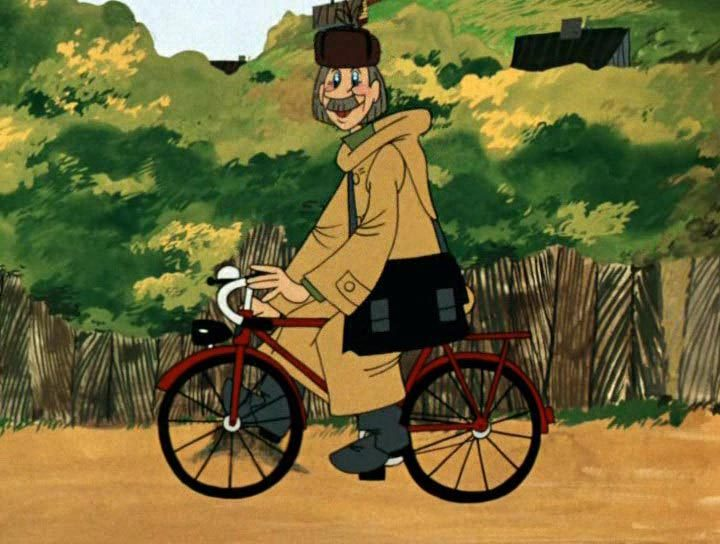
\includegraphics[scale=0.2]{Figures/pechkin.jpg}}}&{}\\
  {}&{}&{}&{}&{\rule{-2em}{0em}\text{OS}\quad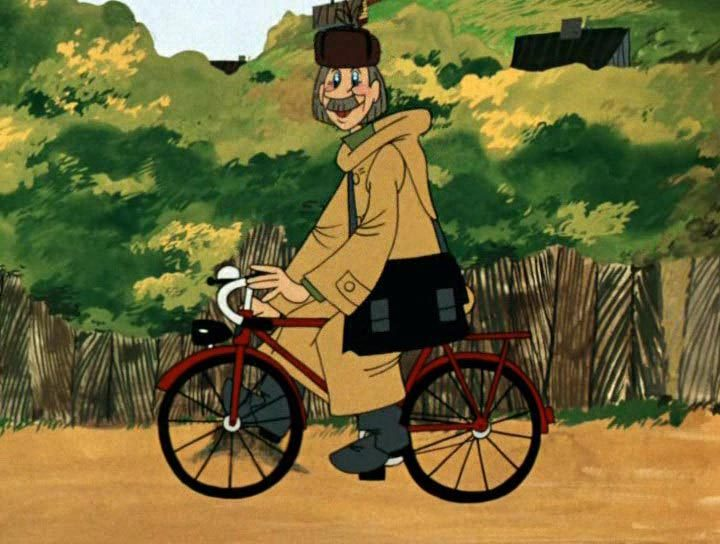
\includegraphics[scale=0.2]{Figures/pechkin.jpg}}\ar@{-->}@/^10pt/[uu]\ar@{-->}@/^10pt/[uull]\ar@{-->}@/^10pt/[uullll]&{}\\
}
\]
Здесь в роли почтальона Печкина выступает система, которая перерабатывает сообщения операционной среды в сообщения экосистемы и посылает их нужным адресатам (обозначено пунктирными стрелками).
Сплошные стрелки -- это сообщения, которые агенты посылают друг другу.
Есть разные виды подобных сред с разными гарантиями на передачу сообщений.
Но я буду рассматривать только те, которые встречаются в рамках одной физической машины.
Для меня будет важно, что системы бывают с агентами двух видов: активными и пассивными.

\paragraph{MDS с активными агентами}

Напомню, что в компьютере работу совершают ядра процессора.
На уровне операционной системы есть понятие thread-а.
Это такая сущность, которая содержит работу для ядра процессора и все необходимые данные.
И можно думать, что операционная система подсоединяет thread к ядру процессора и/или отсоединяет.
Любой thread запускается с указанием стартовой функции, которая и будет описывать работу исполняемую на ядре.

В качестве примера Message Driven System-ы с активными агентами подходит операционная система Windows.
Оказывается, что все поведение ОС из коробки построено на сообщениях.
Все сигналы в приложение от операционной системы приходят в виде сообщений.
Обмен информацией между приложениями ведется с помощью сообщений.
Когда запускается очередное приложение в операционной системе, оно запускается на новом thread-е.
При этом на этом thread-е создается почтовый ящик для получения сообщений и требуется запустить event loop.
Event loop -- это цикл, который обрабатывает сообщения если они есть в почтовом ящике, а если ничего нет, то нужно уснуть.
Соответствующую картинку можно нарисовать так:
\[
\xymatrix@R=5pt{
  {\text{App1}}&{}&{\text{App2}}&{}&{\text{App3}}\\
  {
  \begin{tabular}{c}
  mail box\\
  \begin{tabular}{|c|c|c|}
  \hline
  {}&{}&{}\\
  \hline
  \end{tabular}
  \end{tabular}
  }
  \ar@(l,l)@{-->}[dd]
  &{}&{
  \begin{tabular}{c}
  mail box\\
  \begin{tabular}{|c|c|c|}
  \hline
  {}&{}&{}\\
  \hline
  \end{tabular}
  \end{tabular}
  }
  \ar@(l,l)@{-->}[dd]
  &{}&{
  \begin{tabular}{c}
  mail box\\
  \begin{tabular}{|c|c|c|}
  \hline
  {}&{}&{}\\
  \hline
  \end{tabular}
  \end{tabular}
  }
  \ar@(l,l)@{-->}[dd]
  \\
  {
  {\text{Thread1}}
  }&{}&{
  {\text{Thread2}}
  }&{}&{
  {\text{Thread3}}
  }\\
  {
  {\text{event loop}}
  }
  \ar@(r, r)[uu]\ar@(r, l)[uurr]
  &{}&{
  {\text{event loop}}
  }
  \ar@(r, l)[uurr]
  &{}&{
  {\text{event loop}}
  }
  \ar@(r, r)[uu]
  \\
  {}&{}&{}&{}&{}\\
}
\]
Здесь каждый агент -- это отдельное приложение, которое имеет свой почтовый ящик и крутит на своем thread-е event loop.
Для полноты картины напишу как приблизительно выглядит event loop
\begin{cppcode}
int runEventLoop() {
  CMessageStatus Status;
  MSG CurrentMessage;
  while ((Status = ::GetMessage(&CurrentMessage, hwnd(), 0, 0)) != Quit) {
    if (Status == Error)
      handleError(&CurrentMessage);
    else
      ::TranslateMessage(CurrentMessage);
      ::DispatchMessage(CurrentMessage);
  }
  return exitCode(&CurrentMessage);
}
\end{cppcode}
Надо сказать, что перед запуском такого цикла обязательно должна быть команды создающие почтовый ящик, регистрирующие этот почтовый ящик в системе и прочие детали для внедрения в среду Windows.
Я весь этот код игнорирую.
Но давайте поймем  логическую структуру данного цикла.
В самом начале у нас есть две переменные для статуса и для сообщения.
Внутри \verb"while" цикла мы считываем текущее сообщение и записываем его статус в переменную \verb"Status".
Далее если статус это \verb"Quit", то мы выходим из цикла и программа завершается.
Если функция \verb"GetMessage" видит пустой ящик, то она усыпляет данный thread и цикл зависает.
Эта функциональность поддерживается автоматически из коробки.
Внутри цикла идет в начале обработчик ошибок.
А потом две стандартные функции, которые обеспечивают доставку сообщений в Windows.
Не спрашивайте меня почему их две, и почему у них такие дурацкие названия, это все следствие legacy.
Именно при вызове функции \verb"DispatchMessage" сообщение достается и отправляется в обработку.

\paragraph{MDS с пассивными агентами}
% TO DO

Примером Message Driven System-ы с пассивными агентами является экосистема Qt (читается cute).
На сегодняшний день это один из самых известных и мощных фреймворков для работы с GUI на C++.
Но как и C++, она максимально кривая и сложная для безопасного использования.
В рамках этой экосистемы выделяется один thread для event loop-а и на нем создается почтовый ящик.
Это все инкапсюлировано в объект \verb"QApplication".
Агентами в этой системе выступают \verb"QObject".
Это все возможные компоненты Qt графические и не только.
Например окно является агентом, кнопочка на нем является агентом, формы для ввода данных являются агентами и т.д.
Но все эти агенты не имеют своего thread-а для выполнения своих методов.
Вместо этого они лежат пассивно в памяти, а всю работу выполняет \verb"QApplicaion".
Думать про это надо так.
\verb"QApplication" -- это Папа Карло.
\verb"QObject"-ы -- это куча Буратин лежащих в комнате.
Что делает Папа Карло?
Во-первых, он ловит сообщения операционной системы и перерабатывает их в Qt сообщения и складывает в свой почтовый ящик.
Во-вторых, он вынимает из почтового ящика сообщения, смотри какая Буратина должна его получить.
Идет к этой буратине, и вызывает у него нужный метод.
В результате работы этого метода может быть появятся другие письма, которые будут сложены в почтовый ящик.
Давайте снабдим это описание картинкой.
\[
\xymatrix@C=15pt{
  {
  \begin{tabular}{c}
  {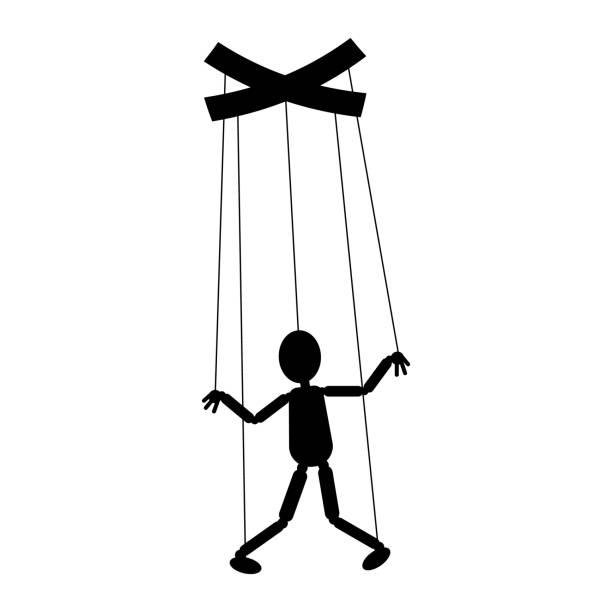
\includegraphics[scale=0.5]{Figures/marionette.jpg}}
  \\
  {\text{QObj1}}
  \end{tabular}
  }&{}&{
  \begin{tabular}{c}
  {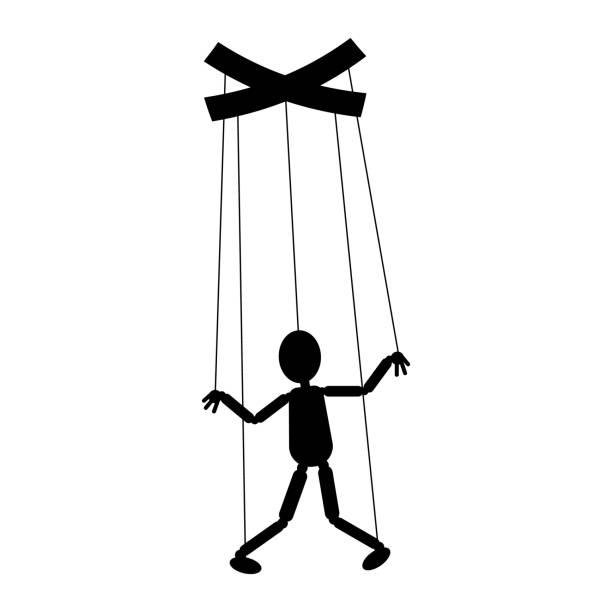
\includegraphics[scale=0.5]{Figures/marionette.jpg}}
  \\
  {\text{QObj2}}
  \end{tabular}
  }&{}&{
  \begin{tabular}{c}
  {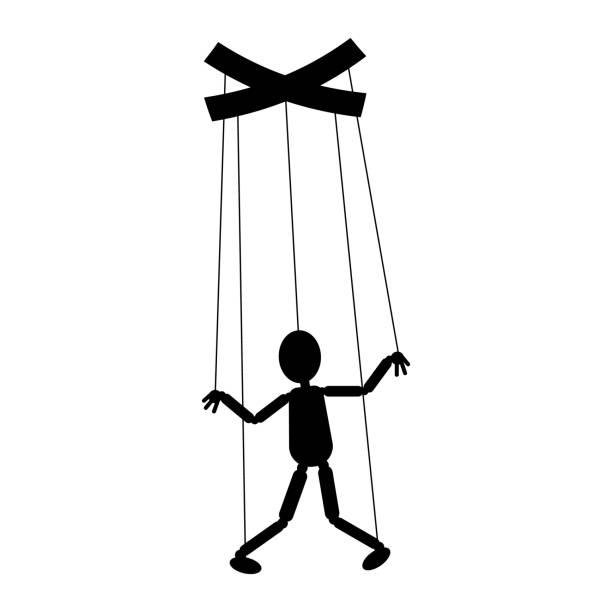
\includegraphics[scale=0.5]{Figures/marionette.jpg}}
  \\
  {\text{QObj3}}
  \end{tabular}
  }\\
  {
  \begin{tabular}{c}
  qApp\\
  Qt mail box\\
  \begin{tabular}{|c|c|c|}
  \hline
  {}&{}&{}\\
  \hline
  \end{tabular}\\
  {\textbf{Thread}}
  \end{tabular}
  }
  \ar@(r,r)[u]
  \ar@(r,d)[rru]
  \ar@(r,d)[rrrru]
  &{}&{}&{}&{
  {\textbf{OS}}
  }
  \ar@{-->}[llll]
  \\
}
\]
Так же для полноты картины давайте я приведу пример event loop в Qt экосистеме.
\begin{cppcode}
int main(int argc, char* argv[]) {
  QApplication QRunTime(argc, argv);
  Application application;
  QRunTime.exec();
  return 0;
}
\end{cppcode}
Вторая строчка создает Qt экосистему для данного thread-а.
Третья строчка создает объект приложения.
Важно, что его компоненты будут взаимодействовать с Qt экосистемой.
В этой строчке само приложение просто положили в память, корректно инициализировали и корректно подключили к Qt экосистеме.
И четвертая строчка запускает event loop.
Именно в этой функции крутится цикл, который выполняет всю работу.
В частности внутри этого цикла и будет выполняться работа при получении сообщения адресатом.

Функционирование Qt экосистемы можно представлять себе следующим образом:
\begin{center}
\begin{tabular}{rr}
{
1)\quad\scalebox{0.5}{
\boxed{
\begin{minipage}[\baselineskip]{12cm}
\[
\xymatrix@C=15pt{
  {}&{
  \begin{matrix}
  {\verb"QApplication"}\\
  {
  \begin{array}{|c|c|c|c|}
  \hline
  {\text{\color{red}\Letter}}&{\text{\Letter}}&{\ldots}&{\text{\Letter}}\\
  \hline
  \end{array}
  }
  %\ar@(l,u)[ld]
  %\ar@{<-}@(r,u)[rrdd]+(4,4)|-{\verb"postEvent"}
  \end{matrix}
  }&{}&{}\\
  {\phantom{\text{\Letter}}}
  %\ar[d]|-{\verb"event"}
  %\ar[dr]+(-4,15)|-{\verb"event"}
  %\ar[drrr]+(-4,15)|-{\verb"event"}&{}&{}&{}
  \\
  {
  \begin{matrix}
  {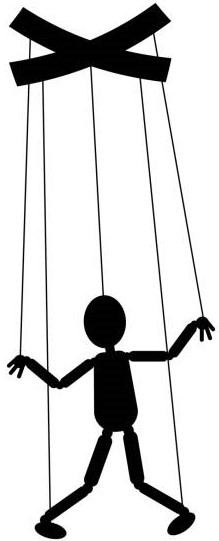
\includegraphics[scale=0.5]{Figures/marionette1.jpg}}\\
  {\verb"QObject1"}
  \end{matrix}
  }&{
  \begin{matrix}
  {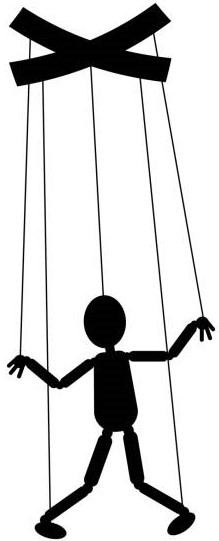
\includegraphics[scale=0.5]{Figures/marionette1.jpg}}\\
  {\verb"QObject2"}
  \end{matrix}
  }&{
  \begin{matrix}
  {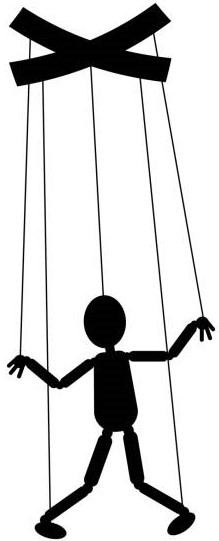
\includegraphics[scale=0.5]{Figures/marionette1.jpg}}\\
  {\verb"QObject3"}
  \end{matrix}
  }&{
  \begin{matrix}
  {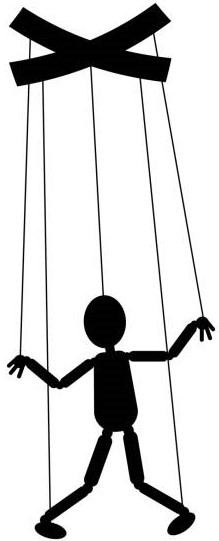
\includegraphics[scale=0.5]{Figures/marionette1.jpg}}\\
  {\verb"QObject4"}
  \end{matrix}
  }\\
}
\]
\end{minipage}
}}
}&{
5)\quad\scalebox{0.5}{
\boxed{
\begin{minipage}[\baselineskip]{12cm}
\[
\xymatrix@C=15pt{
  {}&{
  \begin{matrix}
  {\verb"QApplication"}\\
  {
  \begin{array}{|c|c|c|c|}
  \hline
  {\phantom{\text{\Letter}}}&{\text{\Letter}}&{\ldots}&{\text{\Letter}}\\
  \hline
  \end{array}
  }
  %\ar@(l,u)[ld]
  %\ar@{<-}@(r,u)[rrdd]+(4,4)|-{\verb"postEvent"}
  \end{matrix}
  }&{}&{}\\
  {{\text{\Letter}}}
  %\ar@[red][d]|-{\verb"event"}
  %\ar@[red][dr]+(-4,15)|-{\verb"event"}
  \ar@[red][drrr]+(-4,15)|-{\verb"event"}&{}&{}&{}
  \\
  {
  \begin{matrix}
  {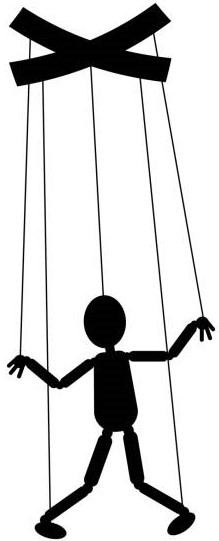
\includegraphics[scale=0.5]{Figures/marionette1.jpg}}\\
  {\verb"QObject1"}
  \end{matrix}
  }&{
  \begin{matrix}
  {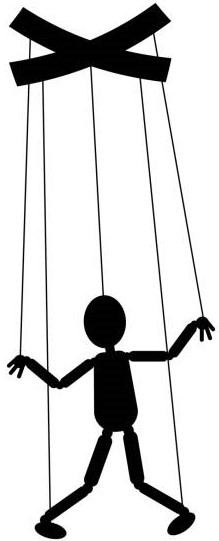
\includegraphics[scale=0.5]{Figures/marionette1.jpg}}\\
  {\verb"QObject2"}
  \end{matrix}
  }&{
  \begin{matrix}
  {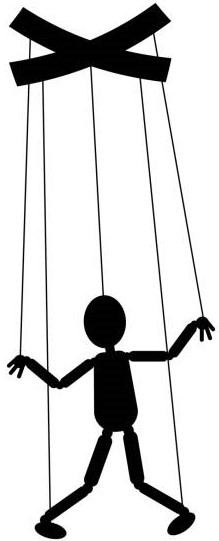
\includegraphics[scale=0.5]{Figures/marionette1.jpg}}\\
  {\verb"QObject3"}
  \end{matrix}
  }&{
  \begin{matrix}
  {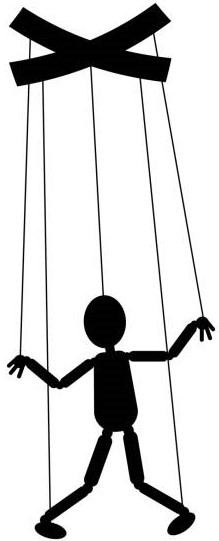
\includegraphics[scale=0.5]{Figures/marionette1.jpg}}\\
  {\verb"QObject4"}
  \end{matrix}
  }\\
}
\]
\end{minipage}
}}
}\\
{
2)\quad\scalebox{0.5}{
\boxed{
\begin{minipage}[\baselineskip]{12cm}
\[
\xymatrix@C=15pt{
  {}&{
  \begin{matrix}
  {\verb"QApplication"}\\
  {
  \begin{array}{|c|c|c|c|}
  \hline
  {\phantom{\text{\Letter}}}&{\text{\Letter}}&{\ldots}&{\text{\Letter}}\\
  \hline
  \end{array}
  }
  \ar@(l,u)[ld]
  %\ar@{<-}@(r,u)[rrdd]+(4,4)|-{\verb"postEvent"}
  \end{matrix}
  }&{}&{}\\
  {{\text{\color{red}\Letter}}}
  %\ar[d]|-{\verb"event"}
  %\ar[dr]+(-4,15)|-{\verb"event"}
  %\ar[drrr]+(-4,15)|-{\verb"event"}&{}&{}&{}
  \\
  {
  \begin{matrix}
  {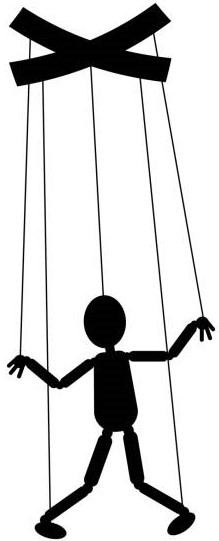
\includegraphics[scale=0.5]{Figures/marionette1.jpg}}\\
  {\verb"QObject1"}
  \end{matrix}
  }&{
  \begin{matrix}
  {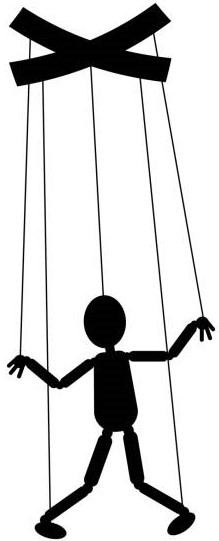
\includegraphics[scale=0.5]{Figures/marionette1.jpg}}\\
  {\verb"QObject2"}
  \end{matrix}
  }&{
  \begin{matrix}
  {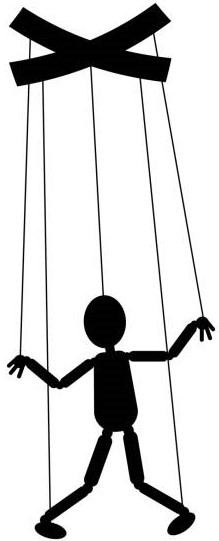
\includegraphics[scale=0.5]{Figures/marionette1.jpg}}\\
  {\verb"QObject3"}
  \end{matrix}
  }&{
  \begin{matrix}
  {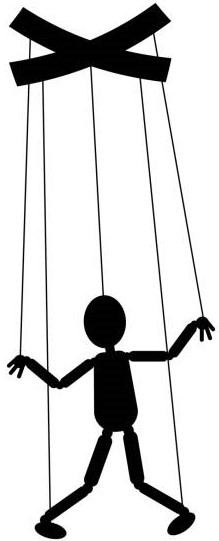
\includegraphics[scale=0.5]{Figures/marionette1.jpg}}\\
  {\verb"QObject4"}
  \end{matrix}
  }\\
}
\]
\end{minipage}
}}
}&{
6)\quad\scalebox{0.5}{
\boxed{
\begin{minipage}[\baselineskip]{12cm}
\[
\xymatrix@C=15pt{
  {}&{
  \begin{matrix}
  {\verb"QApplication"}\\
  {
  \begin{array}{|c|c|c|c|}
  \hline
  {\phantom{\text{\Letter}}}&{\text{\Letter}}&{\ldots}&{\text{\Letter}}\\
  \hline
  \end{array}
  }
  %\ar@(l,u)[ld]
  \ar@{<-}@(r,u)@[red][rrdd]+(4,4)|-{\verb"postEvent"}
  \end{matrix}
  }&{}&{}\\
  {{\text{\Letter}}}
  %\ar@[red][d]|-{\verb"event"}
  %\ar@[red][dr]+(-4,15)|-{\verb"event"}
  \ar[drrr]+(-4,15)|-{\verb"event"}&{}&{}&{}
  \\
  {
  \begin{matrix}
  {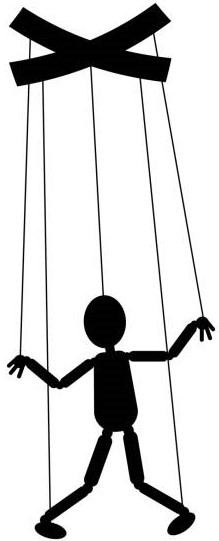
\includegraphics[scale=0.5]{Figures/marionette1.jpg}}\\
  {\verb"QObject1"}
  \end{matrix}
  }&{
  \begin{matrix}
  {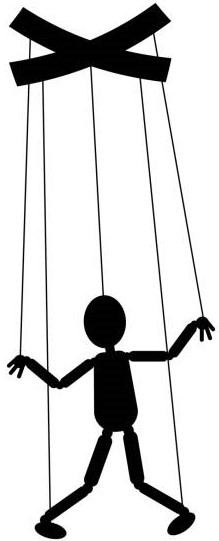
\includegraphics[scale=0.5]{Figures/marionette1.jpg}}\\
  {\verb"QObject2"}
  \end{matrix}
  }&{
  \begin{matrix}
  {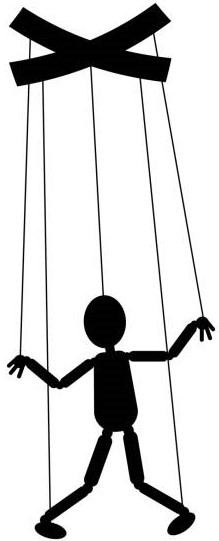
\includegraphics[scale=0.5]{Figures/marionette1.jpg}}\\
  {\verb"QObject3"}
  \end{matrix}
  }&{
  \begin{matrix}
  {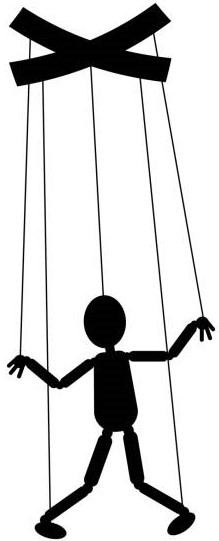
\includegraphics[scale=0.5]{Figures/marionette1.jpg}}\\
  {\verb"QObject4"}
  \end{matrix}
  }\\
}
\]
\end{minipage}
}}
}\\
{
3)\quad\scalebox{0.5}{
\boxed{
\begin{minipage}[\baselineskip]{12cm}
\[
\xymatrix@C=15pt{
  {}&{
  \begin{matrix}
  {\verb"QApplication"}\\
  {
  \begin{array}{|c|c|c|c|}
  \hline
  {\phantom{\text{\Letter}}}&{\text{\Letter}}&{\ldots}&{\text{\Letter}}\\
  \hline
  \end{array}
  }
  %\ar@(l,u)[ld]
  %\ar@{<-}@(r,u)[rrdd]+(4,4)|-{\verb"postEvent"}
  \end{matrix}
  }&{}&{}\\
  {{\text{\Letter}}}
  \ar@[red][d]|-{\verb"event"}
  %\ar[dr]+(-4,15)|-{\verb"event"}
  %\ar[drrr]+(-4,15)|-{\verb"event"}&{}&{}&{}
  \\
  {
  \begin{matrix}
  {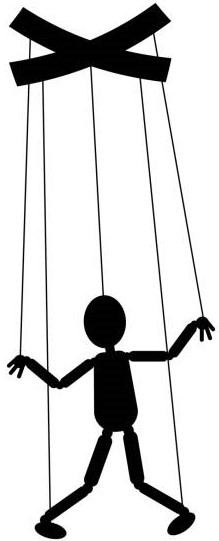
\includegraphics[scale=0.5]{Figures/marionette1.jpg}}\\
  {\verb"QObject1"}
  \end{matrix}
  }&{
  \begin{matrix}
  {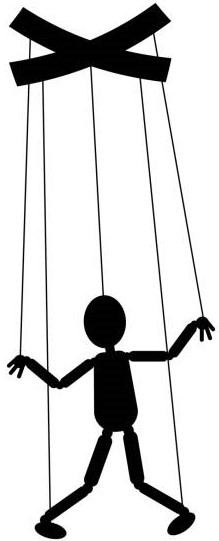
\includegraphics[scale=0.5]{Figures/marionette1.jpg}}\\
  {\verb"QObject2"}
  \end{matrix}
  }&{
  \begin{matrix}
  {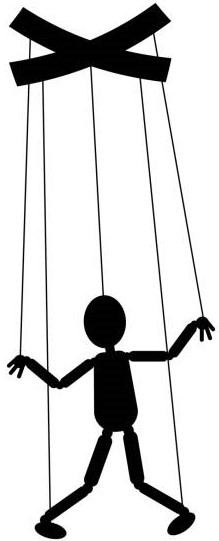
\includegraphics[scale=0.5]{Figures/marionette1.jpg}}\\
  {\verb"QObject3"}
  \end{matrix}
  }&{
  \begin{matrix}
  {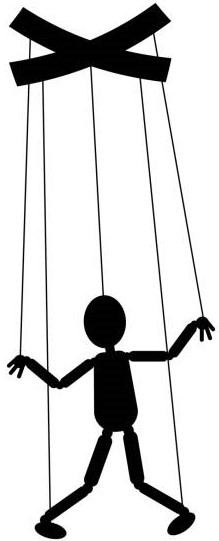
\includegraphics[scale=0.5]{Figures/marionette1.jpg}}\\
  {\verb"QObject4"}
  \end{matrix}
  }\\
}
\]
\end{minipage}
}}
}&{
7)\quad\scalebox{0.5}{
\boxed{
\begin{minipage}[\baselineskip]{12cm}
\[
\xymatrix@C=15pt{
  {}&{
  \begin{matrix}
  {\verb"QApplication"}\\
  {
  \begin{array}{|c|c|c|c|}
  \hline
  {{\text{\Letter}}}&{\text{\Letter}}&{\ldots}&{\text{\color{red}\Letter}}\\
  \hline
  \end{array}
  }
  %\ar@(l,u)[ld]
  \ar@{<-}@(r,u)[rrdd]+(4,4)|-{\verb"postEvent"}
  \end{matrix}
  }&{}&{}\\
  {{\text{\Letter}}}
  %\ar@[red][d]|-{\verb"event"}
  %\ar@[red][dr]+(-4,15)|-{\verb"event"}
  \ar[drrr]+(-4,15)|-{\verb"event"}&{}&{}&{}
  \\
  {
  \begin{matrix}
  {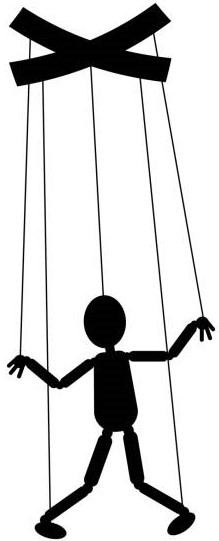
\includegraphics[scale=0.5]{Figures/marionette1.jpg}}\\
  {\verb"QObject1"}
  \end{matrix}
  }&{
  \begin{matrix}
  {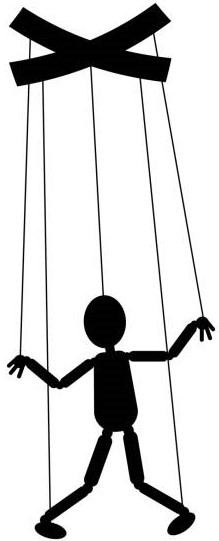
\includegraphics[scale=0.5]{Figures/marionette1.jpg}}\\
  {\verb"QObject2"}
  \end{matrix}
  }&{
  \begin{matrix}
  {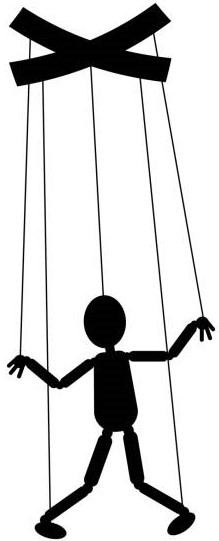
\includegraphics[scale=0.5]{Figures/marionette1.jpg}}\\
  {\verb"QObject3"}
  \end{matrix}
  }&{
  \begin{matrix}
  {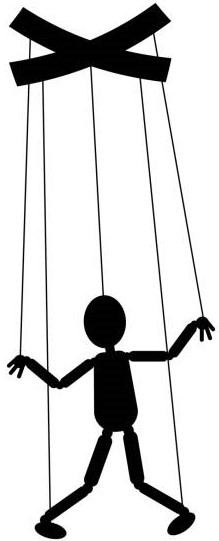
\includegraphics[scale=0.5]{Figures/marionette1.jpg}}\\
  {\verb"QObject4"}
  \end{matrix}
  }\\
}
\]
\end{minipage}
}}
}\\
{
4)\quad\scalebox{0.5}{
\boxed{
\begin{minipage}[\baselineskip]{12cm}
\[
\xymatrix@C=15pt{
  {}&{
  \begin{matrix}
  {\verb"QApplication"}\\
  {
  \begin{array}{|c|c|c|c|}
  \hline
  {\phantom{\text{\Letter}}}&{\text{\Letter}}&{\ldots}&{\text{\Letter}}\\
  \hline
  \end{array}
  }
  %\ar@(l,u)[ld]
  %\ar@{<-}@(r,u)[rrdd]+(4,4)|-{\verb"postEvent"}
  \end{matrix}
  }&{}&{}\\
  {{\text{\Letter}}}
  %\ar@[red][d]|-{\verb"event"}
  \ar@[red][dr]+(-4,15)|-{\verb"event"}
  %\ar[drrr]+(-4,15)|-{\verb"event"}&{}&{}&{}
  \\
  {
  \begin{matrix}
  {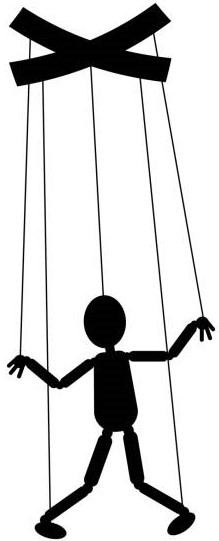
\includegraphics[scale=0.5]{Figures/marionette1.jpg}}\\
  {\verb"QObject1"}
  \end{matrix}
  }&{
  \begin{matrix}
  {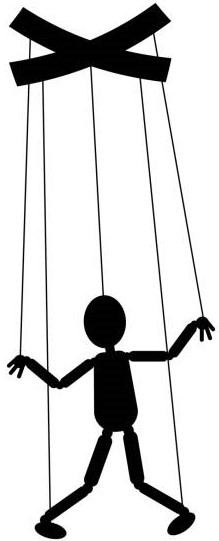
\includegraphics[scale=0.5]{Figures/marionette1.jpg}}\\
  {\verb"QObject2"}
  \end{matrix}
  }&{
  \begin{matrix}
  {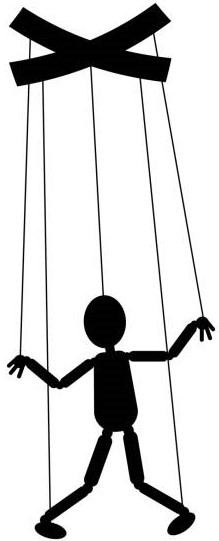
\includegraphics[scale=0.5]{Figures/marionette1.jpg}}\\
  {\verb"QObject3"}
  \end{matrix}
  }&{
  \begin{matrix}
  {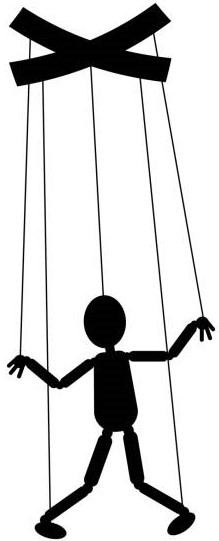
\includegraphics[scale=0.5]{Figures/marionette1.jpg}}\\
  {\verb"QObject4"}
  \end{matrix}
  }\\
}
\]
\end{minipage}
}}
}&{
}\\
\end{tabular}
\end{center}
Прокомментируем поведение системы выше:
\begin{enumerate}
\item \verb"QApplication" проверяет пуст ли почтовый ящик или нет.
Если почтовый ящик пуст, то система засыпает пока не появятся сообщения от операционной системы.
Эти сообщения будут трансформированы в Qt сообщения и сложены в почтовый ящик.

\item Если почтовый ящик не пуст, то вынимаем первое сообщение из ящика.
Теперь можно совершать доставку сообщения адресатам

\item В Qt экосистеме обработчик сообщения у адресата -- функция \verb"event".
Вызываем эту функцию для \verb"QObject1" и передаем в нее текущее сообщение.

\item Теперь вызываем \verb"event" у \verb"QObject2" и передаем в нее текущее сообщение.

\item На этом шаге вызываем \verb"event" у \verb"QObject4" и передаем в нее текущее сообщение.

\item В результате обработки сообщения \verb"QObject4" сформировал сообщение и отправляет его в почтовый ящик \verb"QApplication".

\item Сообщение от \verb"QObject4" положили в конец очереди в почтовый ящик.
На этом одна итерация event loop-а завершается и весь процесс повторяется с самого начала.
\end{enumerate}


\subsubsection{Идея имплементации}

Я уже приводил пример event loop-а для двух Message Driven System.
Давайте я в общих чертах скажу, как строится произвольная такая система.
Прежде всего у нас должен почтовый ящик и event loop, которые выглядят как-то так.
\begin{cppcode}
MailBox gBox;

int main() {
  Event e;
  while(getEvent(&e)) {
    dispatchEvent(e);
  }
  return 0;
}
\end{cppcode}
Тут важно понимать, что почтовый ящик является глобальным ресурсом для данного thread-а.
Как мы видим весь event loop устроен очень просто, мы вынимаем сообщение из почтового ящика в функции \verb"getEvent".
А потом запускаем доставку сообщений в методе \verb"dispatchEvent".
При такой имплементации цикл заканчивается, если \verb"getEvent" вернет \verb"false".
В этой имплементации отсутствует код, перерабатывающий сообщения операционной системы в сообщения экосистемы.

Функция доставки сообщений работает приблизительно так
\begin{cppcode}
void dispatchEvent(const Event& e) {
  for (auto obj : addresseesOf(e)) {
    obj->handleEvent(e);
  }
}
\end{cppcode}
То есть для каждого сообщения составляется список его адресатов, а потом мы просто зовем служебную функцию \verb"handleEvent" у всех адресатов блокирующим образом.

Теперь, что из себя представляет сообщение?
Обычно это данные и некоторая метаинформация, которая помогает понять, что это за данные.
Ведь передавать мы должны уметь все что угодно.
Кратко можно думать про это так
\begin{cppcode}
enum class EventType {
  Mouse,
  Keyboard,
  /* ... */};

class Event {
public:
  /*Constructor*/
  EventType type() const;
  const void* data() const;
  
private:
  EventType type_;
  std::any data_;
};
\end{cppcode}
Здесь \verb"EventType" -- это заранее известный набор констант для всех возможных типов сообщений.
Многие системы имеют выделенный диапазон типов для создания пользовательских сообщений.
Само сообщение содержит информацию о типе и данные.
Я использую \verb"std::any" как стирающий тип, который умеет хранить что угодно.

Теперь перейдем к обработке сообщений.
Для хранения списка адресатов, который используется в функции \verb"dispatchEvent" можно использовать интерфейсы или стирающие ссылки.
\begin{cppcode}
std::vector<EventHandler> addresseesOf(const Event& e)
\end{cppcode}
здесь \verb"EventHandler" -- это стирающий указатель на объект, которому доставляется сообщение.
Для попадания в этот список в системе должны быть свои механизмы, которые я тут не собираюсь обсуждать.
Теперь обработка сообщений выглядит как-то так
\begin{cppcode}
class Obj1 {
public:
  void handleEvent(const Event& e) override {
    switch(e.type()) {
      case EventType::Mouse:
        MouseEvent& Data = cast<MouseEvent&>(e.data());
        // handle mouse event
      break;
      case EventType::Keyboard:
        KeyboardEvent& Data = cast<KeyboardEvent&>(e.data());
        // handle keyboard event
      break;
      ...
    }
  }
};
\end{cppcode}
Каждый объект должен прочитать тип сообщения, а потом в зависимости от этой информации вынуть нужные данные и отреагировать на них.
Возможно, что \verb"handleEvent" игнорирует какие-то сообщения, а может быть даже и все.
Функция \verb"cast" выше -- это псевдокод, который призван показать, что мы вынимаем из сообщения данные, которые там зашифрованы в зависимости от информации о типе сообщения.

\subsubsection{Неблокирующие операции}
% TO DO

Теперь, если мы орудуем в рамках Message Driven System, у нас есть два способа отправить данные из одной функции в другую.
\begin{enumerate}
\item Прямой блокирующий вызов.
Этот случай -- это просто обычный вызов функции внутри другой функции.
Например, если работает обработчик сообщений \verb"Obj1", то он может дернуть (если знает адрес) какой-нибудь метод из \verb"Obj2".
В этом случае реакция на данные происходит немедленно.

\item Посылка сообщения.
В этом случае если обработчик сообщений \verb"Obj1" произвел какие-то данные для \verb"Obj2", то он не вызывает метод \verb"Obj2".
Вместо этого он создает сообщение, куда складывает эту информацию, пишет в качестве адресата \verb"Obj2" на конверте и складывает письмо в почтовый ящик.
В этом случае реакция на сообщение произойдет не сразу же во время отправки сообщения, а позже, когда экосистема дойдет до обработки сообщения и передаст его адресату.
Такое поведение называется неблокирующим вызовом.
Это поведение важно держать в голове, потому что важно поместить в сообщение все данные, чтобы они были живы, когда сообщение дойдет до адресата.
Нельзя вкладывать ссылки и указатели на локальные данные, просто потому что они все умрут к моменту передачи сообщения по назначению.
\end{enumerate}
Второй подход нужен для того, чтобы не блокировать на долго одной задачей ядро процессора.
Чтобы на одном ядре успевали покрутиться разные обработчики сообщений.
Это делается для того, чтобы GUI был отзывчивым и окна не подвисали.
В рамках такой экосистемы полезно иметь неблокирующий observer pattern, в котором observable не сразу дергает методы \verb"onSubscribe" и \verb"onNotify", а посылает сообщения через Message Driven System.

\subsection{Неблокирующий Observer Pattern}
\label{section::ObserverNonBlocking}

\subsubsection{Общая схема}

Для неблокирующего observer pattern нам прежде всего нужна некоторая Message Driven System, которая будет использоваться для пересылки сообщений.
Грубо общую модель можно описать следующей диаграммой.

\[
\xymatrix{
  {\vphantom{\text{Message System}}}
    {\save
  [].[rr]*+[F--]\frm{}
  \restore
  }  
  &{\text{Message System}}\ar[rd]\ar[rdd]&{}\\
  {\text{Observable}}\ar[ru]<-0.5em>\ar[ru]&{}&{\text{Observer0}}\\
  {}&{}&{\text{Observer1}}\\
}
\]
В рамках такой системы \verb"Observable" не дергает методы \verb"Observer" напрямую.
Вместо этого он посылает данные в виде сообщения каждому \verb"Observer"-у.
Давайте отметим несколько интересных изменений, которые возникают из-за такой системы.
\begin{itemize}
\item Прежде всего, нужен механизм адресации для того, чтобы можно было отправлять сообщения конкретным объектам.
Обычно в любой Message Driven System такая возможность имеется из коробки и тут не надо ничего изобретать.

\item В зависимости от возможностей Message Driven System-ы бывает нужно уметь проверять жив ли объект, которому отправляется сообщение.
Причем жив ли он не в момент отправки, а в момент доставки сообщения.
Например в системе Qt таких гарантий нет.

\item Так как сообщения посылаются разными сообщениями каждый своему адресату, то не возможно пересылать данные по ссылке.
Приходится в каждое сообщение от \verb"Observable" вкладывать копию данных, которые надо пересылать.

\item Когда же сообщение доставляется \verb"Observer", то мы гарантируем, что получатель ровно один и больше сообщение не понадобится.
В этом случае данные можно безболезненно вынуть (мувнуть) из сообщения.

\item Обратите внимание, что общение между \verb"Observer" и \verb"Observable" теперь происходит не мгновенно блокирующим образом, а с задержками.
Они не реагируют друг на друга мгновенно.
В этом случае можно думать, что общение портов происходит как бы через сеть.
А все сетевое взаимодействие принято описывать с помощью State Machine.
\end{itemize}
Важно помнить, что конкретная имплементация зависит от выбора Message Driven System, от ее возможностей и предоставляемых гарантий.

\subsubsection{Передача данных поверх Qt}

\paragraph{Дефекты Qt}

Начать я хочу с важного замечания по поводу системы Qt.
Когда \verb"QApplication" доставляет сообщения адресатам
\[
\xymatrix{
  {\verb"QApplication"}\ar[rr]^{\verb"event"}&{}&{\verb"QObject"}\\
}
\]
он дергает блокирующим образом метод \verb"event" по адресу объекта получателя.
Однако, нет никаких гарантий, что объект, у которого мы дергаем \verb"event" еще жив.
Вокруг этой проблемы есть огромное количество костылей в Qt, включая отложенное удаление объекта.
Получается, что в Qt экосистеме нельзя просто так слать сообщение \verb"QObject" напрямую.
Нужно перед дерганьем метода \verb"event" проверить жив ли объект.
И в Qt есть специальный следящий указатель (который по сути является другой имплементацией следящего указателя из раздела~\ref{section::TrackingPtr}) и называется он \verb"QPointer".
Так же важно, что объект \verb"QApplication" всегда жив (на основном thread-е конечно).
Тогда правильная схема -- отправить сначала сообщение \verb"QApplication" на своем thread-е.
Если получатель живет на этом же thread-е, то \verb"QApplication" в начале проверяет жив ли адресат и после этого дергает у него \verb"event".
Если же нужно послать сообщение другому thread-у, то тут надо огранизовывать взаимодействие между \verb"QApplication" на разных thread-ах.
Благо Qt дает некую поддержку из коробки для этого.
Но я не хочу это обсуждать.

\paragraph{QPort}

Обратите внимание, что сейчас обсуждается задача безопасной пересылки сообщения в экосистеме Qt.
Этой проблемы может не быть в других экосистемах, но так и хорошо, я смогу продемонстрировать как подобные вещи решаются.
Так как это задача более низкоуровневая, чем observer pattern, то здесь речь будет идти о более простом примитиве, который я хочу назвать \verb"QPort".
Его задача будет состоять лишь в том, чтобы уметь передавать безопасно данные из от одного порта к другому не блокирующим образом.
Ничего другого эти порты уметь не будут.
И уже поверх этих портов мы построим observer pattern.
Давайте схематично изобразим, что из себя представляет сообщение и как оно передается.
\[
\xymatrix@R=15pt{
  {}&{}&{\verb"QApplication"}
  \ar@{=>}@(r,u)[rdd]^{2}
  &{}
  \\
  {}&{{\verb"Message"}}
  \ar@{=>}@(u,l)[ur]^{1}
  {\save
  [].[ddd]*+[F-]\frm{}
  \restore
  }
  &{}&{}\\
  {{\verb"QPort"}}&
  {{\verb"QPtr from"}}
  \ar[l]
  {\save
  [].[dd]*[F-]\frm{}
  \restore
  }
  &{}&{\verb"QPort"}\\
  {}&{{\verb"QPtr to"}}
  \ar[rru]
  &{}&{}\\
  {}&{{\verb"any data"}}&{}&{}\\
}
\]
\begin{enumerate}
\item Сообщение \verb"Message" содержит три поля
\begin{enumerate}
\item Адрес порта отправителя в виде \verb"QPointer".
Адрес отправителя нам понадобится для двусторонней коммуникации в observer pattern.

\item Адрес порта получателя в виде \verb"QPointer".

\item И сами данные в виде стирающего типа \verb"std::any".
Это означает, что пользователь портов должен знать, что он отправляет и написать весь функционал поддерживающий типизацию поверх этой системы.
\end{enumerate}
Тут надо сказать зачем данные отправляются в виде \verb"std::any".
Почему мы не используем шаблонный порт \verb"QPort<T>", что гарантировало бы доставку сообщений определенного типа.
Тут к сожалению выстреливает еще одна особенность именно экосистемы Qt.
Дело в том, что для правильной работы Qt выполняет генерацию кода для каждого \verb"QObject".
Для этого есть специальный метакомпилятор \verb"moc".
И метакомпилятор всегда применяется к \verb"cpp" файлам и никогда не применяется к хедерам.
Но шаблон нельзя разделить на хедер и сурс.
Потому приходится обходиться без шаблонов с помощью стирающих типов.

\item Порт отправитель не шлет сообщение напрямую порту получателю, вместо этого сообщение отправляется \verb"QApplication" по стрелке (1).
Это действие всегда безопасно, потому что Qt экосистема гарантируется, что \verb"QApplication" будет жить, если жив на данном thread-е дольше всех остальных объектов.
Он создается первым, и удаляется последним.
Межthread-овая коммуникация требует некоторой отдельной работы.

\item Теперь нам надо будет внести модификацию в поведение \verb"QApplication", чтобы он умел переотправлять наши сообщения порту получателю.
Идея в том, что в начале \verb"QApplication" проверяет \verb"QPointer" получателя.
Так как получатель живет на этом же thread-е, то у нас нет гонки между деструктором получателя и обработкой сообщения.
Либо одно либо другое происходит раньше.
Потому \verb"QApplication" может спокойно проверить \verb"QPointer" и если он не \verb"nullptr", то можно дернуть по его адресу метод \verb"event".
\end{enumerate}

\paragraph{Сообщения}
% TO DO

Все сообщения в Qt экосистеме должны быть унаследованы публично от \verb"QEvent".
Как было изображено на диаграмме мы должны иметь
\begin{cppcode}
class Message : public QEvent {
public:
  using CPointer = QPointer<QEvent>;
  ...
private:
  CPointer from_;
  CPointer to_;
  std::any data_;
};
\end{cppcode}
Кроме того, у каждого сообщения есть идентификатор \verb"QEvent::Type", который представляет из себя целое число.
Это просто тег, который говорит получателю, что это за сообщения, чтобы потом суметь вынуть данные.
Экосистема Qt позволяет зарегистрировать автоматически первый свободный идентификатор.
Для этого выделим статический метод, который зарегистрирует тип при первом вызове и будет возвращать его значение всюду далее.
\begin{cppcode}
class Message : public QEvent {
public:
  static QEvent::Type type() {
    static int message_type = registerEventType();
    return QEvent::Type{message_type};
  }
  ...
private:
  ...
};
\end{cppcode}
Напишем полностью интерфейс класса
\begin{cppcode}
class Message : public QEvent {
public:
  using CPointer = QPointer<QObject>;
  static QEvent::Type type();
  
  Message(CPointer from, CPointer to, const std::any& data);
  Message(CPointer from, CPointer to, std::any&& data);
  
  std::any&& extract();
  
  bool isReceiverAlive() const;
  
  CPointer receiver() const;
  CPointer to() const;
  CPointer from() const;
private:
  CPointer from_;
  CPointer to_;
  std::any data_;
};
\end{cppcode}
В начале покажем, как нужно написать конструкторы
\begin{cppcode}
Message(CPointer from, CPointer to, const std::any& data)
  : QEvent(type()), from_(std::move(from)), to_(std::move(to)),
    data_(data) {}
Message(CPointer from, CPointer to, std::any&& data)
  : QEvent(type()), from_(std::move(from)), to_(std::move(to)),
    data_(std::move(data)) {}
\end{cppcode}
Тут все просто, мы вызываем базовый конструктор, в который передаем тип сообщения вызывая статическую функцию \verb"type".
Нам нужны два конструктора, чтобы была возможность положить новые данные в сообщения или мувнуть туда уже существующие.
Теперь имплементация оставшихся методов
\begin{cppcode}
class Message : public QEvent {
public:
  ...
  std::any&& extract() {
    return std::move(data_);
  }
  bool isReceiverAlive() const {
    return to_;
  }
  CPointer receiver() const {
    return to_;
  }
  CPointer to() const {
    return to_;
  }
  CPointer from() const {
    return from_;
  }
private:
  ...
};
\end{cppcode}
Тут все просто кроме быть может метода \verb"extract".
Дело в том, что когда сообщение приходит в порт назначения, то оно больше использоваться не будет.
А значит, нам надо вынуть данные из сообщения.
Для этого нужно мувнуть данные наружу.
Тут есть две опции:
\begin{enumerate}
\item Вернуть \verb"std::any&&".

\item Вернуть \verb"std::any".
\end{enumerate}
Но в любом случае нужно будет вокруг \verb"data_" добавить \verb"std::move(data_)".
Это чуть ли ни единственный пример, когда нужно писать \verb"std::move" в \verb"return".
Без этого каста, будет сниматься копия с данных во второй имплементации.
А первая имплементация выдаст ошибку компиляции.

\paragraph{Имплементация QPort}

Начнем с интерфейса
\begin{cppcode}
class QPort : public QObject {
  Q_OBJECT
public:
  using Message = detail::Message;
  using CPointer = Message::CPointer;

  void send(CPointer from, CPointer to, std::any data) const;
  bool event(QEvent* event) override;

protected:
  virtual void action(CPointer from, std::any&& data) = 0;

private:
  static constexpr bool k_is_processed = true;
};
\end{cppcode}
Давайте прокомментируем, что тут происходит.
Прежде всего, чтобы быть участником Qt экосистемы и уметь получать сообщения от системы нужно публично унаследоваться от \verb"QObject".
Однако, этого мало.
Из-за кодогенерации, нужно для каждого такого участника экосистемы сгенерировать некоторые служебные данные, без которых взаимодействие с системой не возможно.
Для этого служит макрос \verb"Q_OBJECT", который добавляется сразу же в приватную часть класса.

Обратите внимание, что я страшный сторонник type erasure и ненавистник наследования с виртуальными методами внезапно начинаю использовать виртуальные методы.
Связано это с тем, что в основе дизайна Qt лежит возможность наследоваться от базового класса, модифицируя его поведение переопределением виртуальных методов.
Если фреймворк использует такой подход, то использовать стирающие типы будет очень сложно, код будет менее читаемым и громоздским и скорее всего еще и будет менее эффективным.
Потому раз этот фреймворк использует такой подход, то нужно придерживаться его при взаимодействии с этим фреймворком.
Но вот снаружи я могу использовать любые парадигмы, которые захочу.

Метода \verb"action" является чисто виртуальным.
Это действие, которое будет выполняться при получении сообщения.
Обратите внимание, что данные получаются по rvalue ссылке, что означает, что мы будем вынимать данные из сообщения и передавать в этот метод через мув.
Этот метод должен быть перегружен у наследника, какими будут \verb"Observable" и \verb"Observer".

Теперь как имплементируется метод отправки сообщения
\begin{cppcode}
void QPort::send(CPointer from, CPointer to, std::any data) const {
  QCoreApplication::postEvent(
      QCoreApplication::instance(), // to whom
      new Message(std::move(from), std::move(to), std::move(data)));
}
\end{cppcode}
Тут надо обратить внимание на то, что внутри вызывается всего лишь одна функция Qt экосистемы \verb"postEvent", которая просто помещает сообщение в почтовый ящик.
Эта функция принимает два аргумента:
\begin{enumerate}
\item Адрес получателя, как адрес объекта.
Здесь мы пишем адрес текущего \verb"QApplication".
Этот объект обеспечивает существование и функционирование Qt экосистемы на данном thread-е и потому ему письмо всегда можно доставить безопасно.

\item Сообщение передаваемый по указателю.
Сообщение обязано быть унаследовано от \verb"QEvent".
Пусть вас не смущает голое \verb"new" в коде.
Данная функция захватывает владение сообщением и гарантирует его корректный менеджмент.
При работе Qt всегда приходится думать кто кем владеет, чтобы случайно не было утечек данных.
\end{enumerate}

И в теперь надо обсудить обработку входящих сообщений портом в функции \verb"event":
\begin{cppcode}
static constexpr bool k_is_processed = true;

bool QPort::event(QEvent* event) {
  if (event->type() == Message::type()) {
    Message* msg = static_cast<Message*>(event);
    action(msg->from(), msg->extract());
    return k_is_processed;
  }
  return QObject::event(event);
}
\end{cppcode}
Все что тут происходит мы смотрим на получаемое сообщение и если оно нужного нам типа, то мы вынимаем из него данные и уже скармливаем эти данные функции \verb"action", которую мы обсудили выше.

\paragraph{Поддержка сообщений со стороны Qt}

На самом деле, чтобы эта схема работала нужно еще внести дополнительные изменения в \verb"QApplication", чтобы он знал, как реагировать на наши сообщения.
Это тоже делается наследованием от \verb"QApplication".
Все что мы сделаем -- добавим правило обработки сообщений в самое начало.
Это делается с помощью функции \verb"eventFilter".
В коде это выглядит так
\begin{cppcode}
class QRunTime : public QApplication {
public:
  QRunTime(int& argc, char** argv);
private:
  bool eventFilter(QObject* obj, QEvent* event) override;
};
\end{cppcode}
Я специально меняю название на \verb"QRunTime", потому что по смыслу это именно run-time системы на данном thread-е, а не одно приложение.
Конструктор должен установить на себя же фильтр, который представляет из себя действие, которое будет производиться над сообщением до всех остальных действий.
\begin{cppcode}
QRunTime(int& argc, char** argv) : QApplication(argc, argv) {
  installEventFilter(this);
}
\end{cppcode}
Функция \verb"installEventFilter" прикрепила к \verb"this" его же самого как фильтрующий объект.
А метод, который будет вызываться для фильтрации надо имплементировать в \verb"eventFilter".
\begin{cppcode}
bool eventFilter(QObject* obj, QEvent* event) override {
  using Message = QApp::Library::QPort::Message;
  if (event->type() == Message::type()) {
    Message* msg = static_cast<Message*>(event);
    if (msg->isReceiverAlive())
      msg->receiver()->event(event);
    return true; // stop processing the event
  }
  return QApplication::eventFilter(obj, event);
}
\end{cppcode}
Все что мы делаем -- проверяем тип сообщения.
Если это наше особое сообщение для порта, то мы проверяем жив ли получатель, что делается через \verb"QPointer" внутри метода \verb"isReceiverAlive".
После чего напрямую дергаем обработчик сообщения у получателя и говорим, что это сообщение больше обрабатывать не нужно.
И в конце вызываем дефолтный \verb"eventFilter" для \verb"QApplication".

\subsubsection{Observer и Observable поверх Qt}

Прежде чем описывать имплементацию, давайте я напомню, что решение ниже пусть и не блокирующее, но не является много поточным.
Я специально не рассматриваю сложности связанные с межпоточным взаимодействием.
Более того, сами \verb"QPort"-ы в моей имплементации не способны корректно работать в многопоточке.


\paragraph{Идея}

Идейно Observer и Observable будут внутри себя содержать \verb"QPort"-ы, с помощью которых они будут пересылать данные друг другу.
Снаружи коммуникация идет односторонняя, всегда Observable оповещает Observer.
Однако, для реализации корректного одностороннего протокола, на нижнем уровне все равно требуется двусторонее общение.
Оно в этом случае не является проблемой, потому что это общение происходит в рамках конкретного паттерна, где можно перебрать все случаи.
\[
\xymatrix@R=15pt{
    {\verb"Observable"}\ar@{=>}[rrr]
    {\save
  [].[d]*+[F-]\frm{}
  \restore
  }
    &{}&{}&{\verb"Observer"}
    {\save
  [].[d]*+[F-]\frm{}
  \restore
  }
    \\
    {\verb"QPort"}\ar@/^/[rrr]&{}&{}&{\verb"QPort"}\ar@/^/[lll]\\
}
\]
Функционал данных классов можно описать так:
\begin{center}
\begin{tabular}{cc}
{
\begin{minipage}[\baselineskip]{5.5cm}
\textbf{\verb"Observable"}
\begin{itemize}
\item Конструктор -- бинд данных
\item \verb"subscribe"
\item \verb"notify"
\item \verb"unsubscribeAll"
\end{itemize}
\end{minipage}
}
&
{
\begin{minipage}[\baselineskip]{5.5cm}
\textbf{\verb"Observer"}
\begin{itemize}
\item Конструктор -- бинд callback
\item \verb"unsubscribe"
\item \verb"subscribeTo"
\item \verb"isSubscribed"
\end{itemize}
\end{minipage}
}
\end{tabular}
\end{center}
Важно подчеркнуть, что теперь обмен сообщениями не блокирующий.
Потому у этих классов теперь нет общего инварианта.
Мы должны про них думать так, как будто они общаются по сети друг с другом.

\paragraph{Формат сообщения}

Для обеспечения двустороннего общения нам понадобится три поля в сообщении
\begin{enumerate}
\item Адрес отправителя.

\item Адрес получателя.

\item Данные.
\end{enumerate}
Графически можно это изобразить так:
\[
\xymatrix@R=15pt{
  {\verb"Observable"}&{\verb"Message"}
    {\save
  [].[ddd]*+[F-]\frm{}
  \restore
  }
  &{\verb"Observer"}&{}\\
  {}&{\verb"QPtr from"}
  \ar[lu]
    {\save
  [].[dd]*[F-]\frm{}
  \restore
  }
  &{}&{}\\
  {\verb"ServiceMsg"}
  \ar[rd]
  {\save
  [].[]*[F-]\frm{}
  \restore
  }
  &{\verb"QPtr to"}\ar[ruu]&{\verb"ServiceMsg"}
      {\save
  [].[]*[F-]\frm{}
  \restore
  }
  \ar[ld]&{}\\
  {\verb"DataMsg"}\ar[r]
  {\save
  [].[]*[F-]\frm{}
  \restore
  }
  &{\verb"any data"}&{}&{}\\
}
\]
Данные при общении между Observable и Observer бывают двух видов:
\begin{enumerate}
\item Сервисные сообщения для установки и обрыва связи друг с другом.
Эти данные могут посылаться в обе стороны.

\item Данные, которые Observable передает Observer при оповещении.
Эти данные всегда идут от Observable к Observer.
\end{enumerate}
В простейшей экосистеме Qt, где гарантируется доставка сообщений и их порядок нам не нужно большого количества сервисных сообщений.
Достаточно использовать
\begin{enumerate}
\item \verb"Subscribe"
\item \verb"Unsubscribe"
\end{enumerate}
Однако, чтобы имплементировать надежное соединение, которое бы давало корректное соединение между портами по хорошему нужно использовать State Machine внутри Observable и Observer.
Но эта тема совсем далека от цели данного текста и потому мы просто напишем очень простую логику.

\paragraph{Observable}

Вот как будет выглядеть класс \verb"Observable"
\begin{cppcode}
template<class T>
class Observable : protected QPort {
  using GetAction = std::function<const T&()>;
public:
  using ServiceData = ServiceData;
  using CPointer = QPort::CPointer;
private:
  using CListeners = std::list<CPointer>
  using Data = std::variant<T, ServiceData>;
public:
  template<class TF>
  Observable(TF&& data);
  
  Observable(const Observable&) = delete;
  Observable(Observable&&) noexcept = delete;
  Observable& operator=(const Observable&) = delete;
  Observable& operator=(Observable&&) noexcept = delete;
  ~Observable();
  
  void notify();
  void subscribe(CPointer obs);
  void unsubscribeAll();
private:
  // QPort virtual method
  void action(CPointer from, std::any&& data) override;
  GetAction data_;
  CListeners listeners_;
};
\end{cppcode}
Давайте прокомментируем, что тут происходит.
Сам класс унаследован от \verb"QPort", потому что этого требует парадигма использоваться порта и в строке~25 мы как раз будем имплементировать функцию \verb"action", которая отвечает за обработку полученного сообщения.
Так как общение \verb"QPort" идет по адресу, мы удаляем возможность перемещать и копировать данный объект.
Это ломает value semantics.
Если мы хотим сохранить value semantics, то нам придется использовать следящие указатели, а не просто \verb"QPointer".

Внутри класса мы храним два поля:
\begin{enumerate}
\item
Список тех, кого он в данный момент считает на себя подписанным.
Это просто список \verb"QPointer"-ов.
Не обращайте внимание, что это \verb"std::list".

\item Метод получения данных, который хранится в \verb"data_".
Этот метод будет возвращать новую копию данных, которые надо переслать \verb"Observer"-у.
Вызов этого метода будет единственным местом, где происходит копирование данных.
Без этого копирования обойтись не возможно.
Но его можно сделать дешевым, если данные могут быть только константными (см. раздел~\ref{section::SharedPtr}).
\end{enumerate}
Данные передаваемые по порту у нас -- это либо сервисное сообщение \verb"ServiceData", либо шаблонный тип \verb"T".
Раз \verb"QPort"-ы не различают типов данных, то мы просто будет передавать \verb"std::variant" и проверять тип сообщения перед распаковкой.

Теперь пройдемся по методам.
В начале конструктор.
Его задача очень простая -- забиндиться на данные, то есть запомнить метод получения данных в переменной \verb"data_".
\begin{cppcode}
template<class TF>
Observable(TF&& data) : data_(std::forward<TF>(data)) {}

\end{cppcode}
А в деструкторе надо отписать от себя всех перед смертью, чтобы от нас не ждали сообщения и не думали, что на нас все еще подписаны.
\begin{cppcode}
~Observable() {
  unsubscribeAll();
}
\end{cppcode}
Оповещение тоже вполне себе предсказуемо:
\begin{cppcode}
void notify() {
  for (CPointer obs : listeners_)
    sendData(obs);
}
\end{cppcode}
Здесь мы будем использовать два приватных метода, которые посылают либо сервисные сообщения, либо сообщения с данными.
Метод \verb"sendData" посылает данные адресату, его имплементация будет ниже.
Метод отписывающий всех observer-ов на самом деле оповещает всех, кто подписан о том, что надо от нас отписаться.
\begin{cppcode}
void unsubscribeAll() {
  while (!Listeners_.empty()) {
    sendServiceMessage(Listeners_.front(), {Unsubscribe});
    Listeners_.pop_front();
  }
}
\end{cppcode}
Обратите внимание, что метод отправляет служебное сообщение \verb"Observer" порту, что надо отписаться.
И потом исключает порт из своего списка подписчиков.
В этот момент \verb"Observer" порт все еще думает, что он подписан (если с ним никто не взаимодействовал и не поменял его статус).
Но нам это не важно.
Служебные сообщения посылаются с помощью функции \verb"sendServiceMessage", которая будет описана ниже.

Метод \verb"subscribe" теперь надо понимать так: пригласи такого-то \verb"Observer" порта подписаться на наш \verb"Observable" порт.
\begin{cppcode}
void subscribe(CPointer obs) {
  if (obs == nullptr)
    return;
  if (!contains(obs)) {
    Listeners_.push_back(obs);
    sendServiceMessage(obs, {Subscribe});
  }
  sendData(obs);
}
\end{cppcode}
Обратите внимание, что в строке~6 мы посылаем сервисное сообщение, приглашающее порт \verb"obs" начать нас прослушивать.
И потом в строке~8 сразу посылаем данные не дожидаясь никакого ответа.
Так можно делать, потому что Qt экосистема гарантирует доставку сообщений и гарантирует их в правильном порядке.
По-хорошему, нужно в начале установить на обоих портах соединение и уже после его установки пересылать данные.
Я не хочу тут вдаваться в эти детали.

Теперь сервисные функции для посылки сообщений.
\begin{cppcode}
using Data = std::variant<T, ServiceMessage>;

void sendData(CPointer to) {
  QPort::send(this, to, Data(data_()));
}
void sendServiceMessage(CPointer to, ServiceData data)  {
  QPort::send(this, to, Data(std::move(data)));
}
\end{cppcode}
Тут мы просто зовем методы \verb"QPort"-ов.
Обратите внимание, что по умолчанию третий аргумент принимается как \verb"std::any", а потому вначале надо данные кастануть к общему \verb"std::variant".
В строчке~4 вызов \verb"data_()" возвращает rvalue копию данных.
А потому она мувается внутрь \verb"std::variant".
Который уже мувается внутрь \verb"std::any".
В случае сервисного сообщения мы принимаем данные по значению и муваем их внутрь руками.

Теперь, как выглядит обработчик приходящих сообщений.
Так как мы принимаем \verb"std::variant", то у нас есть известная стратегия обработки данных с помощью visitor.
\begin{cppcode}
struct MsgVisitor {
  void operator()(T&&) const;
  void operator()(ServiceData data) const;
};

void action(CPointer from, std::any&& data) override {
  Data msg = std::any_cast<Data>(std::move(data));
  std::visit(MsgVisitor(this, from), std::move(msg));
}
\end{cppcode}
То есть мы принимаем данные и вынимаем данные из \verb"data", которая есть \verb"std::any", с помощью \verb"any_cast" и складываем в \verb"msg".
А далее отправляем это сообщение в визитера \verb"MsgVisitor".
Визитер должен знать \verb"Observable", поэтому он передается в качестве первого аргумента в конструктор, и порт от кого пришло сообщение, для корректной реакции на сообщение.
Имплементация визитера следующая.
\begin{cppcode}
class MsgVisitor {
public:
  MsgVisitor(Observable* host, CPointer from) : host_(host), from_(from) {
  }
  void operator()(T&&) const {
  }
  void operator()(ServiceData data) const {
    host_->handleServiceData(data, from_);
  }
private:
  Observable* host_;
  CPointer from_;
};
\end{cppcode}
Данные нам прийти не могут, но мы просто делаем заглушку в виде пустого метода.
А на сервисное сообщение визитер дергает у текущего \verb"Observable" нужный приватный метод.
\begin{cppcode}
void handleServiceData(ServiceData data, CPointer from) {
  switch (data.cmd) {
  case Subscribe:
    subscribe(from);
    break;
  case Unsubscribe:
    unsubscribe(from);
    break;
  default:
    break;
  }
}
\end{cppcode}
А в нем идет просто перебор по возможным служебным сообщениям.

\paragraph{Observer}

Теперь посмотрим на \verb"Observer" в коде.
\begin{cppcode}
template<class T>
class Observer : protected QPort {
  using Action = std::function<void(T&&)>;
public:
  using ServiceData = ServiceData;
  using CPointer = QPort::CPointer;
private:
  using Data = std::variant<T, ServiceData>;

public:
  template<class TF>
  Observer(TF&& onNotify);
  
  Observer(const Observer&) = delete;
  Observer(Observer&&) noexcept = delete;
  Observer& operator=(const Observer&) = delete;
  Observer& operator=(Observer&&) noexcept = delete;
  ~Observer();
  
  void unsubscribe();
  void subscribe(CPointer obs);
  bool isSubscribed() const;
private:
  // QPort virtual method
  void action(CPointer from, std::any&& data) override;
  Action onNotify_;
  CPointer observable_ = nullptr;
};
\end{cppcode}
Как и в случае \verb"Observable" мы удаляем все операции мува и копирования ибо порты общаются с помощью адресов и их менять нельзя.

Внутри класса мы храним два поля:
\begin{enumerate}
\item Действие, которое должно выполняться при прилете новых данных.

\item Адрес \verb"Observable", на который мы подписаны в данный момент.
Этот адрес хранится в виде \verb"QPointer", чтобы уметь проверять жив ли объект перед посылкой данных.
\end{enumerate}

Теперь пройдемся по методам.
Начнем с конструктора и деструктора.
\begin{cppcode}
template<class TF>
Observer(TF&& onNotify) : onNotify_(std::forward<TF>(onNotify)) {}
\end{cppcode}
Тут все прямолинейно, мы просто сохраняем метод внутри \verb"OnNotify_".
В деструкторе же мы просто отписываемся перед смертью.
Точнее, мы посылаем сообщение, что хотим отписаться прежде чем умереть.
\begin{cppcode}
~Observer() {
  unsubscribe();
}
\end{cppcode}
Метод проверки подписаны мы или нет имплементируется тривиальной проверкой.
\begin{cppcode}
bool isSubscribed() const {
  return observable_ != nullptr;
}
\end{cppcode}
Теперь методы подписки и отписки.
\begin{cppcode}
void unsubscribe() {
  if (!isSubscribed())
    return;
  sendServiceMessage(Observable_, {Unsubscribe});
  Observable_ = nullptr;
}

void subscribe(CPointer obs) {
  if (obs == nullptr)
    return;
  if (isSubscribed())
    unsubscribe();
  Observable_ = obs;
  sendServiceMessage(Observer_, {Subscribe});
}
\end{cppcode}
Тут важно обратить внимание, что метод отправки сервисных сообщений не блокирующий.
А потому в строке~4 отправляется оповещение, что мы отписались.
А в строке~14 отправляется приглашение на то, чтобы нас подписали.
Сервисный методы отправки сообщений устроены так
\begin{cppcode}
using Data = std::variant<T, ServiceMessage>;

void sendServiceMessage(CPointer to, ServiceData data) {
  QPort::send(this, to, Data(std::move(data)));
}
\end{cppcode}
Логика абсолютно такая же как и в случае \verb"Observable".
Тут важно не забыть обернуть данные в \verb"std::variant".
При получении сообщений, мы реагируем в виртуальной функции \verb"action".
\begin{cppcode}
void action(CPointer from, std::any&& data) override {
  Data msg = std::any_cast<Data>(std::move(data));
  std::visit(MsgVisitor(this, from), std::move(msg));
}
\end{cppcode}
Так как сообщения бывают двух типов: сервисные и с данными, то нам надо правильно распаковать \verb"std::variant", что мы делаем с помощью визитера.
Имплементация визитера выглядит так:
\begin{cppcode}
class MsgVisitor {
public:
  MsgVisitor(CObserver* host, CPointer from) : host_(host), from_(from) {
  }
  void operator()(T&& data) const {
    host_->handleData(std::move(data), from_);
  }
  void operator()(ServiceData data) const {
    host_->handleServiceData(data, from_);
  }
private:
  Observer* host_;
  CPointer from_;
};
\end{cppcode}
И как и в случае \verb"Observable" визитер лишь перенаправляет запрос нужной функции из \verb"Observer".
Обработка сервисных сообщений устроена так.
\begin{cppcode}
void handleServiceData(ServiceData data, CPointer from) {
  switch (data.cmd) {
  case Subscribe:
    if (isSubscribed() && Observable_ != from)
      sendServiceMessage(Observable_, {Unsubscribe});
    Observable_ = from;
    break;
  case Unsubscribe:
    if (Observable_ == from)
      Observable_ = nullptr;
    break;
  default:
    break;
  }
}
\end{cppcode}
Здесь имплементировано немного нетривиальное поведение.
А именно, если мы нас приглашают подписаться и мы уже подписаны на другой порт, то мы отписываемся от другого порта.
И после этого встаем на прослушку.
При отписывании, мы проверяем, нам предложил отписаться тот самый порт, который мы слушаем или нет.
И отписываемся, только если это тот порт, который мы слушали.
Обратите внимание, что поведение на сервисное сообщение содержащее \verb"Subscribe" запрос отличается от поведения при вызове метода \verb"subscribe".
Это может быть баг, это может быть намеренно разное поведение.
Если вы хотите одинаковое поведение, то внутри метода \verb"subscribe" нужно вызвать \verb"handleServiceData".
Главное понимать, что вы хотите, и что код делает, что нужно.

Обработчик данных выглядит так.
\begin{cppcode}
void handleData(T&& data, CPointer from) const {
  if (!isSubscribed())
    return;
  if (Observable_ == from)
    onNotify_(std::move(data));
}
\end{cppcode}
Здесь мы в начале проверяем, а слушаем ли мы сейчас кого-то или нет.
Просто так могло получиться, что мы уже решили отписаться от порта, а он нам в это время успел отправить данные, и это прилетели запоздавшие данные, которые мы уже слушать не хотим.
Потому если мы не подписаны, мы никого не слушаем и игнорируем данные.
Если мы подписаны, мы проверяем от нужного \verb"Observable" или нет пришли данные.
И только если данные пришли от нужного порта, мы их передаем в метод \verb"onNotify_".
Передаем все данные через мув.

\subsection{Host/Handle}
\label{section::TrackingPtr}

В этом разделе я хочу обсудить по-настоящему умные указатели.
А именно, это такие указатели, которые отслеживают адрес объекта при его перемещении в памяти, знают жив ли все еще объект или нет.
Как и выше тут приводится однопоточный код.
Не надо думать, что в многопоточном случае надо делать то же самое но сложнее.
Можно попробовать, а можно просто поставить правильные границы взаимодействия между потоками.

\subsubsection{Что хотим}
% TO DO

Если мы хотим в одном объекте пользоваться другим сторонним объектом, то самое простое -- это хранить на него указатель.

\[
\xymatrix@R=15pt@C=15pt{
  {\text{host}}
  	{
	\save
   [].[]*+[F-:<3pt>]\frm{}
   \restore
	}
  &{}&{\text{ptr}}\ar[ll]
    	{
	\save
   [].[]*[F-]\frm{}
   \restore
	}
    	{
	\save
   [].[]*+[F-:<3pt>]\frm{}
   \restore
	}
  \\ 
}
\]
Однако при таком наивном подходе есть несколько проблем.
\begin{center}
\textbf{Проблемы:}

\vspace{0.5cm}

\begin{tabular}{cc}
{
\begin{minipage}[\baselineskip]{5.5cm}
\centering{Перемещение}
\[
\xymatrix@R=15pt@C=15pt{
  {\phantom{host}}\ar@{==>}@/_30pt/[d]<-5pt>
  	{
	\save
   [].[]*+[F--:<3pt>]\frm{}
   \restore
	}
  &{}&{\text{ptr}}\ar[ll]
    	{
	\save
   [].[]*[F-]\frm{}
   \restore
	}
    	{
	\save
   [].[]*+[F-:<3pt>]\frm{}
   \restore
	}
  \\ 
  {\text{host}}
    	{
	\save
   [].[]*+[F-:<3pt>]\frm{}
   \restore
	}
  &{}&{}\\
}
\]
\end{minipage}
}&{
\begin{minipage}[\baselineskip]{5.5cm}
\centering{Уничтожение}
\[
\xymatrix@R=15pt@C=15pt{
  {\phantom{host}}
  	{
	\save
   [].[]*+[F--:<3pt>]\frm{}
   \restore
	}
  &{}&{\text{ptr}}\ar[ll]
    	{
	\save
   [].[]*[F-]\frm{}
   \restore
	}
    	{
	\save
   [].[]*+[F-:<3pt>]\frm{}
   \restore
	}
  \\ 
  {\phantom{host}}
  &{}&{}\\
}
\]
\end{minipage}
}\\
\end{tabular}
\end{center}
Вот список этих проблем:
\begin{enumerate}
\item Объект мог переехать по другому адресу.

\item Объект мог умереть.

\item Самое интересное: а какое поведение мы хотим при копировании объекта, на который мы ссылаемся?
\end{enumerate}
Оказывается, что первые две проблемы -- технические и решаемые.
Как раз решению этих проблем и будет посвящен весь этот раздел.
А вот третья проблема требует отдельного рассмотрения, потому что она раскрывает важные проблемы при отсутствии value semantics.

\paragraph{Что плохого в копировании}

Давайте использовать следующие имена
\begin{enumerate}
\item host -- объект, на который мы ссылаемся.

\item handle -- умный указатель, который ссылается на host.
\end{enumerate}
И предположим, мы смогли имплементировать умный указатель handle, который может отслеживать своего host.
И пусть теперь у нас есть два таких объекта в связанном состоянии.
\[
\xymatrix@R=15pt@C=15pt{
  {\text{host}}
      	{
	\save
   [].[]*+[F-:<3pt>]\frm{}
   \restore
	}
  &{}&{\text{handle}}\ar[ll]
    	{
	\save
   [].[]*+[F-:<3pt>]\frm{}
   \restore
	}
  \\ 
}
\]
Теперь предположим, что мы хотим эту пару скопировать.
Логически это означает, что мы бы хотели, чтобы новая пара была тоже связана стрелкой между собой.
Однако, мы хотим так же поддерживать копирование только host или только handle.
Давайте разберем следующие случаи:
\begin{enumerate}
\item Копирование handle.
Есть по сути два варианта поступить:
\begin{center}
\begin{tabular}{cc}
{
\begin{minipage}[\baselineskip]{5.5cm}
\[
\xymatrix@R=15pt@C=15pt{
  {\text{host}}
      	{
	\save
   [].[]*+[F-:<3pt>]\frm{}
   \restore
	}
  &{}&{\text{handle1}}\ar[ll]\ar@{==>}@/^30pt/[d]<5pt>
    	{
	\save
   [].[]*+[F-:<3pt>]\frm{}
   \restore
	}
  \\
  {}
  &{}&{\text{handle2}}\ar[llu]
    	{
	\save
   [].[]*+[F-:<3pt>]\frm{}
   \restore
	}
  \\ 
}
\]
\end{minipage}
}&{
\begin{minipage}[\baselineskip]{5.5cm}
\[
\xymatrix@R=15pt@C=15pt{
  {\text{host}}
      	{
	\save
   [].[]*+[F-:<3pt>]\frm{}
   \restore
	}
  &{}&{\text{handle1}}\ar[ll]\ar@{==>}@/^30pt/[d]<5pt>
    	{
	\save
   [].[]*+[F-:<3pt>]\frm{}
   \restore
	}
  \\ 
  {}
  &{}&{\text{handle2}}
    	{
	\save
   [].[]*+[F-:<3pt>]\frm{}
   \restore
	}
  \\ 
}
\]
\end{minipage}
}\\
\end{tabular}
\end{center}
Мы делаем копию и сохраняем стрелку на хоста или просто делаем абсолютно новую копию, которая ни с кем не соединяется.
Если вы когда-нибудь имплементировали скажем бинарное дерево на указателях, то когда вы создаете новый узел, то обычно все указатели в нем устанавливаются в \verb"nullptr" и это соответствуют второй картинке.
В случае handle оба поведения выглядят разумными не ломают ничего.
Это в частности связано с тем, что мы допускаем, что на одного host может ссылаться несколько handle.
И если думать про handle, как про аналог умного указателя, то первое поведение будет более ожидаемым.

\item Копирование host.
Вот тут начинаются интересные вещи, потому что мы handle может ссылаться только на одного host.
Что мы могли бы сделать:
\begin{center}
\begin{tabular}{cc}
{
\begin{minipage}[\baselineskip]{5.5cm}
\[
\xymatrix@R=15pt@C=15pt{
  {\text{host1}}\ar@{==>}@/_30pt/[d]<-5pt>
      	{
	\save
   [].[]*+[F-:<3pt>]\frm{}
   \restore
	}
  &{}&{\text{handle1}}\ar[lld]
    	{
	\save
   [].[]*+[F-:<3pt>]\frm{}
   \restore
	}
  \\
  {\text{host2}}
        	{
	\save
   [].[]*+[F-:<3pt>]\frm{}
   \restore
	}
  &{}&{\text{handle2}}\ar[ll]
    	{
	\save
   [].[]*+[F-:<3pt>]\frm{}
   \restore
	}
  \\ 
}
\]
\end{minipage}
}&{
\begin{minipage}[\baselineskip]{5.5cm}
\[
\xymatrix@R=15pt@C=15pt{
  {\text{host1}}\ar@{==>}@/_30pt/[d]<-5pt>
      	{
	\save
   [].[]*+[F-:<3pt>]\frm{}
   \restore
	}
  &{}&{\text{handle1}}\ar[ll]
    	{
	\save
   [].[]*+[F-:<3pt>]\frm{}
   \restore
	}
  \\ 
  {\text{host2}}
        	{
	\save
   [].[]*+[F-:<3pt>]\frm{}
   \restore
	}
  &{}&{\text{handle2}}\ar[llu]
    	{
	\save
   [].[]*+[F-:<3pt>]\frm{}
   \restore
	}
  \\ 
}
\]
\end{minipage}
}\\
\end{tabular}
\end{center}
В первом случае стрелки переезжают за хостом, а во втором мы просто создаем новую копию не соединенную ни с кем.
И вот тут первое поведение не допустимо.
Потому что оно ломает уже существующее соединение.
А потому хоста мы можем лишь копировать без каких-либо соединений.

\item Копирование соединенной пары host$\leftarrow$handle.
Теперь когда мы знаем, какое поведение у копирующих операций для отдельно host и handle у нас допустимо, давайте посмотрим, что будет при копировании пары.
\begin{center}
\begin{tabular}{cc}
{
\begin{minipage}[\baselineskip]{5.5cm}
\[
\xymatrix@R=15pt@C=15pt{
  {\text{host1}}\ar@{==>}@/_30pt/[d]<-5pt>
      	{
	\save
   [].[]*+[F-:<3pt>]\frm{}
   \restore
	}
  &{}&{\text{handle1}}\ar[ll]\ar@{==>}@/^30pt/[d]<5pt>
    	{
	\save
   [].[]*+[F-:<3pt>]\frm{}
   \restore
	}
  \\
  {\text{host2}}
        	{
	\save
   [].[]*+[F-:<3pt>]\frm{}
   \restore
	}
  &{}&{\text{handle2}}\ar[llu]
    	{
	\save
   [].[]*+[F-:<3pt>]\frm{}
   \restore
	}
  \\ 
}
\]
\end{minipage}
}&{
\begin{minipage}[\baselineskip]{5.5cm}
\[
\xymatrix@R=15pt@C=15pt{
  {\text{host1}}\ar@{==>}@/_30pt/[d]<-5pt>
      	{
	\save
   [].[]*+[F-:<3pt>]\frm{}
   \restore
	}
  &{}&{\text{handle1}}\ar[ll]\ar@{==>}@/^30pt/[d]<5pt>
    	{
	\save
   [].[]*+[F-:<3pt>]\frm{}
   \restore
	}
  \\ 
  {\text{host2}}
        	{
	\save
   [].[]*+[F-:<3pt>]\frm{}
   \restore
	}
  &{}&{\text{handle2}}
    	{
	\save
   [].[]*+[F-:<3pt>]\frm{}
   \restore
	}
  \\ 
}
\]
\end{minipage}
}\\
\end{tabular}
\end{center}
Как мы видим ни в одном из этих случаев не возможно только копирующими операциями каждого из узлов восстановить нужное состояние для копии пары.
Наличие соединения между host и handle означает наличие у них общего инварианта.
А это означает, что структурой данных является не отдельно host или отдельно handle, а вся связанная пара host$\leftarrow$handle.
Что в свою очередь значит, что любой scope, где эта пара находится, должен поддерживать связь при копировании.
\end{enumerate}
Примеры выше объясняют, что невозможно добиться правильного копирования соединенных объектов без внешнего вмешательства.
Однако, есть еще очень важный пример, который показывает, что копирование может случайно разрушить существующие пары.

\paragraph{Опасность копирования}

Предположим, что мы умеем хранить host-ов и handle-ов в одном векторе.
Это допустимая операция, так как handle-ы умеют следить за перемещением своего host.
\[
\xymatrix{
  {}&{\text{host1}}
  {
	\save
   [].[rrrr]*+[F--]\frm{}
   \restore
	}
  {
	\save
   [].[]*[F-:<3pt>]\frm{}
   \restore
	}
  &{\text{handle1}}\ar@(dl,dr)[l]
  {\save
   [].[]*[F-:<3pt>]\frm{}
   \restore
	}
  &{\text{handle2}}\ar@(dr,dl)[r]
  {\save
   [].[]*[F-:<3pt>]\frm{}
   \restore
	}
  &{\text{host2}}
  	{\save
   [].[]*[F-:<3pt>]\frm{}
   \restore
	}
  &{\text{handle3}}\ar@(dl,dr)[l]
  {\save
   [].[]*[F-:<3pt>]\frm{}
   \restore
	}
  \\
}
\]
Давайте посмотрим, что будет при реаллокации вектора.
Если move операция noexcept, то после реаллокации получится следующая картина:
\[
\xymatrix{
     {}\ar@{=>}[d]^{\text{move}}&{\phantom{\text{host1}}}
  {
	\save
   [].[rrrr]*+[F--]\frm{}
   \restore
	}
  {
	\save
   [].[]*\frm{}
   \restore
	}
  &{\phantom{\text{handle1}}}
  {\save
   [].[]*\frm{}
   \restore
	}
  &{\phantom{\text{handle2}}}
  {\save
   [].[]*\frm{}
   \restore
	}
  &{\phantom{\text{host2}}}
  	{\save
   [].[]*\frm{}
   \restore
	}
  &{\phantom{\text{handle3}}}
  {\save
   [].[]*\frm{}
   \restore
	}\\
  {}&{\text{host1}}
  {
	\save
   [].[rrrr]*+[F--]\frm{}
   \restore
	}
  {
	\save
   [].[]*[F-:<3pt>]\frm{}
   \restore
	}
  &{\text{handle1}}\ar@(dl,dr)[l]
  {\save
   [].[]*[F-:<3pt>]\frm{}
   \restore
	}
  &{\text{handle2}}\ar@(dr,dl)[r]
  {\save
   [].[]*[F-:<3pt>]\frm{}
   \restore
	}
  &{\text{host2}}
  	{\save
   [].[]*[F-:<3pt>]\frm{}
   \restore
	}
  &{\text{handle3}}\ar@(dl,dr)[l]
  {\save
   [].[]*[F-:<3pt>]\frm{}
   \restore
	}
  \\
}
\]
Объекты и связи переместятся как ни в чем не бывало.
Однако, что если внезапно host или handle не nothrow movable.
В этом случае вектор не имеет права использовать move операции и будет использовать копирование.
А это означает, что после реаллокации у вас сломаются связи при любой имплементации копирования обсуждаемой выше.
\[
\xymatrix{
  {}&{\phantom{\text{host1}}}
  {
	\save
   [].[rrrr]*+[F--]\frm{}
   \restore
	}
  {
	\save
   [].[]*\frm{}
   \restore
	}
  &{\phantom{\text{handle1}}}
  {\save
   [].[]*\frm{}
   \restore
	}
  &{\phantom{\text{handle2}}}
  {\save
   [].[]*\frm{}
   \restore
	}
  &{\phantom{\text{host2}}}
  	{\save
   [].[]*\frm{}
   \restore
	}
  &{\phantom{\text{handle3}}}
  {\save
   [].[]*\frm{}
   \restore
	}
  \\
   {}&{\text{host1}}
  {
	\save
   [].[rrrr]*+[F--]\frm{}
   \restore
	}
  {
	\save
   [].[]*[F-:<3pt>]\frm{}
   \restore
	}
  &{\text{handle1}}
  {\save
   [].[]*[F-:<3pt>]\frm{}
   \restore
	}
  &{\text{handle2}}
  {\save
   [].[]*[F-:<3pt>]\frm{}
   \restore
	}
  &{\text{host2}}
  	{\save
   [].[]*[F-:<3pt>]\frm{}
   \restore
	}
  &{\text{handle3}}
  {\save
   [].[]*[F-:<3pt>]\frm{}
   \restore
	}
}
\]
Если бы копирующие операции были удалены, то при необходимости реаллоцировать вектор компилятор бы ругнулся, что он не может использовать такой объект в векторе.
А так вы можете просто сломать связи между объектами и даже не заметить этого.

\paragraph{Финальные мысли про копирование}

Давайте резюмируем кратко, что мы осознали из проделанного:
\begin{itemize}
\item Копирование -- опасная процедура.
Она разрушает связи между объектами.

\item Разрушение связей не фиксится локально.
То есть невозможно имплементировать копирующие операции host и handle так, чтобы при копировании правильно копировалась связь между ними.
Для проведения такого копирования нужен внешний арбитр, который доложен следить за состоянием таких связей.
Это плата за отсутствие value semantics.

\item Из выше сказанного следует, что если мы хотим уметь ссылаться на другие объекты, то нас есть два пути:
\begin{enumerate}
\item Мы убираем возможность копировать объекты неявно.
Это решение не требует глобальной информации и все делается локально.

\item Мы оставляем возможность неявного копирования, но тогда должен быть внешний объект, который все время проверяет корректность ссылок между объектами.
Это приблизительно как при имплементации структуры данных основанной на узлах и указателях на эти узлы.
Только проблема в таком решении в том, что вам теперь в любом месте использования ваших указателей придется руками делать кучу лишней работы.
Это решение не локальное и годится только внутри какой-нибудь структуры данных, но никак не подходит для проекта целиком.
\end{enumerate}

\item Логически и технически с операцией move проблем нет.
Такую операцию можно легко поддержать на стороне host и handle.

\item Обратите внимание, что даже если мы сделаем host не копируемым, то это еще не означает, что у него обязательно будет постоянный адрес.
Он вполне может перемещаться в памяти и за его адресом нужно следить.

\item Если вы хотите получить вместе постоянный адрес и value semantics, то это делается с помощью \verb"std::unique_ptr".
\end{itemize}

\subsubsection{Что хотим в коде}

Прежде чем имплементировать что-то очень полезно понимать, а какой код вы хотите писать, чтобы он работал.
Давайте начнем со следующего примера.
Мы хотим к любому классу \verb"A" подключить возможность его отслеживать.
Выглядеть это должно как-то так
\begin{cppcode}
class A : public Host<A> {
public:
  void f() const;
  void g();
};
\end{cppcode}
Заметьте, чтобы отслеживать объект, мы должны вмешаться в операции перемещения и разрушения, чтобы изменять информацию об адресе.
Для этого мы можем добавить следящий класс в качестве базового.
Публичное наследование нужно только для того, чтобы были доступны методы \verb"Host" снаружи из \verb"A".
Но это не обязательно, можно просто пробросить эти методы наружу.
Теперь ожидается следующее использование.
\begin{cppcode}
A a;
Handle<A> h = a.handle();
ConstHandle<a> ch = a.chandle();
if (h) // true
  h->g();
A b = std::move(a);
if (ch) // true
  ch->f(); // OK
\end{cppcode}
В строках~2 и~3 создаются handle и константный handle на объект \verb"a", соответственно.
В строке~4 проверяем жив ли объект, на который мы ссылаемся и вызываем метод \verb"g".
В строке~6 перемещаем \verb"a" по новому адресу в объект \verb"b".
После чего в строке~7 handle ссылается уже на новый объект в переменной \verb"b".
Еще один пример, если handle живет дольше, чем host.
\begin{cppcode}
Handle<A> h;
{
  A a;
  h = a.handle();
}
if (h) // false
  h->f();  // f is not called
\end{cppcode}
В этом случае при выходе из внутреннего scope в строчке~5 объект \verb"a" умирает и \verb"h" теперь не ссылается на живой объект.
И как раз проверка в строчке~6 будет ложна и метод \verb"f" не будет вызван на несуществующем объекте.
Так же мы ожидаем защиту const correctness.
Например если мы создали константный handle, то нельзя вызвать неконстантный метод.
\begin{cppcode}
A a;
auto ch = a.chandle();
ch->g(); // compilation error
\end{cppcode}
Или присваивание одного handle к другому должна тоже уважать const correctness.
\begin{cppcode}
const A a;
Handle<A> h = b.handle(); // compilation error
\end{cppcode}
Нельзя внезапно преобразовать константный handle к неконстантному.

\subsubsection{Идея имплементации}

Идея на самом деле жутко простая и это один из хороших примеров использовать \verb"shared_ptr" и \verb"weak_ptr"
Давайте будем хранить указатель на host в \verb"shared_ptr" следующим образом
\[
\xymatrix@R=15pt@C=15pt{
  {\text{host}}
  	{
	\save
   [].[d]*[F-:<3pt>]\frm{}
   \restore
	}
  &{}&{\phantom{handle1}}
  &{}
  \\ 
  {\text{s\_ptr}}\ar@(d,l)[dr]+(-8,0)&{}&{\phantom{s\_ptr}}&{\phantom{handle2}}
  \\
  {}&{\txt{address}}\ar@(u,r)[uul]
      	{
	\save
   [].[]*[F-]\frm{}
   \restore
	}
    	{
	\save
   [].[]*+[F-:<3pt>]\frm{}
   \restore
	}
  &{}&{\phantom{s\_ptr}}\\
}
\]
Тогда handle-ы будут хранить \verb"weak_ptr" на данный \verb"shared_ptr".
\[
\xymatrix@R=15pt@C=15pt{
  {\text{host}}
  	{
	\save
   [].[d]*[F-:<3pt>]\frm{}
   \restore
	}
  &{}&{\text{handle1}}
    	{
	\save
   [].[d]*[F-:<3pt>]\frm{}
   \restore
	}&{}
  \\ 
  {\text{s\_ptr}}\ar@(d,l)[dr]+(-8,0)&{}&{\text{w\_ptr}}\ar@(d,r)[dl]+(8,0)&{\text{handle2}}
   	{
	\save
   [].[d]*[F-:<3pt>]\frm{}
   \restore
	}
  \\
  {}&{\text{address}}\ar@(u,r)[uul]
      	{
	\save
   [].[]*[F-]\frm{}
   \restore
	}
    	{
	\save
   [].[]*+[F-:<3pt>]\frm{}
   \restore
	}
  &{}&{\text{w\_ptr}}\ar@/^10pt/[ll]+(8,-2)\\
  {}&{}&{\text{handle3}}
   	{
	\save
   [].[d]*[F-:<3pt>]\frm{}
   \restore
	}
  &{}\\
  {}&{}&{\text{w\_ptr}}\ar@(l,d)[luu]+(0,-3)&{}\\
}
\]
Важно сказать, что host может быть как константным, так и не константным объектом.
Но адрес всегда хранится как на НЕ константный объект.
Одна из причин почему это делается так -- возможность создавать одновременно константные и не константные handle-ы на один и тот же объект.
А потому надо быть осторожным при имплементации, потому что можно случайно получить неконстантный доступ к константному объекту и получить UB.
Эта опасность НЕ возникает снаружи, когда вы уже будете пользоваться host и handle-ами.

\paragraph{Имплементация методов Host}

\begin{enumerate}
\item Конструктора.
Здесь есть две тактики:
\begin{enumerate}
\item Явная инициализация.
В этом случае мы при создании хоста сразу же инициализируем \verb"shared_ptr" с адрессом хоста.
\[
\xymatrix@R=15pt@C=15pt{
  {\text{host}}
  	{
	\save
   [].[d]*[F-:<3pt>]\frm{}
   \restore
	}
  &{}&{\phantom{handle}}
  \\ 
  {\text{s\_ptr}}\ar@(d,l)[dr]+(-8,0)
  &{}&{\phantom{s\_ptr}}\\
  {}&{\text{address}}\ar@(u,r)[uul]
      	{
	\save
   [].[]*[F-]\frm{}
   \restore
	}
    	{
	\save
   [].[]*+[F-:<3pt>]\frm{}
   \restore
	}
  &{}\\
}
\]
\item Ленивая инициализация.
В этом случае мы не инициализируем \verb"shared_ptr" адресом хоста, а просто создаем пустой \verb"shared_ptr".
В этом подходе инициализация наступает лишь при создании handle.
Это позволяет не платить накладные расходы на аллокацию тогда, когда это не нужно.
\[
\xymatrix@R=15pt@C=15pt{
  {\text{host}}
  	{
	\save
   [].[d]*[F-:<3pt>]\frm{}
   \restore
	}
  &{}&{\phantom{handle}}
  \\ 
  {\text{s\_ptr}}%\ar@(d,l)[dr]+(-8,0)
  &{}&{\phantom{s\_ptr}}\\
}
\]
\end{enumerate}
Я буду использовать ленивую инициализацию.

\item Деструктор.
Предположим, что мы имеем host-а и к нему прикреплен  handle.
\[
\xymatrix@R=15pt@C=15pt{
  {\text{host}}
  	{
	\save
   [].[d]*[F-:<3pt>]\frm{}
   \restore
	}
  &{}&{\text{handle}}
    	{
	\save
   [].[d]*[F-:<3pt>]\frm{}
   \restore
	}
  \\ 
  {\text{s\_ptr}}\ar@(d,l)[dr]+(-8,0)&{}&{\text{w\_ptr}}\ar@(d,r)[dl]+(8,0)\\
  {}&{\text{address}}\ar@(u,r)[uul]
      	{
	\save
   [].[]*[F-]\frm{}
   \restore
	}
    	{
	\save
   [].[]*+[F-:<3pt>]\frm{}
   \restore
	}
  &{}\\
}
\]
Тогда при смерти хоста, умирает и \verb"shared_ptr".
Но тогда у \verb"weak_ptr" есть возможность проверить жив или мертв объект.
\[
\xymatrix@R=15pt@C=15pt{
  {\text{host}}
  	{
	\save
   [].[d]*[F--:<3pt>]\frm{}
   \restore
	}
  &{}&{\text{handle}}
    	{
	\save
   [].[d]*[F-:<3pt>]\frm{}
   \restore
	}
  \\ 
  {\text{s\_ptr}}&{}&{\text{w\_ptr}}\ar@(d,r)[dl]+(8,0)\\
  {}&{\phantom{address}}
      	{
	\save
   [].[]*\frm{}
   \restore
	}
    	{
	\save
   [].[]*+[F-:<3pt>]\frm{}
   \restore
	}
  &{}\\
}
\]
А потому ничего делать не надо.

\item Перемещающий конструктор.
Если \verb"shared_ptr" не был инициализирован, то мы просто ничего не делаем.
Однако, если же \verb"shared_ptr" с адресом был иницилизирован, то надо перезаписать текущий адрес объекта после перемещения.
То есть если мы стартовали в такой ситуации:
\[
\xymatrix@R=15pt@C=15pt{
  {\text{host}}
  	{
	\save
   [].[d]*[F-:<3pt>]\frm{}
   \restore
	}
  &{}&{\text{handle}}
    	{
	\save
   [].[d]*[F-:<3pt>]\frm{}
   \restore
	}
  \\ 
  {\text{s\_ptr}}\ar@(d,l)[dr]+(-9,0)&{\phantom{address}}&{\text{w\_ptr}}\ar@(d,r)[dl]+(9,0)\\
  {}&{\text{address\phantom{2}}}\ar@(u,r)[uul]
      	{
	\save
   [].[]*[F-]\frm{}
   \restore
	}
    	{
	\save
   [].[]*+[F-:<3pt>]\frm{}
   \restore
	}
  &{}\\
}
\]
То после перемещения будем иметь
\[
\xymatrix@R=15pt@C=15pt{
  {\text{host}}
  	{
	\save
   [].[d]*[F--:<3pt>]\frm{}
   \restore
	}
  &{}&{\text{handle}}
    	{
	\save
   [].[d]*[F-:<3pt>]\frm{}
   \restore
	}
  \\ 
  {\text{s\_ptr}}&{\phantom{address}}&{\text{w\_ptr}}\ar@(d,r)[dl]+(9,0)\\
  {}&{\text{\color{red}address2}}\ar@(l,u)[ld]
      	{
	\save
   [].[]*[F-]\frm{}
   \restore
	}
    	{
	\save
   [].[]*+[F-:<3pt>]\frm{}
   \restore
	}
  &{}\\
  {\text{host}}
  {
	\save
   [].[d]*[F-:<3pt>]\frm{}
   \restore
	}
  &{}&{}\\
  {\text{s\_ptr}}\ar@(r,d)[uur]-(0,3)&{}&{}\\
}
\]


\item Перемещающее присваивание.
В этом случае мы хотим переместить объект не в новое место в памяти, а в уже существующий объект.
А потому в начале надо этот существующий объект убить.
Так же надо разобрать случаи когда \verb"shared_ptr" инициализирован или нет.
Я рассмотрю интересный случай, когда надо сделать изменение адреса.
Пусть мы имеем следующую картину
\[
\xymatrix@R=15pt@C=15pt{
  {\text{host1}}
  	{
	\save
   [].[d]*[F-:<3pt>]\frm{}
   \restore
	}
  &{}&{\text{handle1}}
    	{
	\save
   [].[d]*[F-:<3pt>]\frm{}
   \restore
	}
  \\ 
  {\text{s\_ptr}}\ar@(d,l)[dr]+(-9,0)\ar@{==>}@/_10pt/[dd]<-10pt>&{\phantom{address1}}&{\text{w\_ptr}}\ar@(d,r)[dl]+(9,0)\\
  {}&{\text{address1}}\ar@(u,r)[uul]
      	{
	\save
   [].[]*[F-]\frm{}
   \restore
	}
    	{
	\save
   [].[]*+[F-:<3pt>]\frm{}
   \restore
	}
  &{}\\
  {\text{host2}}
  	{
	\save
   [].[d]*[F-:<3pt>]\frm{}
   \restore
	}
  &{}&{\text{handle2}}
    	{
	\save
   [].[d]*[F-:<3pt>]\frm{}
   \restore
	}
  \\ 
  {\text{s\_ptr}}\ar@(d,l)[dr]+(-9,0)&{}&{\text{w\_ptr}}\ar@(d,r)[dl]+(9,0)\\
  {}&{\text{address2}}\ar@(u,r)[uul]
      	{
	\save
   [].[]*[F-]\frm{}
   \restore
	}
    	{
	\save
   [].[]*+[F-:<3pt>]\frm{}
   \restore
	}
  &{}\\
}
\]
После перемещения \verb"host1" на место \verb"host2" поле \verb"shared_ptr" в \verb"host2" просто удалится и значит \verb"handle2" будет видеть удаленный объект.
После этого надо лишь перезаписать адрес на текущее положение \verb"host1".
\[
\xymatrix@R=15pt@C=15pt{
  {\text{host\phantom{1}}}
  	{
	\save
   [].[d]*[F--:<3pt>]\frm{}
   \restore
	}
  &{}&{\text{handle1}}
    	{
	\save
   [].[d]*[F-:<3pt>]\frm{}
   \restore
	}
  \\ 
  {\text{s\_ptr}}&{\phantom{address1}}&{\text{w\_ptr}}\ar@(d,r)[dl]+(9,0)\\
  {}&{\text{\color{red}address2}}\ar@(r,u)[dl]
      	{
	\save
   [].[]*[F-]\frm{}
   \restore
	}
    	{
	\save
   [].[]*+[F-:<3pt>]\frm{}
   \restore
	}
  &{}\\
  {\text{host1}}
  	{
	\save
   [].[d]*[F-:<3pt>]\frm{}
   \restore
	}
  &{}&{\text{handle2}}
    	{
	\save
   [].[d]*[F-:<3pt>]\frm{}
   \restore
	}
  \\ 
  {\text{s\_ptr}}\ar@(r,d)[ruu]+(0,-3)&{}&{\text{w\_ptr}}\ar@(d,r)[dl]+(9,0)\\
  {}&{\phantom{address2}}%\ar@(u,r)[uul]
      	{
	\save
   [].[]*\frm{}
   \restore
	}
    	{
	\save
   [].[]*+[F-:<3pt>]\frm{}
   \restore
	}
  &{}\\
}
\]

\item Создание handle.
Пусть у нас есть host с еще не инициализированным \verb"shared_ptr".
\[
\xymatrix@R=15pt@C=15pt{
  {\text{host}}
  	{
	\save
   [].[d]*[F-:<3pt>]\frm{}
   \restore
	}
  &{}&{\phantom{handle}}
  \\ 
  {\text{s\_ptr}}%\ar@(d,l)[dr]+(-8,0)
  &{}&{\phantom{s\_ptr}}\\
}
\]
Прежде чем выдать новый handle, надо создать \verb"shared_ptr", в который запишется текущий адрес объекта.
После чего на этот \verb"shared_ptr" делается \verb"weak_ptr", который складывается в handle.
\[
\xymatrix@R=15pt@C=15pt{
  {\text{host}}
  	{
	\save
   [].[d]*[F-:<3pt>]\frm{}
   \restore
	}
  &{}&{\text{handle1}}
    	{
	\save
   [].[d]*[F-:<3pt>]\frm{}
   \restore
	}&{}
  \\ 
  {\text{s\_ptr}}\ar@(d,l)[dr]+(-8,0)&{}&{\text{w\_ptr}}\ar@(d,r)[dl]+(8,0)&{\text{handle2}}
   	{
	\save
   [].[d]*[F-:<3pt>]\frm{}
   \restore
	}
  \\
  {}&{\text{address}}\ar@(u,r)[uul]
      	{
	\save
   [].[]*[F-]\frm{}
   \restore
	}
    	{
	\save
   [].[]*+[F-:<3pt>]\frm{}
   \restore
	}
  &{}&{\text{w\_ptr}}\ar@/^10pt/[ll]+(8,-2)\\
  {}&{}&{\text{handle3}}
   	{
	\save
   [].[d]*[F-:<3pt>]\frm{}
   \restore
	}
  &{}\\
  {}&{}&{\text{w\_ptr}}\ar@(l,d)[luu]+(0,-3)&{}\\
}
\]
\end{enumerate}

\paragraph{Имплементация Handle}

На удивление имплементация handle не содержит каких-то интересных деталей.
Поэтому можно сразу переходить к разделу~\ref{section::HostHandleImpl}, где представлена имплементация в коде.

\subsubsection{Разные интерфейсы}

Подход с host/handle позволяет не просто делать ручку, которая умеет следить за хостом.
Можно так же контролировать какой интерфейс предоставляет данная ручка.
\[
\xymatrix@R=15pt@C=15pt{
  {\text{host}}
  	{
	\save
   [].[d]*[F-:<3pt>]\frm{}
   \restore
	}
  &{}&{\text{handle1}}\ar@{}[d]|{\text{\color{red}Interface1}}
    	{
	\save
   [].[d]*[F-:<3pt>]\frm{}
   \restore
	}&{}
  \\ 
  {\text{s\_ptr}}\ar@(d,l)[dr]+(-8,0)&{}&{\text{w\_ptr}}\ar@(d,r)[dl]+(8,0)&{\text{handle2}}\ar@{}[d]|{\text{\color{red}Interface2}}
   	{
	\save
   [].[d]*[F-:<3pt>]\frm{}
   \restore
	}
  \\
  {}&{\text{address}}\ar@(u,r)[uul]
      	{
	\save
   [].[]*[F-]\frm{}
   \restore
	}
    	{
	\save
   [].[]*+[F-:<3pt>]\frm{}
   \restore
	}
  &{}&{\text{w\_ptr}}\ar@/^10pt/[ll]+(8,-2)\\
  {}&{}&{\text{handle3}}\ar@{}[d]|{\text{\color{red}Interface3}}
   	{
	\save
   [].[d]*[F-:<3pt>]\frm{}
   \restore
	}
  &{}\\
  {}&{}&{\text{w\_ptr}}\ar@(l,d)[luu]+(0,-3)&{}\\
}
\]
Вот как это могло бы выглядеть в коде.
У нас может быть класс \verb"A", к которому мы хотим присоединить два интерфейса.
\begin{center}
\begin{tabular}{cc}
{
\begin{minipage}[\baselineskip]{8cm}
\begin{cppcode}[numbers = none]
class A : public Host<A> {
public:
  void f() const;
  void g();
  void h() const;
  void w();
  
private:
  ...
};




\end{cppcode}
\end{minipage}
}&{
\begin{minipage}[\baselineskip]{8cm}
\begin{cppcode}[numbers = none]
class Interface1 {
public:
  void f() const;
private:
  ...
};

class Interface2 {
public:
  void g();
  void h() const;
private:
  ...
};
\end{cppcode}
\end{minipage}
}\\
\end{tabular}
\end{center}
Тогда можно ожидать такое использование
\begin{cppcode}
A a;
Handle<Interface1> h1 = a.handle();
ConstHandle<Interface2> h2 = a.handle();
          
h1->f();// OK
h1->g();// Compilation Error
h1->h();// Compilation Error
  
h2->f();// Compilation Error
h2->g();// Compilation Error
h2->h();// OK

h1 = h2;// Compilation Error
h2 = h1;// Compilation Error
\end{cppcode}
Теперь ручка контролирует не только const correctness, но и предоставляемый интерфейс.
При этом ручки с разными интерфейсами не конвертируются друг в друга.
Последняя мысль подсказывает, что можно сделать иерархию интерфейсов, чтобы более широкие могли конвертироваться к более узким.
Например как-то так.
\begin{center}
\begin{tabular}{cc}
{
\begin{minipage}[\baselineskip]{8cm}
\begin{cppcode}[numbers = none]
class A : public Host<A> {
public:
  void f() const;
  void g();
  void h() const;
  void w();
  
private:
  ...
};



\end{cppcode}
\end{minipage}
}&{
\begin{minipage}[\baselineskip]{8cm}
\begin{cppcode}[numbers = none]
class Interface1 {
public:
  void f() const;
private:
  ...
};

class Interface2 : public Interface1 {
public:
  void h() const;
private:
  ...
};
\end{cppcode}
\end{minipage}
}\\
\end{tabular}
\end{center}
Тогда ожидаемое использование будет выглядеть так.
\begin{cppcode}
A a;
Handle<Interface1> h1 = a.handle();
Handle<Interface2> h2 = a.handle();
          
h1->f();// OK
h1->g();// Compilation Error
h1->h();// Compilation Error
  
h2->f();// OK
h2->g();// Compilation Error
h2->h();// OK

h1 = h2;// OK
h2 = h1;// Compilation Error
\end{cppcode}
И как вы видите теперь есть конвертация между ручками в одну сторону.

Теперь остается вопрос: кто решает какой интерфейс выдавать.
Это можно делать на стороне хоста или на стороне ручки.
\begin{center}
\begin{tabular}{cc}
{\textbf{На стороне пользователя}}&{\textbf{На стороне хоста}}\\
{
\begin{minipage}[\baselineskip]{8cm}
\begin{cppcode}[numbers = none]
A a;
Handle<Interface1> h1 = a.handle();
Handle<Interface2> h2 = a.handle();
\end{cppcode}
\end{minipage}
}&{
\begin{minipage}[\baselineskip]{9cm}
\begin{cppcode}[numbers = none]
A a;
auto h1 = a.handle<Interface1>();
Handle<Interface2> h2 = a.handle<Interface2>();
\end{cppcode}
\end{minipage}
}\\
{
\begin{minipage}[\baselineskip]{8cm}
Здесь \verb"handle" решает какой интерфейс запросить.
\end{minipage}
}&{
\begin{minipage}[\baselineskip]{8cm}
Здесь \verb"host" решает какой интерфейс отдать.
\end{minipage}
}
\end{tabular}
\end{center}

\subsubsection{Имплементация}
\label{section::HostHandleImpl}

\paragraph{Host}

Начнем с описания того, как будет выглядеть хост.
\begin{cppcode}
template<class T>
class Host {
protected:
  Host() = default;
  Host(const Host&) = delete;
  Host(Host&&) noexcept;
  Host& operator=(const Host&) = delete;
  Host& operator=(Host&&) noexcept;
  ~Host() = default;
public:
  Handle handle();
  ConstHandle handle() const;
  ConstHandle chandle() const;
  void detach();
  T* ptr();
  const T* ptr() const;
  T& ref();
  const T& ref() const;
private:
  shared_ptr<T*> host_address_;
};
\end{cppcode}
Давайте обратим внимание на некоторые особенности класса.
Все дефолтные методы создания, копирования, перемещения и удаления делаются защищенными.
Это сделано для того, чтобы нельзя было просто создать объект класса \verb"Host<A>".
От него можно только наследоваться.
Приватное поле -- адрес текущего объекта.
Обратите внимание в каком виде хранится адрес.
Мы предполагаем, что \verb"Host<T>" буде базовым классом для \verb"T".
А это означает, что реальный адрес объекта должен быть \verb"T*", а не \verb"Host<T>*".
Когда в базовом классе вы знаете информацию о наследнике, такой подход обычно называется CRTP и обсуждается~\ref{section::CRTP}.
Публичный интерфейс содержит методы выдачи ручек константных и не константных.
Методы получения указателя и ссылки на отслеживаемый объект.
И еще метод для отсоединения всех.

Теперь пройдемся по имплементации методов.
Из стандартных методов мы удаляем операции копирования, операции перемещения надо имплементировать, а остальные дефолтные.
Перемещающий конструктор будет выглядеть так.
\begin{cppcode}
  Host(Host&& other) noexcept 
  : host_address_(std::move(other.host_address_)) {
    if (host_address_)
      *host_address_ = static_cast<T*>(this);
  } 
\end{cppcode}
То есть мы перемещаем единственное поле \verb"host_address_" и так как у нас ленивая инициализация, то мы записываем туда новый адрес только если адрес был инициализирован.

Теперь идет присваивающее перемещение.
\begin{cppcode}
Host& operator=(Host&& other) noexcept {
  *host_address_ = std::move(other.host_address_);
  if (host_address_)
    *host_address_ = static_cast<T*>(this);
  return *this;
}
\end{cppcode}
То есть мы выполняем дефолтный мув и только если адрес хоста был инициализирован, то мы его перезаписываем.

Теперь имплементация метода выдачи ручек.
Вначале нам понадобится вспомогательный метод:
\begin{cppcode}
static shared_ptr<T*> sharedOn(Host& host) {
  return make_shared(static_cast<T*>(&host)); } // Downcast
};
static shared_ptr<T*> sharedOn(const Host& host) {
  return make_shared(static_cast<T*>(&const_cast<Host&>(host))); } // Downcast
};
\end{cppcode}
Этот приватный метод позволяет получить \verb"shared_ptr" с адресом на текущий объект, который мы отслеживаем.
Для этого приходится делать каст базового класса, то есть нашего класса \verb"Host<T>", к наследнику, которым является \verb"T".
Обратите внимание на имплементацию второго метода.
Он нужен чтобы в константных методах избавиться от константности адреса \verb"this".
Если бы мы инициализировали \verb"shared_ptr" в конструкторе всегда, то этой имплементации не понадобилось бы, потому что внутри конструктора объект никогда не константный.
Однако, ленивая инициализация требует от нас возможности получения адреса на неконстантный объект даже в константных методах.
Это означает, что при разработке такого класса надо быть аккуратным и убедиться, что вы не получаете UB.
Но как только вы в этом убедились, то все безопасно.
Тогда выдача ручек имплементируется так
\begin{cppcode}
Handle handle() {
  if (!host_address_)
    host_address_ = make_shared(*this);
  return Handle(host_address_);
}
ConstHandle handle() const {
  if (!host_address_)
    host_address_ = make_shared(*this);
  return ConstHandle(host_address_);
}
ConstHandle chandle() const {
  if (!host_address_)
    host_address_ = make_shared(*this);
  return ConstHandle(host_address_);
}
\end{cppcode}
Уже конструктор handle преобразует \verb"shared_ptr" в \verb"weak_ptr".
Метод отсоединения всех ручек имплементируется так.
\begin{cppcode}
void detach() {
  host_address_.reset();
}
\end{cppcode}
Методы доступа к адресу объекта
\begin{cppcode}
  T* ptr() {
    return static_cast<T*>(this);
  }
  const T* ptr() const {
    return static_cast<const T*>(this);
  }
  T& ref() {
    return *ptr();
  }
  const T& ref() const {
    return *ptr();
  }  
\end{cppcode}
Из-за ленивой инициализации мы не обязаны хранить адрес внутри \verb"host_address_".
И запрос данных из него требует прыжка по памяти.
Явный каст получается лучше и удобнее.

\paragraph{Опасная деталь}

Напомню про опасную деталь еще раз.
Мы храним адрес хоста всегда как указатель на неконстантный объект, даже если хост на самом деле константный.
Давайте посмотрим на следующий код.
\begin{cppcode}
class A : public Host<A> {};

int main() {
  const A a;
  Handle<A> h1 = a.handle(); // compilation error
  ConstHandle<A> h2 = a.chandle(); // OK
  return 0;
}
\end{cppcode}
Как мы видим, из-за того, что \verb"a" константный, мы не можем вызвать метод \verb"handle".
А так как доступ к хосту есть либо через его методы, либо через handle.
То const correctness будет соблюдена.
Мы не сможем создать неконстантную ручку на константного хоста.

\paragraph{Handle}

Теперь посмотрим на имплементацию handle-ов.
\begin{cppcode}
template<class T>
class Handle {
  friend class Host<T>;
protected:
  Handle(weak_ptr<T*> host_address);
public:

  operator bool() const;
  bool operator==(nullptr_t) const;
  bool operator!=(nullptr_t) const;
  
  Handle& operator=(nullptr_t);
  void reset();
    
  T* ptr() const;
  T& ref() const;
  T* operator->() const;
private:
  weak_ptr<T*> host_address_;
};
\end{cppcode}
Обратите внимание, что у \verb"Handle" защищенный конструктор.
Это сделано для того, чтобы никто кроме \verb"Host" не мог его создать.
Так как объявлен один конструктор, то дефолтного конструктора нет.
Операции копирования, перемещения и удаления подходят дефолтные, потому они даже не объявляются.
Следующие операции проверяют, что \verb"Handle" действительно ссылается на живой объект.
\begin{cppcode}
operator bool() const {
  return !host_address_.expired();
}
bool operator==(nullptr_t) const {
  return !(*this);
}
bool operator!=(nullptr_t) const {
  return *this;
}
\end{cppcode}
Операции сброса ручки.
\begin{cppcode}
void reset() {
  host_address_.reset();
}
Handle& operator=(nullptr_t) {
  reset();
  return *this;
}
\end{cppcode}
Операции доступа к данным.
\begin{cppcode}
T* ptr() const {
  shared_ptr<T*> host_address = host_address_.lock();
  if (!host_address)
    return *host_address;
  return nullptr;
}
T& ref() const {
  return *ptr();
}
T* operator->() const {
  return ptr();
}
\end{cppcode}
Обратите внимание, что операции доступа к данным не безопасные.
Кроме того, \verb"weak_ptr" не позволяет обратиться к данным, несмотря на то, что он знает где они лежат.
Приходится вначале делать конвертацию к \verb"shared_ptr"и только потом дергать данные.
Можно было бы хранить внутри ручек \verb"shared_ptr", но тогда пришлось бы делать лишнюю работу по занулению указателя хранящегося внутри \verb"shared_ptr" при удалении или перемещении объекта.
Так же несмотря на то что \verb"Handle"  ссылается на неконстантные данные, все методы доступа у него снабжены \verb"const" квалификатором.
Это связано с тем, что \verb"const" не пробрасывается сквозь указатели.
А \verb"Handle" у нас просто умная версия указателя.

Версия \verb"ConstHandle" пишется абсолютно аналогично с двумя маленькими отличиями.
Первое отличие -- методы доступа возвращают константные ссылки и указатели.
Второе отличие -- возможность конвертировать \verb"Handle" к \verb"ConstHandle".
Для этого нужно добавить два конструктора.
Давайте для полноты картины приведем код класса и имплементацию новых методов.
\begin{cppcode}
template<class T>
class ConstHandle {
  friend class Host<T>;
protected:
  ConstHandle(shared_ptr<T*> host_address);
public:
  ConstHandle(const Handle& other);
  ConstHandle(Handle&& other) noexcept;

  operator bool() const;
  bool operator==(nullptr_t) const;
  bool operator!=(nullptr_t) const;

  ConstHandle& operator=(nullptr_t);
  void reset();

  const T* ptr() const;
  const T& ref() const;
  const T* operator->() const;
private:
  weak_ptr<T*> host_address_;
};
\end{cppcode}
Операции доступа к данным.
Тут \verb"const_cast" не обязателен, так как \verb"T*" конвертируется к \verb"const T*".
Я его добавил для того, чтобы подчеркнуть место, в котором происходит конвертация.
\begin{cppcode}
const T* ptr() const {
  shared_ptr<T*> host_address = host_address_.lock();
  if (!host_address)
    return const_cast<const T*>(*host_address);
  return nullptr;
}
const T& ref() const {
  return *ptr();
}
const T* operator->() const {
  return ptr();
}
\end{cppcode}
И два конструктора от \verb"Handle".
\begin{cppcode}
ConstHandle(const Handle& other) : host_address_(other.host_address_) {
}
ConstHandle(Handle&& other) noexcept : host_address_(std::move(other.host_address_)) {
}
\end{cppcode}
Эти конструкции работают потому что и \verb"Handle" и \verb"ConstHandle" хранят внутри себя адрес в виде \verb"T*".

\subsection{Model View Controller (MVC)}
\label{section::MVC}

В этом разделе наша задача обсудить один из важных паттернов используемых для GUI -- MVC паттерн.

\subsubsection{Что происходит}

Если мы хотим написать интерактивное приложение, то полезно писать код так, чтобы ядро приложения и графические библиотеки были отделены друг от друга.
Если вам нужно внести изменение в пользовательский интерфейс, ядро приложения не должно никак от этого пострадать.
Если вы вносите изменения в ядро, которое не нарушает контракт соединения с графической библиотекой, то это не должно ломать ваш код.
Для того чтобы обеспечить такое поведение принято выделять 3 основные компоненты.
\begin{enumerate}
\item Model.
Это внутреннее представление данных.
Данный объект содержит все состояние.

\item View.
Графическое представление данных.
Этот объект использует данные модели и отображает их пользователю.

\item Controller.
Объект, управляющей моделью, на основе сигналов от пользователя.
\end{enumerate}
Важно понимать, что это не значит, что вся программа содержит одну модель, одну view и один контроллер.
Подобное разделение на роли может происходить на более мелком уровне.

\paragraph{Пример}

Предположим, что у вас есть простейшее приложение состоящее из окна и поля для введения и редактирования текста.
В этом случае у нас есть следующие три компонента:
\[
\xymatrix{
  {
  \boxed{
  \begin{tabular}{c}
  \textbf{Model}\\
    string:\;"1f"\\
    int:\;1
  \end{tabular}
  }
  }
  &{}
  &{
  \parbox{3cm}{\centering\textbf{View}\\ 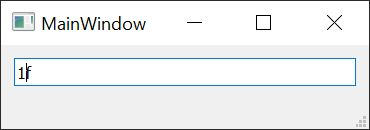
\includegraphics[scale=0.5]{Figures/edit4.jpg}}
  }
  \\
  {}
  &{
  \boxed{
    \textbf{Controller}
  }
  }
  &{}
}
\]
Обратите внимание, что модель в этом случае не просто строка, а строка и позиция курсора.
Потому что окно для редактирования умеет показывать положение курсора для редактирования.
Логически данные (или состояние) хранится только в модели.
View ничего не хранит (логически не хранит, всякое кэширование данных и прочие вспомогательные структуры могут использоваться).
Важно, что только данные из модели являются настоящей правдой.
То есть без модели View не знает что рисовать.
У нее нет дефолтного состояния.
Контроллер -- это просто кусок кода, который принимает команды от пользователя и на основе них вызывает методы у модели.

\paragraph{Виды соединений}

Теперь когда у нас есть три компоненты надо понять как они друг с другом связаны.
Бывают два типа соединения:
\begin{center}
\begin{tabular}{cc}
{
$
\xymatrix{
  {\phantom{\text{Model}}}
  {\save
  [].[dd]*+[F--]\frm{}
  \restore
  } 
  &{\text{View1}}\\
  {\text{Model}}\ar@{-->}[ru]\ar@{-->}[r]\ar@{-->}[rd]&{\text{View2}}\\
  {}&{\text{View3}}\\
}
$
}
&
{
$
\xymatrix{
  {\text{Controller1}}\ar@{->>}[rd]&  {\phantom{\text{Model}}}
  {\save
  [].[dd]*+[F--]\frm{}
  \restore
  }
  \\
  {\text{Controller2}}\ar@{->>}[r]&{\text{Model}}\\
  {\text{Controller3}}\ar@{->>}[ru]&{}\\
}
$
}\vspace{0.5cm}\\
{
$
\xymatrix{
  {\text{Observable}}\ar@{-->}[r]&{\text{Observer}}
}
$
}
&
{
$
\xymatrix{
  {\text{Controller}}\ar@{->>}[r]&{\text{Model}}
}
$
}
\end{tabular}
\end{center}
Соединение представленное слева -- это push уведомления, которые представляют из себя Observalbe/Observer соединения, которое обсуждалось в разделе~\ref{section::Observer}.
Его главная особенность в том, что у нас один источник данных и много слушателей для этих данных.
Соединение справа -- это соединение Host/Handle, которое обсуждалось в разделе~\ref{section::TrackingPtr}.
Его основная особенность, что наоборот может быть много контроллеров на одну модель.

\subsubsection{Модель для MVC}

\paragraph{Обычная модель}

Обычно принято рисовать такую общую картинку для описания того, как соединяются компоненты между собой.
\[
\xymatrix{
  {\phantom{\text{Model}}}
  {\save
  [].[dd]*+[F--]\frm{}
  \restore
  }  
  &{\text{View}}\ar@{-->}[dd]\\
  {\text{Model}}\ar@{-->}[ru]&{}\\
  {}&{\text{Controller}}\ar@{->>}[lu]\\
}
\]
Пунктиром тут обозначены границы ядра программы.
Эта часть вообще не зависит ни от каких графических библиотек.
Эта часть даже не знает, что она является частью интерактивного приложения.
\begin{itemize}
\item
Модель внутри ядра -- основной источник данных.
Как только View присоединилась к Model, то Model тут же отправляет ей свое текущее состояние и View тут же его отрисовывает таким, какое оно есть.
Если у модели что-то поменялось, то она тут же оповещает свою View (или несколько View), чтобы та отобразила ее в текущем состоянии.
К одной модели может быть подсоединено много разных View.
Вы можете пытаться отображать данные в разных форматах в разных окнах или вообще принципиально разных способом.

\item
Контроллер же наоборот управляет моделью по указателю.
Точнее, чтобы соединение было надежным это надо делать через handle.
В данном случае Model является host.
А внутри контроллера содержится handle для управления моделью.
У одной модели может быть много контроллеров.
Например, один контроллер от клавиатуры, а другой от GUI.
Потому тут не подходит Observable/Observer соединение.

\item
И последняя часть -- соединение между View и Controller.
Обычно представляют, что это тоже push уведомления по типу Observer/Observable.
Почему это так.
Ну потому что если пользователь нажал на кнопку экрана, то это возникло какое-то действие, о котором знает View.
И значит она должна сообщить теперь об этом Controller.
Однако так бывает не всегда.
Бывает что источник сигнала не внутри View.
Например ввод с клавиатуры.
\end{itemize}
Когда вы пишите свое интерактивное приложение, вы вряд ли пишите все GUI и Message Driven System-у с нуля сами, вы скорее всего используете готовые решения.
А тогда есть подозрения, что ни одна из библиотек не поддерживает возможности соединяться по Observable/Observer соединению, в особенности используемому вами в вашем проекте.
Потому полезно эту концептуальную картину немного представить в другом виде.

\paragraph{Другая модель}

Вот еще чуть более реалистичная картинка.
\[
\xymatrix{
  {\phantom{\text{Model}}}
  {\save
  [].[dd]*+[F--]\frm{}
  \restore
  }  
  &{\text{View}}\ar[r]&{\text{GUI}}
  {\save
  [].[dd]*+[F--]\frm{}
  \restore
  }\\
  {\text{Model}}\ar@{-->}[ru]&{}&{\text{Library}}\\
  {}&{\text{Controller}}\ar@{->>}[lu]&{\text{Message System}}\ar@{~>}[l]\\
}
\]
Здесь виды соединений:
\[
\xymatrix@R=5pt@C=15pt{
  {\text{Observable}(1)}\ar@{-->}[r]&{\text{Observer}(n)}&  {\text{View}(1)}\ar@{->}[r]&{\text{GUI}(1)}\\
  {\text{Controller}(n)}\ar@{->>}[r]&{\text{Model}(1)}&  {\text{Message System}(1)}\ar@{~>}[r]&{\text{Controller}(n)}\\
}
\]
Давайте прокомментируем соединения.
\begin{enumerate}
\item Model$\to$View -- как и раньше Observable/Observer соединение для поставления данных из модели во View.
Соединение от одной модели к многим View.

\item Controller$\to$Model -- как и раньше соединение по типу Host/Handle для управления моделью.
Соединение от нескольких контроллеров к одной модели.

\item View$\to$GUI.
Если вы используете готовую GUI библиотеку, то для каждого View объекта вы будете использовать библиотечный код для имплементации GUI.
Обычно для одной View вы создаете один объект, представляющей состояние View (состояние графического изображения для пользователя, но НЕ состояние модели).
Это обычно один в один соединение.

\item Message System$\to$Controller.
В интерактивных приложениях обычно используются Message Driven Systems, которые обсуждались в разделе~\ref{section::MDS}.
Любые действия пользователя тогда перерабатываются в сообщения системы.
А потому контроллер должен прослушивать данные сообщения и после этого совершать нужные действия с моделью.
Тут есть такая тонкость.
Все ли необходимые для совершения действия данные прилетают внутри сообщения.
Бывает так, что не все.
А тогда у контроллера должна быть возможность эти данные получить.
А это значит, что он может хранить какие-то указатели или лучше handle-ы на графические компоненты, где должны быть данные.
\end{enumerate}

\subsubsection{Демонстрация как работает MVC}

Давайте вернемся к первой модели в маленьком масштабе из предыдущего примера.
Напомню, что у нас есть простое окно с полем для ввода и изменения текста.
Предположим, что мы поставили курсор и нажали друг за другом клавиши <<1>>, <<f>> и <<$\leftarrow$>>.
Тогда видимое еоведение будет таким
\[
\xymatrix@R=40pt@C=50pt{
  {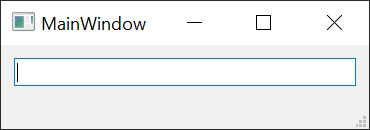
\includegraphics[scale=0.5]{Figures/edit1.jpg}}
  \ar@{|->}[r]^{\boxed{1}}
  &
  {{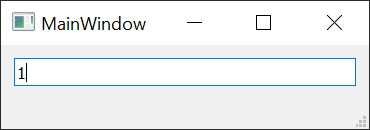
\includegraphics[scale=0.5]{Figures/edit2.jpg}}}
  \ar@{|->}[dl]+(-2,11)|{\boxed{f}}
  \\
  {{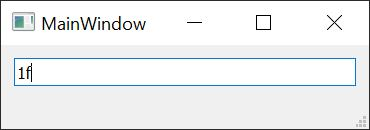
\includegraphics[scale=0.5]{Figures/edit3.jpg}}}
  \ar@{|->}[r]^{\boxed{\leftarrow}}
  &
  {{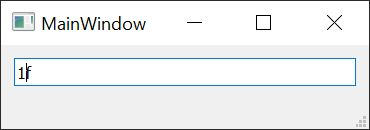
\includegraphics[scale=0.5]{Figures/edit4.jpg}}}
}
\]
Давайте посмотрим, как такая система должна работать по внутренней логике MVC паттерна.
У любой интерактивной программы есть две стадии:
\begin{enumerate}
\item Инициализация всех ресурсов для начала исполнения.

\item Исполнение программы.
\end{enumerate}
Во время первой стадии нам нужно проделать следующее:
\begin{enumerate}
\item Создать Model.

\item Создать View.

\item Создать Controller.

\item Соединить Model$\to$View.

\item Соединить View$\to$Controller.

\item Соединить Controller$\to$Model.
\end{enumerate}
Во время второй стадии собранная система реагирует на сообщения Message Driven System-ы.

Начнем с создания объектов.
В конструкторе нашего приложения мы создаем Model, View и Controller.
Логически будем представлять их так.
\[
\xymatrix{
  {
  \boxed{
  \begin{tabular}{c}
    string:\;""\\
    int:\;0
  \end{tabular}
  }
  }
  %\ar@{-->}[rr]
  &{}&
  {
  \parbox{3cm}{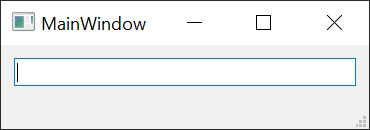
\includegraphics[scale=0.5]{Figures/edit1.jpg}}
  }
  %\ar@{-->}[dl]
  \\
  {}&
  {
  {\boxed{
    \text{Ctrl}
  }}
  }
  %\ar@{->>}[ul]
  &{}
}
\]
Обратите внимание, что сейчас у меня показывается окно с пустым полем для ввода и позицией коретки на нуле.
Однако, это не очень правильное представление.
По хорошему в этом состоянии View просто показывает белое поле без информации.
View лишь знает геометрию поля для ввода, но не его содержание.
И лишь в момент соединения Model и View, данные от модели поступают во View и она их отрисовывает.
\[
\xymatrix{
  {
  \boxed{
  \begin{tabular}{c}
    string:\;""\\
    int:\;0
  \end{tabular}
  }
  }
  \ar@{-->}[rr]^{\text{Оповещение}}
  &{}&
  {
  \parbox{3cm}{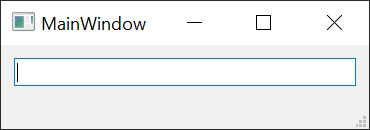
\includegraphics[scale=0.5]{Figures/edit1.jpg}}
  }
  %\ar@{-->}[dl]
  \\
  {}&
  {
  {\boxed{
    \text{Ctrl}
  }}
  }
  %\ar@{->>}[ul]
  &{}
}
\]
Полностью собранная схема будет выглядеть так
\[
\xymatrix{
  {
  \boxed{
  \begin{tabular}{c}
    string:\;""\\
    int:\;0
  \end{tabular}
  }
  }
  \ar@{-->}[rr]
  &{}&
  {
  \parbox{3cm}{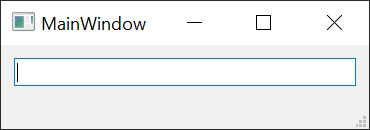
\includegraphics[scale=0.5]{Figures/edit1.jpg}}
  }
  \ar@{-->}[dl]
  \\
  {}&
  {
  \boxed{
    \text{Ctrl}
  }
  }
  \ar@{->>}[ul]
  &{}
}
\]
На этом закончилась стадия конструирования.
Перейдем к стадии обработки сообщений.
На этой стадии мы считаем, что пользователь последовательно выполнил следующие команды
\begin{enumerate}
\item Нажата клавиша <<1>>.

\item Нажата клавиша <<f>>.

\item Нажата клавиша <<$\leftarrow$>> (стрелка влево).
\end{enumerate}
Ниже показана поэтапная схема, отражающая, что происходит в MVC контуре.
Красным обозначается текущая в данный момент операция.
\begin{center}
\newcounter{listitem}
\newcommand{\listitem}{\par\addtocounter{listitem}{1}\noindent\textbf{\arabic{listitem})}\; }
\begin{longtable}{ll}
{
\listitem
\begin{minipage}[\baselineskip]{8cm}
\[
\xymatrix{
  {
  \boxed{
  \begin{tabular}{c}
    string:\;``''\\
    int:\;0
  \end{tabular}
  }
  }
  \ar@{-->}[rr]
  &{}
  &{
  \parbox{3cm}{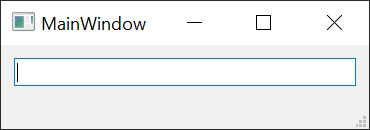
\includegraphics[scale=0.45]{Figures/edit1.jpg}}
  }
  \ar@{-->}@[red][dl]|-{\boxed{1}}
  \\
  {}
  &{
  \boxed{
    \text{Ctrl}
  }
  }
  \ar@{->>}[ul]
  &{}
}
\]
\end{minipage}
}&{
\listitem
\begin{minipage}[\baselineskip]{8cm}
\[
\xymatrix{
  {
  \boxed{
  \begin{tabular}{c}
    string:\;``''\\
    int:\;0
  \end{tabular}
  }
  }
  \ar@{-->}[rr]
  &{}
  &{
  \parbox{3cm}{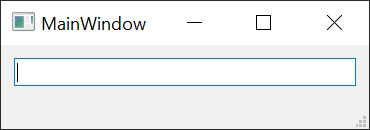
\includegraphics[scale=0.45]{Figures/edit1.jpg}}
  }
  \ar@{-->}[dl]
  \\
  {}
  &{
  \boxed{
    \text{Ctrl}
  }
  }
  \ar@{->>}@[red][ul]
  &{}
}
\]
\end{minipage}
}\\\hline
{
\listitem
\begin{minipage}[\baselineskip]{8cm}
\[
\xymatrix{
  {
  \boxed{
  \begin{tabular}{c}
    string:\;\color{red}{``1''}\\
    int:\;\color{red}{1}
  \end{tabular}
  }
  }
  \ar@{-->}[rr]
  &{}
  &{
  \parbox{3cm}{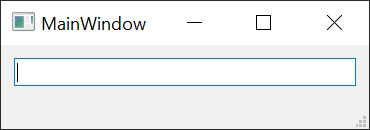
\includegraphics[scale=0.45]{Figures/edit1.jpg}}
  }
  \ar@{-->}[dl]
  \\
  {}
  &{
  \boxed{
    \text{Ctrl}
  }
  }
  \ar@{->>}[ul]
  &{}
}
\]
\end{minipage}
}&{
\listitem
\begin{minipage}[\baselineskip]{8cm}
\[
\xymatrix{
  {
  \boxed{
  \begin{tabular}{c}
    string:\;``1''\\
    int:\;1
  \end{tabular}
  }
  }
  \ar@{-->}@[red][rr]
  &{}
  &{
  \parbox{3cm}{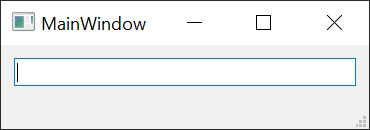
\includegraphics[scale=0.45]{Figures/edit1.jpg}}
  }
  \ar@{-->}[dl]
  \\
  {}
  &{
  \boxed{
    \text{Ctrl}
  }
  }
  \ar@{->>}[ul]
  &{}
}
\]
\end{minipage}
}\\\hline
{
\listitem
\begin{minipage}[\baselineskip]{8cm}
\[
\xymatrix{
  {
  \boxed{
  \begin{tabular}{c}
    string:\;``1''\\
    int:\;1
  \end{tabular}
  }
  }
  \ar@{-->}[rr]
  &{}
  &{
  \parbox{3cm}{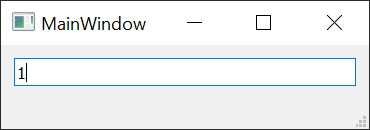
\includegraphics[scale=0.45]{Figures/edit2.jpg}}
  }
  \ar@{-->}[dl]
  \\
  {}
  &{
  \boxed{
    \text{Ctrl}
  }
  }
  \ar@{->>}[ul]
  &{}
}
\]
\end{minipage}
}&{
\listitem
\begin{minipage}[\baselineskip]{8cm}
\[
\xymatrix{
  {
  \boxed{
  \begin{tabular}{c}
    string:\;``1''\\
    int:\;1
  \end{tabular}
  }
  }
  \ar@{-->}[rr]
  &{}
  &{
  \parbox{3cm}{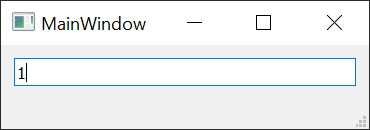
\includegraphics[scale=0.45]{Figures/edit2.jpg}}
  }
  \ar@{-->}@[red][dl]|-{\boxed{f}}
  \\
  {}
  &{
  \boxed{
    \text{Ctrl}
  }
  }
  \ar@{->>}[ul]
  &{}
}
\]
\end{minipage}
}\\\hline
{
\listitem
\begin{minipage}[\baselineskip]{8cm}
\[
\xymatrix{
  {
  \boxed{
  \begin{tabular}{c}
    string:\;``1''\\
    int:\;1
  \end{tabular}
  }
  }
  \ar@{-->}[rr]
  &{}
  &{
  \parbox{3cm}{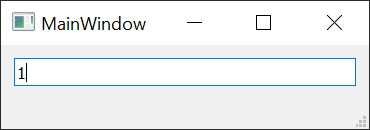
\includegraphics[scale=0.45]{Figures/edit2.jpg}}
  }
  \ar@{-->}[dl]
  \\
  {}
  &{
  \boxed{
    \text{Ctrl}
  }
  }
  \ar@{->>}@[red][ul]
  &{}
}
\]
\end{minipage}
}&{
\listitem
\begin{minipage}[\baselineskip]{8cm}
\[
\xymatrix{
  {
  \boxed{
  \begin{tabular}{c}
    string:\;\color{red}{``1f''}\\
    int:\;\color{red}{2}
  \end{tabular}
  }
  }
  \ar@{-->}[rr]
  &{}
  &{
  \parbox{3cm}{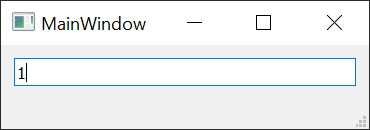
\includegraphics[scale=0.45]{Figures/edit2.jpg}}
  }
  \ar@{-->}[dl]
  \\
  {}
  &{
  \boxed{
    \text{Ctrl}
  }
  }
  \ar@{->>}[ul]
  &{}
}
\]
\end{minipage}
}\\\hline
{
\listitem
\begin{minipage}[\baselineskip]{8cm}
\[
\xymatrix{
  {
  \boxed{
  \begin{tabular}{c}
    string:\;``1f''\\
    int:\;2
  \end{tabular}
  }
  }
  \ar@{-->}@[red][rr]
  &{}
  &{
  \parbox{3cm}{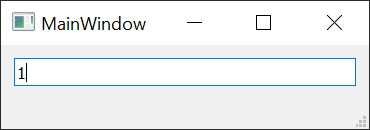
\includegraphics[scale=0.45]{Figures/edit2.jpg}}
  }
  \ar@{-->}[dl]
  \\
  {}
  &{
  \boxed{
    \text{Ctrl}
  }
  }
  \ar@{->>}[ul]
  &{}
}
\]
\end{minipage}
}&{
\listitem
\begin{minipage}[\baselineskip]{8cm}
\[
\xymatrix{
  {
  \boxed{
  \begin{tabular}{c}
    string:\;``1f''\\
    int:\;2
  \end{tabular}
  }
  }
  \ar@{-->}[rr]
  &{}
  &{
  \parbox{3cm}{\includegraphics[scale=0.45]{Figures/edit3.jpg}}
  }
  \ar@{-->}[dl]
  \\
  {}
  &{
  \boxed{
    \text{Ctrl}
  }
  }
  \ar@{->>}[ul]
  &{}
}
\]
\end{minipage}
}\\\hline
{
\listitem
\begin{minipage}[\baselineskip]{8cm}
\[
\xymatrix{
  {
  \boxed{
  \begin{tabular}{c}
    string:\;``1f''\\
    int:\;2
  \end{tabular}
  }
  }
  \ar@{-->}[rr]
  &{}
  &{
  \parbox{3cm}{\includegraphics[scale=0.45]{Figures/edit3.jpg}}
  }
  \ar@{-->}@[red][dl]|-{\boxed{\leftarrow}}
  \\
  {}
  &{
  \boxed{
    \text{Ctrl}
  }
  }
  \ar@{->>}[ul]
  &{}
}
\]
\end{minipage}
}&{
\listitem
\begin{minipage}[\baselineskip]{8cm}
\[
\xymatrix{
  {
  \boxed{
  \begin{tabular}{c}
    string:\;``1f''\\
    int:\;2
  \end{tabular}
  }
  }
  \ar@{-->}[rr]
  &{}
  &{
  \parbox{3cm}{\includegraphics[scale=0.45]{Figures/edit3.jpg}}
  }
  \ar@{-->}[dl]
  \\
  {}
  &{
  \boxed{
    \text{Ctrl}
  }
  }
  \ar@{->>}@[red][ul]
  &{}
}
\]
\end{minipage}
}\\\hline
{
\listitem
\begin{minipage}[\baselineskip]{8cm}
\[
\xymatrix{
  {
  \boxed{
  \begin{tabular}{c}
    string:\;``1f''\\
    int:\;\color{red}{1}
  \end{tabular}
  }
  }
  \ar@{-->}[rr]
  &{}
  &{
  \parbox{3cm}{\includegraphics[scale=0.45]{Figures/edit3.jpg}}
  }
  \ar@{-->}[dl]
  \\
  {}
  &{
  \boxed{
    \text{Ctrl}
  }
  }
  \ar@{->>}[ul]
  &{}
}
\]
\end{minipage}
}&{
\listitem
\begin{minipage}[\baselineskip]{8cm}
\[
\xymatrix{
  {
  \boxed{
  \begin{tabular}{c}
    string:\;``1f''\\
    int:\;1
  \end{tabular}
  }
  }
  \ar@{-->}@[red][rr]
  &{}
  &{
  \parbox{3cm}{\includegraphics[scale=0.45]{Figures/edit3.jpg}}
  }
  \ar@{-->}[dl]
  \\
  {}
  &{
  \boxed{
    \text{Ctrl}
  }
  }
  \ar@{->>}[ul]
  &{}
}
\]
\end{minipage}
}\\\hline
{
\listitem
\begin{minipage}[\baselineskip]{8cm}
\[
\xymatrix{
  {
  \boxed{
  \begin{tabular}{c}
    string:\;``1f''\\
    int:\;1
  \end{tabular}
  }
  }
  \ar@{-->}[rr]
  &{}
  &{
  \parbox{3cm}{\includegraphics[scale=0.45]{Figures/edit4.jpg}}
  }
  \ar@{-->}[dl]
  \\
  {}
  &{
  \boxed{
    \text{Ctrl}
  }
  }
  \ar@{->>}[ul]
  &{}
}
\]
\end{minipage}
}&{
}\\
\end{longtable}
\end{center}
Давайте прокомментируем как это работает.
\begin{enumerate}
\item После нажатия на клавишу <<1>> оповещается соответствующий графический компонент, в нашем случае это поле для ввода текста.
В этот момент поле ввода для текста НЕ меняется, потому что у него нет внутреннего состояния, оно всегда отражает состояние модели.
Вместо этого этот компонент посылает сообщение контроллеру, что нажата клавиша <<1>>.

\item На этом этапе контроллер видит, что клавиша <<1>> дает символ ``1'', который надо поместить в строку внутри модели и сдвинуть коретку на $1$ вперед.

\item На этом слайде красным помечено изменение состояния модели.

\item Как только модель изменила свое состояние, она оповещает всех, кто на нее подписан, чтобы они пришли с ней в одно состояние.
В частности оповещается поле для ввода текста о новом состоянии модели.

\item И вот на этом шаге поле для ввода текста получив новое состояние модели отражает его в виде строки <<1>> и положения картки после цифры $1$.

\item После нажатия на клавишу <<f>>, оповещается графически элемент -- поле для ввода текста.
После чего это поле посылает сигнал контроллеру.

\item Контроллер видит, что эта клавиша дает символ.
И зовет метод модели, который добавляет этот символ в месте расположения каретки.

\item Здесь красным обозначено новое состояние модели.
Теперь хранится строка <<1f>> и новое положение каретки $2$.

\item Теперь модель оповещает текстовое поле о своем новом состоянии.

\item Текстовое поле отражает новое состояние модели.
То есть оно отображает строку <<1f>> и новое положение коретки в конце строки.

\item Теперь после нажатия пользователем клавишы <<$\leftarrow$>> -- стрелка влево, оповещается соответствующий графический компонент -- поле ввода для текста.
Этот компонент посылает сигнал контроллеру.

\item Контроллер видит, что это клавиша отвечает за навигацию по тексту и вызывает у модели метод сдвига коретки влево.

\item Новое положение коретки в модели отмечено красным.
Строка не меняется.

\item Теперь модель оповещает всех о своем новом состоянии.

\item И наконец-то текстовое поле отображает текущую строку <<1f>> и положение коретки между этих двух символов.
\end{enumerate}
Этот пример хорошо показывает общую логику работы MVC.
Все данные хранятся в модели, она единственный источник информации.
View всегда отражает только то, что ей прилетело от модели и логически не имеет своего состояния.
Контроллер же управляет моделью напрямую.

\paragraph{Замечание про Controller}

В такой схеме может показаться странным, что нам нужно использовать View и Controller как две разные сущности.
Потому что все равно все данные из View идут в Controller и потом по этим данным дергается модель.
Причина почему выделяется контроллер -- мы не хотим, чтобы в GUI коде была бизнес логика управления моделью.
Мы не хотим, чтобы GUI зависело от ядра.
Мы хотим, чтобы GUI зависило от данных, которые прилетают из ядра по Observer паттерну, но мы не хотим чтобы были какие-либо другие зависимости.
Чтобы отрезать GUI код от ядра и вводится контроллер.
В этом случае View лишь зависит от двух типов данных: получаемые от модели и отсылаемые контроллеру.
View не принимает никаких решений, не умеет управлять моделью, не содержит никакой логики.
Вся логика управления уходит в Controller.

\subsubsection{MVC и реальность}

Если вы работаете с готовыми графическими библиотеками, то к сожалению или к счастью, они не предоставляют stateless (без состояния) графических компонент (или не всегда их предоставляют).
А потому любой графический компонент или widget в реальной библиотеки сам из себя представляет уже готовый MVC контур запеченый в один объект.
И если вы пытаетесь использовать этот widget как View, у вас получится какая-то такая картинка:
\[
\xymatrix{
  {}&{}&{}&{\text{\textbf{Widget}}}&{}\\
  {}&{}&{\text{M}}\ar@{-->}[rr]
  {\save
  [].[rrd]*+[F-]\frm{}
  \restore
  }
  &{}&{\text{V}}\ar@{-->}[dl]\\
  {\text{Model}}\ar@{-->}@(u,l)[urr]&{}&{}\ar@{-->}@(d,r)[dl]&{\text{C}}\ar@{->>}[ul]&{}\\
  {}&{\text{Ctrl}}\ar@{->>}@(l,d)[ul]&{}&{}&{}\\
}
\]
В бокс справа на картинке объединены внутренности Widget.
При использовании View, которая имеет состояние, вы по сути имеете две модели, которые вам придется согласовывать.
А согласование двух моделей при двустороннем общении -- это всегда огромная проблема.
У вас возникают следующие проблемы
\begin{enumerate}
\item Двойное обновление модели.

\item Гашение обратной связи.
\end{enumerate}
Давайте промоделируем одно оповещение контроллера в схеме представленной выше.
Предположим на пользователь совершил какое-то действие, которое заставило View внутри Widget-а оповестить контроллер внутри Widget-а.
\begin{center}
\setcounter{listitem}{0}
\newcommand{\listitem}{\par\addtocounter{listitem}{1}\noindent\textbf{\arabic{listitem})}\; }
\begin{longtable}{ll}
{
\listitem
\begin{minipage}[\baselineskip]{8cm}
\[
\xymatrix@R=15pt@C=15pt{
  {}&{}&{}&{\textbf{Qt Widget}}&{}\\
  {}&{}&{\text{M}}\ar@{-->}[rr]
  {\save
  [].[rrd]*+[F-]\frm{}
  \restore
  }
  &{}&{\text{V}}\ar@{-->}@[red][dl]\\
  {\text{Model}}\ar@{-->}@(u,l)[urr]&{}&{}\ar@{-->}@(d,r)[dl]&{\text{C}}\ar@{->>}[ul]&{}\\
  {}&{\text{Ctrl}}\ar@{->>}@(l,d)[ul]&{}&{}&{}\\
}
\]
\end{minipage}
}&{
\listitem
\begin{minipage}[\baselineskip]{8cm}
\[
\xymatrix@R=15pt@C=15pt{
  {}&{}&{}&{\textbf{Qt Widget}}&{}\\
  {}&{}&{\text{M}}\ar@{-->}[rr]
  {\save
  [].[rrd]*+[F-]\frm{}
  \restore
  }
  &{}&{\text{V}}\ar@{-->}[dl]\\
  {\text{Model}}\ar@{-->}@(u,l)[urr]&{}&{}\ar@{-->}@(d,r)[dl]&{\text{C}}\ar@{->>}@[red][ul]&{}\\
  {}&{\text{Ctrl}}\ar@{->>}@(l,d)[ul]&{}&{}&{}\\
}
\]
\end{minipage}
}\\\hline
{
\listitem
\begin{minipage}[\baselineskip]{8cm}
\[
\xymatrix@R=15pt@C=15pt{
  {}&{}&{}&{\textbf{Qt Widget}}&{}\\
  {}&{}&{\text{M}}\ar@{-->}@[red][rr]
  {\save
  [].[rrd]*+[F-]\frm{}
  \restore
  }
  &{}&{\text{V}}\ar@{-->}[dl]\\
  {\text{Model}}\ar@{-->}@(u,l)[urr]&{}&{}\ar@{-->}@(d,r)[dl]&{\text{C}}\ar@{->>}[ul]&{}\\
  {}&{\text{Ctrl}}\ar@{->>}@(l,d)[ul]&{}&{}&{}\\
}
\]
\end{minipage}
}&{
\listitem
\begin{minipage}[\baselineskip]{8cm}
\[
\xymatrix@R=15pt@C=15pt{
  {}&{}&{}&{\textbf{Qt Widget}}&{}\\
  {}&{}&{\text{M}}\ar@{-->}[rr]
  {\save
  [].[rrd]*+[F-]\frm{}
  \restore
  }
  &{}&{\text{V}}\ar@{-->}[dl]\\
  {\text{Model}}\ar@{-->}@(u,l)[urr]&{}&{}\ar@{-->}@(d,r)@[red][dl]&{\text{C}}\ar@{->>}[ul]&{}\\
  {}&{\text{Ctrl}}\ar@{->>}@(l,d)[ul]&{}&{}&{}\\
}
\]
\end{minipage}
}\\\hline
{
\listitem
\begin{minipage}[\baselineskip]{8cm}
\[
\xymatrix@R=15pt@C=15pt{
  {}&{}&{}&{\textbf{Qt Widget}}&{}\\
  {}&{}&{\text{M}}\ar@{-->}[rr]
  {\save
  [].[rrd]*+[F-]\frm{}
  \restore
  }
  &{}&{\text{V}}\ar@{-->}[dl]\\
  {\text{Model}}\ar@{-->}@(u,l)[urr]&{}&{}\ar@{-->}@(d,r)[dl]&{\text{C}}\ar@{->>}[ul]&{}\\
  {}&{\text{Ctrl}}\ar@{->>}@(l,d)@[red][ul]&{}&{}&{}\\
}
\]
\end{minipage}
}&{
\listitem
\begin{minipage}[\baselineskip]{8cm}
\[
\xymatrix@R=15pt@C=15pt{
  {}&{}&{}&{\textbf{Qt Widget}}&{}\\
  {}&{}&{\text{M}}\ar@{-->}[rr]
  {\save
  [].[rrd]*+[F-]\frm{}
  \restore
  }
  &{}&{\text{V}}\ar@{-->}[dl]\\
  {\text{Model}}\ar@{-->}@(u,l)@[red][urr]&{}&{}\ar@{-->}@(d,r)[dl]&{\text{C}}\ar@{->>}[ul]&{}\\
  {}&{\text{Ctrl}}\ar@{->>}@(l,d)[ul]&{}&{}&{}\\
}
\]
\end{minipage}
}\\\hline
{
\listitem
\begin{minipage}[\baselineskip]{8cm}
\[
\xymatrix@R=15pt@C=15pt{
  {}&{}&{}&{\textbf{Qt Widget}}&{}\\
  {}&{}&{\text{M}}\ar@{-->}@[red][rr]
  {\save
  [].[rrd]*+[F-]\frm{}
  \restore
  }
  &{}&{\text{V}}\ar@{-->}[dl]\\
  {\text{Model}}\ar@{-->}@(u,l)[urr]&{}&{}\ar@{-->}@(d,r)[dl]&{\text{C}}\ar@{->>}[ul]&{}\\
  {}&{\text{Ctrl}}\ar@{->>}@(l,d)[ul]&{}&{}&{}\\
}
\]
\end{minipage}
}&{
\listitem
\begin{minipage}[\baselineskip]{8cm}
\[
\xymatrix@R=15pt@C=15pt{
  {}&{}&{}&{\textbf{Qt Widget}}&{}\\
  {}&{}&{\color{red}{\text{M}}}\ar@{-->}[rr]
  {\save
  [].[rrd]*+[F-]\frm{}
  \restore
  }
  &{}&{\text{V}}\ar@{-->}[dl]\\
  {\color{red}{\text{Model}}}\ar@{-->}@(u,l)@[red][urr]&{}&{}\ar@{-->}@(d,r)[dl]&{\text{C}}\ar@{->>}[ul]&{}\\
  {}&{\text{Ctrl}}\ar@{->>}@(l,d)[ul]&{}&{}&{}\\
}
\]
\end{minipage}
}\\
\end{longtable}
\end{center}
Давайте прокомментируем, что тут происходит.
Если мы верим, что Widget функционирует как MVC контур (раз он содержит состояние), то мы ожидаем следующее поведение.
\begin{enumerate}
\item В начале Widget получает от экосистемы сообщение о действиях пользователя.
А именно View объект внутри Widget-а оповещается об этом событии.
После чего View объект должен оповестить внутренний контроллер, чтобы обновить свое состояние.

\item Когда внутренний контроллер получает оповещение, он дергает внутреннюю модель, чтобы она обновилась.

\item Когда модель обновилась она совершает два действия.
Первое -- оно оповещает внутренний View объект, чтобы отразить свое новое состояние.

\item Второе действие -- послать сигнал наружним объектам.
В данном случае внешнему контроллеру Ctrl.

\item Теперь контроллер оповещает нашу модель Model.

\item Модель меняет свое состояние и оповещает Widget.

\item Widget меняет состояние внутренней модели в соответствии с состоянием, которое пришло от Model.
А раз обновилось внутреннее состояние, то надо опять оповестить внутренюю View.

\item Как мы видим, в ребре между двумя моделями оказалось, двойное обновление внутренней модели одними и теми же данными.
Из-за чего происходит двойное обновление View внутри Widget.
Эта проблема связана с тем, что модель снаружи и внутри Widget общаются в двустороннем порядке.
\end{enumerate}
Поведение описанное выше может быть как желательным, так и не желательным.
Например, если мы использовали statefull Widget мы не хотим двойное обновление View объекта, чтобы экран лишний раз не мерцал.
Ну и в целом это логически плохо.

Какие есть методы решения этой проблемы.
\begin{enumerate}
\item Одно из частных решений -- поставить гаситель обратной связи или Suppressor на стороне M.
Это значит, что когда мы оповещаем всех, мы перестаем слушать входящие сигналы.
К сожалению это работает только для блокирующих вызовов.
Кроме того, может быть опасность пропустить нужный сигнал от модели.

\item Другой подход -- поместить некую логику оповещения на стороне Model.
То есть теперь Model должна знать кого оповещать а кого нет.
Это достаточно сложная задача, потому что контроллеру надо передавать модели данные об отправители и Model теперь должна не просто обновлять свое состояние, но еще и принимать решение кого оповещать.
Это опасно рассинхроном состояний.

\item Можно поместить логику обработки оповещений на стороне внутренней модели M.
То есть внутренняя модель смотри прилетевшие данные и проверяет отличается ли ее состояние от пришедшего.
Это логически самое правильное решение, но тогда нам надо уметь очень быстро считать разницу между состояниями.
Иначе этот подход может оказаться очень дорогим для исполнения.
\end{enumerate}
На удивление все становится сильно проще и удобнее, если мы переходим к неблокирующим соединениям между компонентами.
В данном случае неблокирующий observer паттерн (можно посмотреть раздел~\ref{section::ObserverNonBlocking}).
В этом случае общение компонент можно рассматривать как общение по сети.
И для корректного общения нужен грамотный протокол общения, который решает все проблемы подобного характера.
Никакие кустарные заплатки в виде suppressor-ов в нем не потребуются.

\subsubsection{Пример 1 использования MVC}

Здесь я хочу привести пример программы по анализу качества печати, которую я разрабатывал.
Начну со скриншота, чтобы можно было что-то объяснять.
\begin{center}
\includegraphics[scale=0.355]{Figures/appfull.JPG}
\end{center}
Давайте в общих чертах объясню, что здесь происходит.
Данная программа представляет из себя всего одно окно, которое вы видите на скриншоте выше.
Программа умеет находиться в двух режимах:
\begin{enumerate}
\item Режим перехвата клавиватуры.
В свернутом режиме, программа перехватывает весь ввод пользователя.

\item Режим анализа.
В развернутом режиме, программе не прослушивает клавиатуру, вместо этого она дает возможность посмотреть информацию о уже записанных данных, которые были перехвачены ранее.
\end{enumerate}
При переходе от прослушивающего состояния в состояние анализа все накопленные данные сгружаются в ядро программы.
Вся информация о наборе хранится в виде сессий.
Теперь опишем компоненты графического интерфейса.
\begin{enumerate}
\item
Слева вы видите список сессий, где отражено несколько первых клавиш нажатых в данную сессию, ее длина в количестве нажатых клавиш и какая сессия сейчас активна.
\begin{center}
\includegraphics[scale=0.5]{Figures/SessView.JPG}
\end{center}

\item Над панелью для выбора сессий находится панель выбора режима для отображения перехваченного набора.
\begin{center}
\includegraphics[scale=0.5]{Figures/textmodev.JPG}
\end{center}
Данный режим влияет на отображение сессии в текстовом окне описанном в пункте~\ref{item::TextView}.
Есть три режима
\begin{enumerate}
\item Сырой.
В нем отображаются все клавиши которые были нажаты независимо от того дают они символы или нет.

\item Полный.
В этом режиме отображаются только напечатанные символы включая все удаленные.
Удаленные символы подсвечиваются специальным образом.

\item Напечатанный.
В этом режиме отображается только конечный текст, который был напечатан без учета стертых символов.
\end{enumerate}

\item
\label{item::TextView}
Сверху по центру расположено текстовое окно предоставляющее информацию о перехваченной сессии.
\begin{center}
\includegraphics[scale=0.5]{Figures/TextView.JPG}
\end{center}

\item Ниже идет график плотности скорости.
\begin{center}
\includegraphics[scale=0.5]{Figures/plotView.JPG}
\end{center} 
Программа трактует скорость нажатия клавиши как случайную величину.
В данном окне приведена плотность распределения данной случайной величины.

\item Справа от текстового окна располагается окно статистики.
\begin{center}
\includegraphics[scale=0.5]{Figures/StatView.JPG}
\end{center}
Самый интересный параметр -- предпоследний параметр -- это пик плотности распределения скорости.
Этот параметр хорошо характеризует скорость физических возможностей наборщика.

\item В самом низу находится клавишная схема, на которой отображается каким пальцем какая клавиша и в какой временной промежуток была нажата.
\begin{center}
\includegraphics[scale=0.5]{Figures/DiagView.JPG}
\end{center}
\end{enumerate}
Тут стоит сказать, что от выбора текстового режима зависят: текстовое окно, график плотности и клавишная схема.
Вот пример как будет выглядеть та же самая сессия а напечатанном режиме.
\begin{center}
\includegraphics[scale=0.355]{Figures/appprint.JPG}
\end{center}
И в сыром режиме
\begin{center}
\includegraphics[scale=0.355]{Figures/appraw.JPG}
\end{center}
Видно, что в этом режиме появляются символы пробела, символы для backspace-а, для шифтов и прочие.

Давайте я продемонстрирую как выглядит часть приложения с точки зрения MVC.
\[
\resizebox{12cm}{!}{
\xymatrix@R=10pt{
  {}&{\parbox{1.5cm}{\includegraphics[scale=0.5]{Figures/SessView.JPG}}}\ar@{-->}[dl]&{}&{\parbox{1.5cm}{\includegraphics[scale=0.5]{Figures/textmodev.JPG}}}\ar@{-->}[dl]&{\parbox{3cm}{\includegraphics[scale=0.5]{Figures/TextView2.JPG}}}&{}&{\parbox{2cm}{\includegraphics[scale=0.5]{Figures/StatView.JPG}}}&{}\\
  {\text{Ctrl}}\ar@{->>}[dr]&{}&{\text{Ctrl}}\ar@{->>}[dr]&{}&{}&{}&{}&{}\\
  {}\ar@{-->}[r]&{\text{Selector}}
  {\save
  [].[rrrrd]*+[F--]\frm{}
  \restore
  }
  \ar@{-->}[rr]\ar@{-->}[uu]&{}&{\text{Text}}\ar@{-->}[d]\ar@{-->}[r]\ar@{-->}[uu]\ar@{-->}[uur]
  &{\text{Math}}\ar@{-->}[r]\ar@{-->}[rddd]+(0,9)&{\text{Stat}}\ar@{-->}[uur]&{}&{}\\
  {}&{}&{\text{Layout}}\ar@{-->}[r]&{\text{Scheme}}\ar@{-->}[ddl]+(0,9)&{}&{\phantom{\text{Plot}}}&{}&{}\\
  {}&{}&{}&{}&{}&{}&{}\\
  {\parbox{1cm}{\includegraphics[scale=0.3]{Figures/DiagView.JPG}}}&{}&{}&{}&{\makebox[0.1cm][r]{\parbox{1cm}{\includegraphics[scale=0.35]{Figures/plotView.JPG}}}}&{}&{}&{}\\
}
}
\]
Давайте я прокомментирую диаграмму выше.
\begin{itemize}
\item Часть выделенная пунктиром в центре -- это часть ядра программы.
Эта часть ничего не знает про графические библиотеки и способна работать без GUI.

\item Пунктирная стрелка слева ведет из другой части ядра, которая нам сейчас не очень важна, ибо в той части не используется MVC.

\item Ядро из себя представляет пайплайн, по которому данные проходят слева направо и после этого сообщаются пользователю через GUI.

\item Блок Selector выбирает текущую сессию для анализа.
Можно видеть MVC контур вокруг этого блока.
Selector является моделью в этом контуре.

\item Блок Text -- текстовый модуль.
Его задача хранить текущий режим и текст, который необходимо отобразить в текстовом окне.
Тут видно, что текстовое окно просто получает новые данные и через него нет возможности управления.
А выбор текстового режима -- это еще один MVC контур.

\item Блок Scheme -- модуль, который по распальцовке заданной пользователем и текущему режиму показывает диаграмму распределения нажатий по пальцам во времени.
Сама распальцовка хранится в модуле Layout и задается пользователем заранее.

\item Блок Math вычисляет плотность распределения скорости набора.
Он оповещает View отображающую плотность.

\item И в конце идет блок Stat, который является модулем статистики.
Он получает всю информацию из всех предыдущих модулей, вычисляет некую статистику и отображает ее в окне для статистики.
\end{itemize}
На этой диаграмме не отображены некоторые мелочи, как например выбор способа вычисления плотности распределения или локализация текста в элементах GUI.
Однако, я надеюсь, что эта схема хотя бы в общих чертах дает понять, как можно собирать подобное интерактивное приложение.
Так же отмечу, что все вызовы между компонентами блокирующие.
Это не очень хорошо, но это не сложно исправить имея value semantics для данных пересылаемых в observer паттерне.
Если вам интересна более детальная информация, то можно изучить \href{https://github.com/DimaTrushin/TypingAnalysis}{репозиторий} с проектом.
Там можно найти дизайн документацию с более подробным описанием происходящего.

\subsubsection{Пример 2 использования MVC}

Еще один пример, который я хочу привести -- это простая программа, которая показывает пользователю поле с двумя фишками и эти фишки можно двигать только на соседние клетки по вертикали и горизонтали.
Больше ничего делать нельзя.
Как обычно приведу скриншот в самом начале.
\begin{center}
\includegraphics[scale=0.6]{Figures/Game1.JPG}
\end{center}
Ожидаемое поведение программы такое.
Вы можете подцепить курсором фишку и перемещать ее держа зажатой левую клавишу мыши.
В момент перемещения захваченной фишки проигрывается настраиваемая анимация.
При отпускании фишки программа пытается поставить ее на указанное поле.
Если шаг сделать не возможно, то фишка возвращается в исходное состояние, откуда она была захвачена.

Важно понять, что в данном случае у нас не одна, а две модели.
\begin{enumerate}
\item Первая модель знает размер поля, расположение на нем фишек и правила, по которым фишкам можно ходить.
Эта модель оперирует целыми координатами фишек, обозначающие столбец и строку, где находится фишка.
Она ничего не знает про отображение поля, про фишки, про цвета, анимацию и прочее.
Это как бы <<внутренняя логика игры>>.

\item Вторая модель -- это геометрическая модель.
Дело в том, что в первой модели не достаточно информации для того, чтобы ее отрисовать.
Например не ясно каким цветом и как рисовать поле, какие должны быть размеры клеток, какие размеры, цвет и форма фишек.
Кроме того, при захвате фишки курсором она может находиться в состоянии, не имеющем смысла для модели игры.
Потому для отображения геометрии мы используем вторую модель.
\end{enumerate}
Схематически устройство программы выглядит так.
\[
\xymatrix{
  {\verb"model"}\ar@{-->}[rr]
  	{
	\save
   [].[]*+[F-:<3pt>]\frm{}
   \restore
	}
	{
	\save
   []+(-10,6).[drrrr]*+(3,0)++[F-:<3pt>]\frm{}
   \restore
	}
  &{}&{\verb"gmodel"}\ar@{-->}[rr]\ar@{-->}[dl]
      	{
	\save
   [].[]*+[F-:<3pt>]\frm{}
   \restore
	}
  &{}&{\verb"view"}\ar@{-->}[dl]
      	{
	\save
   [].[]*+[F-:<3pt>]\frm{}
   \restore
	}
  \\
  {}&{\verb"ctrl"}\ar@{->>}[lu]
      	{
	\save
   [].[]*+[F-]\frm{}
   \restore
	}
  &{}&{\verb"gctrl"}\ar@{->>}[lu]
      	{
	\save
   [].[]*+[F-]\frm{}
   \restore
	}
  &{}\\
}
\]
Давайте опишем все ее компоненты.
\begin{itemize}
\item model.
Это первая модель которая отвечает за
\begin{enumerate}
\item состояние поля

\item позиции фишек на поле

\item правила как фишки могут ходить
\end{enumerate}

\item gmodel.
Это вторая геометрическая модель.
Она отвечает за:
\begin{enumerate}
\item Система координат на плоскости.

\item Изображение поля

\item Изображение фишек

\item Анимация фишек при захвате

\item Информация какая фишка сейчас выбрана и является активной
\end{enumerate}

\item view.
Это View компонент.
Он не содержит состояния и лишь отрисовывает текущее состояние gmodel.

\item gctrl.
Контроллер управления геометрической моделью.
Позволяет
\begin{enumerate}
\item Захватить фишку при зажатии левой клавиши мыши.
При этом данная фишка становится активной в геометрической модели.

\item Двигать гоеметрическое представление активной фишки.

\item Отпустить захваченную фишку.
При этом фишка перестает быть активной.
\end{enumerate}

\item ctrl.
Это контроллер, который идет от геометрической модели к обычной модели.
Когда пользователь перетащил изображение фишки куда-то, гометерическая модель должна попросить обычную модель попытаться сделать предлагаемый ход.
И это управление делается через данный контроллер.
\end{itemize}
Давайте скажу пару слов по поводу поведения в такой схеме.
Если пользователь отпускает фишку в геометрической модели, то она оповещает View, чтобы та показала, где фишка остановилась.
Но сразу после этого оповещается контроллер модели, который дергает у модели метод, пытающийся сходить фишкой так, как просит геометрическая модель.
Далее модель либо ходит фишкой как сказано, либо отвергает действие.
Но в любом случае после этого она оповещает всех, кто на нее подписан.
В данном случае она оповещает геометрическую модель.
Которая при получении новых данных начинает отражать состояние модели, где фишка либо перемещена на новое поле, либо вернулась назад.
После чего оповещается View, чтобы отрисовать состояние геометрической модели.
Таким образом мы как бы оповещаем View дважды, но это нас устраивает, потому что одно оповещение -- это точка сброса фишки, а другое оповещение -- это исправленное состояние геометрической модели после попытки сделать ход.

\paragraph{Архитектура приложения}

Визуально архитектуру приложения можно представлять себе так.
\[
\xymatrix@R=15pt{
  {\verb"App"}
    {
	\save
   [].[d]*+[F-:<3pt>]\frm{}
   \restore
	}
  &{}&{}&{}\\
  {\verb"u\_ptr"}\ar[r]+(-13,0)&{}
    {
	\save
   []+(-13,4).[dddddrr]*+(8,0)+[F-:<3pt>]\frm{}
   \restore
	}
  &{\verb"AppImpl"}&{}\\
  {}&{\verb"AppKernel"}
  {
	\save
   [].[ddd]*+[F-:<3pt>]\frm{}
   \restore
	}
  &{}&{\verb"AppGui"}
  {
	\save
   [].[d]*+[F-:<3pt>]\frm{}
   \restore
	}
  \\
  {}&{\verb"model"}\ar@{-->}@<3ex>@/^/[dd]&{}&{\verb"view"}\ar@{-->}@(d,r)[dddl]\\
  {}&{\verb"ctrl"}\ar@{->>}[u]&{}&{}\\
  {}
  &{\verb"gmodel"}\ar@{-->}[u]\ar@{-->}[rruu]&{}&{}\\
  {}&{}&{\verb"gctrl"}\ar@{->>}@(l,d)[lu]
  &{}\\
}
\]
Давайте про комментируем, что тут происходит.
\begin{itemize}
\item Объект \verb"App" -- это главный объект нашего приложения.
Для него используется Pimpl (см. раздел~\ref{section::Pimpl}), чтобы разгрузить стек вызовов.

\item Вся имплементация спрятана внутрь \verb"AppImpl".
При этом для улучшения локальности мы выделяем в имплементации два раздела посвященных ядру и GUI.

\item \verb"AppKernel" -- кусок \verb"AppImpl", в котором находятся компоненты ядра.
Технически это базовый класс \verb"AppImple".
В данном случае наследование используется как композиция.
Тут живут model, gmodel и ctrl.

\item \verb"AppGui" -- кусок \verb"AppImpl", в котором находятся все GUI компоненты.
В данном случае это просто view компонента.

\item Контроллер gctrl должен соединять GUI и ядро.
Потому он располагается в \verb"AppImpl" непосредственно.
\end{itemize}
В коде это выглядит так.
\begin{center}
\begin{tabular}{c}
\begin{tabular}{cc}
{
\begin{minipage}[\baselineskip]{8cm}
\begin{cppcode}[numbers = none]
class AppKernel {
  AppKernel()
   : ctrl_(&model_) {
    model_.subscribe(gmodel.port());
    gmodel_.subscribe(ctrl_.port());
  }
protected:
  Model model_;
  GModel gmodel_;
  Ctrl ctrl_;
};
\end{cppcode}
\end{minipage}
}
&
{
\begin{minipage}[\baselineskip]{8cm}
\begin{cppcode}[numbers = none]
class MainWindow {
public:
  View* view();
private:
  View view_;
};

class AppGui {
protected:
  MainWindow window_;
};
\end{cppcode}
\end{minipage}
}
\end{tabular}
\\
\begin{minipage}[\baselineskip]{8cm}
\begin{cppcode}
class AppImpl : AppKernel, AppGui {
public:
  AppImpl() : gctrl_(&gmodel_) {
    gmodel_.subscribe(view()->port());
    view()->subscribe(gctrl_.port());
  }
protected:
  GCtrl gctrl_;
};
\end{cppcode}
\end{minipage}
\end{tabular}
\end{center}
Структура здесь в точности такая как описано выше.
Надо лишь прокомментировать как работают конструкторы.
\begin{enumerate}
\item \verb"AppKernel" в своем конструкторе соединяет компоненты ядра.
Причем в этом дизайне у меня контроллер приваривается к модели в своем конструкторе.
А observable/observer порты надо соединить в теле конструктора.

\item \verb"AppGui" содержит одну компоненту -- основное окно, в котором располагается \verb"view" объект.
Основное окно собирается из Qt кода.

\item Далее все компоненты соединяются в \verb"AppImpl".
С помощью наследования я включаю ядро и GUI часть в имплементацию.
А потом в конструкторе делаю все оставшиеся соединения.
\end{enumerate}

Код приложения можно найти в \href{https://github.com/DimaTrushin/InteractiveGUI}{репозитории}.

\paragraph{Другая вариация приложения}

У этого приложения можно легко сделать вариацию с любым количеством view и геометрических моделей.
Очень полезно понимать, что будет происходить при разных вариациях их соединения.
Начну как обычно со скриншота.
\begin{center}
\includegraphics[scale=0.4]{Figures/Game2.JPG}
\end{center}
В этом случае поля слева синхронизированы на уровне геометрической модели.
А поле справа имеет свою геометрическую модель.
Нижнее поле без контроллера, через него управлять нельзя.
Если захватить фишку на левом поле и двигать захваченную фишку по полю, то ее движение будет видно только на двух левых полях.
Но если фишку отпустить на клетку допустимого хода, то обновятся все три поля разом.
Аналогично, если мы захватим фишку на правом поле, то ее перемещение будет видно только на нем, но когда мы сделаем ход, то обновятся все три поля.

Вот схема соединения объектов.
\[
\xymatrix@R=15pt{
  {}
     {\save
  []+(-10,5).[ddddddrrrr]*+(4,0)+[F-:<3pt>]\frm{}
  \restore
  }
  &{}&{\verb"AppImpl"}&{}&{}\\
 {}
   {\save
  []+(-8,5).[dddddrr]*+(7,0)+[F-:<3pt>]\frm{}
  \restore
  }
 &{\verb"AppKernel"}&{}&{}&{\verb"AppGui"}
    {\save
  []+(-8,5).[ddddd]*+(1,0)+[F-:<3pt>]\frm{}
  \restore
  }
 \\
  {}
  &{\verb"ctrl1"}\ar@{->>}[ldd]
    {\save
  [].[]*[F-:<3pt>]\frm{}
  \restore
  }
  &{}&{\verb"gctrl1"}\ar@{->>}[ld]
    {\save
  [].[]*[F-:<3pt>]\frm{}
  \restore
  }
  &{\verb"view1"}
  \ar@{-->}@/_/[l]
    {\save
  [].[]*[F-:<3pt>]\frm{}
  \restore
  }
  \\
  {}&{}&{\verb"gmodel1"}
  \ar@{-->}[lu]
  \ar@{-->}@/_/[urr]
  \ar@{-->}@/^/[drr]
    {\save
  [].[]*[F-:<3pt>]\frm{}
  \restore
  }
  &{}&{}\\
  {\verb"model"}
  \ar@{-->}[rru]
  \ar@{-->}[rrd]
  {\save
  [].[]*[F-:<3pt>]\frm{}
  \restore
  }
  &{}&{}&{}
  &{\verb"view2"}
    {\save
  [].[]*[F-:<3pt>]\frm{}
  \restore
  }
  \\
  {}&{}&{\verb"gmodel2"}
    \ar@{-->}[ld]
  \ar@{-->}@/^/[drr]
    {\save
  [].[]*[F-:<3pt>]\frm{}
  \restore
  }
  &{}&{}\\
  {}&{\verb"ctrl2"}\ar@{->>}[luu]
    {\save
  [].[]*[F-:<3pt>]\frm{}
  \restore
  }
  &{}&{\verb"gctrl2"}\ar@{->>}[lu]
    {\save
  [].[]*[F-:<3pt>]\frm{}
  \restore}&{\verb"view3"}
    \ar@{-->}@/^/[l]
  {\save
  [].[]*[F-:<3pt>]\frm{}
  \restore
  }
  \\
}
\]
Эта диаграмма напрямую транслируется в код, потому я не буду его тут приводить.

\paragraph{Точка входа в программу}

Данное приложение собиралось в экосистеме Qt с использованием не блокирующего Observer Pattern.
Вот как выглядит функция \verb"main"
\begin{cppcode}
#include "Application.h"
#include "Except.h"
#include "QRunTime.h"

int main(int argc, char* argv[]) {
  QApp::QRunTime runtime(argc, argv);
  try {
    QApp::Application app;
    runtime.exec();
  } catch (...) {
    QApp::Except::react();
  }
  return 0;
}
\end{cppcode}
Сделаем несколько замечаний:
\begin{enumerate}
\item \verb"QRunTime" -- это наша надстройка над Qt runtime-ом, которая позволяет общению неблокирующего observer-а.
Этот объект в начале функции \verb"main" инициализирует всю экосистему и запускает event loop вызовом функции \verb"exec".

\item \verb"Application" -- это класс нашего приложения.
Он является пассивным объектом в Qt экосистеме.
Он ничего не выполняет сам, он и его компоненты лишь реагируют на Qt сообщения и посылают свои.

\item Обратите внимание, что функция \verb"main" ничего не делает сама.
Она всю работу делегирует другим объектам.
Даже обработку исключений.

\item Одна из задач функции \verb"main" -- не допустить утекания исключений в OS.
Это нужно для того, чтобы отличить ошибки которые возникли в программе из-за самой программы от ошибок, которые возникли в программе из-за операционной системы.
\end{enumerate}
При этом обработка исключений выглядит так
\begin{cppcode}
#include "Except.h"
#include <QDebug>
#include <exception>

namespace QApp {
namespace Except {
void react() noexcept {
  try {
    throw;
  } catch (std::exception& e) {
    qDebug() << "Exception: " << e.what();
  } catch (...) {
    qDebug() << "Enknown Exception!";
  }
}
} // namespace Except
} // namespace QApp
\end{cppcode}
Функция react будет вызвана внутри блока \verb"catch", а значит в этот момент есть активное исключение.
Чтобы его еще раз поймать, мы просто внутри \verb"try" блока делаем \verb"throw" без аргументов.
И уже после в разных видах \verb"catch" ловим исключения и реагируем на них.
Все это замечательно за одним большим исключением: Qt не разрешает бросать исключения в event loop.
Это связано с тем, что Qt изначально не планировал поддерживать исключения.
Как мы понимаем сейчас это большая ошибка.
Все новые компоненты Qt пишутся в парадигме exception safe.
Однако, все ключевые компоненты ядра все еще не поддерживают бросание исключений и это большой геморрой.

\subsubsection{MVVM}

Теперь я хочу поговорить о паттерне Model/View/View-Model.
Прежде чем к нему переходить, давайте вспомним наш пример с Widget-ом, который имел внутреннее состояние.
\[
\xymatrix{
  {}&{}&{}&{
  \textbf{Widget}
  }&{}\\
  {}&{}&{
  \phantom{\text{V}}\text{M}
  }
  \ar@{-->}@<0.6ex>[rr]
  {\save
  [].[rrd]*++[F-]\frm{}
  \restore
  }
  &{}&{
  V
  }
  {\save
  [].[d]*++\frm{}
  \restore
  }
  \ar@{-->}[dl]
  \\
  {
  \text{Model}
  }
  \ar@{-->}@(u,l)[urr]
  &{}&{\phantom{\text{Model}}}
  \ar@{-->}@(d,r)[dl]
  &{
  \text{C}
  }
  \ar@{->>}[ul]
  &{\phantom{\text{C}}}
  \\
  {}&{
 \text{Ctrl}
  }
  \ar@{->>}@(l,d)[ul]
  &{}&{}&{}\\
}
\]
Теперь я хочу помодифицировать чуть-чуть эту конструкцию.
Так как внутри Widget-а у нас view оповещает только один контроллер, то в самом начале их можно слить в одну сущность.
\[
\xymatrix{
  {}&{}&{}&{\textbf{Widget}}&{}\\
  {}&{}&{\phantom{\text{V}}\text{M}}\ar@{-->}@(d,r)[ddl]\ar@{-->}@<0.6ex>[rr]
  {\save
  [].[rr]*++[F-]\frm{}
  \restore
  }
  &{}&{\text{V}}\ar@{->>}@<0.6ex>[ll]\\
  {\text{Model}}\ar@{-->}@(u,l)[urr]&{}&{\phantom{\text{Model}}}&{}&{\phantom{\text{C}}}\\
  {}&{\text{Ctrl}}\ar@{->>}@(l,d)[ul]&{}&{}&{}\\
}
\]
Теперь можно вынуть внутреннюю модель наружу, оставив общение с внутренностями Widget-а через фиксированный интерфейс.
\[
\xymatrix{
  {}&{}&{}&{\textbf{Widget}}&{}\\
  {}&{}&{\text{VM}}\ar@{-->}@<0.6ex>[rr]
  {\save
  [].[rr]*++[F-]\frm{}
  \restore
  }
  &{}&{\text{V}}\ar@{->>}@<0.6ex>[ll]\\
  {\text{Model}}\ar@{-->}[rr]+(-2,0)&{}&{\phantom{\text{od}}\text{M}\phantom{\text{el}}}\ar@{->}[u]\ar@{-->}@(d,r)[dl]&{}&{}\\
  {}&{\text{Ctrl}}\ar@{->>}@(l,d)[ul]&{}&{}&{}\\
}
\]
Ну а теперь просто нет необходимости во второй модели.
И мы получаем.
\[
\xymatrix{
  {}&{}&{}&{\textbf{Widget}}&{}\\
  {}&{}&{\text{VM}}\ar@{-->}@<0.6ex>[rr]
  {\save
  [].[rr]*++[F-]\frm{}
  \restore
  }
  &{}&{\text{V}}\ar@{->>}@<0.6ex>[ll]\\
  {\phantom{\text{Model}}}&{}&{\text{Model}}\ar@{->}[u]&{}&{}\\
  {}&{\phantom{\text{Ctrl}}}&{}&{}&{}\\
}
\]
Давайте я прокомментирую, что тут произошло.
Для того, чтобы сделать view stateless нам нужно как-то внутри view получать данные из модели.
Понятно, что их можно получать по observer паттерну, но проблема в том, в каком формате они должны быть.
Так вот формат данных для view -- это первое что надо фиксировать.
Кроме того, если мы хотим управлять произвольной моделью не зная, как она устроена, то нам нужна вспомогательная прослойка, которая на картинке изображена как VM.
Это по сути интерфейс для общения с моделью.
Это не обязательно интерфейс в смысле наследования с виртуальными функциями.
Это может быть стирающий указатель (см. раздел~\ref{section::RefErasure}).
В такой модели интерфейс View Model соединяется напрямую с View, потому что ей больше не с кем соединяться.
А Model подключается к View Model уже внешне.
Такой подход называется Model/View/View-Model.
Важно понимать, что он ни в коем случае не отменяет MVC.



%\newpage
%\ProvidesFile{Patterns.tex}[Паттерны]


\section{Паттерны}

\ProvidesFile{Builder.tex}[Builder]


\subsection{Builder}
\label{section::Builder}
% TO DO


\ProvidesFile{AdaptorFacade.tex}[Адаптор и фасад]


\subsection{Сопряжение компонент}

\subsubsection{Неинтрузивная модификация и Adaptor}
\label{section::Adaptors}
% TO DO

\subsubsection{Подключение сторонней библиотеки и
Facade}
\label{section::Facades}
% TO DO


\ProvidesFile{Crtp.tex}[CRTP]


\subsection{Curiously Recursive Pattern Template (CRTP)}
\label{section::CRTP}
% TO DO


\ProvidesFile{GlobalSingleton.tex}[Синглтон]

\subsection{Глобальные ресурсы и Singleton}
\label{section::Singleton}
% TO DO

\subsubsection{Особенность глобальных переменных}
% TO DO

\subsubsection{Scott Mayers Singleton}
% TO DO



%\newpage
%\ProvidesFile{CompileTime.tex}[Вычисления во время компиляции]


\section{Вычисления во время компиляции}

\ProvidesFile{Trivia.tex}[Элементарные замечания]


\subsection{Элементарные замечания}
% TO DO


\ProvidesFile{List.tex}[Контейнеры]


\subsection{Контейнеры}

\subsubsection{Список типов}
% TO DO

\subsubsection{Список элементов}
% TO DO

\subsubsection{Список однотипных элементов}
% TO DO


\ProvidesFile{For.tex}[Compile-time цикл for]


\subsection{Compile-time цикл for}
% TO DO



\newpage
\ProvidesFile{Errors.tex}[Ошибки]


\section{Обработка ошибок}
% TO DO

\subsection{Виды ошибок и доступные средства}

\paragraph{Виды ошибок}

\begin{enumerate}
\item \textbf{Ошибка программиста.}
Это bug-и программы, которых в коде быть не должно.
Такие ошибки надо исправлять.

\item \textbf{Ошибка при обращении к ресурсам среды исполнения.}
Например вы пытаетесь выделить память, получить доступ на чтение или запись файла, получаете доступ на прослушивание клавиатуры, получаете доступ к вычислению на видеокарте и так далее.
Бывают разные причины, почему такие операции могут быть не успешными.
В любом случае это ошибки, которые могут встретиться в  программе и которые не связаны с некорректностью кода.
\end{enumerate}

\paragraph{Обработка ошибок}

Теперь давайте обсудим какие есть механизмы в языке для работы с ошибками.
Существуют следующие механизмы:
\begin{enumerate}
\item Макрос \verb"assert".
Технически \verb"assert" это макрос, которые ведет себя следующим образом:
\begin{itemize}
\item Если определен макрос \verb"NDEBUG"%
\footnote{Компилятор от Microsoft автоматически определяет этот макрос в релизе, а gcc и clang нет.
Бывает полезно проверить условия в релизе, потому что пути оптимизации компилятора неисповедимы.
Тогда в msvc вам надо убрать при компиляции в релизе объявление макроса \verb"NDEBUG".} , то он не дает никакого кода.

\item Если не определен макрос \verb"NDEBUG", он делает проверку условия внутри макроса и если оно ложно, то валит программу с сообщением об ошибке и указанием строчки кода, на которой все упало.
\end{itemize}
Вот как выглядит его использование
\begin{cppcode}
int f(int* x) {
  assert(x != nullptr && "The argument must not be nullptr!");
  return *x;
}

int main() {
  int x = 1;
  assert(x == 1 && "x must be 1!");
  return 0;
}
\end{cppcode}

\item Конструкция \verb"static_assert".
Это по сути то же самое, что и просто \verb"assert", только данная конструкция выполняет проверки во время компиляции, а не во время исполнения.
Все проверки условий известных на этапе компиляции должны выполняться этой функцией, а не просто \verb"assert"-ом.
Вот как выглядит его использование
\begin{cppcode}
template<class T>
class A {
  static_assert(std::is_arithmetic_v<T>, "The type T must be arithmetic!");
  ...
};
\end{cppcode}
Строчка в начале класса будет проверяться при компиляции для каждого типа \verb"T".
И если тип \verb"T" не является арифметическим, то компиляция будет падать с ошибкой, где будет указана строчка, где она произошла, и сообщение.

\item Error codes или коды ошибок.
Данный подход часто применяется в Си для обработки ошибок.
Суть его в том, что мы используем возвращаемое значение функции для указания статуса операции, а для возвращения данных используем out аргументы (см.~\ref{}).
Вот как это выглядит
\begin{cppcode}
enum class Status {
  OK, Error
};

Status algorithm(const Data& input, Result* output);

int main() {
  Data data = ...;
  Result result;
  Status status = algorithm(data, &result);
  if (status == Status::OK) {
    ...
  } else {
    ...
  }
}
\end{cppcode}


\item \verb"std::expected".
Начиная с C++23 вам наконец-то доступна возможность возвращать из функции желаемое значение или ошибку.
По сути это \verb"std::variant<ValueType, ErrorType>" но только с приятным интерфейсом.
Суть его в том, чтобы использовать коды ошибок, но при этом и ошибку и результат возвращать через \verb"return".
В коде это выглядит как-то так
\begin{cppcode}
class Error {
  ...
};

std::expected<Result, Error> algorithm(const Data& data);

int main() {
  Data data = ... ;
  auto result = algorithm(data);
  if (result.has_value()) {
    Result r = std::move(result).value();
    ...
  } else {
    ...
  }
}
\end{cppcode}

\item Исключения -- Exceptions.
Это специальная фича языка, которая позволяет генерировать исключения с помощью ключевого слова \verb"throw".
Перехватывать их можно внутри блока \verb"try" и реагировать на них внутри блока \verb"catch".
Исключения являются опасным механизмом языка, потому что они могут выйти не только из текущего scope, но и в целом подниматься по стеку до тех пор, пока их не поймают или пока исключение не улетит в операционную систему.
Из-за исключений вы должны всегда думать, что вы можете выйти из любого scope в любой точке.
Из-за этого весь менеджмент ресурсов доложен быть автоматизирован с помощью RAII (см.~раздел~\ref{section::RAII}).
В коде это выглядит как-то так
\begin{cppcode}
Result algorithm(const Data& data) {
  ...
  if (/*some error*/)
    throw std::runtime_error(/*error information*/);
  ...
  return result;
}

int main() {
  Data data = ... ;
  Result result;
  try {
    result = algorithm(data);
  } catch (std::exception& e) {
    /*handle known exceptions*/
  } catch (...) {
    /*handle unknown exceptions*/
  }
  return 0;
}
\end{cppcode}
\end{enumerate}
Методы выше можно сгруппировать так:
\begin{enumerate}
\item Задача \verb"assert" и \verb"static_assert" уронить программу на первой же ошибке.
Программа не должна продолжать работу в некорректном состоянии.
Предполагается, что вы как раз ищете ошибку в коде и это должно помочь ее найти.
Эти методы для дебага.

\item Все остальные методы: коды ошибок, \verb"std::expected" и исключения, предполагают, что вы хотите как-то отреагировать на ошибку при исполнении.
Самое главное, что вы хотите и можете продолжить исполнение дальше (возможно вы все равно хотите выйти по \verb"terminate", но у вас есть возможность не падать).
Эти методы предполагают штатное исполнение программы.
\end{enumerate}

Давайте оценим методы по информативности.
\begin{enumerate}
\item \verb"assert" и \verb"static_assert" по умолчанию сообщают вам информацию о строчке кода, на которой произошла ошибка.
У вас так же есть возможность сообщить любую другую информацию (хотя у \verb"assert" добавление информации делается костылями).
По умолчанию, нет информации о стеке вызовов для \verb"assert" (для \verb"static_assert" это не имеет смысла, так как она вызывается при компиляции, а не при исполнении).
Однако начиная с C++23 появилась возможность использовать \verb"std::stacktrace".
Он, правда, не на столько хорошо отображает информацию, как привычные для нас компиляторы.

\item Коды ошибок и \verb"std::expected".
Так как и коды ошибок и тип ошибок внутри \verb"std::expected" пишите вы сами, то тут нет информации, которая будет доступна по умолчанию.
Получить информацию о стеке вызовов вы также можете с помощью \verb"std::stacktrace".
Начиная с C++20 информацию о строчке кода, где произошла ошибка можно получить с помощью \verb"std::source_location".

\item Исключения.
По умолчанию класс для исключения пишите вы сами.
Потому вы можете поместить в него все ту же самую информацию, которая доступна и другими методами, а именно: \verb"std::stacktrace" и \verb"std::source_location".
Однако, если вы используете дебагер, то при падении на исключении, которое не было поймано, вам дебагер сообщит информацию о стеке вызовов и текущее состояние вашей программы в памяти.
Это может быть удобно, но это по сути фича дебагера, а не возможности исключений.
\end{enumerate}

\paragraph{Ожидаемое поведение}

Давайте поймем, какое поведение от программы мы ожидаем при возникновении ошибок.
Можно выделить следующие случаи:
\begin{enumerate}
\item Программа падает с сообщением об ошибке.

\item Программа сообщает об ошибке, корректно ее обрабатывает, продолжает находиться в корректном состоянии и корректно работает дальше.
\end{enumerate}
Первое поведение хорошо подходит для разработки приложения, потому что вы хотите найти ошибку как можно раньше, упасть как можно ближе к ней, чтобы найти ее и исправить.
Нет необходимости работать дальше.
Второе же поведение желательно на машине пользователя.
Какой бы ни была ошибка, пользователь не ждет, что программа упадет.
В худшем случае он ждет информации, что что-то пошло не так.
В связи с этим \verb"assert" и \verb"static_assert" подходят только для первого поведения и совсем не подходят для второго.
Их суть ровно в том, чтобы уронить программу как можно раньше.
В свою очередь коды ошибок, \verb"std::expected" и исключения технически могут быть использованы для обеих ситуаций.
Это может быть не очень разумно, но никто вам не мешает это сделать.

\subsection{Доступные инструменты}

Давайте поговорим об инструментах, которые позволяют искать ошибки программиста.
Тут обычно вспоминают два:
\begin{enumerate}
\item Дебагер.
Это специальная программа, которая позволяет позволяет следить за выполнением программы.
При этом вам обычно доступна следующая информация
\begin{enumerate}
\item Текущий стек вызовов

\item Текущие переменные и присвоенные им значения.
При этом доступна информация о типе переменной и ее адрес (если это класс, то какие поля у переменной и их значения).

\item Текущая команда в программе.
\end{enumerate}
При этом дебагер позволяет поставить точку в коде на которой вы хотите остановить исполнение.
Позволяет делать пошаговое исполнение с возможностью проваливаться внутрь функций или выполнять их как единое действие.

\item Санитайзеры.
Сразу оговорюсь это все инструменты доступные под Linux и MacOS и не доступные под Windows.
Санитайзеры -- это специальные внешние инструменты, которые следят за исполнением программы и выявляют в ней ошибки.
Например для проверки корректности работы с памятью, вся выделяемая память в вашей программе имеет специальные служебные блоки памяти вокруг каждого вызова \verb"new".
И если ваша программа обращается к служебным блокам, значит вы не верно обратились к данным.
\end{enumerate}
Хочу сказать несколько важных вещей по поводу этих инструментов.
Давайте посмотрим на диаграмму экосистемы C++ еще разок (см.~раздел~\ref{section::EcoSystem}).
Обратите внимание, что дебагер и санитайзеры находятся в самом конце пайплайна по работе с кодом.
То есть дебагер -- это ваша последняя линия обороны.
На этом этапе вы работаете напрямую с бинарным кодом.
И для того, чтобы дебагер мог делать свою работу, вам приходится компилировать программу в специальном режиме, в котором становятся доступны имена и типы объектов, расположенных в памяти.
Обычно убираются разные оптимизации, чтобы бинарный код лучше сопоставлялся с исходным кодом.
Как бы то ни было, если вы пользуетесь только дебагером и санитайзерами -- вы совершаете большую ошибку, потому что на уровне исходного кода у вас куда больше возможностей предотвратить свои ошибки и получить помощь со стороны компилятора.

\subsection{Ошибки программиста}

\subsubsection{Информация об ошибке}
% TO DO
% Есть доклад от чувака, который сделал хороший доклад про  синглтон и как его убрать из кода. Там много хорошей информации по тому, что должно быть в ошибке
TO DO

\subsubsection{\texttt{assert}}

\paragraph{Как использовать}

К этому макросу можно относиться как к автоматически комментируемым проверкам.
Работает это так
\begin{cppcode}
void f(int* x) {
  assert(x != nullptr);
  *x = 42;
}
\end{cppcode}
Если вы хотите проверить preconditions для некоторой функции \verb"f", которая ожидает не нулевой указатель, то можно поставить в начале тела функции проверку, что указатель \verb"x" не нулевой.
При компиляции с макросом \verb"NDEBUG" вторая строчка не даст никакого кода.
А без этого макроса выполняется проверка условия внутри и если оно истинно, то исполнение переходит дальше к строке три.
Если же оно ложно, то программа падает с сообщением на какой строчке кода она упала.

По какой-то странной причине в отличие от \verb"static_assert" макрос \verb"assert" не поддерживает второй аргумент -- сообщение об ошибке.
Потому приходится прибегать к следующему трюку.
\begin{cppcode}
void f(int* x) {
  assert(x != nullptr && "The argument x must not be nullptr!");
  *x = 42;
}
\end{cppcode}
В этом случае мы передаем адрес статической константы (который всегда не ноль) и он конвертируется к \verb"true" и потом делается логическое <<и>> с проверяемым условием.

\paragraph{Рекомендации}

Мои рекомендации по по использованию \verb"assert" кратко выражаются так: чем больше, тем лучше.
Чем ближе к багу программа упадет на ошибке, тем быстрее вы его найдете и поправите.
С \verb"assert"-ами вам скорее всего придется забыть про использование дебагера, так как не понадобится.
Вот пара мыслей об использовании:
\begin{enumerate}
\item  Ставьте \verb"assert" в начале каждой функции, чтобы проверить preconditions.
Например у оператора деления второй аргумент должен быть не ноль.
Причем это не ошибка исполнения, это программист должен был проверить этот случай перед вызовом деления.
То есть программист не предусмотрел валидный случай в программе, на котором падает текущее исполнение.
\begin{cppcode}
class Int {
  ...
};

Int operator/(Int first, Int second) {
  assert(second != 0 && "The second argument of operator/ must be non-zero!");
    return first.value / second.value;
}
\end{cppcode}

\item Ставьте \verb"assert" в конце каждой мутирующей функции для проверки postcondition.
Вдруг вы где-то ошиблись с имплементацией.
\begin{cppcode}
template<class T>
class Tree {
  using Node = Node<T>;
public:
  ...
  void add_value(T value) {
    /*place the value in the tree*/
    assert(is_correct());
  }
private:
  bool is_correct() const:
  Node* root_ = nullptr;
};
\end{cppcode}

\item Все конструкторы класса должны проверять не только preconditions для аргументов, но и инварианты класса.
Выделите в классе приватные функции по проверке инвариантов и заворачивайте их внутрь \verb"assert".
\begin{cppcode}
template<class T>
class Tree {
  using Node = Node<T>;
public:
  ...
  void add_value(T value) {
    /*place the value in the tree*/
    assert(is_correct());
  }
private:
  bool is_correct() const {
    return is_correct(root_);  
  }
  static bool is_correct(Node* node) {
    if (node == nullptr)
      return true;
    bool is_node_good = /*do checks for node*/;    
    return is_node_good && is_correct(node->left) && is_correct(node->right);
  }
  Node* root_ = nullptr;
};
\end{cppcode}

\item Не пишите слишком длинные и сложные выражения внутри \verb"assert", вы иначе никогда не поймете, что вы проверяете.
Выделите отдельные вспомогательные функции с говорящими названиями.
Например
\begin{center}
\begin{tabular}{ll}
{
\begin{minipage}[\baselineskip]{8cm}
Плохо
\begin{cppcode}[numbers = none]
void f(int x, int y, int z) {
  assert(x > y && y <= z + x &&
        (x & !y) == 1 && "Ups!");
  /*function code*/
}
\end{cppcode}
\end{minipage}
}&{
\begin{minipage}[\baselineskip]{8cm}
Получше
\begin{cppcode}[numbers = none]
void f(int x, int y, int z) {
  assert(is_condition_true(x, y, z) &&
        "Ups!");
  /*function code*/
}
\end{cppcode}
\end{minipage}
}
\end{tabular}
\end{center}
Вы конечно можете добавить комментарий и сообщение об ошибке.
Но все же имя функции скажет больше, чем комментарий.
Только важно в функциях, которые вызываются внутри \verb"assert" не делать проверок с помощью \verb"assert", а то вы можете уйти в бесконечную рекурсию вызовов \verb"assert".

\item Обязательно вставляйте \verb"assert" перед обращением через указатель, он может быть нулевой.
\begin{cppcode}
void f(A* a, B* b) {
  assert(a != nullptr && "a must not be nullptr!");
  assert(b != nullptr && "b must not be nullptr!");
  b->consume(a->produce());
}
\end{cppcode}
Обратите внимание, что две разные проверки разнесены в разные \verb"assert"-ы, чтобы при падении было понятно на какое именно условие вы упали.

Если в классе перегружен оператор \verb"operator->()", то соответствующую проверку можно выполнить внутри него.
Однако, для указателей нельзя этот оператор перегрузить, а потому вам придется делать эту проверку заранее.
В случае же класса и перегруженного оператора \verb"operator->()" проверка может выглядеть так.
\begin{cppcode}
class A {
public:
  ...
  I* operator->() const {
    assert(ptr_ != nullptr && "The object has invalid pointer!");
    return ptr_;
  }
private:
  I* ptr_ = nullptr;
};
\end{cppcode}
В данном примере мы можем спокойно звать
\begin{cppcode}
int main() {
  A a;
  a->f();
  return 0;
}
\end{cppcode}
Если в объекте \verb"a" хранится нулевой указатель, то в третьей строчке все упадет на проверке по \verb"assert".

\item НЕ делайте \verb"assert" на ошибки, которые разрешимы на этапе компиляции (например в шаблонной магии), для этого используйте \verb"static_assert".
Следующий пример возможно не самый лучший, тут можно было бы воспользоваться концептами или \verb"std::enable_if" (если вы динозвар из прошлого), но он хорошо иллюстрирует проблему.
\begin{center}
\begin{tabular}{ll}
{
\begin{minipage}[\baselineskip]{8cm}
Плохо
\begin{cppcode}[numbers = none]
template<class T>
void f(T x) {
  assert(std::is_arithmetic_v<T> &&
         "The type must be arithmetic!");
  /*function inplementation*/
}
\end{cppcode}
\end{minipage}
}&{
\begin{minipage}[\baselineskip]{8cm}
Получше
\begin{cppcode}[numbers = none]
template<class T>
void f(T x) {
  static_assert(std::is_arithmetic_v<T> &&
         "The type must be arithmetic!");
  /*function inplementation*/
}
\end{cppcode}
\end{minipage}
}
\end{tabular}
\end{center}

\item И конечно же не забывайте сообщить об ошибке текстом.
Вам же будет проще.
\begin{center}
\begin{tabular}{ll}
{
\begin{minipage}[\baselineskip]{8cm}
Плохо
\begin{cppcode}[numbers = none]
#include <cassert>

int main() {
  int x = 1;
  assert(x == 1);
  return 0;
}
\end{cppcode}
\end{minipage}
}&{
\begin{minipage}[\baselineskip]{8cm}
Получше
\begin{cppcode}[numbers = none]
#include <cassert>

int main() {
  int x = 1;
  assert(x == 1 && "x must be 1!");
  return 0;
}
\end{cppcode}
\end{minipage}
}
\end{tabular}
\end{center}
\end{enumerate}

\subsubsection{Кастомные \texttt{assert}-ы}

Главный недостаток \verb"assert" заключается в том, что макрос \verb"NDEBUG" отключает сразу все проверки во всех компилируемых файлах.
Если вам нужно выборочное отключение проверок, то можно сделать свои кастомные макросы на основе \verb"assert" и управлять включением и отключением проверок с помощью дополнительных макросов.
Вот как могут выглядеть кастомные \verb"assert"-ы.
\begin{cppcode}
// file custom_asserts.h
#include <cassert>

#ifndef DISABLE_ASSERTS
#define DISABLE_ASSERTS 3
#endif

#if DISABLE_ASSERTS < 0
#define ASSERT0(expr, msg) ((void)0)
#else
#define ASSERT0(expr, msg) assert(expr && msg)
#endif

#if DISABLE_ASSERTS < 1
#define ASSERT1(expr, msg) ((void)0)
#else
#define ASSERT1(expr, msg) assert(expr && msg)
#endif

#if DISABLE_ASSERTS < 2
#define ASSERT2(expr, msg) ((void)0)
#else
#define ASSERT2(expr, msg) assert(expr && msg)

#endif

#if DISABLE_ASSERTS < 3
#define ASSERT3(expr, msg) ((void)0)
#else
#define ASSERT3(expr, msg) assert(expr && msg)
#endif
\end{cppcode}
В этом примере мы вводим $4$ вида \verb"assert"-ов:
\begin{multicols}{4}
\begin{itemize}
\item \verb"ASSERT0"

\item \verb"ASSERT1"

\item \verb"ASSERT2"

\item \verb"ASSERT3"
\end{itemize}
\end{multicols}
Думать про них надо так: чем номер меньше, тем важнее \verb"assert".
Макрос \verb"DISABLE_ASSERTS" отключает \verb"assert"-ы с уровнем выше заданного.
То есть \verb"-1" отключает все сообщения об ошибках, \verb"0" оставляет только самые важные \verb"ASSERT0" и так далее.
Используется это так
\begin{cppcode}
#include "custom_asserts.h"

int main() {
  int x = 0;
  ASSERT0(x == 0, "x must be 0!");
  int y = 1;
  ASSERT1(y == 1, "y must be 1!");
  int z = 2;
  ASSERT2(z == 2, "z must be 2!");
  return 0;
}
\end{cppcode}
При необходимости отключить \verb"assert"-ы после уровня \verb"0" нужно сделать так:
\begin{cppcode}
#define DISABLE_ASSERTS 0
#include "custom_asserts.h"

int main() {
  int x = 0;
  ASSERT0(x == 0, "x must be 0!");
  int y = 1;
  ASSERT1(y == 1, "y must be 1!"); // is disabled
  int z = 2;
  ASSERT2(z == 2, "z must be 2!"); // is disabled
  return 0;
}
\end{cppcode}
Так же можно сделать \verb"assert"-ы не по уровням, а по управляемому макросу.
Например, вы хотите сделать проверки для конкретного класса или для конкретного модуля в коде.
\begin{cppcode}
// file my_assert.h
#include <cassert>

#ifndef DISALBE_MY_ASSERT
#define MY_ASSERT(expr, msg) assert(expr && msg)
#else
#define MY_ASSERT() ((void)0)
#endif
\end{cppcode}
Тогда используется это так
\begin{cppcode}
#include "my_assert"

int main() {
  int x = 1;
  MY_ASSERT(x == 1, "x must be 1!");
  int y = 2;
  ASSERT0(y == 2, "y must be 2!");
  return 0;
}
\end{cppcode}
И для отключения нужно добавить макрос отключения
\begin{cppcode}
#define DISALBE_MY_ASSERT
#include "my_assert.h"

int main() {
  int x = 1;
  MY_ASSERT(x == 1, "x must be 1!"); // is disabled
  int y = 2;
  ASSERT0(y == 2, "y must be 2!");
  return 0;
}
\end{cppcode}
Так же можно сделать свитч между тремя опциями: \verb"assert", исключение или ничего.
Например так
\begin{cppcode}
// file my_check.h
#include <cassert>
#include <exception>

#ifdef MYASSERT
#define MyCheck(expr, msg) assert(expr && msg)
#else
#ifdef MYEXCEPT
#define MyCheck(expr, msg)       \
  if (!expr)                     \
  throw std::runtime_error(msg)
#else
#define MyCheck(expr, msg) ((void)0)
#endif
#endif
\end{cppcode}
Теперь этот код можно использовать в трех случаях:
\begin{center}
\begin{tabular}{lll}
{
\begin{minipage}[\baselineskip]{5cm}
Без проверок
\begin{cppcode}[numbers = none]

#include "my_check.h"

int main() {
  int x = 1;
  MyCheck(x == 1, "Ups!");
}
\end{cppcode}
\end{minipage}
}&{
\begin{minipage}[\baselineskip]{5cm}
Проверка через \verb"assert"
\begin{cppcode}[numbers = none]
#define MYASSERT
#include "my_check.h"

int main() {
  int x = 1;
  MyCheck(x == 1, "Ups!");
}
\end{cppcode}
\end{minipage}
}&{
\begin{minipage}[\baselineskip]{5cm}
Бросаем исключение
\begin{cppcode}[numbers = none]
#define MYEXCEPT
#include "my_check.h"

int main() {
  int x = 1;
  MyCheck(x == 1, "Ups!");
}
\end{cppcode}
\end{minipage}
}
\end{tabular}
\end{center}


% TO DO
% Добавить тут пример того как сделать несколько макросов, которые отключатся разными командами.
% Добавить пример макросов с уровнем важности и отключать все макросы по важности ниже, чем данное значение.

\subsubsection{Exceptions}
% TO DO

Если вы хотите проверять ошибки программиста с помощью исключений, то вам надо валить вашу программу соответствующим исключением.
То есть надо кидать исключение и не перехватывать его.
Тогда в режиме дебага вы сразу увидите текущее состояние стека вызова и состояние программы в памяти при исполнении.
Наличие стека вызовов позволит лучше понять происхождение ошибки.
Однако при таком подходе вам не доступна информация лежащая в самом исключении.

Так же не пытайтесь такие ошибки обрабатывать в блоках \verb"catch".
Иначе вы получите управление логикой программы с помощью исключений.
Лучше завести какой-то служебный класс для таких ошибок и в перехватчике исключений его выбрасывать из программы.
Например так
% TO DO
% Добавить ссылку на точку входа в программу из MVC раздела
\begin{center}
\begin{tabular}{ll}
{
\begin{minipage}[\baselineskip]{8cm}
\begin{cppcode}[numbers = none]
// file react.h
struct Die {};
void react();

// file react.cpp
void react() {
  try {
    throw;
  } catch (std::exception& e) {
    /*react to standard exception*/
  } catch (Die& die) {
    throw die; // rethrow Die exception
  } catch (...) {
    /*react to unknown exception*/
  }
}
\end{cppcode}
\end{minipage}
}&{
\begin{minipage}[\baselineskip]{8cm}
\begin{cppcode}[numbers = none]
#include "react.h"

namespace {
void f() {
  throw Die{};
}
}

int main() {
  try {
    f();
  } catch(...) {
    react();
  }
  return 0;
}
\end{cppcode}
\end{minipage}
}
\end{tabular}
\end{center}
Обычно дебагер позволит вам не только увидеть стек вызовов, но и прыгнуть в строчку кода, где возникло исключение.
Так же из плюсов вы увидите текущее состояние всех переменных на стеке.

\subsection{Ошибки исполнения среды}
% TO DO
% Общие слова о том, что это за ошибки и как их можно обрабатывать. Пример с быстрым выходом со стека при парсинге.


\subsubsection{Error Codes}
% TO DO

\subsubsection{\texttt{std::expected}}
% TO DO

\subsubsection{Exceptions}

Очень рекомендую посмотреть доклад Peter Muldoon \href{https://youtu.be/HXJmrMnnDYQ?si=uylqtbTLdzKMrg9S}{Exceptions in C++: Better Design Through Analysis of Real World Usage}.
Значительная часть этого раздела была написана под влиянием этого доклада.

\paragraph{Зачем?}

Прежде всего давайте поймем зачем нам в принципе в языке нужны исключения.
Казалось бы можно использовать коды с ошибками или даже \verb"std::expected".
Однако, есть два случая, когда вы не можете воспользоваться этими механизмами.
\begin{enumerate}
\item Конструкторы.
Давайте начнем с примера кода
\begin{cppcode}
class A {
public:
  A() = default;
  A(int x) : x_(x) {}
private:
  int x_ = 0;
};

int main() {
  A a;
  A b(4);
  return 0;
}
\end{cppcode}
Как мы видим в строчках~10 и~11, в синтаксисе использования конструкторов у нас нет возможности вернуть код ошибки.
Потому что конструктор должен вернуть сконструированный объект.
Точнее, это не совсем правда.
Технически устроены конструкторы объявленные в строчках~3 и~4 можно представлять себе так
\begin{cppcode}
class A {
public:
  static void ctor(A* this) = default;
  static void ctor(A* this, int x);
private:
  int x_ = 0;
};
\end{cppcode}
Так вот, конструктор получает указатель на адрес, где надо создать объект и возвращает \verb"void".
Техническую часть можно было бы изменить, но синтаксически не понятно, как это выразить.
Как в строчках~10 и~11 написать что-то, чтобы вернуть сообщение об ошибке?
Думаю тут можно было бы придумать особый синтаксис, но что если вы используете вложенные конструкторы или напрямую используете их как аргументы функции
\begin{cppcode}
function(A(), B(A(), 5), C{1, 2});
\end{cppcode}
Кто и куда тут должен возвращать ошибку?
Тут вызывается $4$ конструктора.
Как такое должно сообщать об ошибке?

\item Операторы.
Давайте посмотрим на следующий код
\begin{cppcode}
class A {
public:
  friend operator+(const A& first, const A& second);
private:
  ...
};

int main() {
  A a, b, c;
  std::cin >> a >> b;
  c = a / b;
  std::cout << c << '\n';
  return 0;
}
\end{cppcode}
В строчке~11 вызывается оператор деления.
Что если разделить на \verb"b" нельзя?
Куда сообщить об ошибке?
И опять, можно было бы придумать разные синтаксисы, но подумайте, как вы это будете применять, если у вас большое сложное арифметическое выражение.
Кроме того, тут еще есть два оператор \verb"operator>>" и \verb"operator<<" для потокового ввода вывода.
Они тоже не имеют возможности вернуть код ошибки.
Тем не менее, даже потоковые операторы для \verb"std::out" и \verb"std::cin" имеют альтернативный механизм, в рамках которого устанавливаются биты ошибок в специальном глобальном объекте.
\end{enumerate}

\paragraph{Как это работает}

Давайте посмотрим на следующий пример:
\begin{cppcode}
void g() {
  throw std::runtime_error("Ups!");
}

void f() {
  /*some work*/
  g();
  /*some work*/
}

int main() {
  try {
    f();
  } catch(std::exception& e) {
    std::cout << "Error: " << e.what() << '\n';
  } catch(...) {
    std::cout << "Unknown exception!\n";
  }
}
\end{cppcode}
Давайте опишу работу кода по строкам.
Точка входа в программу -- функция \verb"main", потому начинаем с нее.
\begin{enumerate}
\item Исполнение начинается в строке~13.
Тут вызывается функция \verb"f".
Так как мы ожидаем, что она кидает исключения, оборачиваем это в блок \verb"try", чтобы его можно было поймать.

\item Далее выполняется код в строке~6 (тут может быть много кода).

\item После этого в строке~7 вызывается функция \verb"g".

\item Управление переходит к функции \verb"g" и выполняется строчка~2.
В этой строчке бросается исключение.
В этом месте мы вываливаемся из функции \verb"g" в строчку~7 внутри функции \verb"f".

\item В строчке~7 после исключения мы должны выйти из функции \verb"f" и будем так выходить до тех пор, пока не встретим \verb"catch", который поймает исключение.
Но чтобы выйти мы должны почистить стек от функции \verb"f".
Это называется stack unwinding.
Надо удалить все локальные переменные и аргументы функции \verb"f".
Для этого после строчки 7 вызываются деструкторы всех локальных переменных на стеке, которые создала функция \verb"f".

\item Почистив стек мы выходим в больший scope из которого вызвана \verb"f".
В данном случае это строка~13.
Так как мы вышли в блок \verb"try", то мы ловим исключение и для реакции на него нужны следующие блоки \verb"catch".

\item Мы идем по блокам \verb"catch" один за одним и смотрим, есть ли хотя бы один блок, под который подходит наше исключение.
В данном случае исключение типа \verb"std::runtime_error" унаследовано от \verb"std::exception" и так как мы принимаем исключение по ссылке, то включается полиморфизм и мы можем поймать это исключение в первом блоке.
Если бы было несколько подходящих блоков, то исключение ловится первым, а остальные не реагируют.
Если нет ни одного блока, который может поймать исключение, то оно улетает дальше из текущего scope.
\end{enumerate}
Таким образом, если вы работаете с исключениями, то вообще говоря, вы можете выйти из любого scope в любой точке функции.

\paragraph{Технические детали}

Прежде чем обсуждать какие есть сложности при использовании исключений, давайте обсудим технические детали связанные с имплементацией.
Когда вы кидаете исключения надо помнить о следующем:
\begin{enumerate}
\item Как аллоцируется память для исключения в стандарте не определено.
На практике это означает, что вы всегда аллоцируете память на куче даже для стандартных типов вроде \verb"int".

\item Для того, чтобы произвести stack unwinding вам нужно для каждой точки программы знать, какие деструкторы позвать.
Как это должно делаться в стандартне не определено, но на практике есть два способа:
\begin{enumerate}
\item Frame-based.
Данный метод по сути поддерживает в run-time второй стэк, на который складываются деструкторы объектов для текущего scope.
Этот метод означает, что вы платите за исключения даже, когда их не кидаете.
Этот подход использует компилятор от Microsoft.

\item Table-based.
В данном подходе, во время компиляции программы, вы составляете таблицы для вызова нужных деструкторов из каждой точки вашего кода.
И в run-time используете эти таблицу для их вызова.
Такой подход очень сильно раздувает бинарники программы, потому что нужно хранить все эти таблицы.
Такой подход используют gcc и clang.
\end{enumerate}
\end{enumerate}
Когда мы ловим исключения надо понимать следующее:
\begin{enumerate}
\item Язык предоставляет полиморфное поведение.
То есть если вы унаследовали класс \verb"A" от класса \verb"B", то по ссылке на \verb"B" можно ловить и исключение класса \verb"A".
В стандарте не прописано как это должно быть имплементировано, но на практике всегда используется RTTI, что дорого.

\item Деаллокация памяти для исключения не специфицирована в стандарте.
На практике это значит удаление объекта с кучи и это дорого.
\end{enumerate}

\paragraph{Возможные состояния}

Здесь я хочу немного поговорить про ментальную модель для исключений и в каких состояниях может находиться ваша программа логически.
Давайте начнем с картинки:
\[
\xymatrix@R=15pt@C=15pt{
  {\text{try}}
 	{
	\save
   [].[d]*+[F-:<3pt>]\frm{}
   \restore
	}
  &{}&{\text{uncpecified storage}}
   	{
	\save
   [].[d]*+[F-:<3pt>]\frm{}
   \restore
	}
  \\
  {\text{code throws}}\ar@/^10pt/[rr]
       	{
	\save
   [].[]*[F--]\frm{}
   \restore
	}
  &{}&{\text{exception}}\ar@/^10pt/[ddll]
   	{
	\save
   [].[]*[F-]\frm{}
   \restore
	}
  \\
  {\text{catch}}
   	{
	\save
   [].[d]*+[F-:<3pt>]\frm{}
   \restore
	}
  &{}&{}\\
  {\text{code reacts}}
     	{
	\save
   [].[]*[F--]\frm{}
   \restore
	}
  &{}&{}\\
}
\]
Думаю, что данная диаграмма более или менее не требует объяснений.
Процесс бросания исключений в штатном режиме можно представлять себе так:
\begin{center}
\resetgitem
\begin{tabular}{ll}
{
\begin{minipage}[\baselineskip]{8cm}
\gitem Исполнение в блоке \verb"try"
\[
\xymatrix@R=15pt@C=15pt{
  {\text{try}}
 	{
	\save
   [].[d]*+[F-:<3pt>]\frm{}
   \restore
	}
  &{}&{\text{uncpecified storage}}
   	{
	\save
   [].[d]*+[F-:<3pt>]\frm{}
   \restore
	}
  \\
  {\text{code throws}}
  %\ar@/^10pt/[rr]
       	{
	\save
   [].[]*[F--]\frm{}
   \restore
	}
  &{}&{\phantom{\text{exception}}}
  %\ar@/^10pt/[ddll]
   	{
	\save
   [].[]*[F-]\frm{}
   \restore
	}
  \\
  {\text{catch}}
   	{
	\save
   [].[d]*+[F-:<3pt>]\frm{}
   \restore
	}
  &{}&{}\\
  {\text{code reacts}}
     	{
	\save
   [].[]*[F--]\frm{}
   \restore
	}
  &{}&{}\\
}
\]
\end{minipage}
}&{
\begin{minipage}[\baselineskip]{8cm}
\gitem  Бросаем исключение
\[
\xymatrix@R=15pt@C=15pt{
  {\text{try}}
 	{
	\save
   [].[d]*+[F-:<3pt>]\frm{}
   \restore
	}
  &{}&{\text{uncpecified storage}}
   	{
	\save
   [].[d]*+[F-:<3pt>]\frm{}
   \restore
	}
  \\
  {\text{code throws}}\ar@/^10pt/[rr]
       	{
	\save
   [].[]*[F--]\frm{}
   \restore
	}
  &{}&{\text{exception}}
  %\ar@/^10pt/[ddll]
   	{
	\save
   [].[]*[F-]\frm{}
   \restore
	}
  \\
  {\text{catch}}
   	{
	\save
   [].[d]*+[F-:<3pt>]\frm{}
   \restore
	}
  &{}&{}\\
  {\text{code reacts}}
     	{
	\save
   [].[]*[F--]\frm{}
   \restore
	}
  &{}&{}\\
}
\]
\end{minipage}
}\\\noalign{\medskip}
{
\begin{minipage}[\baselineskip]{8cm}
\gitem Перехватываем исключение в \verb"catch"
\[
\xymatrix@R=15pt@C=15pt{
  {\text{try}}
 	{
	\save
   [].[d]*+[F-:<3pt>]\frm{}
   \restore
	}
  &{}&{\text{uncpecified storage}}
   	{
	\save
   [].[d]*+[F-:<3pt>]\frm{}
   \restore
	}
  \\
  {\text{code throws}}
  %\ar@/^10pt/[rr]
       	{
	\save
   [].[]*[F--]\frm{}
   \restore
	}
  &{}&{\phantom{\text{exception}}}
  \ar@/^10pt/[ddll]
   	{
	\save
   [].[]*[F-]\frm{}
   \restore
	}
  \\
  {\text{catch}}
   	{
	\save
   [].[d]*+[F-:<3pt>]\frm{}
   \restore
	}
  &{}&{}\\
  {\text{code reacts}}
     	{
	\save
   [].[]*[F--]\frm{}
   \restore
	}
  &{}&{}\\
}
\]
\end{minipage}
}&{
\begin{minipage}[\baselineskip]{8cm}
\end{minipage}
}\\
\end{tabular}
\end{center}
Давайте проговорим, что тут происходит:
\begin{enumerate}
\item Начинаем исполнение программы в блоке \verb"try".

\item Код в блоке \verb"try" бросает исключение.
В этот момент объект исключения аллоцируется неспецифицированным образом.

\item Как только исключение долетело до блока \verb"try", для него ищется нужный обработчик среди присоединенных \verb"catch" блоков.
Если нужный обработчик нашелся, то мы вынимаем объект исключения оттуда, где он хранился и отдаем его в распоряжение \verb"catch" блока.
В конце обработки \verb"catch" блок сам удалит объект исключения, вам не надо об этом заботиться.
\end{enumerate}
А теперь поговорим, что в этой схеме может пойти не так.
\begin{enumerate}
\item Вы можете кинуть исключение, когда другое исключение все еще висит не обработанное.
Такое возможно, если вы бросите исключение во время stack unwinding.
По этой причине нельзя кидать исключения в деструкторах.
\[
\xymatrix@R=15pt@C=40pt{
  {\text{try}}
 	{
	\save
   [].[d]*+[F-:<3pt>]\frm{}
   \restore
	}
  &{}&{\text{uncpecified storage}}
   	{
	\save
   [].[d]*+[F-:<3pt>]\frm{}
   \restore
	}
  \\
  {\text{code throws}}\ar@/^10pt/[rr]^{\boxed{\text{exception}}}
       	{
	\save
   [].[]*[F--]\frm{}
   \restore
	}
  &{}&{\text{exception}}%\ar@/^10pt/[ddll]
   	{
	\save
   [].[]*[F-]\frm{}
   \restore
	}
  \\
  {\text{catch}}
   	{
	\save
   [].[d]*+[F-:<3pt>]\frm{}
   \restore
	}
  &{}&{}\\
  {\text{code reacts}}
     	{
	\save
   [].[]*[F--]\frm{}
   \restore
	}
  &{}&{}\\
}
\]
В этом случае программа падает по \verb"std::terminate".

\item Если не нашлось ни одного обработчика среди \verb"catch" блоков.
\[
\xymatrix@R=15pt@C=15pt{
  {\text{try}}
 	{
	\save
   [].[d]*+[F-:<3pt>]\frm{}
   \restore
	}
  &{}&{\text{uncpecified storage}}
   	{
	\save
   [].[d]*+[F-:<3pt>]\frm{}
   \restore
	}
  \\
  {\text{code throws}}
       	{
	\save
   [].[]*[F--]\frm{}
   \restore
	}
  &{}&{\text{exception}}\ar[dd]
   	{
	\save
   [].[]*[F-]\frm{}
   \restore
	}
  \\
  {\text{catch}}
   	{
	\save
   [].[d]*+[F-:<3pt>]\frm{}
   \restore
	}
  &{}&{}\\
  {\text{code reacts}}
     	{
	\save
   [].[]*[F--]\frm{}
   \restore
	}
  &{}&{\texttt{std::terminate}}\\
}
\]
При этом был ли почищен стэк с помощью stack unwinding не специфицировано.

\item Исключение брошено не внутри блока \verb"try".
В этом случае мы никогда не найдем соответствующий перехватчик для исключения.
И мы опять падаем по \verb"std::terminate".
\[
\xymatrix@R=15pt@C=15pt{
  {\phantom{\text{try}}}
% 	{
%	\save
%   [].[d]*+[F-:<3pt>]\frm{}
%   \restore
%	}
  &{}&{\text{uncpecified storage}}
   	{
	\save
   [].[d]*+[F-:<3pt>]\frm{}
   \restore
	}
  \\
  {\text{code throws}}\ar@/^10pt/[rr]
       	{
	\save
   [].[]*[F--]\frm{}
   \restore
	}
  &{}&{\text{exception}}\ar[dd]
   	{
	\save
   [].[]*[F-]\frm{}
   \restore
	}
  \\
  {\phantom{\text{catch}}}
%   	{
%	\save
%   [].[d]*+[F-:<3pt>]\frm{}
%   \restore
%	}
  &{}&{}\\
  {\phantom{\text{code reacts}}}
%     	{
%	\save
%   [].[]*[F--]\frm{}
%   \restore
%	}
  &{}&{\texttt{std::terminate}}\\
}
\]
\end{enumerate}

\paragraph{Важные примеры и ожидаемое поведение}

\begin{enumerate}
\item Самый первый пример, который обычно приводя -- выделение памяти.
Например, вы пытаетесь выделить память под \verb"std::vector" и ее не хватило.
Это плохой пример для использования исключений по следующим причинам:
\begin{enumerate}
\item Если вы запросили память и ее больше в системе нет, то что вы собираетесь делать?
Скорее всего у вашей системы проблемы покруче, чем невозможность продолжить работать вашей программы.
Смысла тут делать что-то нет.

\item Память запрашивает чуть ли не каждый кусок кода в любой библиотеке.
Тогда придется проверять на исключение каждое обращение к оператору выделения памяти.
В таком случае программа только и будет делать, что проверять исключения и ничего больше.
Это очень глупо.
\end{enumerate}

\item
\label{item::example::ExceptionDie}
Разумный пример, чтобы умереть.
Скажем, вы хотите работать в программе с клавиатурой через какой-нибудь интерфейс операционной системы.
Делаете запрос, на доступ к этому интерфейсу, а операционная система говорит, что нельзя и не дает доступ.
\begin{cppcode}
auto handle = access_keyboard(...);
if (!handle) {
  // cannot access the keyboard
}
\end{cppcode}
То есть системная функция вернула ошибку и вы не можете даже начать выполнение программы в таком случае.
Вот такую ситуацию как раз надо ловить исключением.
И политика тут такая, если все получилось, то хорошо, если не удалось получить доступ, то сообщаем пользователю, что у нас проблемы с доступом и завершаем работу.
Обычно за получение доступа к клавиатуре у вас будет отвечать специальный объект.
И доступ к клавиатуре вы запросите в его конструкторе.
\begin{cppcode}
class Keyboard {
public:
  Keyboard() {
    auto handle = access_keyboard(...);
    if (!handle)
      throw std::runtime_error("Cannot access the keyboard!");
  }
private:
  ...
};
\end{cppcode}
При этом для приличия такое исключение надо поймать в \verb"main", чтобы не падать по \verb"std::terminate".

\item
\label{item::example::ExceptionLive}
Разумный пример для продолжения работы.
Предположим, что вы парсите файл какого-то сложного формата.
И в рамках этого парсинга вы вызываете много вспомогательных функций.
И если возникла проблема с парсингом, то это значит, что файл прочитать нельзя, формат не верный и вы хотите быстро выйти наверх в самую старшую функцию.
\begin{cppcode}
Object parse(std::filesystem::path name) {
  File file = open_file(name);
  auto header = parse_header(file);
  auto data = parse_data(file);
  return Object(data);
}

auto parse_data(File& file) {
  ...
  parse_something(file);
  ...
  return ...;
}

auto  parse_something(File& file) {
  ...
  if (error occure)
    throw std::runtime_error("parsing error in parse_something!");
  return ...;
}
\end{cppcode}
Только теперь надо обработать эту ошибку грамотно
\begin{cppcode}
std::optional<Object> try_parse(std::filesystem::path name) noexcept {
  try {
    return parse_impl(name);
  } catch (...) {
    return std::nullopt
  }
}

Object parse(std::filesystem::path name) {
  File file = open_file(name);
  auto header = parse_header(file);
  auto data = parse_data(file);
  return Object(data);
}
\end{cppcode}
Причем мы это делаем неинтрузивно, то есть без вмешательства в имплементацию старой функции.
Обратите внимание, что старая функция всегда возвращает объект нужного типа \verb"Object", но об ошибках она сообщает с помощью исключений, которые надо ловить снаружи.
Это может быть не удобно, так как засоряет ваш код.
Вы не хотите управлять логикой программы с помощью исключений.
Для этого мы оборачиваем старую имплементацию в новую.
Новая имплементация уже не может кидать исключения, и об ошибке она сообщает уже через возвращаемое значение.
Я использовал \verb"std::optional", но можно и лучше использовать \verb"std::expected".
В таком случае вы просто пытаетесь распарсить файл и если была ошибка возвращаете пустоту, а если не было ошибки, то возвращаете данные.
После использования этой функции надо просто проверить удалось ли считать данные или нет.
И если удалось, то надо вынуть их.
Давайте сравним два обработчика:
\begin{center}
\begin{tabular}{ll}
{
\begin{minipage}[\baselineskip]{8cm}
\begin{cppcode}[numbers = none]
try {
  Object obj = parse(file_name);
  run_program(obj);
} catch (std::exception& e) {
  print_error(e.what());
} catch(...) {
  print_error("Unknown error!");
}
\end{cppcode}
\end{minipage}
}&{
\begin{minipage}[\baselineskip]{8cm}
\begin{cppcode}[numbers = none]
std::optional<Object> obj =
                   try_parse(file_name);

if (!obj.has_value()) {
  print_error("Cannot parse file_name");
  return 0;
}
run_program(*obj);
\end{cppcode}
\end{minipage}
}\\
\end{tabular}
\end{center}
Обратите внимание как проще выглядит workflow во втором случае.
Во втором подходе, если вы забыли, что у вас могут быть невалидные данные после парсинга и вы попытаетесь написать такое:
\begin{cppcode}
auto obj = try_parse(file_name);
run_program(obj);
\end{cppcode}
То компилятор вам подскажет об ошибке, что вы забыли распаковать данные и передаете \verb"std::optional" вместо \verb"Object" в функцию \verb"run_program".
Однако, если в первом подходе, вы забыли поставить \verb"try/catch" блок или забыли добавить в \verb"catch" блок нужный перехватчик, то ваша программа в этом случае упадет по \verb"std::terminate" и никто вам в этом не поможет.
\end{enumerate}
Давайте я подведу итоги написанному выше.
Исключения можно использовать в двух сценариях:
\begin{enumerate}
\item На критическую ошибку, которая не позволяет продолжать работать, умереть и сообщить причину смерти пользователю.
Это был пример~\ref{item::example::ExceptionDie}.

\item На не критическую ошибку перехватить исключение и пойти по плану <<Б>> для данной ошибки.
Это был пример~\ref{item::example::ExceptionLive}.
При этом обратите внимание, что на стороне пользователя лучше иметь функцию, которая не кидает исключения, а возвращает либо объект, либо ошибку.
Потому что в этом случае попытка управления через исключения -- это ошибка дизайна.
Вы не должны управлять логикой программы с помощью исключений.
Кроме того, вам придется при каждом использовании бросающей исключения функции писать \verb"try/catch" блоки, что сделает код менее читаемым.
Лучше инкапсюлировать эту работу в другую не бросающую исключения функцию.
\end{enumerate}
Если вы используете исключения для чего-то еще, то скорее всего вы делаете что-то не так.

\paragraph{Рекомендации по использованию}

Тут я бы хотел сформулировать несколько соображений о том, как я вижу обработку исключений.
\begin{enumerate}
\item По-хорошему у вас должна быть одна точка по обработке исключений (или несколько, но не много).
Чаще всего -- это event loop в вашей программе, где вы можете сообщить об ошибке и умереть.
Или функция \verb"main", которая является последней линией обороны до выхода в операционную систему или падения по \verb"std::terminate".

\item Исключения никогда не должны быть в критической для производительности части.
Более того, рекомендуется помечать код \verb"noexcept" (даже если он кидает исключения, например на запрос памяти у системы), чтобы компилятору было дозволено больше оптимизаций.

\item Исключения не должны ни в каком виде контролировать workflow вашего кода.
За это должна отвечать логика программы.
% TO DO
% Пример
\end{enumerate}

\paragraph{Технические рекомендации}

\begin{enumerate}
\item Исключения кидаются by value.
\begin{cppcode}
throw A(1, "abc");
\end{cppcode}

\item Исключения ловятся по ссылке или константной ссылке.
Это нужно для обеспечения полиморфного поведения.
\begin{cppcode}
catch(const A& a)
\end{cppcode}

\item Повторное кидание висячего исключения делается командой \verb"throw" без аргументов.
Этот трюк используется для того, чтобы отложить реакцию на исключение.
\begin{cppcode}
void react() {
  try {
    throw;
  } catch (std::exception& e) {
    /*react to std::exception*/
  } catch (...) {
    /*react to unknown exception*/
  }
}

int main() {
  try {
    run();
  } catch(...) {
    react();
  }
}
\end{cppcode}
В этом примере, когда мы попадаем в блок \verb"catch", мы перехватили текущее исключение.
Оно больше не висит, но система знает это последнее исключение внутри блока \verb"catch".
И чтобы перекинуть его мы в функции \verb"react" используем команду \verb"throw" без аргументов в строке~3.
Однако, ее надо помещать внутри \verb"try" блока, чтобы после перекидывания, можно было поймать исключение.

\item Производные классы исключений среди \verb"catch" обработчиков должны идти перед базовыми классами, чтобы поймать наиболее специализированный тип.
\begin{cppcode}
class A {};
class B : public A {};

try {
  run();
} catch (const B& e) {
  /*reacto to B*/
} catch (const A& e) {
  /*reacto to A*/
} catch(...) {
  /*reacto to everything left*/
}
\end{cppcode}
Напомню, что блоки \verb"catch" проходятся сверху вниз по одному, и на первом подходящем блоке исключение обрабатывается и последующие \verb"catch" блоки игнорируются.

\end{enumerate}

\paragraph{Гарантии поведения при исключениях}

Предположим, мы выполняем следующий код
\begin{cppcode}
Data d = ...;
Result r;
try {
  r = algorithm(d);
} catch(...) {
}
\end{cppcode}
Вопрос, если во время выполнения алгоритма было брошено исключение, то в каком состоянии находятся \verb"d" и \verb"r"?
Если \verb"d" принимается по константной ссылке, то оно гарантировано не меняется, потому нас скорее всего интересует состояние объекта \verb"r".
Бывает три вида гарантий:
\begin{enumerate}
\item Strong Exception Guaranty.
В этом случае все объекты находятся в состоянии в каком они были до вызова функции бросающей исключение.

\item Basic Exceptioni Guaranty.
В этом случае все объекты находятся в корректном состоянии, но неизвестно в каком.
Объектами можно пользоваться, но конкретное состояние не известно и скорее всего не представляет интереса.

\item No Exception Guaranty.
Никаких гарантий.
Например, у \verb"r" из примера выше могут быть нарушены инварианты класса.
\end{enumerate}

\paragraph{Еще проблемы с исключениями}
% TO DO

\paragraph{Примеры использования исключений}
% TO DO

\subsection{Exceptions, Stack Unwinding и RAII}
% TO DO
% Не нравится как написан раздел.
% Не логично и не по порядку. Плюс есть пересечения с главами про классы. Надо его пересмотреть и понять что и как пофиксить.

\paragraph{Простой пример}

Мы уже с вами говорили, что такое RAII в разделе~\ref{section::RAII}.
Данный подход позволяет автоматизировать менеджмент ресурсов.
Пока мы не говорим об исключениях, этот RAII кажется лишь удобной автоматизацией рутинной работы.
Однако, как только вы включаете исключения в языке, то  программа может выйти из любого scope в совершенно любой точке, а не только по \verb"return", потому что именно так работают исключения.
Внутри любой функции исключение может возникнуть в любой строчке кода, а значит если исполнилась одна строчка кода, то у вас нет гарантии, что выполнится следующая.
Давайте посмотрим на следующий пример:
\begin{cppcode}
void g() {
  throw std::runtime_error("Ups!");
}

void f() {
  int* x = new(0);
  g();
  delete x;
}
\end{cppcode}
В строчке 6 вы явно выделяете память, а в строчке 7 бросается исключение и 8-я строчка никогда не вызовется.
Как вообще работает код в функции \verb"f".
Давайте опишу его по строчкам:
\begin{enumerate}
\item В строчке 6 происходит сразу несколько вещей.

\begin{enumerate}
\item Выделение памяти  на стеке для указателя \verb"x".

\item Вызов оператора \verb"new" для выделения памяти под переменную типа \verb"int", и запись по этому адресу значения \verb"0".

\item Пишем адрес памяти в переменную \verb"x".
\end{enumerate}

\item В строчке~7 вызываем функцию \verb"g".

\item Функция \verb"g" бросает исключение.
В этом месте мы вываливаемся из функции \verb"g" в строчку 7 внутри функции \verb"f".

\item В строчке 7 после исключения мы должны выйти из функции \verb"f" и будем так выходить до тех пор, пока не встретим \verb"catch", который поймает исключение.
Но чтобы выйти мы должны почистить стек от функции \verb"f".
Это называется stack unwinding.
Надо удалить все локальные переменные и аргументы функции \verb"f".
Для этого после строчки 7 вызывается деструктор \verb"x", а так как это встроенный тип, то никакого деструктора нет и мы просто уменьшаем стек и выкидываем переменную \verb"x" со стека.

\item Почистив стек мы выходим в больший scope из которого вызвана \verb"f" и продолжаем вываливаться дальше.
\end{enumerate}

\paragraph{Проблемы с исключениями}

У этого процесса есть две вещи о которых надо обязательно поговорить.
\begin{enumerate}
\item Безопасное выделение ресурсов.
Чтобы безопасно выделить и удалить память, или любой другой ресурс мы вынуждены пользоваться специальными обертками, которые делают всю работу автоматически при выходе из scope.
Для памяти такая обертка называется \verb"std::unique_ptr".
Вот тут простейший пример обертки
\begin{cppcode}
class IntPtr {
  IntPtr(int value) : ptr_(new int(value)) {}
  IntPtr(const IntPtr) = delete;
  IntPtr(IntPtr&& other) : ptr_(std::exchange(other.ptr_, nullptr)) {}
  IntPtr& operator=(const IntPtr&) = delete;
  IntPtr& operator=(IntPtr&& other) {
    IntPtr tmp = std::move(other);
    std::swap(ptr_, tmp.ptr_);
    return *this;
  }
  ~IntPtr() {
    delete ptr_;
  }
  int* ptr() const {
    return ptr_;
  }
private:
  int* ptr_;
};

void f() {
  IntPtr x(0);
  throw std::runtime_error("Exception");
}
\end{cppcode}
Теперь в строчке~22 происходит выделение памяти в конструкторе \verb"IntPtr".
А при выходе из \verb"f" по исключению, во время stack unwinding вызовется деструктор для \verb"x" и удалится выделенная память.
Такой механизм позволяет гарантированно выполнять действия при выходе из любого scope.

\item Обратите внимание на тонкий момент в предыдущей схеме.
А что если во время stack unwinding вы бросите исключение?
По стандарту -- это недопустимо.
Программа упадет в run-time вызовом \verb"terminate".
Потому никогда не бросайте исключения в деструкторах.
Это чревато и не работает.
У вас нет шансов сообщить об ошибке в деструкторе безопасно.
Их надо обрабатывать внутри самого деструктора.
Но лучше не кидать никогда.
\end{enumerate}

\subsection{Исключения и конструирование объектов}
% TO DO
% Написать, что исключение в конструкторе обрывает построение объекта и он считается не созданным.

\paragraph{Несколько ресурсов и исключения}

Теперь, что делать, если вам надо выделить память для двух указателей?
Тупой вариант такой
\begin{cppcode}
struct IntPtrPair {
  IntPtrPair(int x, int y) : ptr1_(new int(x)), ptr2_(new int(y)) {}
  ~IntPtrPair() {
    delete ptr1_;
    delete ptr2_;
  }
  int* ptr1_;
  int* ptr2_;
};

IntPtrPair x(1, 2);
\end{cppcode}
Беда этого подхода вот в чем.
Когда вы в строчке 11 вызываете конструктор, то сначала выделяется память под \verb"ptr1_", а потом под \verb"ptr2_".
И если при первом вызове память выделится, а во втором нет и будет брошено исключение.
То конструктор не завершит работу, а значит объект не будет считаться построенным, а значит и не вызовется деструктор для него во время stack unwinding.
А это значит, что память потечет круче вашей подружки.
Есть много костылей для этой проблемы, но правильное решение -- обернуть каждый указатель в свой wrapper.
Например так
\begin{cppcode}
struct IntPtrPair {
  IntPtrPair(int x, int y) : ptr1_(x), ptr2_(y) {}

  IntPtr ptr1_;
  IntPtr ptr2_;
};

IntPtrPair x(1, 2);
\end{cppcode}
И теперь вам вообще не надо париться о деструкторах и прочих радостях.
Все это за вас для каждого ресурса делает wrapper для работы с одним указателем.
На практике, конечно, надо пользоваться библиотечными опциями, тут подойдет \verb"std::unique_ptr".

\paragraph{Зависимые ресурсы и исключения}

Существует еще одна ситуация, о которой стоит рассказать.
А что если у нас данные зависимы?
Например, я должен сначала выделить память под \verb"x", а потом выделяя память под \verb"y" я должен туда положить информацию про \verb"x"?
То есть у вас есть естественная зависимость порядка конструирования данных.
А для конструирования по частям как раз и создано наследование.
Оно собирает объект в определенном порядке.
Давайте приведу такой пример
\begin{cppcode}
struct A {
  A(int x) : ptr_(std::make_unique<int>(x)) {}
  std::unique_ptr<int> ptr_;
};

struct B : A {
  A(int x)
   : A(x),
     ptr_(std::make_unique<int*>(A::ptr_.get()) {}
   std::unique_ptr<int*> ptr_;
};

B x(1);
\end{cppcode}
В таком случае у вас в строчке 13 сначала создается базовая часть объекта, то есть выделяется память под \verb"x" и кладется адрес в \verb"A::ptr_".
А потом вы выделяете память под \verb"B::ptr_" и кладете туда адрес \verb"A::ptr_" из базовой части.
Понятно, что это бессмысленная деятельность, но демонстрирует зависимость данных.
Тут прошу обратить внимание на несколько вещей:
\begin{enumerate}
\item Я везде пользуюсь wrapper-ами для указателей и мне вообще не надо задумываться про деструкторы.
\item Обратите внимание, что нигде не пользуюсь \verb"new" явно, вместо этого пользуюсь \verb"std::make_unique" функцией.
\item Если честно, то \verb"std::unique_ptr" не самая высоко оптимизированная вещь.\footnote{Кто-то, читая это, сейчас должен был брызнуть слезами смеха и отчаяния от моей аккуратности в формулировках.} Но для большинства ситуаций этой обертки хватает на ура.
Правда деревья я бы на ее основе не собирал, как минимум убьете стэк в деструкторе или получите неописуемые тормоза.
\end{enumerate}

\paragraph{Другие виды ресурсов}

Аналогично тому, что я написал про память используется для выделения других ресурсов.
Например для мьютексов используются \verb"std::lock_guard" или похожие механизмы.
Любой запрос к операционной системе, который требует освобождения своих ресурсов, должен выполняться через wrapper, где в конструкторе вы запрашиваете ресурс, а в деструкторе освобождаете.
Вот \href{https://github.com/DimaTrushin/TypingAnalysisQt/blob/master/ThreadPool.h}{тут} я могу привести пример того, как я оборачивал Windows нативный thread pool в exception safe обертку.
Это уже не искусственный пример, где много разных взаимозависимых ресурсов требуют своего последовательного выделения или освобождения.
Наследование позволяет это сделать удобным и контролируемым.
Но надо пописать какой-то код.
Обратите внимание, что в \href{https://github.com/DimaTrushin/TypingAnalysisQt/blob/master/ThreadPool.cpp}{имплементации} методов я даже позволяю себе бросать исключения в конструкторах, при наличии ошибки.
Тогда все выделенные ресурсы в базовой части автоматом почистятся и не надо переживать на эту тему.

\paragraph{Зависимые ресурсы еще раз}
% TO DO
% Перенести наверх в зависимые ресурсы, как вторую альтернативу

Напоследок хочу сказать еще одно замечание про реализацию выделения памяти под зависимые данные.
Есть другая альтернатива
\begin{cppcode}
struct A {
  A(int x)
   : ptr1_(std::make_unique<int>(x)),
     ptr2_(std::make_unique<int*>(ptr1_.get()) {}
  
  std::unique_ptr<int> ptr1_;
  std::unique_ptr<int*> ptr2_;
};

A x(1);
\end{cppcode}
Плюс такого подхода -- не вызываются лишние конструкторы, все делается в одном.
При сложной цепочке вложенных конструкторов гипотетически можно потратить много на накладные расходы.
Опять же, это все нужно измерять и я никогда не испытывал с этим проблемы, но быть они могут.
Минус в том, что этот код хрупкий.
Вы опираетесь на порядок расположения данных в коде.
А именно, вариант ниже
\begin{cppcode}
struct A {
  A(int x)
   : ptr1_(std::make_unique<int>(x)),
     ptr2_(std::make_unique<int*>(ptr1_.get())) {}
  
  std::unique_ptr<int*> ptr2_;
  std::unique_ptr<int> ptr1_;
};

A x(1); // incorrect object state
\end{cppcode}
порадует вас ошибкой в run-time.
Ваш объект будет находиться в некорректном состоянии.
Дело в том, что данные конструируются не в том порядке, в каком они идут в списке инициализации (строки 3 и 4), а в каком они объявлены в классе (строки 6 и 7).
Так что у вас сначала выполнится строка для инициализации \verb"ptr2_" и в ней вы обратитесь к функции \verb"get" неинициализированной \verb"ptr1_" и получите \verb"nullptr".
И только потом инициализируете \verb"ptr1_".
Как вы видите, после отработы конструктора \verb"ptr2_" не будет содержать адрес данных из \verb"ptr1_".
И такие ошибки хрен найдешь.
Причем совершить их очень легко -- достаточно переставить данные.
А со временем вы попросту забудете, что ваши данные были зависимы, ваш код обрастет дополнительными костылями и вы просто не заметите, что это именно эта ситуация.
Причем, код скомпилируется, запустится и даже отработает, пока вы не упадете на каком-нибудь тонком тесте.



%\newpage
%\ProvidesFile{Optimization.tex}[Оптимизация]


\section{Оптимизация и вокруг}
% TO DO


\end{document}
